\documentclass[12pt]{article}\usepackage{graphicx} % Required for inserting images
\usepackage{hyperref} % Im Text wird Abbildungsnummer mit Link versehen bei \ref
\usepackage{pdflscape} % dreht Seite im PDF automatisch richti, wenn Bild in \begin{landscape} ... \end{landscape}  ist

% 2 Zeilen Platz vor Unterüberschrift
\usepackage{titlesec}
\titlespacing*{\subsection}
{0pt}     % Einzug links
{2\baselineskip} % Abstand vor Überschrift (= 2 Leerzeilen)
{1\baselineskip} % Abstand nach Überschrift

% Seitenränder
\usepackage{geometry}
\geometry{
 left=2.5cm,
 right=2.5cm,
 top=3cm,
 bottom=3cm
}

% Table X, Figure X auf deutsch
\usepackage[ngerman]{babel}

% für Systemdiagramm
\usepackage{tikz}
\usetikzlibrary{positioning,arrows.meta,calc, fit}

% kleine Bilder nebeneinander
\usepackage{subcaption}

% Tabellen haben oben und unten Striche
\usepackage{booktabs}

% für Code Beispiele
\usepackage{listings}
\usepackage{xcolor}
% JSON
\lstdefinelanguage{json}{
    basicstyle=\ttfamily\small,
    numbers=left,
    numberstyle=\scriptsize,
    stepnumber=1,
    numbersep=8pt,
    showstringspaces=false,
    breaklines=true,
    frame=single,
    literate=
     *{0}{{{\color{black}0}}}{1}
      {1}{{{\color{black}1}}}{1}
      {2}{{{\color{black}2}}}{1}
      {3}{{{\color{black}3}}}{1}
      {4}{{{\color{black}4}}}{1}
      {5}{{{\color{black}5}}}{1}
      {6}{{{\color{black}6}}}{1}
      {7}{{{\color{black}7}}}{1}
      {8}{{{\color{black}8}}}{1}
      {9}{{{\color{black}9}}}{1}
      {:}{{{\color{black}{:}}}}{1}
      {,}{{{\color{black}{,}}}}{1}
      {\{}{{{\color{black}{\{}}}}{1}
      {\}}{{{\color{black}{\}}}}}{1}
      {[}{{{\color{black}{[}}}}{1}
      {]}{{{\color{black}{]}}}}{1},
}
% JavaScript
\lstdefinelanguage{javascript}{
    keywords={break, case, catch, class, const, continue, debugger, default, delete, do, else, export, extends, finally, for, function, if, import, in, instanceof, let, new, return, super, switch, this, throw, try, typeof, var, void, while, with, yield, async, await},
    ndkeywords={true, false, null, undefined},
    sensitive=true,
    comment=[l]{//},
    morecomment=[s]{/*}{*/},
    morestring=[b]',
    morestring=[b]",
    basicstyle=\ttfamily\small,
    keywordstyle=\color{blue},
    ndkeywordstyle=\color{magenta},
    commentstyle=\color{gray},
    stringstyle=\color{teal},
    numbers=left,
    numberstyle=\scriptsize,
    stepnumber=1,
    numbersep=8pt,
    showstringspaces=false,
    breaklines=true,
    frame=single
}

% Um Bilder im Text dort zu platzieren, wo ich sie haben will
\usepackage{float} % mit \begin{figure}[H]

\title{Konzeption und prototypische Umsetzung körperbasierter Interaktion im mehrsinnlichen Interaktionsraum (MIR)}
\author{Selina Natschke}
\date{30.04.2026}

\usepackage{longtable}   % für mehrseitige Tabellen
\usepackage{array}       % bessere Spaltenformatierung

\usepackage[backend=biber,style=authoryear]{biblatex}
\addbibresource{refs.bib}

% macht, dass statt "Contents" "Inhaltsverzeichnis da steht"
\renewcommand{\contentsname}{Inhaltsverzeichnis}

\begin{document}

\begin{titlepage}

\thispagestyle{empty}

% Logo oben rechts
\begin{flushright}

\includegraphics[width=6cm]{content/images/htwlogo.png}
\end{flushright}

\vspace{1cm}

\begin{center}

{\Large \textbf{Konzeption und prototypische Umsetzung körperbasierter Interaktion im mehrsinnlichen Interaktionsraum (MIR)}}\\[0.5cm]

\vspace{1cm}

{\Large \textbf{Masterarbeit}}

\vspace{1cm}

Zur Erlangung des akademischen Grades\\[0.2cm]

{\bfseries Master of Science, M. Sc.}

\vspace{1cm}

an der Fakultät Mathematik/Informatik\\
der Hochschule für Technik und Wirtschaft Dresden\\
im Masterstudiengang Angewandte Informatik

\end{center}

\vfill

% linker Block unten
\begin{flushleft}

eingereicht von:\\[0.2cm]

Selina Natschke\\
Matrikelnummer: 55439

\vspace{1cm}

eingereicht am: 30.04.2026

\vspace{1.5cm}

ErstgutachterIn: Prof. Dr. Dietrch Kammer{6cm}{0.4pt}

\vspace{0.7cm}

ZweitgutachterIn: Prof. Dr. Georg Freitag{6cm}{0.4pt}

\end{flushleft}

\end{titlepage}

\pagenumbering{gobble} % bis hier keine Seitenzahl
\clearpage
\tableofcontents

\pagenumbering{roman} % bis hier römische Seitenzahl
\clearpage
\section{Einleitung}
{\color{red} TODO: Einleitung schreiben ggf aus Abstract}

%- MIR erklären
%- Struktur:
% 1 Problem
% 2 Motivation
% 3 Ziel der Arbeit
% 4 Vorgehen
% 5 Aufbau der Arbeit


% Motivation
Digitale Kommunikations- und Interaktionsszenarien, wie etwa Videochats, virtuelle Meetings oder immersive Welten, sprechen bislang nur einen Bruchteil der menschlichen Sinneskanäle an. Wesentliche sensorische Dimensionen wie Berührung, Temperatur oder Geruch bleiben ungenutzt, obwohl sie in realen Umgebungen zur Wahrnehmung einer Situation und Schaffung von Atmosphären beitragen. Während Gestalter:innen virtueller Umgebungen häufig den Realitätsgrad ihrer Darstellungen und das Konzept der Immersion in den Vordergrund stellen, wird die gezielte Erzeugung und Steuerung von Atmosphäre als funktionales Gestaltungselement bislang kaum berücksichtigt.

% Motivation & Problem
Um dies vorzubeugen, bietet der mehrsinnliche Interaktionsraum (MIR) \parencite{orawetz2024mir} bereits die technische Grundlage, da er Atmosphären multisensorisch erzeugen soll. Das System umfasst eine 270°-Projektion über drei Leinwände, ein 16-Kanal-Audiosystem für räumlichen Klang, eine Beduftungseinheit sowie taktile Displays, die gemeinsam ein immersives, realitätsnahes Erlebnis schaffen. Aufbauend auf diesem Fundament soll der MIR durch neue Interaktionstechnologien zu einem aktiven, dynamischen Erfahrungsraum weiterentwickelt werden.

% Ziel
Ziel dieser Arbeit ist es daher, den MIR um natürliche, körperbasierte Interaktionsformen zu erweitern und ein Konzept für deren prototypische Umsetzung zu entwickeln. Im Zentrum steht die Frage, wie Gesteninteraktion, Whole-Body-Interaktion und positionsbasierte Steuerung so gestaltet und technisch integriert werden können, dass Nutzer:innen die Atmosphäre des Raumes intuitiv und unmittelbar beeinflussen können. {\color{red} Verrät der nächste Satz zu viel vom Ergebnis?}
Dazu werden verschiedene Interaktionskonzepte, darunter radiale Menüs, gestenbasierte Auswahlmechanismen und kontinuierliche Steuerungssysteme,  analysiert, bewertet und auf ihre Eignung für den multisensorischen, atmosphärischen Kontext des MIR geprüft. Auf Basis dieser Analyse wird ein geeignetes Konzept ausgewählt und prototypisch umgesetzt.
Damit soll der MIR von einem überwiegend passiven Präsentationsraum zu einem aktiven, dynamischen Erfahrungsraum weiterentwickelt werden.

Zur Erreichung dieses Ziels werden zunächst bestehende Szenarien des MIR sowie deren aktuelle Interaktionsformen im Kontext immersiver und multisensorischer Umgebungen analysiert. Darauf aufbauend werden mögliche körperbasierte Interaktionsformen diskutiert und schließlich ein Interaktionsmodell konzipiert, das körperbasierte Eingaben mit den multisensorischen Ausgabemedien des Raumes verknüpft. Anschließend erfolgt die prototypische Implementierung der ausgewählten Interaktionstechnologie für das bestehende MIR-Setup. {\color{red} Die entwickelte Lösung wird abschließend im Rahmen einer Evaluation, beispielsweise in Form eines Proof of Concept, beurteilt. (TODO oder raus)}

Die Arbeit ist wie folgt aufgebaut: Zunächst werden zentrale Begriffe und Definitionen eingeführt sowie verwandte Arbeiten zu {\color{red} körperbasierter, controllerfreier und multisensorischer Interaktion (erweitern)} dargestellt. Anschließend folgt die Analyse bestehender MIR-Szenarien und ihrer Interaktionsformen. Darauf aufbauend werden verschiedene Anforderungen an Interaktionen abgeleitet. Auf Basis dieser abgeleiteten Anforderungen werden Interaktionskonzepte entwickelt und bewertet. Nach der Auswahl eines geeigneten Konzepts werden die daraus gewonnenen Erkenntnisse als Grundlage für die Konzeption des Systems genutzt. Anschließend wird die praktische Umsetzung der entwickelten Lösung im MIR beschrieben. Abschließend werden die Ergebnisse zusammengefasst und im Hinblick auf weitere Entwicklungsmöglichkeiten diskutiert.


%- (PRÜFEN OB DRIN UND WOHIN?)
%- Die Anfänge der Mid-Air-Interaktion können bis in die späten 70er zum "Put that there demo" zurückgeführt werden \parencite{bolt1980putthatthere}

\pagenumbering{arabic} % bis hier römische Seitenzahl
\clearpage
\section{Begriffe und Definitionen}
% We describe "marking menus", an extension of "pie menus" which makes .  Pie menus are circular menus subdivided into sectors, each of which might correspond to a different command.  Marking menus are pie menus in which the path of the cursor leaves an ink trail.  Thus, selecting a sector from a marking menu creates a visual mark similar to a pen stroke on paper.  Marking menus are also unique in that they ease the transition from novice to expert user.  Novices can “pop-up” a menu and make a selection, whereas experts can simply make the corresponding mark without waiting for the menu to appear.   (chrome-extension://efaidnbmnnnibpcajpcglclefindmkaj/https://www.microsoft.com/en-us/research/wp-content/uploads/2016/08/marking-menus-93.pdf)

% Mid-Air Interaction bezeichnet Interaktionsformen, bei denen Eingaben durch Bewegungen im freien Raum erfolgen, ohne dass ein physisches Eingabegerät berührt werden muss.

\clearpage
\section{Verwandte Arbeiten}
\label{sec:rw}
Dieses Kapitel stellt die wissenschaftlichen Grundlagen und den Forschungsstand in den für diese Arbeit relevanten Bereichen dar. Zunächst wird das Prinzip der körperbasierten Interaktion eingeführt. Darauf aufbauend werden immersive projektionsbasierte Interaktionsumgebungen und deren spezifische Anforderungen an die Interaktionsgestaltung, sowie controllerfreie Mid-Air- und Whole-Body-Interaktion betrachtet. Anschließend werden Navigation in immersiven Umgebungen, Gestendesign, Auswahlmechanismen und menübasierte Interaktion diskutiert. Abschließend wird der Kontext multisensorischer und atmosphärischer Interaktion hergestellt, um die konzeptionelle Einordnung dieser Arbeit und die zugrunde liegende Forschungslücke zu verdeutlichen.

Ziel ist es, bestehende Ansätze hinsichtlich ihrer Eignung für eine controllerfreie, körperbasierte Interaktion in immersiven, projektionsbasierten und multisensorischen Umgebungen zu analysieren und daraus eine Forschungslücke abzuleiten, die durch den MIR und die in dieser Arbeit entwickelten Interaktionskonzepte adressiert wird.



\subsection{Körperbasierte Interaktion (Embodied Interaction)}
\label{sec:rw_embodied}

Körperbasierte Interaktion (Embodied Interaction) nutzt den menschlichen Körper, seine Bewegungsfähigkeiten und sein Verständnis der physischen Welt als zentrale Grundlage der Interaktion mit digitalen Systemen \parencite{jacob2008realitybasedinteraction}. Dieses Paradigma baut auf \textcite{jacob2008realitybasedinteraction}s Prinzip der ``Reality-Based Interaction'' (RBI) auf, das die natürliche Interaktion des Menschen mit der realen Welt als Vorbild für die Gestaltung von Benutzungsschnittstellen nutzt.

Ziel der körperbasierten Interaktion ist es, die kognitive Übersetzung zwischen Intention und Systemreaktion zu reduzieren. \textcite{norman1986CognitiveEngineering} beschreibt diese Distanz als ``Gulf of Execution''. Werden Interaktionen an reale Handlungen angelehnt, kann der mentale Aufwand reduziert werden, der erforderlich ist, um eine gewünschte Wirkung im System zu erzielen \parencite{norman1986CognitiveEngineering}. Im Unterschied dazu erfordern controllerbasierte Eingaben häufig eine zusätzliche mentale Abbildung zwischen physischer Handlung und digitaler Reaktion.

Darüber hinaus kann die enge Kopplung von Körperbewegung und Systemfeedback in immersiven Umgebungen das Gefühl von Präsenz, also das Empfinden, tatsächlich ``vor Ort'' zu sein, verstärken \parencite{slatersanchesvivies2016enhancingourliveswithimmersivevirtualreality, slater1997frameworkForImmersiveVirtualEnvironments}. Studien zeigen, dass Nutzer:innen Gestensteuerung als immersiver, intuitiver und ansprechender empfinden als klassische controllerbasierte Eingaben \parencite{spittle2023reviewinteractiontechniquesforimmersiveenvironments, vona2025handsvscontrollerscomparing}.

Gleichzeitig bringt der Ansatz Herausforderungen mit sich. In der Literatur werden wiederholt Herausforderungen hinsichtlich Präzision, physischer Ermüdung und der Gestaltung verständlicher Interaktionsmetaphern beschrieben \parencite{spittle2023reviewinteractiontechniquesforimmersiveenvironments, kostic2024exploringmidairhandinteractionindatavisualization}.
\Textcite{jacob2008realitybasedinteraction} argumentieren entsprechend, dass realitätsnahe Interaktionen zugunsten von Effizienz, Ergonomie oder technische Umsetzbarkeit jedoch bewusst abstrahiert oder eingeschränkt werden können.

Aktuelle empirische Arbeiten bestätigen dieses Spannungsfeld. So zeigen \textcite{vona2025handsvscontrollerscomparing} in einer vergleichenden Studie zu handbasierter und controllerbasierter Interaktion in einer hochrealistischen VR-Shoppingumgebung, dass handbasierte Eingaben aufgrund ihrer Nähe zu realweltlichen Greifbewegungen als intuitiver und immersiver wahrgenommen werden, während controllerbasierte Eingaben Vorteile hinsichtlich Präzision und Zuverlässigkeit aufweisen \parencite{vona2025handsvscontrollerscomparing}. Sie beobachten zudem, dass das Fehlen haptischer Rückmeldung sowie eine reduzierte Greifgenauigkeit bei handbasierter Interaktion zu wiederholten Manipulationsversuchen und erhöhtem Frustrationspotenzial führen können. Insgesamt verdeutlichen diese Befunde, dass körperbasierte Interaktion zentrale Ziele der Reality-Based Interaction unterstützt, ihre Gestaltung jedoch insbesondere bei präzisionskritischen Aufgaben eine sorgfältige Abstimmung von Natürlichkeit, Feedback, Ergonomie und Robustheit erfordert.


\subsection{Immersive räumliche Interaktionsumgebungen und Projektionsräume}
\label{sec:rw_spatial}

Immersive Umgebungen zielen darauf ab, die Grenzen zwischen physischer und digitaler Welt aufzulösen, indem Nutzer:innen digitale Inhalte nicht nur betrachten, sondern den Raum selbst als Ort der Interaktion erleben \parencite{slater1997frameworkForImmersiveVirtualEnvironments}. Laut \textcite{slater1997frameworkForImmersiveVirtualEnvironments} ist ein zentraler Faktor dafür die enge Verknüpfung von Wahrnehmung und körperlicher Bewegung. Interaktion wird dabei nicht mehr als isolierte Eingabehandlung verstanden, sondern implizit von natürlichen Bewegungen der Nutzer:innen abgeleitet. % als Teil eines kontinuierlichen Zusammenspiels von Körper, Raum und Systemreaktion.

Obwohl \textcite{slater1997frameworkForImmersiveVirtualEnvironments} ihre Überlegungen im Kontext virtueller Umgebungen entwickeln, lassen sich die beschriebenen Prinzipien körperlich gebundener Wahrnehmung und räumlicher Interaktion auch auf andere immersive oder räumliche digitale Umgebungen übertragen.
Neben Head-Mounted-Display-basierten XR-Systemen zählen hierzu insbesondere projektionsbasierte Installationen, Medienräume oder interaktive Umgebungen, in denen der physische Raum selbst zur Interaktionsmöglichkeit wird. Charakteristisch ist die Abkehr von klassischen Desktop-Metaphern hin zu Interaktionsformen, die Körper, Raum und Kontext als integrale Bestandteile der Eingabe und des Feedbacks nutzen.

Zur Beschreibung räumlicher Interaktion ist zudem eine Einordnung nach grundlegenden Interaktionsaufgaben hilfreich. In räumlichen Benutzungsoberflächen lassen sich insbesondere die Aufgaben Selektion, Manipulation und Navigation unterscheiden \parencite[Kap.~5]{LaViola20043DUserInterfaces}. Selektion bezeichnet dabei die Auswahl von Objekten oder Funktionen, Manipulation deren Veränderung oder direkte Modifizierung und Navigation die Fortbewegung innerhalb einer virtuellen oder projizierten Umgebung. Diese Unterscheidung bietet eine nützliche Strukturierung, um unterschiedliche Interaktionsansätze in räumlichen Systemen vergleichend einzuordnen.\\

Das Konzept der ``Proxemic Interaction'' nach \textcite{ballendatmarquardtgreenberg2010proxemicinteraction} knüpft daran an und beschreibt, wie räumliche Beziehungen wie Distanz, Orientierung und Bewegung zwischen Nutzer:innen und Systemen gezielt als Interaktionsparameter genutzt werden können. %Interaktion entsteht dabei sowohl implizit, etwa durch Annäherung oder Blickrichtung, als auch explizit durch gezielte Handlungen im Raum.
Diese Idee findet sich auch in projektionsbasierten Umgebungen wieder: So reagieren Systeme wie ``RoomAlive'' oder ``LightSpace'' nicht nur auf explizite Eingaben, sondern auf Position, Annäherung und Bewegung im Raum.
Sie demonstrieren in diesem Zuge, wie die gesamte Raumarchitektur durch eine Kombination aus Projektoren und Tiefenkameras zu einer interaktiven Fläche werden kann \parencite{jones2014roomalive}. ``RoomAlive'' \parencite{jones2014roomalive} transformiert mittels Projektor- und Tiefenkamerasystemen einen gesamten Raum in eine augmentierte Umgebung, in der Nutzer:innen durch Ausweichen, Werfen oder Berühren körperlich mit digitalen Inhalten interagieren. Ähnlich erweitert ``LightSpace'' \parencite{wilsonbenko2010lightspace} die Interaktion über mehrere physische Oberflächen hinweg und ermöglicht Eingaben auf, über und zwischen physischen Strukturen.
Gleichzeitig zeigen diese Systeme typische Herausforderungen projektionsbasierter Interaktionsräume, darunter Kalibrierungsfehler, Trackingprobleme bei überlappenden Sensorsystemen, Systemlatenzen sowie die Schwierigkeit, Aufmerksamkeit innerhalb komplexer räumlicher Szenarien gezielt zu lenken \parencite{jones2014roomalive, wilsonbenko2010lightspace}.
Trotz dieser Herausforderungen, verdeutlichen beide Systeme den Übergang von gerätezentrierter Bedienung hin zu Ganzkörperinteraktion innerhalb einer augmentierten räumlichen Umgebung. \\

%{\color{red} Large displays wirklich wichtig oder lieber raus?}
%Neben solchen immersiven Installationen wurde räumliche Interaktion auch im Kontext großformatiger Displays untersucht. Large High-Resolution Display Environments (LHRDs) erweitern klassische Interaktionsparadigmen, indem sie physische Navigation, Multi-User-Koordination und die Nutzung verschiedener Eingabegeräte erfordern. Durch ihre Größe und Auflösung ermöglichen sie es, große Informationsmengen gleichzeitig darzustellen und fördern die Nutzung von Bewegung im Raum als Teil der Interaktion \parencite{belkacem2024LHRDsurvey}. Gleichzeitig entstehen neue Herausforderungen, etwa hinsichtlich der physischen Erreichbarkeit von Inhalten, möglicher Informationsüberlastung sowie der Koordination mehrerer Nutzer:innen. Zudem existieren keine einheitlichen Interaktionsstandards, sodass je nach Distanz und Kontext unterschiedliche Eingabemodalitäten wie Touch, Gesten, mobile Geräte oder Blicksteuerung zum Einsatz kommen \parencite{belkacem2024LHRDsurvey}.

% {\color{red} Oder das stattdessen erwähnen? Oder beides ganz raus?}
%Obwohl Large High-Resolution Display Environments (LHRDs) ähnliche Herausforderungen in Bezug auf physische Navigation und Multi-User-Interaktion aufwerfen \parencite{belkacem2024LHRDsurvey}, unterscheiden sie sich von projektionsbasierten multisensorischen Räumen wie dem MIR durch die fehlende Integration von nicht-visuellen Sinneskanälen und die geringere räumliche Immersion. Daher werden LHRD-Aspekte hier nur insofern relevant, als sie Hinweise auf die Bedeutung von Bewegung im Raum und räumlicher Koordination liefern.

Insbesondere in öffentlich zugänglichen oder gemeinsam genutzten Interaktionsumgebungen spielen darüber hinaus soziale Faktoren eine zentrale Rolle. \textcite{mueller2010requirementsAndDesignSpaceForInteractivePublicDisplays} zeigen, dass Interaktionen so gestaltet werden müssen, dass sie Aufmerksamkeit erzeugen, ohne Nutzer:innen unangenehm ausgesetzt darzustellen. Gleichzeitig sollten Systeme unterschiedliche soziale Rollen berücksichtigen, zwischen impliziten und expliziten Interaktionsformen wechseln können und Motivation durch Faktoren wie Neugier, Wahlmöglichkeiten oder Zusammenarbeit fördern.
Daraus ergibt sich für die Interaktionsgestaltung, dass Bewegungen sozial akzeptabel, körperlich verhältnismäßig und in gemeinsam genutzten Räumen ohne hohe Hemmschwelle ausführbar sein sollten.

Insgesamt verdeutlichen die betrachteten Arbeiten einen grundlegenden Wandel in der Gestaltung interaktiver Systeme: Interaktion verlagert sich zunehmend vom einzelnen Eingabegerät in den Raum selbst. Körperliche Bewegung, räumliche Position und Orientierung werden dabei zu zentralen Interaktionsressourcen. Gleichzeitig entstehen neue Anforderungen an die Interaktionsgestaltung, insbesondere hinsichtlich Ergonomie, sozialer Akzeptanz, räumlicher Einbettung und der Abstimmung von Interaktion und Wahrnehmung.

Diese Erkenntnisse sind insbesondere für projektionsbasierte multisensorische Umgebungen wie den MIR relevant. Sie machen deutlich, dass Interaktion in solchen Systemen nicht isoliert betrachtet werden kann, sondern stets im Zusammenspiel von Raum, Körper und Wahrnehmung gestaltet werden muss.


\subsection{Controllerfreie Mid-Air und Whole-Body Interaktion}
\label{sec:rw_midair}

Innerhalb solcher räumlichen Interaktionsumgebungen stellen Mid-Air- und Whole-Body-Interaktionen zentrale controllerfreie Eingabeformen dar. Anstelle physischer Eingabegeräte wie Maus, Tastatur oder Controller werden hierbei Handbewegungen, Gesten oder Körperpositionen direkt als Eingabeparameter genutzt \parencite{spittle2023reviewinteractiontechniquesforimmersiveenvironments, gavgiotaki2023gesturebasedinteractionforarsystemsreview}.
Aufbauend auf den Prinzipien körperbasierter Interaktion stellen Mid-Air- und Whole-Body-Interaktionen zentrale controllerfreie Eingabeformen in räumlichen Umgebungen dar.
Insbesondere in räumlichen und multisensorischen Umgebungen ermöglichen Mid-Air- und Whole-Body-Interaktionen eine enge Verbindung zwischen physischem Verhalten und digitalem Feedback und unterstützen damit zentrale Prinzipien körperbasierter Interaktion.

Gleichzeitig zeigt die Forschung, dass controllerfreie Interaktion mit spezifischen Herausforderungen verbunden ist, die bei der Gestaltung entsprechender Systeme berücksichtigt werden müssen.

Ein zentrales Problem stellt die physische Ermüdung dar. Das längere Halten der Arme im Raum führt zum sogenannten ``Gorilla-Arm''-Effekt, der die Nutzungsdauer und den Komfort erheblich einschränken kann \parencite{hincapi2014metrictoquantifyarmfatigue, spittle2023reviewinteractiontechniquesforimmersiveenvironments}. Studien zeigen, dass insbesondere statische Armhaltungen und große Bewegungsamplituden die Belastung erhöhen, während kompakte und körpernahe Interaktionen ergonomischer sind \parencite{hincapi2014metrictoquantifyarmfatigue}.

Darüber hinaus weisen Mid-Air-Interaktionen im Vergleich zu physischen Eingabegeräten häufig eine geringere Präzision auf. Das Fehlen taktiler Rückmeldung erschwert die präzise Ausführung und Bestätigung von Eingaben und kann zu Unsicherheiten, erhöhtem Fehleraufkommen sowie geringerem Vertrauen in das System führen \parencite{spittle2023reviewinteractiontechniquesforimmersiveenvironments, vona2025handsvscontrollerscomparing}. Dies ist insbesondere bei präzisionskritischen Aufgaben relevant.

Ein weiteres grundlegendes Problem ist die sogenannte Discoverability von Interaktionen. Da Gesten im Gegensatz zu grafischen Benutzungsoberflächen nicht sichtbar sind, müssen Nutzer:innen wissen oder erlernen, welche Interaktionen möglich sind und wie diese auszuführen sind \parencite{vogiatzidakis2018gestureeliticationstudiesreview}. In diesem Zusammenhang beschreiben \textcite{wobbrock2005discoverability} das Konzept der ``Guessability'', also die Fähigkeit, die Bedeutung einer Geste ohne vorherige Einweisung korrekt zu erschließen. Eine geringe Discoverability kann die Nutzbarkeit gestenbasierter Systeme erheblich einschränken. In der Literatur werden hierfür unter anderem visuelle Hinweise, Training oder menübasierte Unterstützungsmechanismen diskutiert \parencite{gavgiotaki2023gesturebasedinteractionforarsystemsreview}.

Eng damit verbunden ist das Problem unbeabsichtigter Eingaben, häufig als ``Midas Touch''-Problem bezeichnet. Alltägliche Bewegungen können vom System fälschlicherweise als Interaktion interpretiert werden, wenn keine klaren Mechanismen zur Trennung von Interaktion und Nicht-Interaktion vorhanden sind. Zur Adressierung dieses Problems werden in der Literatur unter anderem explizite Aktivierungsgesten zur Erreichung von quasi-modalen Interaktionszuständen vorgeschlagen, die die Möglichkeit zur Interaktion bewusst ein- und ausschalten, beispielsweise indem erst nach einer expliziten Aktivierungsgeste weitere Interaktionsgesten registriert werden.
\parencite{walterBaillyValkanova2014CuenesicsUsingMidAirGesturesToSelectItemsOnInteractivePublicDisplays}.

%{\color{red} Das lieber in Gestenabschnitt?}
%Zusätzlich zeigt sich beim Design von Gestensets, was in Elicitation Studien, in denen Nutzer:innen selbst Gestensets definieren sollen, dass Nutzer:innen dazu neigen, bekannte Interaktionsmuster aus Desktop- oder Touch-Interfaces auf den dreidimensionalen Raum zu übertragen. Dieses als ``Legacy Bias'' bezeichnete Verhalten kann zu ineffizienten oder unergonomischen Interaktionsformen führen \parencite{pasquale2024empiricalevaluationdefiningmidair}, hat jedoch auch das Potenzial der verbesserten Memorisierbarkeit. % Gleichzeitig besteht eine starke Präferenz für pantomimische Gesten, die reale Handlungen wie Greifen oder Zeigen nachahmen, da diese als besonders intuitiv wahrgenommen werden \parencite{kostic2024exploringmidairhandinteractionindatavisualization, gavgiotaki2023gesturebasedinteractionforarsystemsreview}. {\color{red} Das hier vielleciht lieber weg, weil das unten ja erstmal in Gesten Abschnitt richtig behandelt wird?}

Insgesamt zeigt die Literatur, dass Mid-Air- und Whole-Body-Interaktion ein hohes Potenzial für natürliche und immersive Interaktion bieten, gleichzeitig jedoch eine sorgfältige Gestaltung erfordern. Insbesondere müssen Aspekte wie Ergonomie, Präzision, Rückmeldung, Discoverability und die Vermeidung unbeabsichtigter Eingaben berücksichtigt werden. Diese Herausforderungen verdeutlichen, dass controllerfreie Interaktion nicht allein durch die Nutzung natürlicher Bewegungen entsteht, sondern durch eine gezielte Kombination aus geeigneten Interaktionsmechanismen, klarer Rückmeldung und strukturierten Interaktionskonzepten gestaltet werden muss.

% Um diese Grenzen zu überwinden, rücken multimodale Ansätze zunehmend in den Fokus: Evangelou et al. (2024)(QUELLE) zeigen, dass die Kombination von Mid-Air-Gesten mit haptischem Feedback die Wahrnehmung von Kontrolle und Vertrauen erhöht, während Vieira et al. (2024) ein Design-Space-Modell vorschlagen, das die konsistente Integration von Gesten, Sprache und Feedback als zentral für glaubwürdige Interaktionen identifiziert. Ein weiterer Trend ist die Entwicklung whole-body-interaktion, die den Fokus von den Händen auf den gesamten Körper ausdehnt: Position, Haltung und Bewegung als zentrale Interaktionsmittel (Matar et al., 2023).


\subsection{Navigation in immersiven Umgebungen}
\label{sec:rw_navigation}
Neben Selektion und Manipulation stellt auch Navigation eine grundlegende Interaktionsaufgabe in immersiven Umgebungen dar, da Nutzer:innen sich innerhalb virtueller oder projizierter Räume, die aber nur einen begrenzten physischen Raum enthalten, orientieren und fortbewegen können sollen. In der Forschung zu immersiven Interaktionssystemen werden unterschiedliche Lokomotionsansätze unterschieden, die sich hinsichtlich ihrer Natürlichkeit, des Grads der körperlichen Beteiligung und des Platzbedarfs unterscheiden \parencite{martinez2022researchTrendsInVirtualRealityLocomotionTechniques}.

\textcite{martinez2022researchTrendsInVirtualRealityLocomotionTechniques} klassifizieren Lokomotionstechniken unter anderem in selection-based, walking-based, steering-based, manipulation-based und automated Verfahren. Besonders verbreitet sind selection-based Ansätze wie Point-and-Teleport, was Nutzer:innen ermöglicht, ein Ziel im Raum auszuwählen und sich unmittelbar dorthin zu versetzen, sowie joystickbasierte Steuerungen, die eine effiziente, jedoch nur gering körperlich eingebundene Navigation ermöglichen \parencite{martinez2022researchTrendsInVirtualRealityLocomotionTechniques}. Demgegenüber zielen körperbasierte Verfahren darauf ab, die Fortbewegung enger an reale Bewegungen anzulehnen. Hierzu zählen insbesondere steering-based und walking-based Techniken, bei denen Nutzer:innen ihre Bewegungsrichtung aktiv bestimmen oder Gehbewegungen zur Navigation einsetzen.

Ein verbreiteter Ansatz für räumlich begrenzte Umgebungen ist das sogenannte Walking-in-Place, bei dem eine Gehbewegung auf der Stelle genutzt wird, um kontinuierliche Fortbewegung zu simulieren \parencite{martinez2022researchTrendsInVirtualRealityLocomotionTechniques, deBack2024naturalAndRedirectedWalkingInVirtualReality}. Darüber hinaus ermöglicht Redirected Walking eine Anpassung des Bewegungspfads durch gezielte, für Nutzer:innen kaum wahrnehmbare Verzerrungen, sodass auch in physisch begrenzten Räumen ein großräumiges Bewegungserlebnis erzeugt werden kann \parencite{deBack2024naturalAndRedirectedWalkingInVirtualReality}.

Studien zeigen, dass gehbasierte Ansätze im Vergleich zu abstrakten Methoden wie Teleportation ein stärkeres Gefühl physischer Präsenz und eine natürlichere Raumwahrnehmung fördern \parencite{martinez2022researchTrendsInVirtualRealityLocomotionTechniques, deBack2024naturalAndRedirectedWalkingInVirtualReality}. Insbesondere natürliches Gehen verbessert nachweislich die räumliche Orientierung und Distanzwahrnehmung \parencite{deBack2024naturalAndRedirectedWalkingInVirtualReality}. Gleichzeitig müssen solche Verfahren hinsichtlich Ermüdung, Tracking-Genauigkeit und physischer Sicherheit sorgfältig gestaltet werden, insbesondere in offenen Interaktionsräumen.

Für projektionsbasierte immersive Umgebungen ist Navigation daher nicht nur als technische Fortbewegung, sondern als körperlich und räumlich eingebettete Interaktionsform zu verstehen. Die Wahl eines geeigneten Lokomotionsansatzes hängt wesentlich vom verfügbaren Raum, dem Anwendungskontext und dem gewünschten Grad körperlicher Beteiligung ab.


\subsection{Gestendesign und Auswahlmechanismen}
\label{sec:rw_gestures}

Die Gestaltung geeigneter Gesten stellt einen zentralen Bestandteil controllerfreier Interaktionssysteme dar. Gesten fungieren dabei als primäres Eingabemedium und sollten sowohl intuitiv verständlich als auch technisch zuverlässig interpretierbar sein.
In der Forschung werden Gesten anhand unterschiedlicher Taxonomien klassifiziert. Eine häufig verwendete Einordnung orientiert sich an der Beziehung zwischen Geste und Bedeutung, und unterscheidet unter anderem metaphorische, symbolische, deiktische und abstrakte Gesten  \parencite{dimSilpasuwanchai2016DesigningMidAirTvGEsturesForBlindPeople}.

Metaphorische Gesten ahmen reale Handlungen nach, etwa das Greifen oder Verschieben eines Objekts, und werden häufig als besonders intuitiv wahrgenommen \parencite{kostic2024exploringmidairhandinteractionindatavisualization}.
Symbolische Gesten hingegen tragen eine konventionalisierte Bedeutung, etwa in Form bekannter Handzeichen, ohne eine reale Manipulationshandlung direkt nachzuahmen. Deiktische Gesten beziehen sich auf räumliche Informationen von Objekten, beispielsweise Zeigegesten. Abstrakte Gesten hingegen weisen keine unmittelbar nachvollziehbare Beziehung zu ihrer Funktion auf und müssen daher weitgehend erlernt werden \parencite{dimSilpasuwanchai2016DesigningMidAirTvGEsturesForBlindPeople}. Sie sind also willkürlich \parencite{dimSilpasuwanchai2016DesigningMidAirTvGEsturesForBlindPeople}.\\


Neben frei definierten Gesten greifen räumliche Interaktionssysteme häufig auf etablierte Interaktionsmuster aus anderen Domänen zurück und übertragen diese in neue Kontexte. Solche Ansätze knüpfen an bekannte Bedienlogiken an, etwa wenn Handbewegungen als Cursorsteuerung interpretiert oder Auswahlbewegungen an vertraute Zeige- und Greifhandlungen angelehnt werden. \textcite{williamsOrtega2020evolutionaryGesturesWhenAGestureIsNotQuireLegacyBiased} beschreiben solche bewussten Übertragungen als ``Evolutionary Gestures'', also Interaktionsformen, die bekannte Konzepte aufgreifen und an neue Interaktionsräume anpassen, ohne sie unverändert zu übernehmen. Die Nutzung solcher vertrauten Zuordnungen kann die Verständlichkeit und Erlernbarkeit räumlicher Interaktion unterstützen.

Gleichzeitig zeigt sich in Elicitation-Studien, in denen Nutzer:innen selbst Gestensets für bestimmte Funktionen entwickeln, dass bekannte Interaktionsmuster nicht nur gezielt durch Designer:innen übernommen, sondern auch von Nutzer:innen selbst in den dreidimensionalen Raum übertragen werden. Diese Tendenz wird als „Legacy Bias“ bezeichnet. Sie kann einerseits die Memorisierbarkeit und anfängliche Verständlichkeit von Gesten fördern, andererseits jedoch zu Interaktionsformen führen, die für räumliche Kontexte ineffizient, unergonomisch oder nur eingeschränkt geeignet sind \parencite{pasquale2024empiricalevaluationdefiningmidair}.\\


Aktuelle Forschung hebt hervor, dass es keine Standardisierung für Best Practices im Gestendesign gibt, sondern die Wahl der Geste immer kontextabhängig ist \parencite{spittle2023reviewinteractiontechniquesforimmersiveenvironments, gavgiotaki2023gesturebasedinteractionforarsystemsreview}.
Die Auswahl geeigneter Gesten erfordert deshalb die Berücksichtigung verschiedener Qualitätskriterien. Zentrale Aspekte sind dabei die Erlernbarkeit \parencite{kostic2024exploringmidairhandinteractionindatavisualization}, die sogenannte Guessability \parencite{wobbrock2005discoverability}, Intuitivität \parencite{gavgiotaki2023gesturebasedinteractionforarsystemsreview}, sowie die körperliche Belastung und soziale Akzeptanz der Gesten \parencite{mueller2010requirementsAndDesignSpaceForInteractivePublicDisplays, hincapi2014metrictoquantifyarmfatigue}. Gleichzeitig sollen Gesten so gestaltet sein, dass sie zuverlässig erkannt werden können und nicht mit alltäglichen Bewegungen verwechselt und unabsichtlich als Interaktion vom System registriert werden \parencite{kostic2024exploringmidairhandinteractionindatavisualization}.

Ein wesentliches Spannungsfeld im Gestendesign ergibt sich aus dem Zielkonflikt zwischen Natürlichkeit und Robustheit. Während stark realitätsnahe Gesten eine hohe Intuitivität aufweisen können, sind sie nicht zwangsläufig die effizientesten oder präzisesten Interaktionsformen \parencite{jacob2008realitybasedinteraction}. \\

{\color{red} TODO: Das hier eher in Menü Abschnitt? ODER Abschnitt Menübasierte Interaktion vor diesen?}
Neben der Gestaltung der Gesten selbst spielt die Auswahl- und Bestätigungsmechanik eine wichtige Rolle. Eine zentrale Herausforderung bleibt die Selektion ohne physische Bestätigung. Ohne Tasten oder Klickmechanismen fehlt haptisches Feedback, wodurch Probleme wie Overshoot, unbeabsichtigte Aktivierungen oder Unsicherheit über erfolgreiche Eingaben entstehen können.

In der Literatur werden hierfür unterschiedliche Ansätze beschrieben. Zeitbasierte Verfahren wie Dwell-Selektion aktivieren eine Auswahl automatisch, wenn ein Ziel für eine bestimmte Dauer fokussiert wird. Diese Methode erfordert keine explizite Bestätigungsgeste und wird von Nutzer:innen häufig ohne Anleitung entdeckt \parencite{walterBaillyValkanova2014CuenesicsUsingMidAirGesturesToSelectItemsOnInteractivePublicDisplays}. Allerdings kann sie zu längeren Interaktionszeiten führen \parencite{dube2022pushtabdwellpinchevaluationofselectionmethods}.

Demgegenüber stehen explizite Auswahlgesten wie Greif- oder Air-Touch-Bewegungen, die eine bewusste Bestätigung durch die Nutzer:innen erfordern. Solche Gesten orientieren sich häufig an realweltlichen Handlungen oder bekannten Interaktionsmetaphern und werden daher als besonders verständlich wahrgenommen \parencite{kostic2024exploringmidairhandinteractionindatavisualization}. Sie ermöglichen eine höhere Kontrolle über den Interaktionszeitpunkt, setzen jedoch voraus, dass die entsprechende Geste bekannt ist, korrekt ausgeführt wird und die Trackingqualität eine robuste Erkennung erlaubt \parencite{dube2022pushtabdwellpinchevaluationofselectionmethods}.
Beide Ansätze weisen unterschiedliche Vor- und Nachteile hinsichtlich Effizienz, Erlernbarkeit und Fehlerrate auf.

Insgesamt zeigt sich, dass Gestendesign und Auswahlmechanismen eng miteinander verknüpft sind und gemeinsam die Usability eines Systems bestimmen. Eine erfolgreiche Gestaltung erfordert eine sorgfältige Balance zwischen Intuitivität, Effizienz, Robustheit und ergonomischer Belastung. Diese Aspekte sind insbesondere in räumlichen Interaktionsumgebungen relevant, in denen Gesten klar unterscheidbar sein müssen und gleichzeitig nahtlos in das natürliche Verhalten der Nutzer:innen integriert werden sollen.


%Neben diskreten Auswahlmöglichkeiten spielen auch kontinuierliche Interaktionsformen eine wichtige Rolle in räumlichen Interfaces. Für die Anpassung von Parametern wie Lautstärke oder Helligkeit werden häufig Slider oder ähnliche Steuerungselemente eingesetzt. Aktuelle Ansätze kombinieren dabei Auswahlgesten mit gerichteten Bewegungen, um eine präzise und ergonomische Steuerung zu ermöglichen. Beispielsweise zeigen Systeme wie \textit{MarkAR}, dass sich Mikrogesten mit räumlichen Bewegungen kombinieren lassen, um kontinuierliche Anpassungen effizient umzusetzen \parencite{baillyPometti2024MarkARExploringTheBenefitsOfCombiningMicrogesturesAndMidAirMarksToTriggerCommandsInAR}.

\subsection{Menübasierte Interaktion}
\label{sec:rw_menus}

Zur Strukturierung von Interaktionen und zur Bereitstellung sichtbarer Funktionen spielen menübasierte Ansätze eine zentrale Rolle in räumlichen Interaktionssystemen. Insbesondere in Mid-Air- und gestenbasierten Benutzungsoberflächen adressieren Menüs ein grundlegendes Problem: die geringe Discoverability freier Gestensysteme. Da mögliche Interaktionen, die mit festgelegten Gesten erreichbar wären, häufig nicht sichtbar sind, können Nutzer:innen ohne geeignete visuelle Unterstützung Schwierigkeiten haben, verfügbare Funktionen zu erkennen und korrekt auszuführen \parencite{vogiatzidakis2018gestureeliticationstudiesreview, wobbrock2005discoverability}. Menüs lösen dieses Problem, da sie strukturiert verfügbare Funktionen visuell darstellen. \\

Räumliche Menüs übertragen etablierte Konzepte grafischer Benutzungsoberflächen in den dreidimensionalen Raum und passen diese an die Eigenschaften körperbasierter Interaktion an. Dabei kommen in der Forschung unterschiedliche Menüformen zum Einsatz, darunter beispielsweise lineare Menüs und radiale Menüs. Während lineare Menüs aus Desktop-Kontexten bekannt sind, zeigen Studien, dass diese Formen in Mid-Air-Interaktionen häufig mit erhöhtem Bewegungsaufwand und geringerer Effizienz verbunden sind, da sie längere Zielwege und präzisere Bewegungen erfordern \parencite{callahan1988comparisonPieVsLinearMenus}.
Radiale Menüs, auch als ``Pie-Menus'' bezeichnet, stellen eine besonders geeignete Alternative für räumliche Interaktion dar. Sie ordnen Funktionen kreisförmig um einen zentralen Punkt an, wodurch alle Menüeinträge in gleicher Distanz erreichbar sind. Aktuelle Vergleichsstudien in VR-Kontexten zeigen, dass radiale Menüs hohe Auswahlgeschwindigkeiten mit guter Memorierbarkeit verbinden und damit sowohl für Einsteiger:innen als auch für erfahrene Nutzer:innen geeignet sein können \parencite{wentzel2025camparisonofmenuarchetypesraycatingdirectinputmarkingmenus}.

Ein Marking‑Menu erweitert das radiale Prinzip um gestenbasierte Auswahl: Die Nutzer:innen starten im Zentrum und führen eine Richtungsbewegung aus, um das gewünschte Element zu ``markieren''. Der Auswahlpfad kann dabei mit zunehmender Übung als einzelne gerichtete Bewegung ausgeführt werden, ohne dass die visuelle Menüstruktur vollständig benötigt wird. Dies führt in Mid-Air zu kurzen, richtungsbasierten Auswahlbewegungen und reduziert sowohl den Bewegungsaufwand als auch die Fehleranfälligkeit \parencite{callahan1988comparisonPieVsLinearMenus, Mao2024comparisonOfPanelAndPieMenusForMidAirInteractionInPhotoBooth}.
Sie bieten zudem einen wichtigen Usability-Vorteil: Während Anfänger:innen auf die sichtbare Menüstruktur zurückgreifen, können erfahrene Nutzer:innen häufig verwendete Funktionen durch eingeübte Bewegungsrichtungen auswählen, ohne das Menü aktiv betrachten zu müssen. Dieser Übergang von visuell geführter zu motorisch automatisierter Interaktion wird durch das Muskelgedächtnis unterstützt und ermöglicht eine effiziente Nutzung bei wiederholten Aufgaben \parencite{kurtenbachPaul1993theDesignAndEvaluationOfMarkingMenus}. \\

Die Gestaltung von Marking-Menus wird maßgeblich durch strukturelle Parameter beeinflusst. Dazu zählen insbesondere die Anzahl der Menüeinträge pro Ebene sowie die Tiefe der Menühierarchie.
Studien deuten darauf hin, dass sowohl Genauigkeit als auch Reaktionszeit stark von der Anzahl der Einträge pro Ebene abhängen. Für Mid-Air-Pie-Menüs werden bis zu acht Einträge pro Ebene als praktikable Obergrenze beschrieben, da kleinere Zielsegmente die Auswahl erschweren \parencite{li2021depthandbreadthofpiemenusformidairgesdtureinteraction}. Gleichzeitig beeinflusst die Tiefe nur die Reaktionszeit, wobei empfohlen wird, nicht mehr als zwei Ebenen einzuführen, wenn man die optimale Interaktionszeit erzielen will \parencite{li2021depthandbreadthofpiemenusformidairgesdtureinteraction}. \\

Bestehende Menüsysteme adressieren überwiegend diskrete Auswahlaufgaben. Marking-Menus können jedoch über die rein diskrete Auswahl hinaus erweitert werden \parencite{baillyPometti2024MarkARExploringTheBenefitsOfCombiningMicrogesturesAndMidAirMarksToTriggerCommandsInAR}. Das System ``MarkAR'' zeigt beispielsweise, wie das Prinzip der gerichteten Markierung zur Steuerung kontinuierlicher und diskreter Befehle genutzt werden kann, ohne dass ein visuelles Menü explizit dargestellt werden muss. Mithilfe einer sogenannten Micro-Geste (zum Beispiel Dreifinger-Pinch) wechseln Nutzer:innen  in einen Micro-Gesten-Modus. Anstatt ein visuelles Menü anzuzeigen, interpretiert das System die Richtungsbewegung der Geste (sogenannter ``Mark'') relativ zu ihrem Startpunkt. Diese Bewegung wird auf semantische Achsen abgebildet, die als virtuelle Schieberegler zur Anpassung kontinuierlicher Werte dienen. Jedoch sind die Interaktionen in der Forschung von \textcite{baillyPometti2024MarkARExploringTheBenefitsOfCombiningMicrogesturesAndMidAirMarksToTriggerCommandsInAR} primär auf die Manipulation konkreter, funktionaler Inhalte wie Dokumente, Bilder oder 3D-Modelle ausgelegt und weniger auf die Einstellung beliebiger, kontinuierlicher Parameter ausgerichtet. Weiterhin war eine Limitation der Kompromiss zwischen Genauigkeit und Gestenamplitude, denn Teilnehmer der Studie berichteten, dass es schwierig war, präzise Werte anzusteuern (zum Beispiel eine bestimmte Seite in einem PDF). Damit priorisierte das System kleine, ermüdungsarme Gesten, was jedoch die motorische Genauigkeit einschränkte.

Insgesamt verdeutlicht die Literatur, dass räumliche Menüs eine zentrale Rolle bei der Gestaltung nutzbarer Mid-Air-Interaktionssysteme spielen. Sie ermöglichen die Sichtbarmachung von Funktionen, strukturieren komplexe Interaktionsräume und unterstützen sowohl Einsteiger:innen als auch erfahrene Nutzer:innen. Insbesondere radiale Menüs bieten durch ihre gleichmäßige Anordnung, ihre Eignung für richtungsbasierte Interaktion sowie ihre Unterstützung von motorischem Lernen entscheidende Vorteile für den Einsatz in räumlichen und körperbasierten Interaktionskontexten. Gleichzeitig zeigt sich, dass die Integration kontinuierlicher Steuerungsformen in solche menübasierten Konzepte bisher nur begrenzt untersucht wurde.


\subsection{Multisensorische und atmosphärische Interaktion}
\label{sec:rw_multisensory}
Aktuelle Interaktionssysteme adressieren häufig nur einen begrenzten Teil der menschlichen Sinneswahrnehmung, wobei visuelle und auditive Reize dominieren, während andere Modalitäten wie Berührung oder Geruch oft unberücksichtigt bleiben. Multisensorische immersive Umgebungen verfolgen das Ziel, diese Einschränkung zu überwinden, indem sie mehrere Sinneskanäle gleichzeitig ansprechen und so ein umfassenderes Erleben digitaler Inhalte ermöglichen.

Solche Systeme werden in unterschiedlichen Kontexten erforscht und eingesetzt, etwa in Bereichen wie Therapie, Unterhaltung oder erfahrungsorientierten Ausstellungs- und Interaktionsräumen. Ein Beispiel hierfür ist das von \textcite{matar2023designOfAMixedRealityBasedImmersiveVirtualEnvironmentSystem} vorgestellte System, das eine 270°-Umgebung mit wandfüllender Projektion nutzt und Interaktion über Körperposition und Handgesten ermöglicht. Nutzer:innen können dabei durch ihre Bewegung im Raum sowie durch Handgesten virtuelle Umgebungen manipulieren. Im Unterschied zu individuell getragenen XR-Systemen steht dabei eine gemeinsam nutzbare, nicht wearable-basierte räumliche Interaktion im Vordergrund. Das Beispiel verdeutlicht, dass projektionsbasierte immersive Umgebungen nicht auf rein rezeptive Erfahrungen beschränkt sind, sondern auch aktive Eingriffe in die dargestellte Szene unterstützen können. Gleichzeitig wird deutlich, dass solche Systeme mit technischen und konzeptionellen Herausforderungen verbunden sind, insbesondere hinsichtlich der präzisen Gestenerkennung, der Synchronisation von Audio- und Videokomponenten sowie der Integration in bestehende räumliche Infrastrukturen.

Der Multisensorische Interaktionsraum (MIR) lässt sich in diesen weiteren Kontext räumlicher, projektionsbasierter und multisensorischer Systeme einordnen. Er stellt eine Infrastruktur bereit, die 270°-Projektion, Mehrkanal-Audio, Beduftung und taktile Displays kombiniert, um immersive Erlebnisse zu erzeugen \parencite{orawetz2024mir}. Im Unterschied zu klassischen Interaktionssystemen steht dabei nicht ausschließlich die effiziente Ausführung einzelner Aufgaben im Vordergrund. Je nach Szenario kann der Fokus vielmehr auf der Gestaltung von Atmosphäre, dem Erleben eines narrativen oder räumlichen Settings oder auch auf gezielten funktionalen Eingriffen in das System liegen.

Daraus ergeben sich besondere Anforderungen an die Interaktionsgestaltung. Interaktion in multisensorischen Umgebungen muss nicht nur funktional sein, sondern sich in Wahrnehmung, Raum und Nutzungskontext einfügen. Je nach Anwendung kann es sinnvoll sein, Interaktion möglichst unaufdringlich zu gestalten, um das Erleben einer Szene nicht unnötig zu unterbrechen. In anderen Kontexten sind dagegen explizite und deutlich sichtbare Eingriffe erforderlich, etwa wenn Inhalte gezielt gesteuert oder verändert werden sollen. Entscheidend ist daher weniger die vollständige Unsichtbarkeit von Interaktion als vielmehr ihre Kontextangemessenheit.

Designmodelle wie das von \textcite{vieria2024understandingAffordancesinXR} vorgeschlagene Modell zur Integration multimodaler Interaktion betonen, dass die Abstimmung verschiedener Modalitäten wesentlich für glaubwürdige und interaktive immersive Umgebungen ist. Die Kombination aus visuellen, auditiven, haptischen und weiteren sensorischen Rückmeldungen kann das Erleben von Präsenz und Kontrolle unterstützen, erfordert jedoch eine kohärente Gestaltung der Interaktionsformen und ihrer Rückmeldungen \parencite{vieria2024understandingAffordancesinXR}.

Ein Beispiel für die Integration zielgerichteter Gesteninteraktion im Kontext des MIR stellt AVISAR dar, bei dem Gesten zur Steuerung von Reparaturanleitungen innerhalb einer immersiven Projektionsumgebung eingesetzt werden \parencite{stoll2024avisar, natschke2024display}. Dieses Beispiel zeigt, dass in multisensorischen und immersiven Räumen nicht nur atmosphärische, sondern auch aufgabenbezogene Interaktionen relevant sein können.


Insgesamt zeigt der Forschungsstand, dass zwar zahlreiche Ansätze für körperbasierte, gestenbasierte und räumliche Interaktion in immersiven Umgebungen vorliegen, dass jedoch insbesondere für offene, projektionsbasierte und multisensorische Räume weiterhin Forschungsbedarf besteht. Dies betrifft vor allem Interaktionskonzepte, die controllerfrei, szenariounabhängig, ergonomisch und zugleich mit atmosphärischen wie funktionalen Nutzungskontexten vereinbar sein sollen.


%Bisher existieren wenige Ansätze, die controllerfreie, körperbasierte Interaktionen in multisensorischen, projektionsbasierten Räumen wie dem MIR mit der kontinuierlichen, atmosphärischen Steuerung von Umgebungsparametern verbinden. Während Marking-Menus in VR- oder AR-Kontexten untersucht wurden, fehlen systematische Konzepte für ihre Anwendung in offenen, gemeinsam genutzten, multisensorischen Räumen, in denen Nutzer:innen nicht nur Funktionen auswählen, sondern die Atmosphäre eines Raumes dynamisch beeinflussen sollen. Insbesondere die Integration von richtungsbasierten Gesten mit kontinuierlichen, multimodalen Rückmeldungen (zum Beispiel Geruch, Temperatur, Taktik) bleibt unerforscht. Diese Arbeit adressiert diese Lücke, indem sie ein gestengesteuertes Marking Menu für den MIR konzipiert und prototypisch umsetzt, das sowohl für atmosphärische als auch funktionale Interaktionen geeignet ist.



\clearpage
\section{Verwandte Arbeiten Sammlung}
% ggf. aktuelle kapitel nach begriffe und definitionen & hier dann: 
% Gesten, Whole Body, Spatial Interaction, Marking Menus


% Das folgende Kapitel beleuchtet zentrale Forschungsfelder im Kontext körperbasierter, controllerfreier Interaktion im mehrsinnlichen Interaktionsraum (MIR). Ausgangspunkt bildet Reality-Based Interaction (RBI) als theoretischer Rahmen für natürliche körper- und umgebungsbasierte Interaktion. Darauf aufbauend werden technische und ergonomische Herausforderungen der Mid-Air-Interaktion, räumliche Interaktionsarchitekturen sowie multisensorische Umgebungen diskutiert. Abschließend werden räumliche Menü- und Auswahltechniken betrachtet, die eine Steuerung kontinuierlicher Zustände im Raum ermöglichen.

% Ziel ist es, bestehende Ansätze hinsichtlich ihrer Eignung für eine controllerfreie, raumzentrierte Atmosphärensteuerung zu analysieren und daraus eine Forschungslücke abzuleiten, die durch den MIR adressiert wird.

\subsection{Körperbasierte Interaktion (Embodied Interaction)}


\subsection{Immersive räumliche Interaktionsumgebungen und Projektionsräume}


\subsection{Controllerfreie Mid-Air und Whole-Body Interaction}

% - Mid-Air Interaction Design (natürliche Interkation, RBI Bezug)
% - Probleme:
%   - Fatigue (Gorilla Arm)
%   - Precision Problems
%   - Feedback
% - Selection Techniques: Selection + Control
%   - Dwell vs. Grab
%   - marking gestures
%   - continuos wie quelle bei slider
% - Discoverability
%   - wichtig für public spaces
%   - ggf wie wir das mit bildern von geste oder einweisung umgehen (?)
% - Trade Offs
%   - Geschwindigkeit/Fehlerquote
%   - effort vs immersion





\subsection{Menüs und Auswahltechniken}



 - Marking Menus
   - muscle memory
   - novice vs. expert mode
 - Spatial UI
   - warum radiale Menüs funktionieren
 - submenus problem welche empfehlungen für menütiefe usw
 - slider interaction (weil atmosphärische Parameter kontinuierlich sind)
 - discoverability (invisible gestures sind schlecht)  - mal gucken wo das besser hin passt




\subsection{Multisensorische und atmosphärische Interaktion}
- Bezug zu MIR, noch keine Ideen was hier rein kommt

% - Der Begriff multisensorische Interaktion bezeichnet die Kombination mehrerer Sinneskanäle: visuell, auditiv, haptisch, thermisch, olfaktorisch, zur Schaffung von Presence, Immersion und emotionaler Wirkung (QUELLE?). Ziel ist nicht die Effizienz einer Aufgabe, sondern die Kontrolle über die Atmosphäre – also die Gestaltung von Raum, Stimmung und Emotion.

\subsection{Immersive räumliche Interaktionsumgebungen und Projektionsräume}

\subsection{Multisensorische und atmosphärische Interaktion}





% ÜBERGANG 

% Die vorliegende Arbeit konzipiert und implementiert einen prototypischen MIR-System, der: ein webbasiertes Radialmenü in Electron nutzt, Handpositionen zur Cursorsteuerung erfasst, Dwell- und Grab-Selektion für Menüelemente ermöglicht, Sub-Menüs und kontinuierliche Steuerung (Slider, Button) unterstützt und über UNREAL Engine mit mehrsinnlichen Effekten (Audio, Licht, Vibration) verknüpft ist.
% Damit wird ein neuer Ansatz zur atmosphärenbasierten, körperbasierten Interaktion  ohne Controller, ohne HMD, ohne technische Hürden im Raum vorgestellt.

% Auf dieser Grundlage wird im folgenden Kapitel die Konzeption des MIR-Systems vorgestellt: von der Anforderungsanalyse über die Architektur bis hin zur Gestaltung der Interaktionsschichten.

% Meist werden in bisherigen Untersuchungen Interaktionsformen wie Gestensteuerung isoliert untersucht. Eine integrative Betrachtung dieser Interaktionsformen im Kontext multisensorischer Raumgestaltung fehlt bislang weitgehend. Zudem sind viele bestehende Ansätze auf VR- oder Desktop-Umgebungen ausgerichtet und lassen sich nur eingeschränkt auf großflächige, projektionsbasierte Installationen wie den MIR übertragen. Daraus ergibt sich das Ziel dieser Masterarbeit, eine Forschungslücke an der Schnittstelle von multisensorischem Raumdesign und körperbasierter Interaktion zu adressieren. Aufbauend auf dem bestehenden MIR soll in dieser Masterarbeit untersucht werden, wie körperbasierte Interaktionsformen genutzt werden können, um Atmosphären nicht nur wahrzunehmen, sondern aktiv und intuitiv mitzugestalten.


\clearpage
\section{Analyse der bestehenden Szenarien im Mehrsinnlichen Interaktionsraum (MIR)}
\label{sec:analyse}
Im Rahmen einer explorativen Analyse wurden bestehende Anwendungsszenarien des projektionsbasierten Multisensorischen Interaktionsraums (MIR) an der HTW Dresden systematisch erfasst und hinsichtlich zentraler Gestaltungsdimensionen untersucht.

Ziel dieser Analyse war es, strukturelle Muster der Szenariengestaltung, technologische Konfigurationen sowie Interaktionsparadigmen zu identifizieren. Auf dieser Grundlage sollten Anforderungen für die Entwicklung körper\-basierter Interaktionskonzepte im MIR abgeleitet werden.

Die zugrunde liegenden Analyse- und Kategorisierungsdimensionen wurden induktiv, also anhand von Beobachtungen und Daten der bestehenden Szenarien, entwickelt. Sie umfassen unter anderem Inhaltstypen, Navigationskonzepte, physische Inszenierungselemente sowie vorhandene Interaktionsformen.
% induktiv = ich schaue mir szenarien an und erkenne dann das Muster statt ich nehme Kategorien aus der Literatur und prüfe sie (das wäre deduktiv)

Die Analyse basiert auf einer Auswahl der aktuell verfügbaren MIR-Szenarien, die zum Zeitpunkt der Untersuchung im System implementiert und zugänglich waren. Insgesamt wurden neun Szenarien betrachtet, die unterschiedliche Anwendungskontexte wie atmosphärische Erlebnisräume, narrative Präsentationen sowie simulations- oder lehrorientierte Anwendungen abdecken.
Es ist zu berücksichtigen, dass im MIR darüber hinaus weitere Szenarien existieren können, die jedoch im Rahmen dieser Arbeit nicht systematisch untersucht wurden. Die betrachteten Szenarien stellen somit eine exemplarische Auswahl der aktuell genutzten Anwendungen dar und dienen als Grundlage für die anschließende Analyse der Interaktionsstrukturen.

Die untersuchten MIR-Szenarien befassen sich mit den folgenden Inhalten:
\begin{itemize}

    \item \textbf{Waldbaden:} Atmosphärisches Szenario, das vorab aufgezeichnete Video- und Audioaufnahmen einer natürlichen Waldumgebung nutzt.
    \item \textbf{Fußballstadion:} Atmosphärisches Szenario, das vorab aufgezeichnete Video- und Audioaufnahmen eines Fußballstadions mit mehreren perspektivischen Ansichten des Spielgeschehens nutzt.
    \item \textbf{Kokon:} Atmosphärisches Szenario, das vorab aufgezeichnete Video- und Audioaufnahmen als Innenansicht eines Kokons als abstrahierte Umgebung inszeniert.
    \item \textbf{Zug fahren:} Atmosphärisches Szenario, das vorab aufgezeichnete Video- und Audioaufnahmen mit wechselnden Ansichten aus einer Zugfahrt und situativen Haltepunkten zur Betrachtung der Umgebung nutzt.
    \item \textbf{YouTube 360°:} Wiedergabe externer 360°-Videoinhalte, die auf die Projektionsflächen des MIR angepasst werden.
    \item \textbf{Dschungel Level:} Mit der 3D-Software Unity live gerendertes atmosphärisches Szenario einer virtuellen Dschungelumgebung.
    \item \textbf{Smart Factory:} Live gerenderte Simulation einer Smart Factory mit digital repräsen\-tier\-ten Maschinen- und Prozessabläufen.
    \item \textbf{OP:} Lehrszenario, das vorab aufgezeichnete Video- und Audioaufnahmen einer realen Operationsumgebung zu Simulations- und Demonstrationszwecken nutzt.
    \item \textbf{Hubschrauberlandeplatz:} Lehrszenario, das vorab aufgezeichnete Video- und Audioaufnahmen eines realen Hubschrauberlandeplatzes zu Simulations- und Demonstrationszwecken nutzt.
    \item \textbf{(KI-Szenarien):} Konzeptuell vorgesehene, KI-generierte Umgebungen, die durch Texteingaben der Nutzer:innen verändert werden können.
\end{itemize}


\subsection{Inhaltstypen und mediale Ausgestaltung}
Die untersuchten Szenarien lassen sich hinsichtlich ihrer medialen Inhaltsstruktur in drei übergeordnete Typen einteilen:

\begin{enumerate}
\item vorgerenderter Inhalt
\item live gerenderter Inhalt
\item KI-generierter Inhalt
\end{enumerate}

Der Großteil der bestehenden Anwendungen basiert auf vorgerenderten Inhalten.
Hierbei handelt es sich in der Regel um vorab aufgezeichnete Video- und Audioaufnahmen realer Situationen, die für die Projektion auf die 270°-Leinwände räumlich angepasst und synchronisiert wurden \parencite{orawetz2024mir}.
Live gerenderte Inhalte werden in der Unreal Engine generiert und ermög\-lichen eine direkte \textit{Manipulation} oder Navigation innerhalb der virtuellen Szene.
KI-generierte Inhalte wurden bislang nur punktuell berücksichtigt und weisen noch keinen integrativen Stellenwert innerhalb der bestehenden Szenarien auf. Diese Inhalte zielen darauf ab, Veränderungen der Umgebung über Texteingaben der Nutzer:innen zu ermög\-lichen.

Technologisch basieren die meisten Anwendungen auf einer Kombination aus 270°-Visuali\-sierung, 360°-Audiosystem und teilweise zusätzlichem Bodenfeedback (Vibration) (siehe Tabelle \ref{tab:charakteristika}). Diese multisensorische Konfiguration dient primär der Immersionssteigerung des Raumerlebens. Die technische Infrastruktur erscheint damit vor allem auf Wahrnehmungsintensivierung und atmosphärische Verdichtung ausgerichtet, während interaktive Dynamiken in den bestehenden Szenarien bislang weniger stark ausgeprägt sind.


\begin{table}[H]
\centering
\small
\caption{Verdichtete Charakteristika der analysierten MIR-Szenarien}
\begin{tabular}{p{4cm} p{3cm} p{5cm} p{3cm}}
\toprule
\textbf{Szenario} & \textbf{Inhaltstyp} & \textbf{Verwendete Technologie} & \textbf{Szenarioziel} \\
\midrule
Waldbaden & vorgerendert & 360° Sound, 270° Visuals & atmosphärisch (ambient) \\
Fußballstadion & vorgerendert & 360° Sound, 270° Visuals, Bodenvibration & atmosphärisch (narrativ) \\
Kokon & vorgerendert & 360° Sound, 270° Visuals, Bodenvibration & atmosphärisch (ambient) \\
Zug fahren & vorgerendert & 270° Visuals & atmosphärisch (ambient) \\
YouTube 360° & vorgerendert & 360° Sound, 270° Visuals & atmosphärisch (narrativ) \\
Jungle Level & live gerendert & 360° Sound, 270° Visuals & atmosphärisch (ambient) \\
Smart Factory & live gerendert & 360° Sound, 270° Visuals & Simulation \\
OP & vorgerendert & 360° Sound, 270° Visuals & Lehre \\
Hubschrauberlandeplatz & vorgerendert & 360° Sound, 270° Visuals & Lehre \\
\bottomrule
\end{tabular}
\label{tab:charakteristika}
\end{table}

Eine detaillierte Übersicht aller erfassten Szenarien und Analysekategorien befindet sich im Anhang (siehe Abbildung~\ref{tab:scenario}).


\subsection{Physische Raumgestaltung}
Ein weiteres Merkmal einiger Szenarien ist der Einsatz physischer Inszenierungselemente zur atmosphärischen Anreicherung. Hierzu zählen unter anderem Wiesenboden, Stühle, textile Elemente, ein manueller Reparaturarbeitsplatz  oder Lehrobjekte. Die meisten dieser materiellen Ergänzungen fungieren primär als haptisch-visuelle Verstärker der dargestellten Szenarien und unterstützen die Kohärenz zwischen physischem und projiziertem Raum. Eine Ausnahme bildet das Szenario \textit{Smart Factory}, in dem der manuelle Reparaturarbeitsplatz funktional mit dem digitalen System gekoppelt ist und dadurch nicht nur atmosphärisch, sondern auch interaktiv wirksam wird.
Es zeigt sich jedoch, dass die meisten dieser Objekte primär dekorativ oder symbolisch eingesetzt werden. Eine systematische sensorische Einbindung (zum Beispiel über NFC, UWB oder andere Tracking-Technologien) zur Erzeugung interaktiver Zustandsänderungen ist bislang kaum implementiert. Somit bleibt das Potenzial physischer Objekte als Schnittstelle zwischen Nutzer:in und digitalem System weitgehend ungenutzt.


\subsection{Szenarioziele}
Die Mehrheit der Szenarien verfolgt primär ein atmosphärisches Ziel. Im Vordergrund steht dabei nicht die aktive Bearbeitung eines Systems, sondern das Eintauchen in eine medial inszenierte räumliche Situation. Innerhalb der atmosphärischen Szenarien lassen sich ambient orientierte und narrativ strukturierte Formen unterscheiden. Zu den ambienten Szenarien zählen beispielsweise der Kokon und der Wald, da dort die Nutzer:innen nicht an bestimmte zeitliche Ereignisse gebunden sind und die Umgebung eher auf ein kontinuierliches atmosphärisches Erleben ausgerichtet sind. Ambiente atmosphärische Szenarien verfolgen also primär das Ziel, eine immersive Stimmung zu erzeugen, ohne dass eine aktive Interaktion erforderlich ist. In solchen Fällen könnte zusätzliche Interaktivität sogar als störend wahrgenommen werden. Narrative Szenarien hingegen, wie beispielsweise das Fußballstadion, folgen einer zeitlich strukturierten Ereignisabfolge. Hier könnte Interaktion potenziell genutzt werden, um Übergänge, Perspektivwechsel oder Zusatzinformationen zu steuern.

Simulations- und Lehrszenarien weisen tendenziell höhere Interaktivitätsgrade auf, allerdings erfolgt die Steuerung bisher meist über klassische Eingabegeräte am Rechner oder über explizite User-Interface-Elemente (UI Elemente). Die Interaktion bleibt somit gerätezentriert.


\subsection{Navigationslogik und Interaktionsformen}
Die Navigation innerhalb der untersuchten Szenarien stellt eine grundlegende Form der Interaktion dar und erfolgt überwiegend systemgesteuert über fest definierte Perspektivwechsel in vorgerenderten Sequenzen. Diese Perspektivwechsel sind typischerweise videobasiert und an vorab definierte Sprungpunkte gebunden.

In einzelnen Fällen, insbesondere bei live-gerenderten Szenarien, wird eine freie Navigation ermöglicht. Diese erfolgt jedoch meist über klassische Eingabegeräte wie Tastatur und Maus. Die Navigation ist damit primär systemgetrieben und nur eingeschränkt nutzerzentriert. Zwar können sich Nutzer:innen physisch frei im Raum bewegen, diese Bewegung ist jedoch in der Regel nicht mit einer Veränderung des medialen Zustands gekoppelt. Eine direkte Verbindung zwischen Körperbewegung im Raum und inhaltlicher Systemreaktion ist somit bislang kaum realisiert.

Über die Navigation hinaus zeigt sich insgesamt eine geringe Ausprägung systemischer Reaktivität. In vielen Szenarien ist keine Interaktion vorgesehen; in anderen erfolgt sie ausschließlich explizit über Rechner, Controller oder UI-Schaltflächen.

Wo Interaktion implementiert ist, geschieht sie überwiegend in folgenden Formen:
\begin{itemize}
\item UI-basierte Eingaben (zum Beispiel Schaltflächen oder Prompteingabe)
\item Objektinteraktionen (zum Beispiel im Szenario Smart Factory (siehe Abschnitt \ref{sec:rw_multisensory}))
\item Tastatur- und Maussteuerung zur Navigation in virtuellen Umgebungen
\end{itemize}

Diese Interaktionen sind meist diskret, explizit und funktional motiviert. Eine kontinuierliche, implizite Kopplung zwischen Körperzustand und Systemverhalten ist kaum ausgeprägt. Darüber hinaus reagiert das System in den meisten Fällen nicht auf alltägliche oder subtile Bewegungen. Die Interaktionslogik ist somit überwiegend ereignisbasiert statt kontinuierlich zustandsbasiert.

Zur systematischen Gegenüberstellung der Szenarien werden die beobachteten Interaktionsstrukturen entlang mehrerer Dimensionen erfasst. Die Interaktionsform beschreibt dabei die Art der Eingabe, über die Nutzer:innen mit dem System interagieren (zum Beispiel keine Interaktion, UI-basierte Eingaben oder Tastatur-/Maussteuerung).
Die Systemreaktion bezeichnet die durch diese Eingaben ausgelöste Veränderung des Systemzustands, etwa Perspektivwechsel oder Zustandsänderungen innerhalb der Szene.
Der Interaktionstyp unterscheidet, ob Interaktionen explizit oder implizit erfolgen.
Die Navigation beschreibt, wie sich Nutzer:innen innerhalb des Szenarios bewegen beziehungsweise wie Perspektivwechsel realisiert werden.

Die unterschiedlichen Ausprägungen dieser Dimensionen sind in Tabelle~\ref{tab:interaktion} zusammengefasst.

\begin{table}[H]
\centering
\small
\caption{Interaktionsformen und Systemreaktivität im MIR}
\begin{tabular}{p{2,5cm} p{3cm} >{\raggedright\arraybackslash}p{3cm} p{1,5cm} >{\raggedright\arraybackslash}p{4cm}}
\toprule
\textbf{Szenario} & \textbf{Interaktions\-form} & \textbf{System\-reaktion} & \textbf{Inter\-aktions\-typ} & \textbf{Navigation}\\
\midrule
Waldbaden & keine & keine & keine & fester Perspektiv\-wechsel \\
Fußballstadion & keine & keine & keine & fester Perspektiv\-wechsel \\
Kokon & keine & keine & keine & keine \\
Zug fahren & keine & zeitbasierter Wechsel & keine & fester Perspektiv\-wechsel \\
YouTube 360° & keine & keine & keine & fester Perspektiv\-wechsel \\
Jungle Level & Tasta\-tur/Maus & Bewegung im Raum & explizit & frei (mit Tasta\-tur) \\
Smart Factory & Tasta\-tur/Maus, Gesteninteraktion & Zustands\-än\-der\-ung im Re\-pa\-ra\-tur\-ar\-beits\-platz ändert System\-zu\-stän\-de & explizit & eingeschränkt (mit Tasta\-tur) \\
OP & keine & keine & keine & fester Perspektiv\-wechsel \\
Hubschrauber\-landeplatz & keine & keine & keine  & keine \\
\bottomrule
\end{tabular}
\label{tab:interaktion}
\end{table}

Insgesamt zeigt sich, dass sowohl Navigation als auch Interaktion bisher überwiegend system- oder gerätebasiert umgesetzt wurden und kaum an die körperliche Präsenz der Nutzer:innen im Raum gekoppelt sind.


\subsection{Räumlich-körperliche Einflussfaktoren}
Darüber hinaus wurde im Rahmen der Untersuchung auch die räumliche Nutzung des Systems beobachtet. Dabei zeigte sich, dass körperliche Faktoren einen wesentlichen Einfluss auf das Immersionserleben haben. 
Beispielsweise verändert sich die visuelle Wahrnehmung der Projektionen abhängig von der Körperhaltung der Nutzer:innen. Bei Nutzung der Bodenvibrationsplatte im Stehen verschiebt sich der Blickwinkel tendenziell nach oben, wodurch Teile der Projektion außerhalb des direkten Sichtfeldes liegen können.
Darüber hinaus ist aufgrund der drei Projektionsflächen eine bevorzugte Blickrichtung im Raum gegeben. Die immersive Wahrnehmung ist daher nicht in allen Raumrichtungen gleichermaßen ausgeprägt.

Diese Beobachtungen verdeutlichen, dass körperliche Präsenz und räumliche Konfiguration untrennbar mit dem Interaktionsdesign verbunden sind. Gleichzeitig werden diese Faktoren bislang eher als atmosphärische Gegebenheiten statt als aktive Steuerungsdimension verstanden.


\subsection{Zusammenfassende Bewertung}
Die Analyse zeigt, dass bestehende MIR-Szenarien primär als immersive, multisensorische Erfahrungsräume konzipiert sind, jedoch wenige interaktive Möglichkeiten aufweisen.
Die bestehende Interaktionsarchitektur lässt sich überwiegend wie folgt charakterisieren:
\begin{itemize}
\item passiv-rezeptiv statt partizipativ, % Nutzer konsumiert nur Inhalte / schaut nur zu & beeinflusst nicht Ablauf (das wäre partizipativ)
\item explizit statt implizit,
\item gerätezentriert statt körperzentriert,
\item ereignisgesteuert statt kontinuierlich zustandsbasiert. % reagiert auf Events; kontinuierlich Zustandsbsaiert wäre System reagiert auf kontinuierliche Zustände zB positionsbasierte Interaktion
\end{itemize}

Gleichzeitig zeigt sich, dass die technische Infrastruktur des MIR (besonders räumliche Bewegungsfreiheit, multisensorische Ausgabesysteme und potenzielle Sensorintegration) grund\-sätzlich geeignete Voraussetzungen für körper\-basierte Interaktionsformen bietet.

Die zuvor beschriebenen Beobachtungen lassen sich zu übergeordneten Mustern verdichten (siehe Tabelle \ref{tab:muster}).

\begin{table}[H]
\centering
\small
\caption{Abgeleitete Muster der MIR-Szenarien}
\begin{tabular}{>{\raggedright\arraybackslash}p{5cm} >{\raggedright\arraybackslash}p{7cm}}
\toprule
\textbf{Dimension} & \textbf{Beobachtung} \\
\midrule
Inhalt & überwiegend vorgerendert \\
\midrule
Navigation & primär systemgesteuert, vordefiniert \\
\midrule
Interaktion & selten, meist explizit und gerätebasiert \\
\midrule
Systemreaktivität & kaum vorhanden, ereignisbasiert \\ %kaum vorhanden → Nutzer beeinflussen das System fast nicht; ereignisbasiert → nur bei expliziten Aktionen, nicht kontinuierlich
\midrule
Körperintegration & nicht mit Systemzustand gekoppelt \\
\midrule
Physische Inszenierungselemente & meist dekorativ, kaum interaktiv eingebunden \\
\bottomrule
\end{tabular}
\label{tab:muster}
\end{table}

% Übergang
Damit wird ein Spannungsfeld zwischen der stark immersiven räumlichen Gestaltung und der bislang nur begrenzt vorhandenen Interaktivität sichtbar.
Im folgenden Kapitel werden daher mögliche körper\-basierte Interaktionsformen untersucht und hinsichtlich ihrer Eignung für den Einsatz im MIR bewertet.


\clearpage
\section{Synthese: Konzeption körperbasierter Interaktion im Multisensorischen Interaktionsraum}
Auf Grundlage der Analyse bestehender MIR-Szenarien wurde ein Designraum für körperbasierte Interaktion entwickelt.
Ziel dieses Kapitels ist es, aus den identifizierten Rahmenbedingungen konkrete Interaktionsanforderungen abzuleiten, mögliche Interaktionsansätze zu explorieren und schließlich ein geeignetes Interaktionsparadigma für den MIR zu konzipieren.


\subsection{Ableitung zentraler Interaktionsanforderungen}

Die Analyse der bestehenden MIR-Szenarien (vgl. Kapitel~\ref{sec:analyse}) zeigt, dass der Raum derzeit primär als immersiver Erfahrungsraum genutzt wird und nur in begrenztem Maße interaktive Steuerungsmöglichkeiten bietet. Gleichzeitig ergeben sich aus der räumlichen und technischen Gestaltung spezifische Rahmenbedingungen, die bei der Entwicklung zukünftiger Interaktionskonzepte berücksichtigt werden müssen.

Auf Grundlage dieser Beobachtungen lassen sich zentrale Anforderungen an körperbasierte Interaktionsformen im MIR ableiten.

Eine grundlegende Anforderung ergibt sich aus der Vielfalt der bestehenden Szenarien: Interaktionskonzepte sollten möglichst anwendungsübergreifend einsetzbar sein (R1). Interaktionsmechanismen sollten unabhängig von spezifischen Inhalten oder Szenariostrukturen funktionieren, um eine flexible Nutzung im gesamten System zu ermöglichen.

Darüber hinaus soll Interaktionen ohne am Körper getragene Geräte oder zusätzliche Eingabemedien möglich sein (R2). Nutzer:innen sollen ohne Controller, Maus, Tastatur oder Marker mit dem System interagieren können. Der Einsatz solcher Geräte würde einen Bruch zwischen körperlicher Präsenz im Raum und der Steuerung digitaler Inhalte erzeugen und steht damit im Widerspruch zu den in Abschnitt~\ref{sec:rw_embodied} dargestellten Prinzipien körperbasierter und realitätsnaher Interaktion.

Weiterhin soll die Interaktion die freie Bewegung der Nutzer:innen im Raum nicht einschränken (R3). Die räumliche Bewegungsfreiheit stellt eine zentrale Eigenschaft des MIR dar und trägt wesentlich zum Immersionserleben bei. Interaktionsformen sollten diese Eigenschaft unterstützen, anstatt sie durch feste Interaktionspunkte oder Gerätebindungen zu limitieren. Dies knüpft an die in Abschnitt~\ref{sec:rw_spatial} beschriebenen Zusammenhänge zwischen Raum, Körperbewegung und Interaktion an.

Zusätzlich sollte der technische Integrationsaufwand möglichst gering gehalten werden (R4). Neue Interaktionskonzepte sollten ohne umfangreiche Anpassungen bestehender Szenarien implementierbar sein und keine zusätzliche spezialisierte Hardware wie Motion-Capture-Systeme oder dedizierte Sensortechnik erfordern.

Schließlich sollte ein Interaktionssystem einen schnellen und intuitiven Zugriff auf häufig benötigte Funktionen ermöglichen, ohne die Aufmerksamkeit der Nutzer:innen dauerhaft von der immersiven Umgebung abzulenken (R5). Interaktion sollte somit unterstützend wirken, ohne die Wahrnehmung der Szene zu dominieren oder zu stören.

Die daraus abgeleiteten Anforderungen sind in Tabelle~\ref{tab:requirements} zusammengefasst.

\begin{table}[H]
\centering
\begin{tabular}{ll}
\toprule
ID & Requirement \\
\midrule
R1 & Anwendungsübergreifende Einsetzbarkeit \\
R2 & Nicht-invasive Interaktion (keine Wearables, Controller oder Marker) \\
R3 & Freie Bewegung im Raum \\
R4 & Minimaler Setupaufwand \\
R5 & Schnelle Zugriffsmöglichkeiten \\
\bottomrule
\end{tabular}
\caption{Anforderungen}
\label{tab:requirements}
\end{table}

Die Anforderungen betreffen damit sowohl die technische Integrierbarkeit als auch die Nutzbarkeit und räumliche Verträglichkeit zukünftiger Interaktionskonzepte.


\subsection{Exploration möglicher Interaktionsformen}
Auf Basis der zuvor abgeleiteten Anforderungen wurden mögliche Interaktionsformen entwickelt und systematisch hinsichtlich ihrer Eignung für den Einsatz im MIR untersucht. Ziel dieser Exploration war es, potenzielle Ansätze für körperbasierte Interaktion zu identifizieren und im Kontext der spezifischen räumlichen und technischen Gegebenheiten des Systems zu bewerten.

Die betrachteten Ansätze umfassen objekt- und sensorbezogene, kamerabasierte sowie interfacebezogene Interaktionsformen.
Dazu zählen unter anderem NFC-basierte Interaktionen mit physischen Objekten, kamerabasierte Markersysteme, UI-basierte Eingaben, gestenbasierte Interaktionen sowie positionsbasierte Steuerung durch Bewegung im Raum. Eine umfassende Übersicht der im Explorationsprozess betrachteten Möglichkeiten ist im Anhang in Abbildung~\ref{tab:interaktionsansatz} dargestellt.


Zur Strukturierung des Designraums wurden die Interaktionsansätze entlang zweier Dimensionen betrachtet: zum einen hinsichtlich ihres Explizitheitsgrades (implizit vs. explizit), zum anderen entlang grundlegender Interaktionsaufgaben räumlicher Systeme, nämlich Selektion, Manipulation und Navigation, wie sie in Abschnitt~\ref{sec:rw_spatial} eingeführt wurden.
Diese Systematisierung ermöglicht eine vergleichende Einordnung der unterschiedlichen Ansätze und unterstützt die Identifikation geeigneter Interaktionsparadigmen.

Eine vollständige Übersicht aller identifizierten Interaktionsansätze ist im Anhang dargestellt (vgl. Tab.~\ref{tab:interaktionsansatz}). Im Folgenden wird eine verdichtete Auswahl jener Ansätze präsentiert, die für die Entwicklung der nachfolgenden Konzepte als besonders relevant erachtet wurden (Tab. \ref{tab:interaktionsmoeglichkeiten}).

\begin{table}[H]
    \centering
    \small
    \caption{Verdichtete Übersicht über identifizierte Interaktionsmöglichkeiten}
    \begin{tabular}{p{0.03\linewidth} p{0.27\linewidth} >{\raggedright\arraybackslash}p{0.1\linewidth}
    >{\raggedright\arraybackslash}p{0.5\linewidth}}
        \toprule
        \textbf {Nr.} & \textbf{Interaktions\-möglichkeit} & \textbf{Art} & \textbf{Beschreibung} \\
        \midrule
        1 & Administrative Steuerung der Laut\-stärke, Helligkeit, Virbations\-inten\-sität & Explizit, Selektion & Einstellungsmöglichkeit von globaler Lautstärke, Helligkeit und Vibrationsintensität (denkbar mit Integration von lokaler Aktivierung/Deaktivierung von Licht- oder Soundquellen) \\

        2 & Präsentations\-steuerung & Explizit, Selektion & Nutzer:innen können Videomaterial abspielen, pausieren und die Wiedergabe vor-/zurückspulen \\

        3 & Objekte markieren und annotieren & Explizit, Manipulation & Nahe Inhalte oder projizierte Objekte können direkt markiert oder annotiert werden, um bestimmte Aspekte visuell zu betonen. \\

        4 & Schubbasierte Navigation & Explizit, Navigation & Eine Schubbewegung in eine bestimmte Richtung bewirkt eine Verschiebung der virtuellen Umgebung. \\

        5 & Navigation durch Gehen auf der Stelle & Explizit, Navigation & Das Gehen auf der Stelle in eine bestimmte Richtung bewirkt eine Verschiebung der virtuellen Umgebung. \\

        6 & Aktivierung von Interaktion & Explizit, Selektion & Nutzer:innen wechseln durch Annäherung oder eine initiale Geste (zum Beispiel Handheben) in einen Interaktionsmodus, um unbeabsichtigte Eingaben zu vermeiden. \\

        \bottomrule
    \end{tabular}
    \label{tab:interaktionsmoeglichkeiten}
\end{table}

Die Analyse zeigt, dass mehrere der betrachteten Ansätze nur eingeschränkt für den Einsatz im MIR geeignet sind. NFC-basierte Interaktionen eignen sich insbesondere für objektgebundene Szenarien, setzen jedoch physische Artefakte voraus und sind daher nur begrenzt universell einsetzbar. Kamerabasierte Markersysteme ermöglichen eine eindeutige Identifikation von Objekten, erfordern jedoch eine gezielte Ausrichtung auf den Kamerabereich und führen damit zu zusätzlichen Interaktionsschritten.

UI-basierte Interaktionsflächen innerhalb der Projektion bieten zwar eine klare Sichtbarkeit von Funktionen, können jedoch die immersive Wahrnehmung des Raums beeinträchtigen, da sie dauerhaft Teil der visuellen Szene sind. Gestenbasierte Interaktionen ermöglichen hingegen eine controllerlose und körpernahe Steuerung digitaler Inhalte, sind jedoch mit den in Abschnitt~\ref{sec:rw_midair} und Abschnitt~\ref{sec:rw_gestures} dargestellten Herausforderungen hinsichtlich Discoverability und Fehlinterpretation verbunden.
Positionsbasierte Interaktionen nutzen die Bewegung der Nutzer:innen im Raum als Interaktionsparameter und ermöglichen eine direkte Kopplung zwischen physischem Verhalten und Systemzustand und knüpfen damit an die in Abschnitt \ref{sec:rw_spatial} dargestellten Prinzipien räumlich eingebetteter Interaktion an.

Vor diesem Hintergrund wurden vornehmlich gestenbasierte sowie positionsbasierte Interaktionsformen als vielversprechende Ansätze identifiziert, da sie zentrale Anforderungen wie die Nutzung ohne zusätzliche Eingabegeräte sowie die Integration der räumlichen Bewegung in die Interaktion unterstützen.
Aus dem beschriebenen Designraum wurden darauf aufbauend drei Ansätze für eine vertiefte konzeptionelle Ausarbeitung ausgewählt: administrative Steuerung, objektbasierte Interaktion und positionsbasierte Navigation.
Diese Auswahl basiert darauf, dass diese Ansätze zentrale Interaktionsaufgaben in räumlichen Systemen abdecken, nämlich Selektion, Manipulation und Navigation, und zugleich unterschiedliche Grade der Explizitheit repräsentieren. Die ausgewählten Ansätze werden im Folgenden anhand exemplarischer Storyboards konkretisiert.


\subsubsection{Storyboard: Administrative Steuerung}
Das erste Storyboard zeigt ein Konzept für eine administrative Steuerung in Form eines radialen Menüs, das über eine gestenbasierte Interaktion aktiviert wird (vgl. Abb.~\ref{fig:storyboard_menu}).

Die Interaktion beginnt mit der Ausrichtung der Nutzer:innen in Richtung einer Raumwand (Abb.~\ref{fig:storyboard_menu}, a). Durch das Anheben der Hand wechselt das System in einen quasi-modalen Interaktionszustand, um die in Abschnitt~\ref{sec:rw_midair} beschriebenen Probleme unbeabsichtigter Aktivierungen in offenen Mid-Air-Interaktionsräumen zu adressieren. In diesem Zustand wird ein radial angeordnetes Menü über der Anwendung eingeblendet (Abb.~\ref{fig:storyboard_menu}, b–c). Die Wahl eines radialen Menüs knüpft an die in Abschnitt~\ref{sec:rw_menus} dargestellten Vorteile solcher Menüformen für gestenbasierte Interaktion an, insbesondere an kurze Zielwege und eine gute Sichtbarkeit verfügbarer Funktionen.

Die Auswahl von Funktionen erfolgt über die relative Position der Hand im Raum, die als Cursor innerhalb des Menüs interpretiert wird (Abb.~\ref{fig:storyboard_menu}, d). Ein kurzer Verbleib in einem Menüsegment oder eine bestätigende Geste aktiviert die jeweilige Funktion (Abb.~\ref{fig:storyboard_menu}, e-f). Zusätzlich können weitere Optionen über Untermenüs aufgerufen werden (Abb.~\ref{fig:storyboard_menu}, g). Für bestimmte Funktionen werden kontinuierliche Anpassungen ermöglicht, beispielsweise zur Steuerung von Intensitäten (Abb.~\ref{fig:storyboard_menu}, h–i). Damit greift das Storyboard die in den verwandten Arbeiten beschriebene Trennung zwischen diskreter Auswahl und weiterführender Interaktion auf.

Nach Abschluss der Interaktion wird das Menü automatisch ausgeblendet, sodass die visuelle Szene wieder in den Vordergrund tritt (Abb.~\ref{fig:storyboard_menu}, j).

Das Storyboard illustriert damit eine explizite, gestenbasierte Interaktion zur Steuerung systemweiter Funktionen und dient als konzeptionelle Grundlage für die im weiteren Verlauf detailliert ausgearbeitete Menüinteraktion.

\begin{figure}[H]
    \centering
    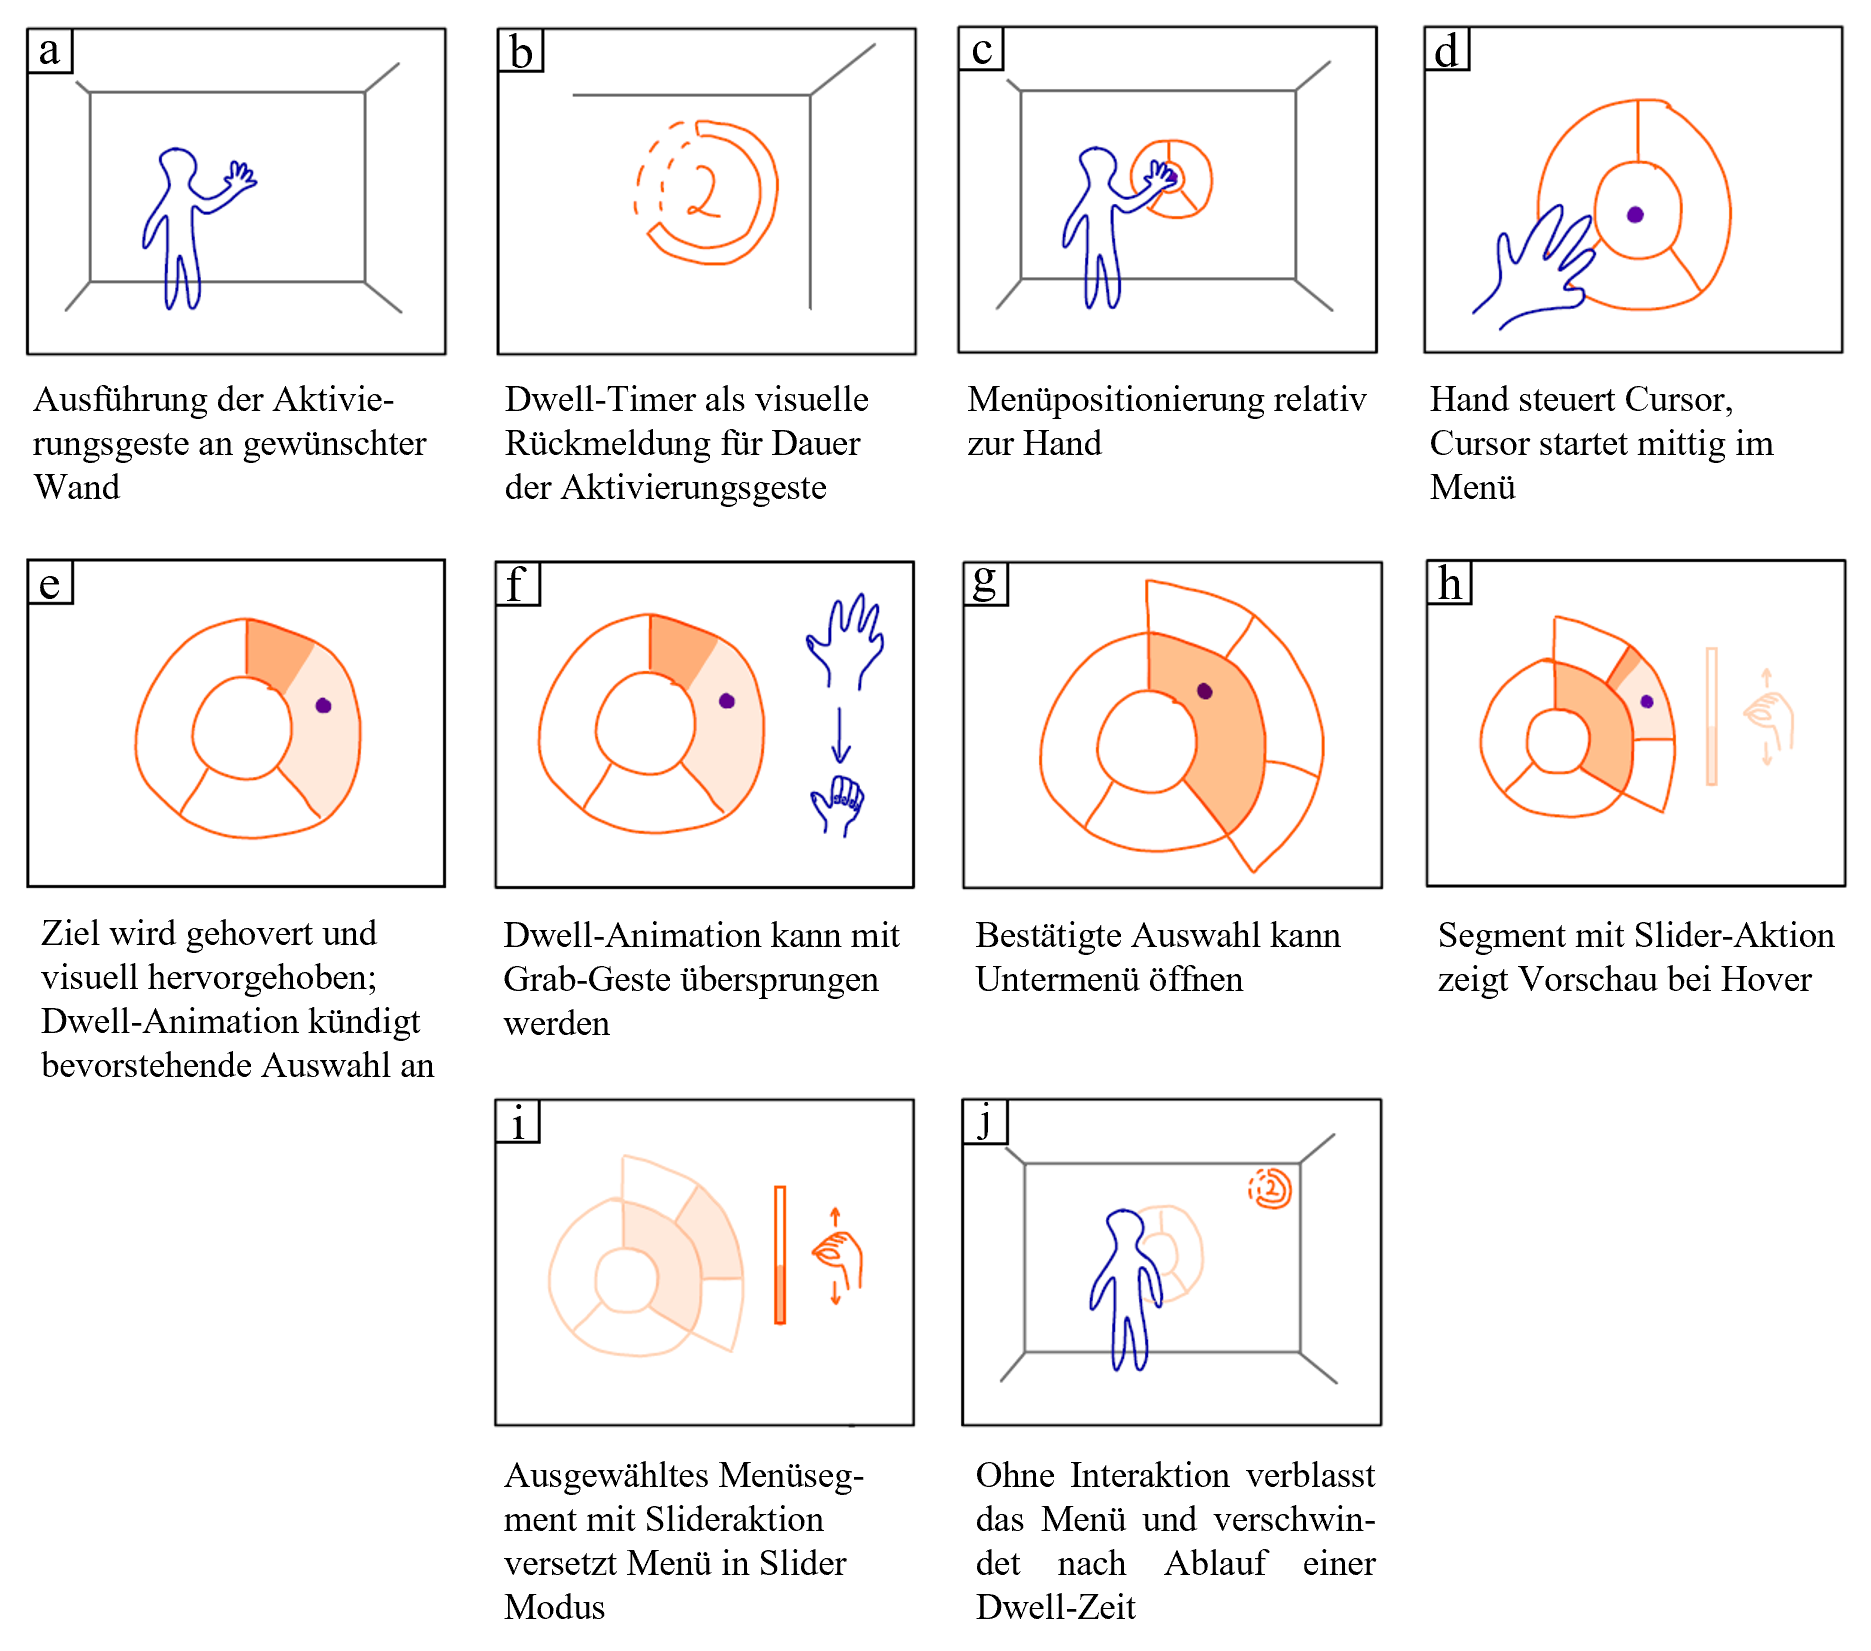
\includegraphics[width=0.98\linewidth]{content/images/storyboard_menu.png}
    \caption{Storyboard Administrative Steuerung {\color{red} Soll ich hier lieber nur 4 Pro Reihe machen, damit der Text größer ist?}}
    \label{fig:storyboard_menu}
\end{figure}


\subsubsection{Storyboard: Objektinteraktion}
Das zweite Storyboard beschreibt ein Konzept zur Objektinteraktion innerhalb der projizierten Szene.

Nach Auswahl einer Projektion positionieren sich die Nutzer:innen vor der Projektionsfläche (Abb.~\ref{fig:storyboard_paint}, a). Durch Annäherung an die Wand und das Anheben der Hand wird auch hier ein quasi-modaler Interaktionszustand aktiviert, um unbeabsichtigte Eingaben zu vermeiden und eine bewusste Interaktionsaufnahme zu ermöglichen (vgl. Abschnitt~\ref{sec:rw_midair}).

Die Handposition fungiert dabei als Cursor (Abb.~\ref{fig:storyboard_paint}, b) und überträgt ein etabliertes Interaktionsprinzip aus Desktopumgebungen in den räumlichen Kontext (vgl. \ref{sec:rw_gestures}). Dadurch bleibt die Interaktion an nachvollziehbare, körpernahe Bewegungen gekoppelt.

Gezielte Gesten ermöglichen das Setzen von Markierungen: Ein kurzer Point-and-Draw-Sweep hebt relevante Strukturen hervor (in medizinischen Szenarien beispielsweise Knochen, Muskeln oder Röntgenansichten) (Abb.~\ref{fig:storyboard_paint}, c). Dabei orientiert sich das Konzept bewusst an bekannten Handlungsmetaphern wie Zeichnen und Greifen, um eine möglichst verständliche Interaktion zu unterstützen.

Die Selektion bestehender Markierungen erfolgt über eine Grab-Geste, die das Greifen physischer Objekte imitiert. Durch Halten der Geste können Markierungen entfernt werden (Abb.~\ref{fig:storyboard_paint}, d–e).

Das Konzept adressiert damit zentrale Interaktionsaufgaben räumlicher Systeme, insbesondere Selektion und Manipulation, wie sie in Abschnitt \ref{sec:rw_spatial} eingeführt wurden, und dient als Grundlage für die weitere Ausgestaltung inhaltsbezogener Interaktionen im MIR.

\begin{figure}[H]
    \centering
    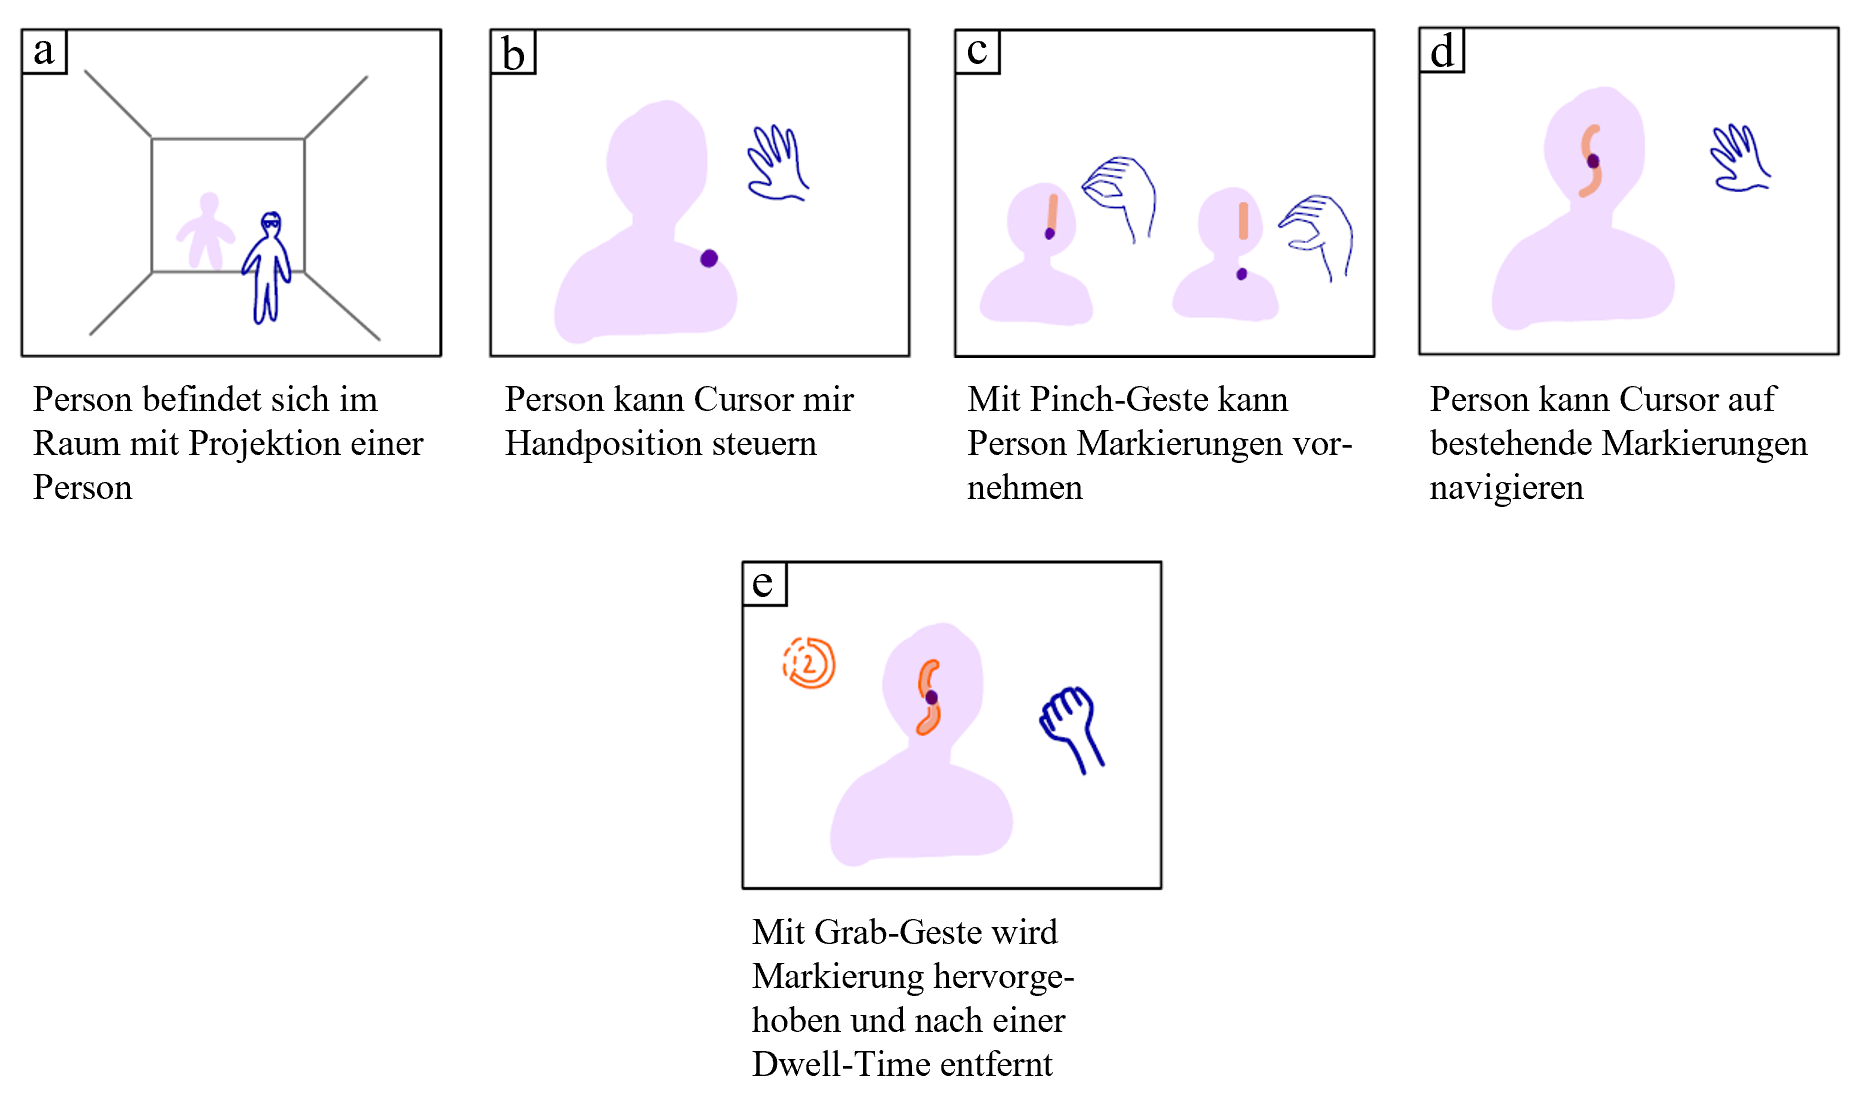
\includegraphics[width=0.98\linewidth]{content/images/storyboard_paint.png}
    \caption{Storyboard Objektinteraktion}
    \label{fig:storyboard_paint}
\end{figure}


\subsubsection{Storyboard: Navigation im Raum}
Das dritte Storyboard (Abb. \ref{fig:storyboard_navigation}) skizziert zwei Konzepte für positionsbasierte Navigation, die die körperliche Bewegung der Nutzer:innen als primären Interaktionsparameter nutzen, um eine Fortbewegung in der virtuellen Szene ohne zusätzliche Eingabegeräte zu ermöglichen.

Der erste Ansatz basiert auf einer schubbasierten Navigation (Abb. \ref{fig:storyboard_navigation}, a-c), die als steering-based Methode klassifiziert werden kann (vgl. \ref{sec:rw_navigation}). Hierbei bewegen sich Nutzer:innen in die gewünschte Richtung und initiieren die Fortbewegung durch eine aktive Schubbewegung mit den Händen. Diese explizite Kopplung von Position, Geste und virtueller Bewegung ermöglicht eine hohe Kontrolle und kann als besonders immersive Interaktionsform gelten, da Körperbewegung und virtuelle Fortbewegung eng aufeinander bezogen sind (vgl. Abschnitt~\ref{sec:rw_navigation})

% TODO FIX Satz
Der zweite Ansatz nutzt Walking-in-Place (vgl. \ref{sec:rw_navigation}), also das Gehen auf der Stelle als Auslöser virtueller Fortbewegung. Auch hier richten sich die Nutzer:innen zunächst in die Richtung aus, in die navigiert werden soll (Abb. \ref{fig:storyboard_navigation}, d-e). Die Bewegung wird durch eine Laufgeste auf der Stelle eingeleitet und aktiviert nach einer kurzen Verweildauer die Navigation im Raum (Abb. \ref{fig:storyboard_navigation}, f), welche durch die Bewegung der Szene in die entsprechende Richtung eine kontinuierliche Fortbewegung simuliert (Abb. \ref{fig:storyboard_navigation}, g). Die Bewegung endet, sobald die Nutzer:innen ihre Position verändern oder Walking-in-Place stoppen. Diese Methode ist besonders für physisch begrenzte Räume wie den MIR geeignet, da sie die kognitiven Vorteile natürlicher Fortbewegung simuliert, ohne ein großes Platzangebot vorauszusetzen.

Beide Ansätze verfolgen das Ziel, Navigation ohne zusätzliche Eingabegeräte zu ermöglichen und die körperliche Bewegung im Raum als primären Interaktionsparameter zu nutzen. Während die schubbasierte Variante eine aktive und bewusst gesteuerte Interaktion darstellt,
etzt die Walking-in-Place-Variante auf eine reduzierte zusätzliche Gestik und eine stärker bewegungsbasierte Steuerung.

Das Storyboard illustriert damit unterschiedliche Ausprägungen positionsbasierter Navigation und dient als Grundlage für die weitere Auswahl und Ausarbeitung geeigneter Interaktionskonzepte im MIR.

\begin{figure}[H]
    \centering
    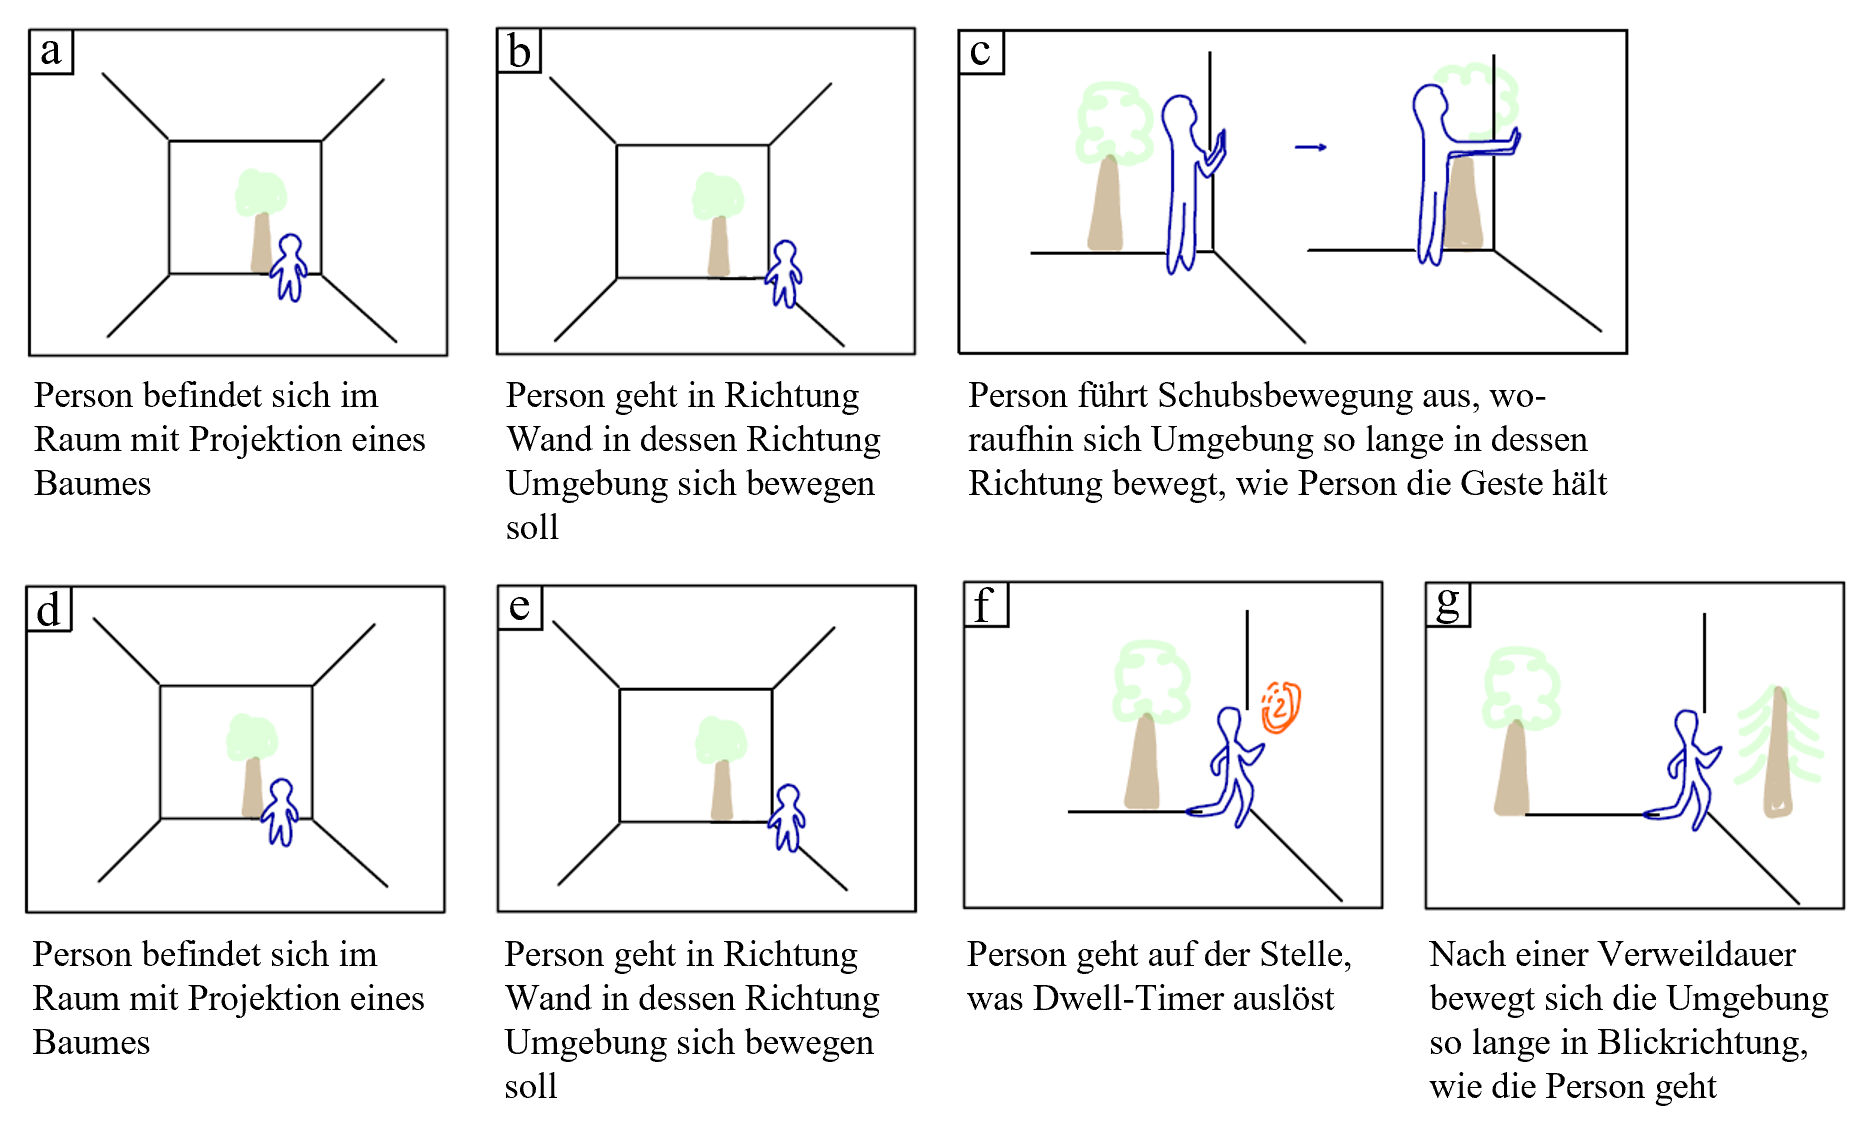
\includegraphics[width=0.98\linewidth]{content/images/storyboard_navigation.png}
    \caption{Storyboard für Navigation im Raum}
    \label{fig:storyboard_navigation}
\end{figure}


\subsection{Auswahl eines geeigneten Interaktionsparadigmas}
%Obwohl das Öffnen des Menüs eine temporäre Unterbrechung der atmosphärischen Erfahrung darstellt, ermöglicht es eine strukturierte, konsistente und lernbare Interaktion. Die Nutzer:innen können sich auf die Auswahl konzentrieren, ohne sich für jede Einstellung eine eigene Geste merken zu müssen. Die Unterbrechung ist kurz, aber notwendig, um die Komplexität der multisensorischen Steuerung zu reduzieren.


%Die Kombination aus diskreter Auswahl über das Marking Menu und kontinuierlicher Anpassung über einen Slider stellt einen sinnvollen Kompromiss dar. Während die Auswahl über das Menü strukturiert und lernbar ist, ermöglicht der Slider eine feine, kontinuierliche Anpassung – ohne dass Nutzer:innen für jede Einstellung eine eigene Geste erlernen müssen. Dies reduziert die kognitive Belastung und erhöht die Effizienz, ohne die Immersion vollständig zu unterbrechen.

Die im Rahmen der konzeptionellen Exploration entwickelten Storyboards repräsentieren drei grundlegende Interaktionsansätze im MIR: administrative Steuerung über ein Menü, objektbasierte Interaktion innerhalb der Szene sowie positionsbasierte Navigation im Raum. 

Diese drei Ansätze unterscheiden sich hinsichtlich ihrer Übertragbarkeit auf bestehende MIR-Szenarien. Die positionsbasierte Navigation setzt voraus, dass Bewegung im Raum selbst Teil der Anwendung ist, etwa im Sinne freier Fortbewegung innerhalb einer virtuellen Umgebung. Wie die Analyse der bestehenden MIR-Szenarien gezeigt hat (Abschnitt \ref{sec:analyse}), ist dies derzeit jedoch nur im Dschungel-Szenario vertreten. Für die überwiegend vorgerenderten Anwendungsszenarien ist dieser Ansatz daher nur eingeschränkt geeignet.

Auch objektbasierte Interaktionen sind nur limitiert generalisierbar. Sie setzen explizite Interaktionsobjekte oder markierbare Inhalte innerhalb der Szene voraus und erfordern damit eine entsprechende Gestaltung oder Anpassung der jeweiligen Anwendung. Da viele der bestehenden MIR-Szenarien keine solchen Interaktionspunkte vorsehen, ist dieser Ansatz nur eingeschränkt auf das Gesamtsystem übertragbar.

Im Gegensatz dazu ist eine administrative Steuerung über ein Menü unabhängig von der konkreten Szenariostruktur einsetzbar. Sie ermöglicht den Zugriff auf systemweite Funktionen, ohne dass die zugrunde liegenden Anwendungen angepasst werden müssen, und weist damit eine hohe Generalisierbarkeit auf. Beispielsweise sind allgemeine Einstellungen wie Lautstärke, Helligkeit und Vibrationsintensität in den meisten Szenarien relevant und unabhängig von deren konkreter Struktur zugänglich.
Sie ermöglichen eine controllerlose Bedienung und lassen sich direkt an natürliche Handbewegungen der Nutzer:innen koppeln. Damit unterstützen sie zentrale Anforderungen wie die Nutzung ohne zusätzliche Eingabegeräte (R2) sowie die Erhaltung der Bewegungsfreiheit im Raum (R3). Diese Einschätzung deckt sich mit den in Abschnitt \ref{sec:rw} dargestellten Potenzialen körperbasierter und Mid-Air-basierter Interaktion (vgl. Abschnitt~\ref{sec:rw_embodied} und Abschnitt~\ref{sec:rw_midair}).

Gleichzeitig stellt die Gestaltung geeigneter Interaktionsmechanismen im dreidimensionalen Raum eine Herausforderung dar.
Abschnitt~\ref{sec:rw_midair} und Abschnitt~\ref{sec:rw_menus} zeigen, dass klassische grafische Benutzungsschnittstellen nur eingeschränkt auf Mid-Air-Interaktionen übertragbar sind, da sie in der Regel für zweidimensionale Displays und präzise Eingabegeräte optimiert wurden.

Komplexe gestenbasierte Interaktionssysteme wurden im Rahmen dieser Arbeit jedoch bewusst nicht als primärer Interaktionsmechanismus gewählt. Obwohl Gesten eine natürliche Form körperbasierter Interaktion darstellen, weisen solche Systeme mehrere Herausforderungen auf. Wie in den verwandten Arbeiten dargestellt, gehen freie Gestensysteme häufig mit einer geringen Discoverability, einer erhöhten Lernanforderung sowie dem Risiko unbeabsichtigter Aktivierungen einher (vgl. Abschnitt~\ref{sec:rw_midair} und Abschnitt~\ref{sec:rw_gestures}). Darüber hinaus können Gestenerkennungssysteme in offenen Interaktionsräumen zu Fehlinterpretationen führen, wenn alltägliche Bewegungen fälschlicherweise als Interaktion interpretiert werden.

Um diese Herausforderungen zu adressieren, wurde ein menübasiertes Interaktionskonzept gewählt, das verfügbare Funktionen explizit sichtbar macht und gleichzeitig eine gestenbasierte Steuerung ermöglicht. Wie in Abschnitt~\ref{sec:rw_menus} gezeigt, eignen sich Marking-Menus besonders für solche Kontexte, da sie kurze Zielwege, eine hohe Erlernbarkeit und die Unterstützung motorischen Lernens kombinieren.
Vor diesem Hintergrund wurden Marking-Menus als zentrales Interaktionsparadigma für den MIR ausgewählt.


\subsection{Konzeption des Interaktionssystems} % Hauptkapitel + hier nochmal Requirements erwähnen?
\label{sec:synthese_konzeption_des_interaktionssystems}


% ZUSAMMENGEFASST MIT QUELLEN:

% Bei der Auswahl eines Schiebereglers tritt das Menü visuell zurück, um den Fokus zu lenken. Eine Pinch-Geste, die an die Nutzung physischer Regler erinnert, wird durch ein Icon eingeführt, um von bekannten Metaphern zu profitieren \parencite{LaViola20043DUserInterfaces, jacob2008realitybasedinteraction}.


Auf Basis der getroffenen Auswahl wird das Konzept einer menübasierten, gestenbasierten Interaktion im Folgenden weiter konkretisiert. Während das Storyboard bereits die grundlegende Interaktionsidee und den Nutzungskontext skizziert, liegt der Fokus dieses Kapitels auf der detaillierten Ausgestaltung des Interaktionsmechanismus.

Dabei werden zentrale Designentscheidungen hinsichtlich Struktur, Interaktionsablauf und visueller Gestaltung des radialen Menüs hergeleitet. \\

Das entwickelte Interaktionskonzept kombiniert kamerabasiertes Handtracking mit einem radialen Menü, das als zentrale Interaktionsschnittstelle zwischen Nutzer:innen und Zielanwendung fungiert. Die Position der Hand im Raum wird dabei als Cursor interpretiert, über den Nutzer:innen mit dem Menü interagieren können. Das Menü wird als Overlay über der jeweiligen Zielanwendung eingeblendet und ermöglicht den Zugriff auf systemweite Steuerungsfunktionen, ohne dass die bestehende Anwendung angepasst werden muss.

Durch diese Entkopplung von Interaktion und Anwendung wird eine flexible und szenariounabhängige Nutzung des Systems ermöglicht.


\subsubsection{Handtracking und Cursor}
\label{sec:synthese_handtracking}

Die Position der Hand im Raum wird als primärer Interaktionspunkt genutzt und dient als Cursor innerhalb des Overlays. Die Interpretation der Handposition orientiert sich bewusst an bekannten Interaktionsmustern aus etablierten Benutzungsoberflächen und überträgt diese in den räumlichen Kontext. Die Nutzung dieses Prinzips soll dazu beitragen, dass Nutzer:innen das System und die Steuerungsmöglichkeiten ohne vorherige Anleitung anwenden können (vgl. Abschnitt~\ref{sec:rw_gestures} zu Evolutionary Gestures).

Im Gegensatz zu klassischen Eingabegeräten wie Maus oder Controller entsteht dadurch eine direkte räumliche Beziehung zwischen Nutzerbewegung und Systemreaktion. Gleichzeitig können Nutzer:innen ihre Hände frei im Raum bewegen, wodurch die Interaktion mit der natürlichen Bewegungsfreiheit im MIR vereinbar bleibt (R3). \\

{\color{red} Ist es störend, dass ich hier von der Menüpositionierung spreche? Aber eigentlich ist es ja wichtig um zu verstehen, wieso die Cursorposition so gewählt wird + als Kontext für den Interaktionsraum}
Das Menü und der Cursor werden standardmäßig nicht angezeigt, sondern muss durch Nutzer:innen mit einer Aktivierungsgeste (vgl. Abbildung \ref{fig:openpalm_gesture_image_no_marking}) erst aktiviert werden. Dies verhindert die versehentliche Auslösung der Menüinteraktion (vgl. Abschnitt~\ref{sec:rw_midair}), sodass die Immersion der Zielanwendung nicht unbeabsichtigt unterbrochen wird. Nach erfolgreicher Aktivierung wird das Menü an einer festen Position im Raum eingeblendet, standardmäßig in der Mitte des aktiven Bildschirms. Der Cursor wird jedoch initial im Zentrum positioniert, sodass die Interaktion relativ zu diesem Ausgangspunkt erfolgt. Dadurch entsteht ein lokaler Interaktionsraum um die Aktivierungsposition herum (vgl. Abb.~\ref{fig:Interaktionsraum}), der unabhängig von der Körpergröße oder Haltung der Nutzer:innen genutzt werden kann. Diese Gestaltung ermöglicht eine konsistente und ergonomische Interaktion, da Nutzer:innen das Menü aus unterschiedlichen Positionen im Raum heraus aktivieren können, ohne dass die relative Erreichbarkeit der Menüelemente beeinflusst wird. Zugleich adressiert sie die in Abschnitt~\ref{sec:rw_midair}  beschriebenen Ermüdungsprobleme länger gehaltener Mid-Air-Interaktion, da Nutzer:innen selbst bestimmen können, in welcher Haltung die Interaktion am komfortabelsten für sie ist.

\begin{figure}[H]
    \centering
    \begin{subfigure}{0.27\textwidth}
        \centering
        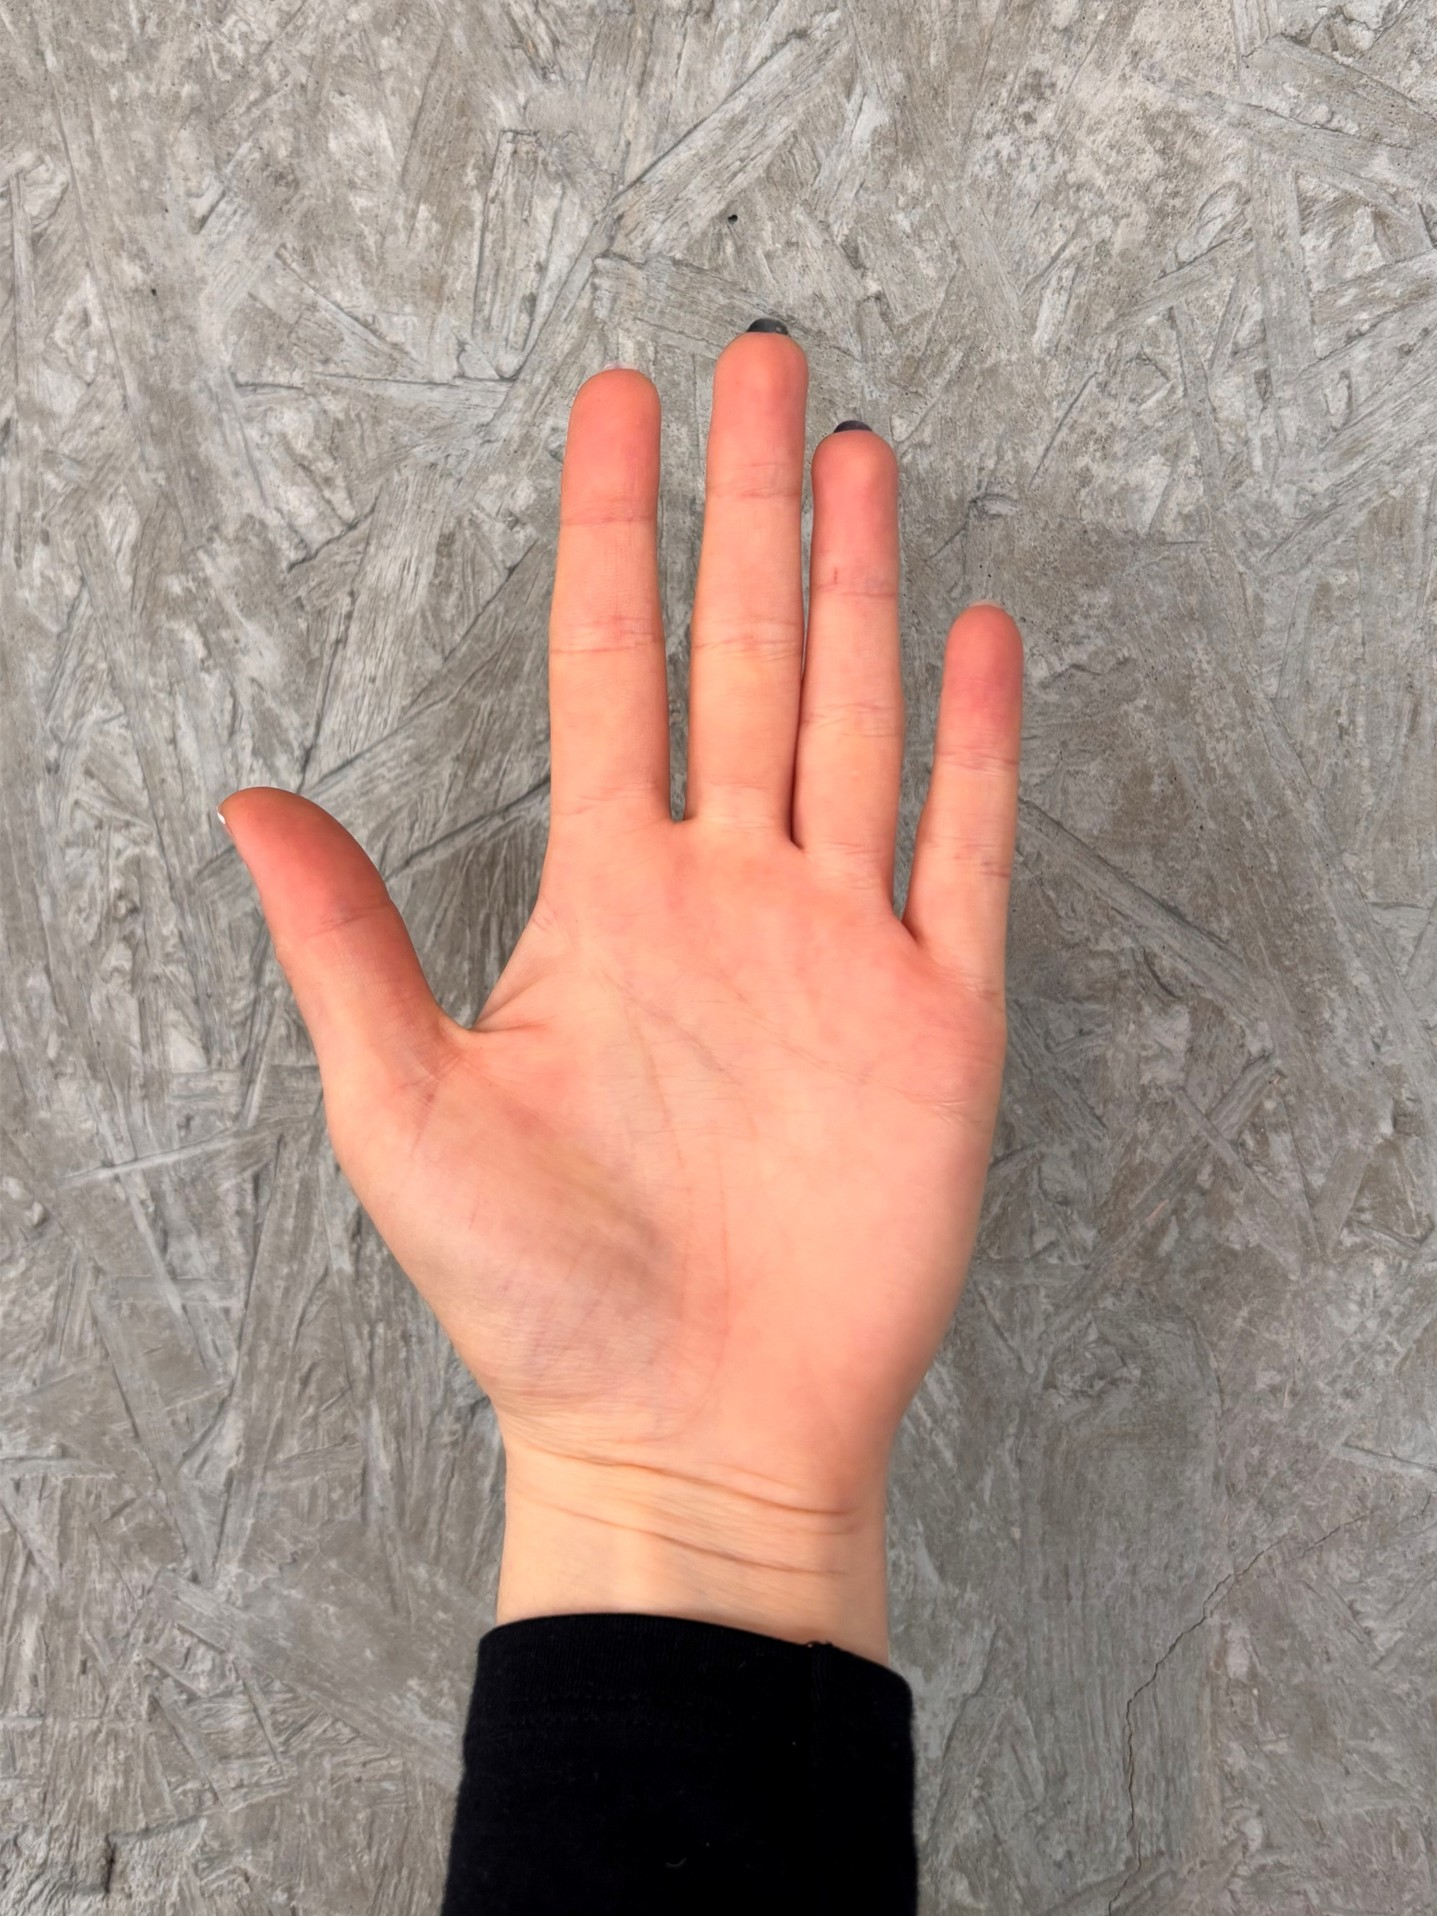
\includegraphics[
            width=\linewidth
        ]{content/images/open_palm.jpg}
        \caption{Aktivierungsgeste}
        \label{fig:openpalm_gesture_image_no_marking}
    \end{subfigure}
    \hspace{0.5cm}
    \begin{subfigure}{0.65\textwidth}
        \centering
        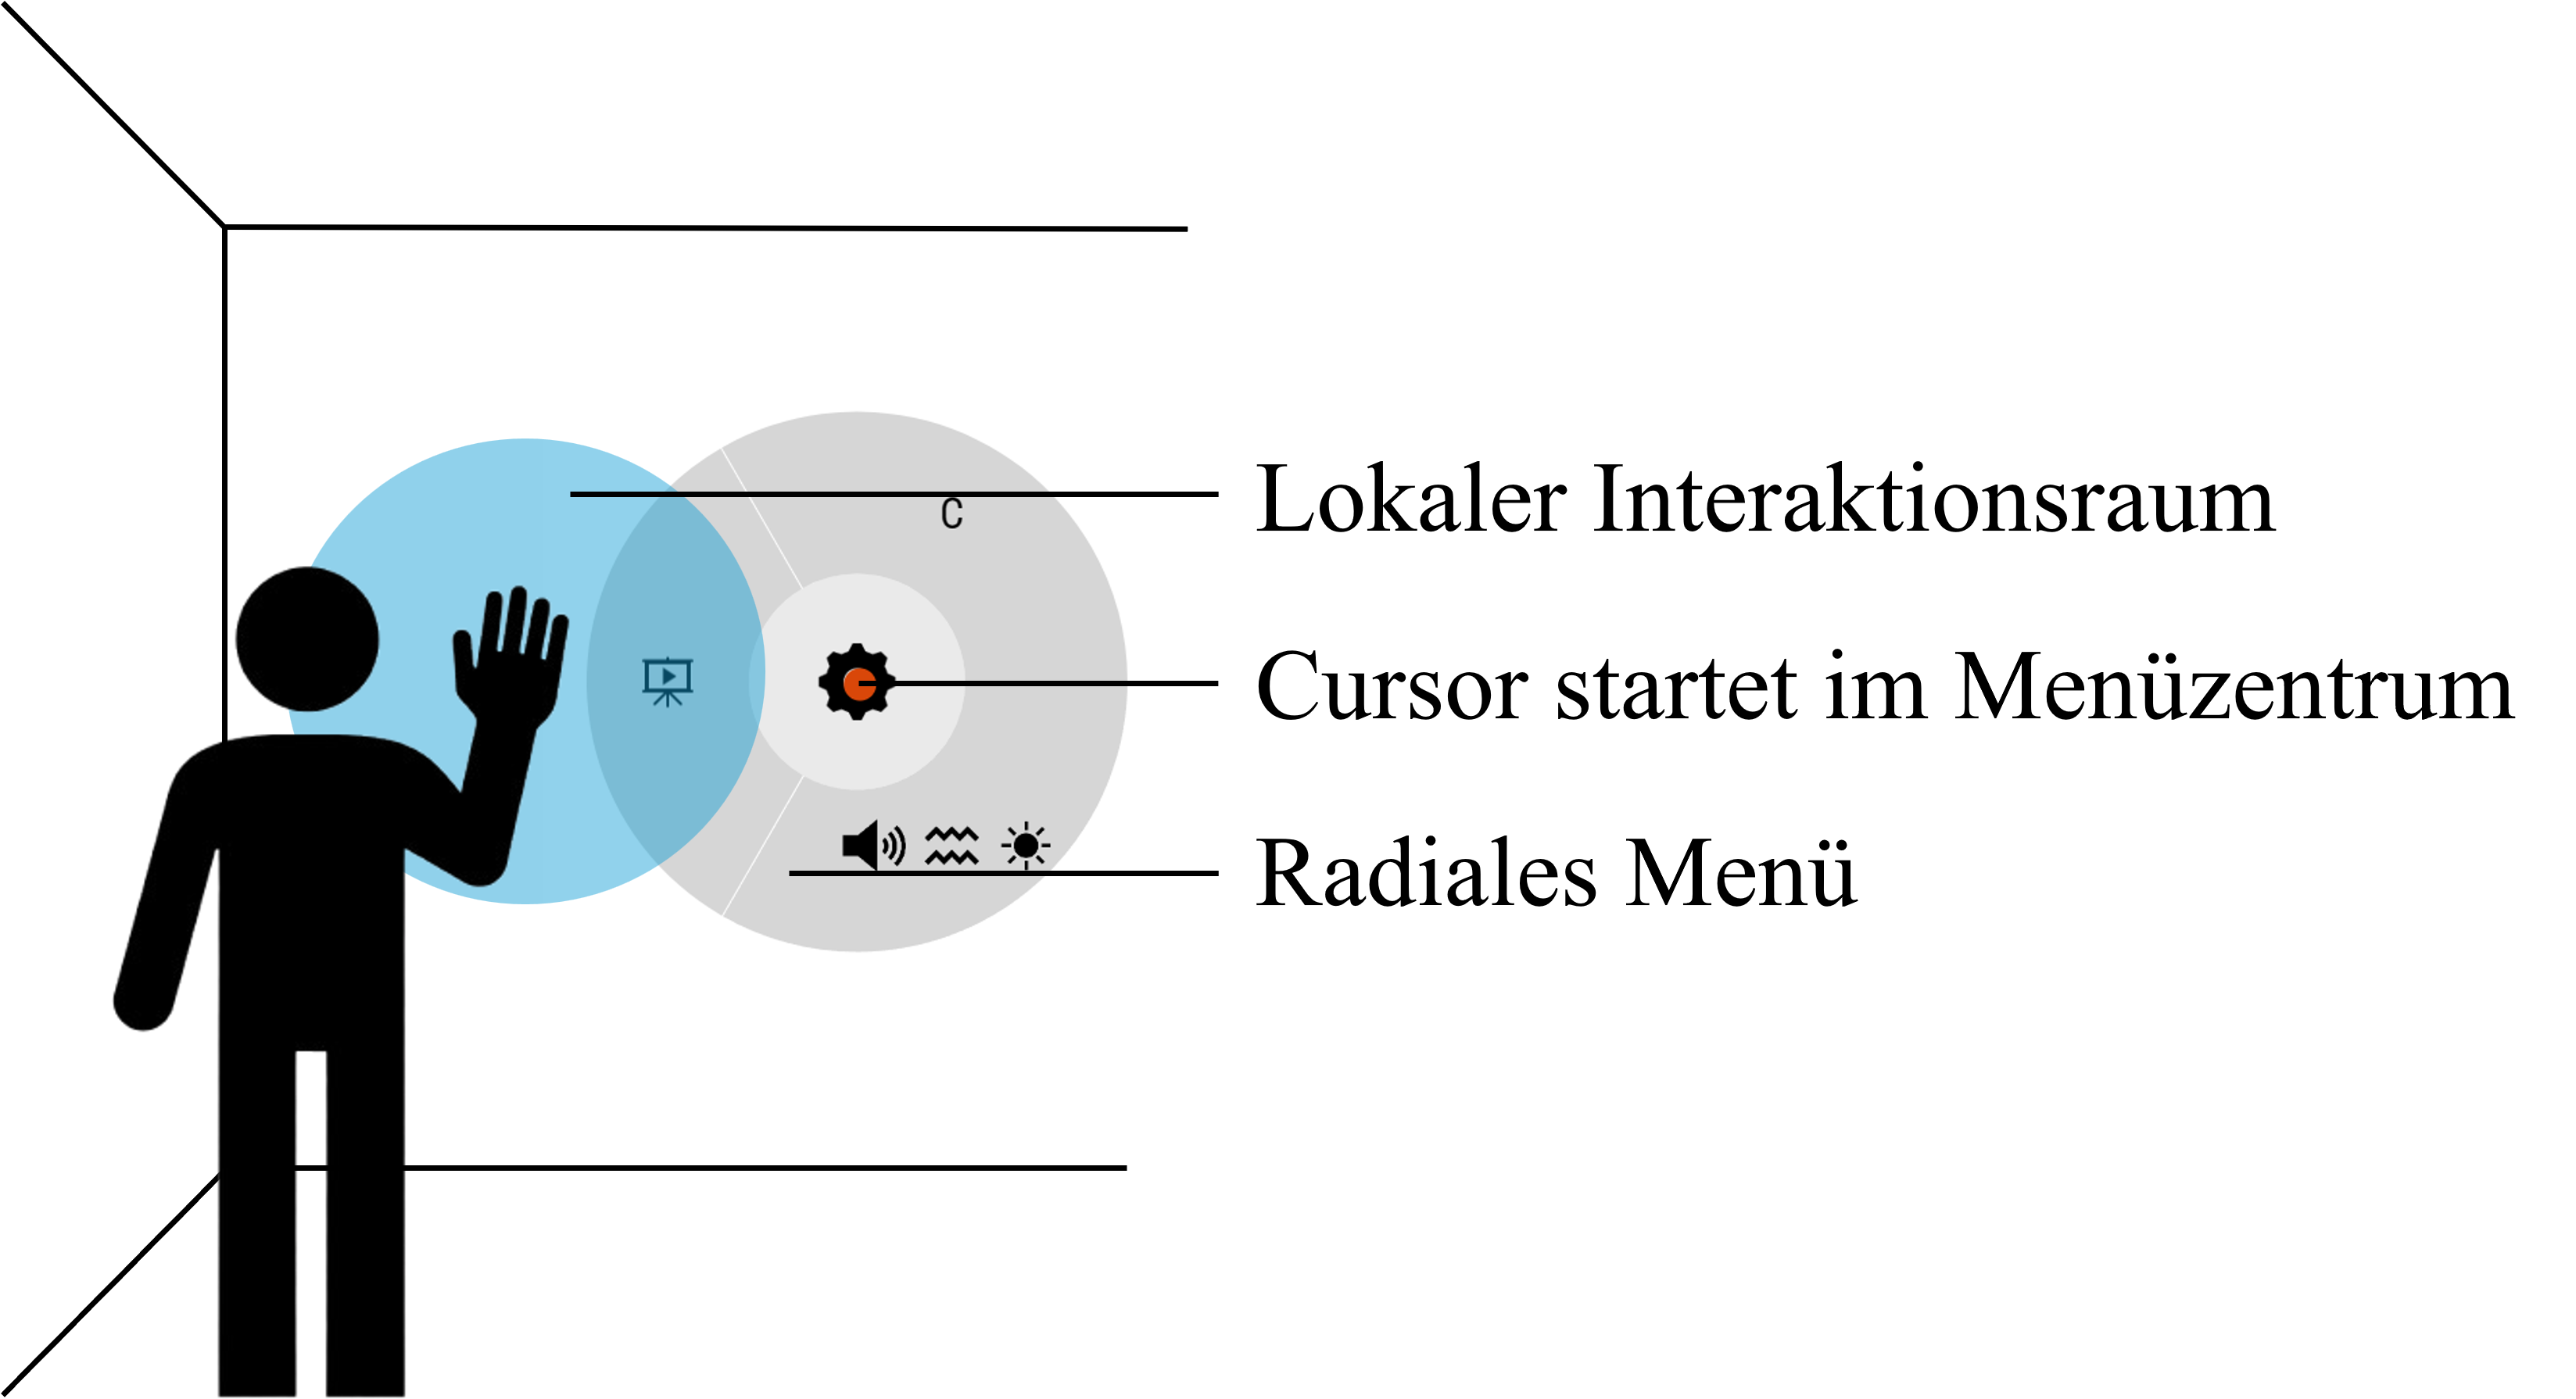
\includegraphics[
            width=\linewidth
        ]{content/images/Interaktionsraum.png}
        \caption{Schematische Darstellung des Interaktionsraums}
        \label{fig:interaktionsraum}
    \end{subfigure}
    \caption{Darstellung der Aktivierungsgeste und des lokalen Interaktionsraums}
    \label{fig:interaction_start}
\end{figure}

Zur weiteren Vereinfachung der Interaktion wird nicht zwischen linker und rechter Hand unterschieden. Dadurch wird die Komplexität reduziert und die Bedienbarkeit erhöht, da Nutzer:innen beliebig die Interaktionshand wechseln können.

Die Hand fungiert somit als zentraler Interaktionsanker, über den Auswahl- und Steuerungsaktionen ausgeführt werden können. Dadurch kann auf zusätzliche Eingabegeräte verzichtet werden, während gleichzeitig eine natürliche und intuitive Interaktion ermöglicht wird.


\subsubsection{Radiales Menü}
\label{sec:synthese_radiales_menü}
Als zentrale Interaktionsschnittstelle wurde ein Marking-Menu als gestanbasierte Variante eines radialen Menüs gewählt. Diese Entscheidung knüpft an die in Abschnitt~\ref{sec:rw_menus} dargestellten Vorteile dieser Menüform für Mid-Air-Interaktion an, insbesondere an kurze Zielwege, gleichmäßige Erreichbarkeit und die Unterstützung motorischen Lernens.

{\color{red} TODO: Hier könnte auch abschnitt über Menüpositionierung rein - eher hier oder in Handtracking (?) - meine tendenz handtracking}

Vor dem Hintergrund der in Abschnitt~\ref{sec:rw_menus} diskutierten Zusammenhänge zwischen Menütiefe, Segmentbreite und Präzision wird eine moderate Anzahl an Einträgen pro Ebene angestrebt, jedoch nicht erzwungen. Eine hohe Anzahl von Segmenten führt dazu, dass die einzelnen Einträge zunehmend kleiner werden. Dadurch verringert sich nicht nur die Interaktionsfläche für den Cursor, sondern auch der verfügbare Platz für Beschriftungen der Menüsegmente. Aus diesem Grund wurde entschieden, Icons anstelle textueller Labels zu verwenden.

Da im MIR nicht die möglichst schnelle Ausführung von Aufgaben im Vordergrund steht, sondern eine intuitive, verständliche und in den Raum eingebettete Interaktion, und die konkrete Menüstruktur maßgeblich durch die jeweilige Zielanwendung bestimmt wird, ist eine starre Begrenzung der Segmentanzahl jedoch nicht in allen Fällen zielführend. Stattdessen erscheint es sinnvoll, bei der Gestaltung auf potenzielle Usability-Probleme hinzuweisen, die sich insbesondere aus großer Menütiefe oder vielen Einträgen ergeben können.


\subsubsection{Auswahlmechanismen}
Für die Auswahl von Menüeinträgen wurden zwei unterschiedliche Interaktionsmechanismen vorgesehen: eine aktive Greifgeste sowie eine zeitbasierte Auswahl (Dwell Selection). Diese Kombination greift die in Abschnitt~\ref{sec:rw_gestures} dargestellten Vor- und Nachteile impliziter und expliziter Selektionsmechanismen auf.

Die Dwell-basierte Auswahl ermöglicht einen niedrigschwelligen Zugriff auf Menüfunktionen, da sie keine zusätzliche Bestätigungsgeste voraussetzt. Damit eignet sie sich insbesondere für Erstnutzende oder für Situationen, in denen möglichst wenig gestische Komplexität erforderlich ist. Gleichzeitig ist, wie in Abschnitt~\ref{sec:rw_gestures} diskutiert, bekannt, dass Dwell-basierte Verfahren leicht verständlich sein können, jedoch mit längeren Interaktionszeiten einhergehen können.

Zusätzlich wurde eine Greifgeste als explizite Auswahlmethode vorgesehen (Abb. \ref{fig:grab_gesture}). Dabei orientiert sich das Konzept bewusst an einer vertrauten Handlungsmetapher des Greifens und somit physichen Auswählens, um die Erlernbarkeit zu unterstützen. Um die Discoverability der expliziten Geste zu fördern, wird sie durch einen visuellen Hinweis eingeführt (Abb. \ref{fig:grab_hint}). Dies adressiert die in Abschnitt~\ref{sec:rw_gestures} diskutierte Bedeutung von Guessability und Discoverability in gestenbasierten Systemen.

\begin{figure}[H]
    \centering
    \begin{subfigure}[t]{0.27\textwidth}
        \centering
        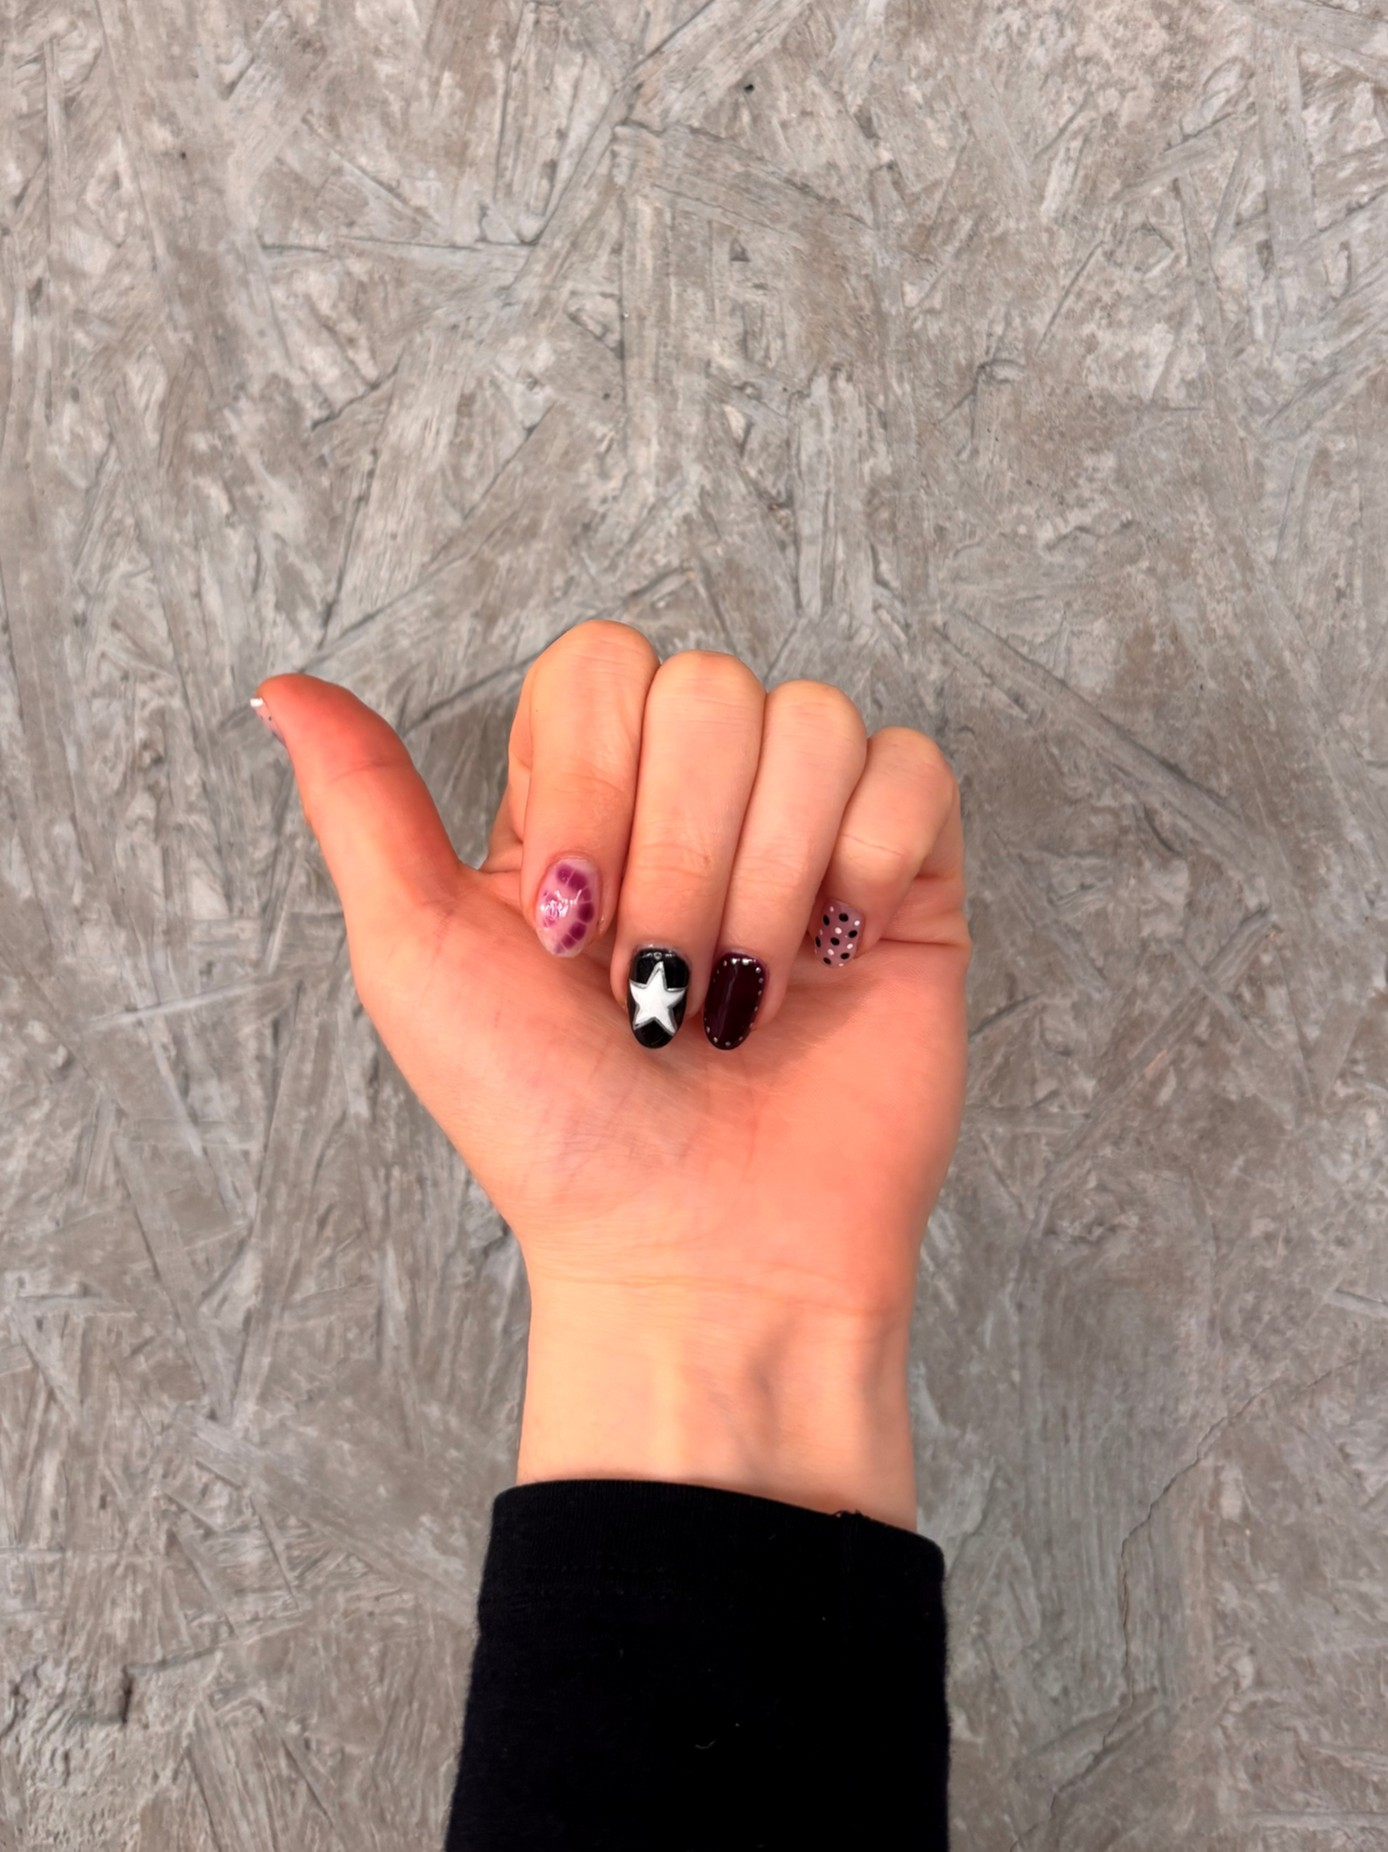
\includegraphics[
            width=\linewidth
        ]{content/images/grab_gesture.jpg}
        \caption{Grab-Geste}
        \label{fig:grab_gesture}
    \end{subfigure}
    \hspace{0.5cm}
    \begin{subfigure}[t]{0.6\textwidth}
        \centering
        
\includegraphics[
            width=\linewidth
        ]{content/images/grab_hint.png}
        \caption{Hinweisanimation, die Nutzer:innen zeigt, wie Dwell-Zeit übersprungen werden kann.}
        \label{fig:grab_hint}
    \end{subfigure}
    \caption{Darstellung der Grab-Interaktion.}
    \label{fig:grab}
\end{figure}

Durch die Kombination beider Mechanismen kann das System sowohl Einsteiger als auch erfahrene Nutzer:innen unterstützen.


\subsubsection{Visuelle Gestaltung und Zustandsrückmeldungen}

Da Mid-Air-Interaktion im Unterschied zu physischen Eingabegeräten keine direkte haptische Rückmeldung bietet, kommt der visuellen Kommunikation von Interaktionszuständen eine zentrale Rolle zu. Das Interaktionssystem sieht daher vor, relevante Zustände wie Fokussierung, Auswahl und laufende Aktivierung sichtbar zu machen. Dadurch soll jederzeit nachvollziehbar bleiben, welche Funktion aktuell adressiert wird und in welchem Zustand sich die Interaktion befindet.

Diese Form der Rückmeldung ist insbesondere vor dem Hintergrund der in Abschnitt~\ref{sec:rw_midair} beschriebenen Herausforderungen hinsichtlich Präzision, Kontrolle und Fehlinterpretation relevant. Visuelle Hinweise dienen hier nicht nur der Bestätigung erfolgreicher Eingaben, sondern auch der Reduktion von Unsicherheit während der Interaktion.

Es es sinnvoll mehrere visuelle Zustände zu planen, um den aktuellen Interaktionsstatus nachvollziehbar darzustellen. Befindet sich der Cursor über einem Menüsegment, wird dieses visuell hervorgehoben (Hover-Zustand, vgl. Abb. \ref{fig:zustandsvisualisierungen_synthese}, c). Diese Hervorhebung dient als unmittelbare Rückmeldung darüber, welches Menüelement aktuell fokussiert ist.

Wird ein Menüeintrag aktiv ausgewählt, durch eine Greifgeste oder durch das Auslösen eines Dwell-Timers, wechselt das entsprechende Segment in einen ausgewählten Zustand (Abb. \ref{fig:zustandsvisualisierungen_synthese}, b), der durch eine deutlichere Farbänderung dargestellt wird.

Während der Dwell-basierten Auswahl wird zusätzlich eine visuelle Fortschrittsanzeige eingeblendet.
Diese zeigt den zeitlichen Fortschritt der Aktivierung und ermöglicht es Nutzer:innen, den aktuellen Interaktionsstatus besser einzuschätzen (Abb. \ref{fig:zustandsvisualisierungen_synthese}, d).

{\color{red} TODO: ggf hier alte Visualisierung nehmen, wo ich noch Rahmen + pink hatte, damit implizit klar wird, dass es iterativer Stylingprozess war?}
\begin{figure}[H]
    \centering
    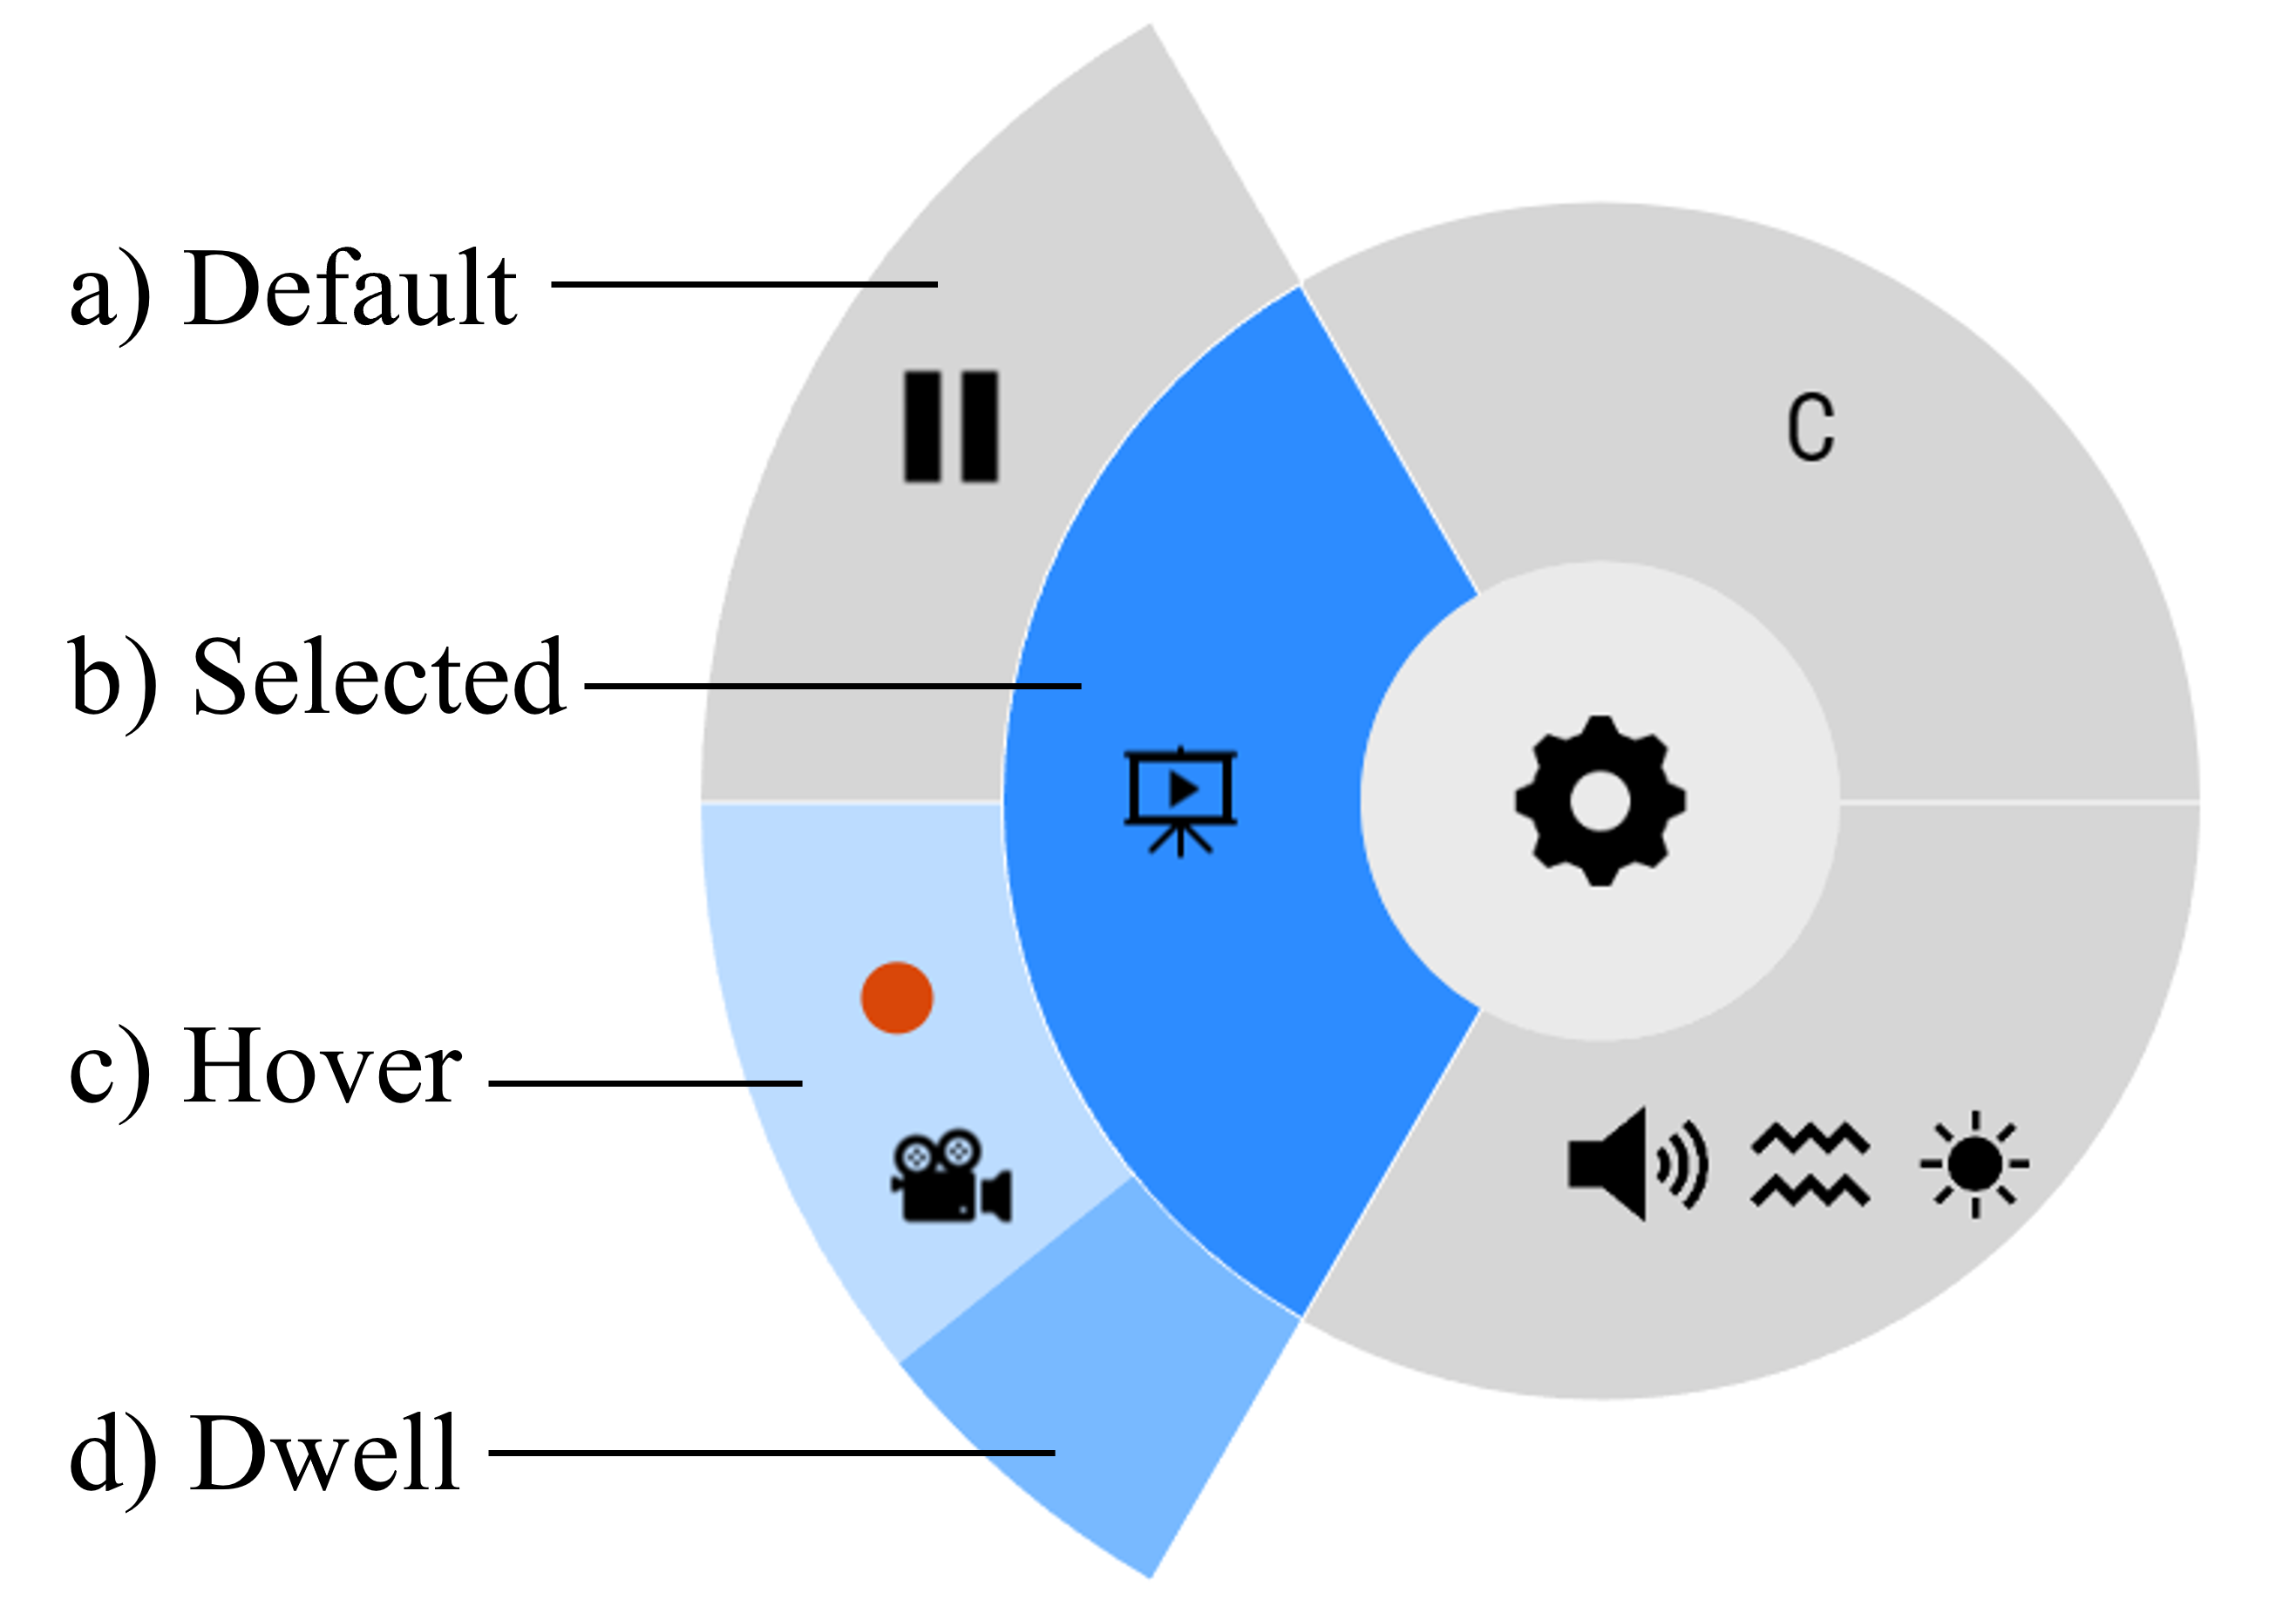
\includegraphics[width=0.5\linewidth]{content/diagrams/zustandsvisualisierungen.png}
    \caption{Verschiedene Visualisierungen des Zustands}
    \label{fig:zustandsvisualisierungen_synthese}
\end{figure}

Die konkrete visuelle Ausgestaltung wurde im Entwicklungsverlauf iterativ verfeinert.


\subsubsection{Submenus}
Um eine größere Anzahl von Funktionen innerhalb des Interaktionssystems zugänglich zu machen, wurde das radiale Menü um Submenüs erweitert. Einzelne Segmente des Hauptmenüs können weitere Menüebenen enthalten, die bei Auswahl eines Elements geöffnet werden.
Diese hierarchische Struktur ermöglicht es, thematisch zusammengehörige Funktionen zu gruppieren und gleichzeitig die visuelle Komplexität des Hauptmenüs zu reduzieren.
Menüeinträge erfüllen dabei zwei unterschiedliche Rollen: Sie können entweder als Kategorie fungieren (Abb. \ref{fig:menu_with_submenu_syn}) und ein weiteres Untermenü öffnen oder direkt eine Interaktion auslösen. Solche Interaktionen können beispielsweise diskrete Aktionen (zum Beispiel Button-Funktionen, vgl. Abb. \ref{fig:menu_with_button_syn}) oder kontinuierliche Parametersteuerungen wie Slider umfassen (Abb. \ref{fig:menu_with_slider_presentation_syn}).
Durch diese mehrstufige Organisation bleibt die Anzahl der gleichzeitig sichtbaren Menüelemente begrenzt, wodurch die Orientierung im Menü erleichtert wird und die Interaktion auch im Mid-Air-Kontext übersichtlich bleibt. Gleichzeitig erlaubt die hierarchische Struktur eine flexible Erweiterung des Systems um zusätzliche Funktionen.

\begin{figure}[H]
    \centering
    \begin{subfigure}[t]{0.3\textwidth}
        \centering
        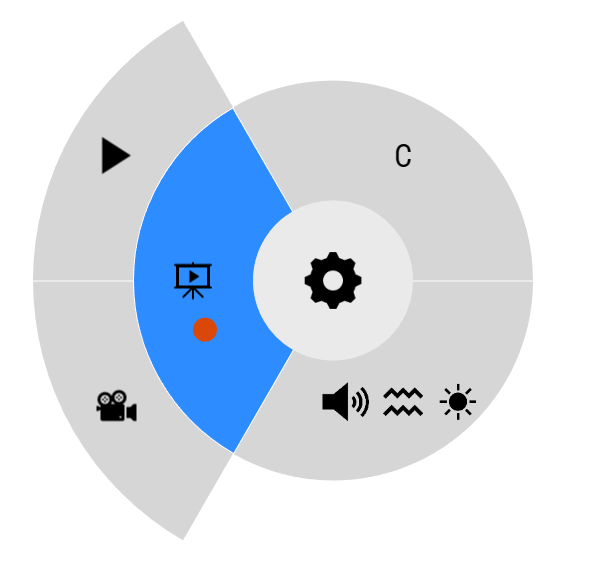
\includegraphics[width=\linewidth]{content/images/menu_with_submenu.png}
        \caption{Cursor befindet sich auf Menüelement, das ein Submenü öffnet.}
        \label{fig:menu_with_submenu_syn}
    \end{subfigure}
    \hfill
    \begin{subfigure}[t]{0.35\textwidth}
        \centering
        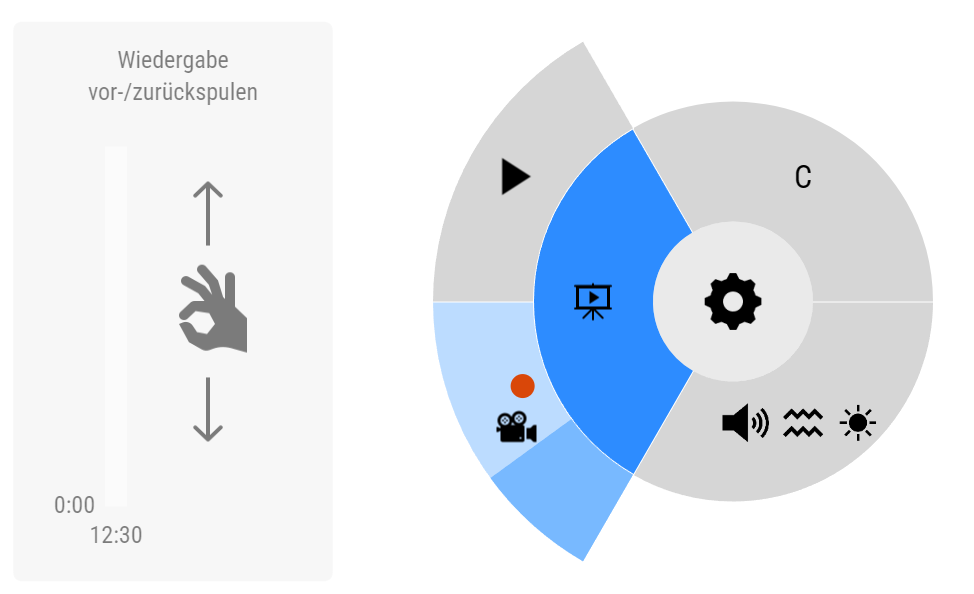
\includegraphics[width=\linewidth]{content/images/menu_with_slider_presentation.png}
        \caption{Cursor befindet sich auf Menüelement, das Slider öffnet.}
        \label{fig:menu_with_slider_presentation_syn}
    \end{subfigure}
    \hfill
    \begin{subfigure}[t]{0.3\textwidth}
        \centering
        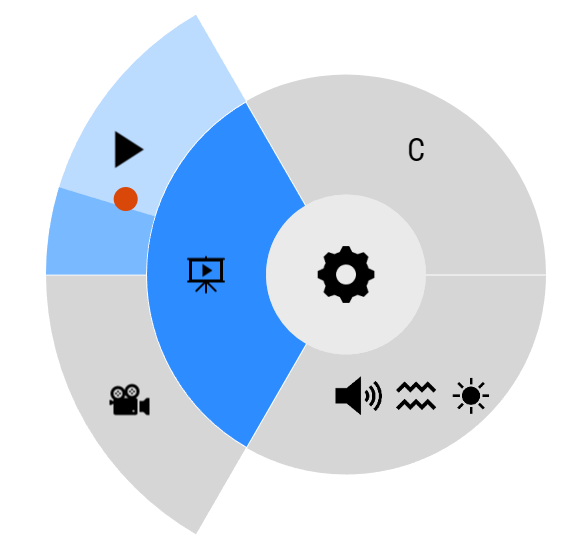
\includegraphics[width=\linewidth]{content/images/menu_with_button.png}
        \caption{Cursor befindet sich auf Menüelement, das als Button fungiert}
        \label{fig:menu_with_button_syn}
    \end{subfigure}
    \caption{Verschiedene Möglichkeit der Menüelemente}
    \label{fig:gesture_images_syn}
\end{figure}

Zum Aktivieren eines Untermenüs selektieren die Nutzer:innen einen Menüeintrag, der in der Menüstruktur über Kindelemente verfügt. Solange sich der Cursor innerhalb dieses Eintrags (Abb. \ref{fig:menu_cursor1}) oder des geöffneten Untermenüs (Abb. \ref{fig:menu_cursor2}) befindet, bleibt das Untermenü sichtbar und kann weiter genutzt werden.
Verlässt der Cursor sowohl den Menüeintrag als auch das zugehörige Untermenü (Abb. \ref{fig:menu_cursor3}), wird das Untermenü automatisch geschlossen. Durch diese kontextabhängige Sichtbarkeit bleibt die visuelle Komplexität des Menüs gering, während gleichzeitig eine größere Anzahl von Funktionen selektiv zugänglich gemacht werden kann.

\begin{figure}[H]
    \centering
    \begin{subfigure}[t]{0.32\textwidth}
        \centering
        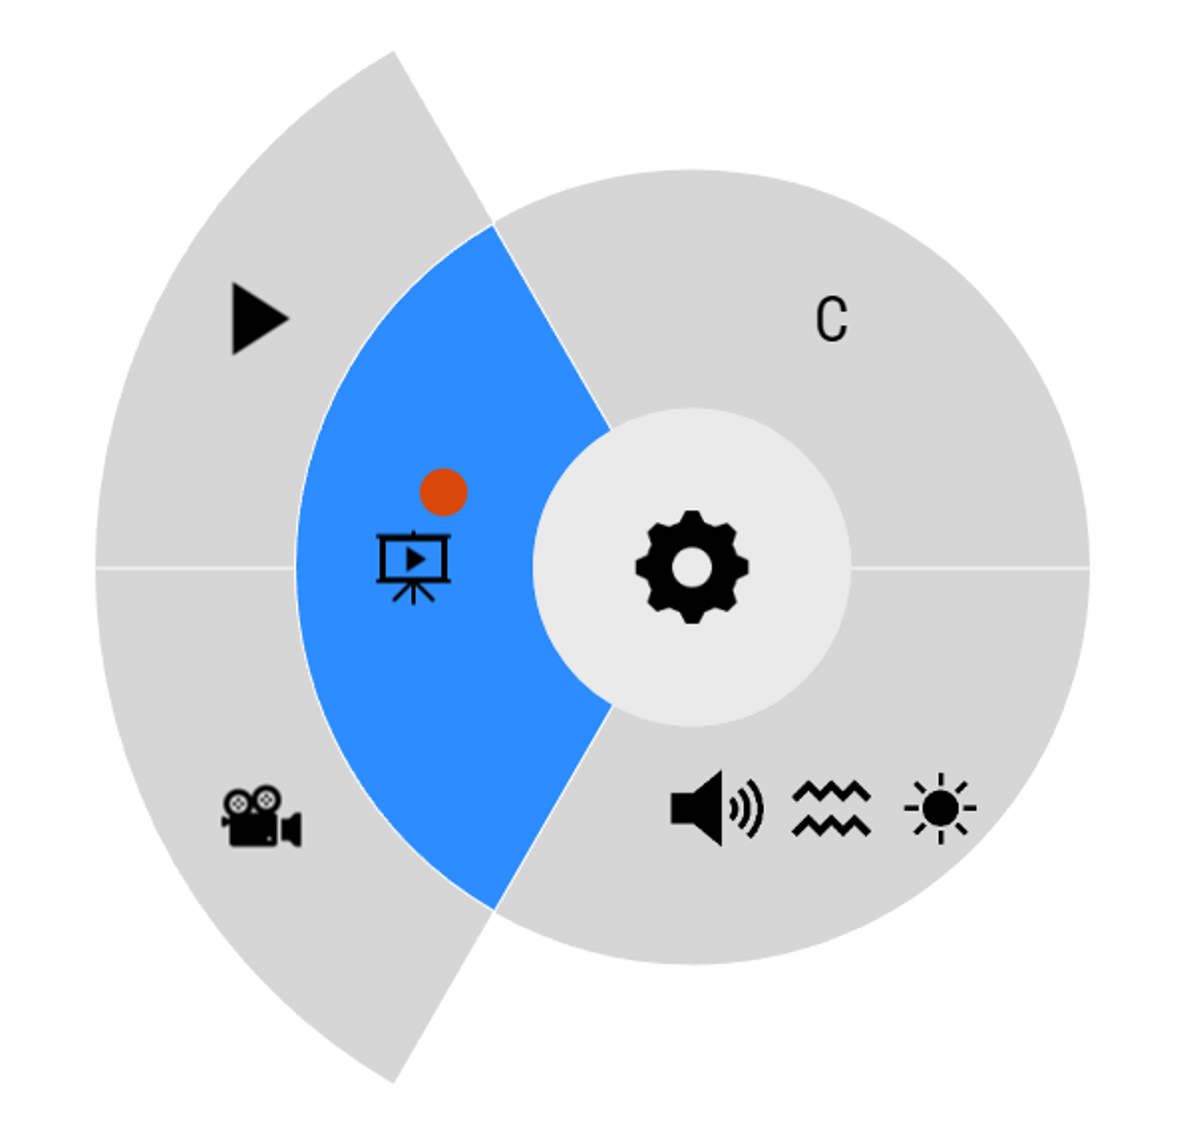
\includegraphics[width=\linewidth]{content/images/menu_cursor1.png}
        \caption{Cursor in Hauptmenüelement, nachdem Submenü geöffnet wurde.}
        \label{fig:menu_cursor1}
    \end{subfigure}
    \hfill
    \begin{subfigure}[t]{0.32\textwidth}
        \centering
        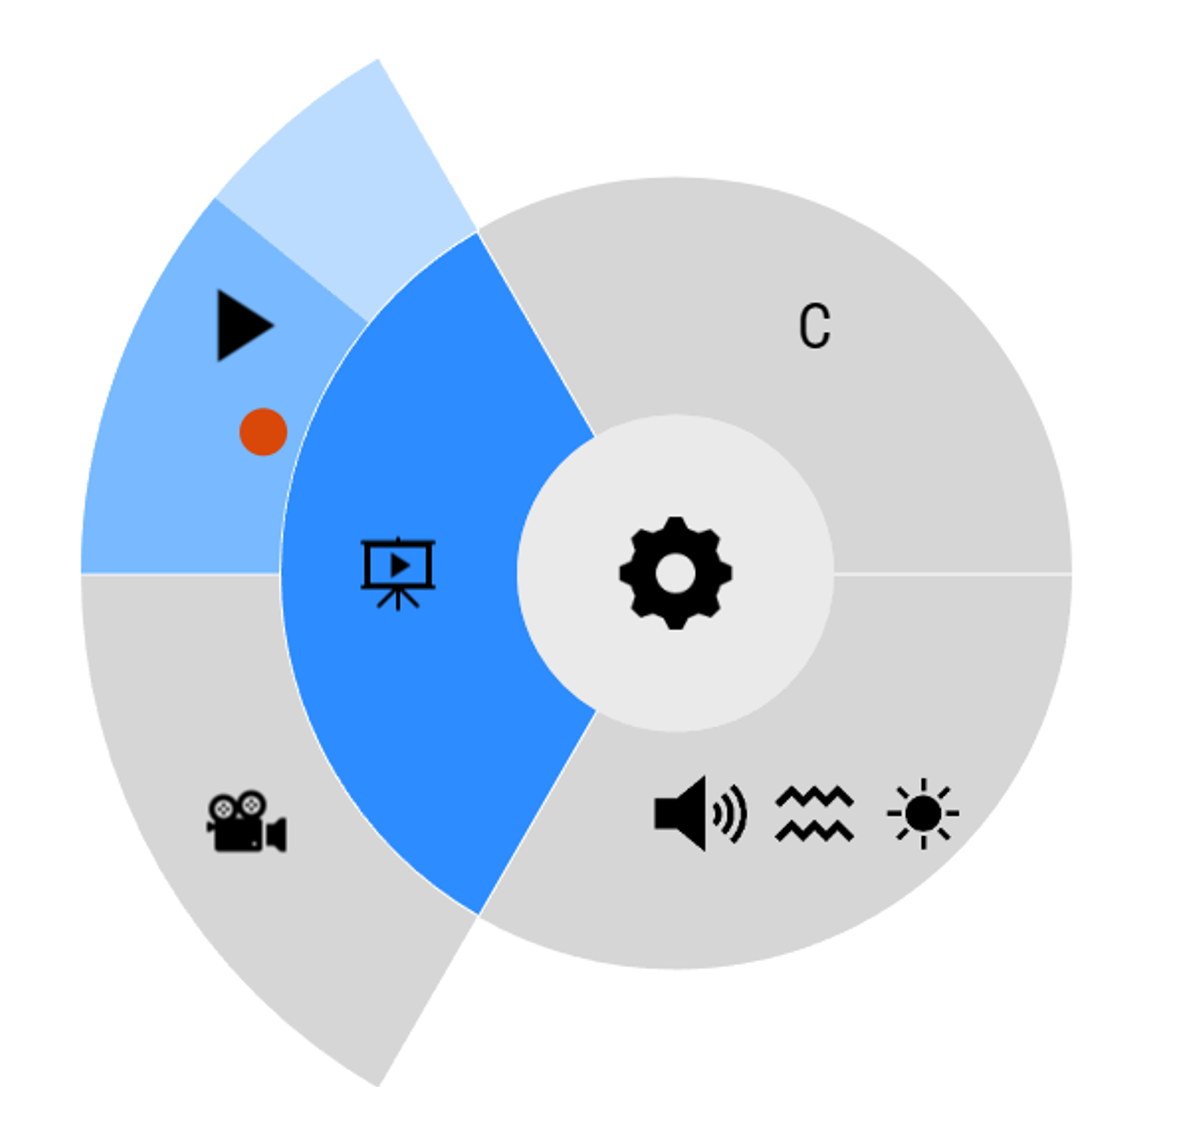
\includegraphics[width=\linewidth]{content/images/menu_cursor2.png}
        \caption{Cursor in Submenü.}
        \label{fig:menu_cursor2}
    \end{subfigure}
    \hfill
    \begin{subfigure}[t]{0.32\textwidth}
        \centering
        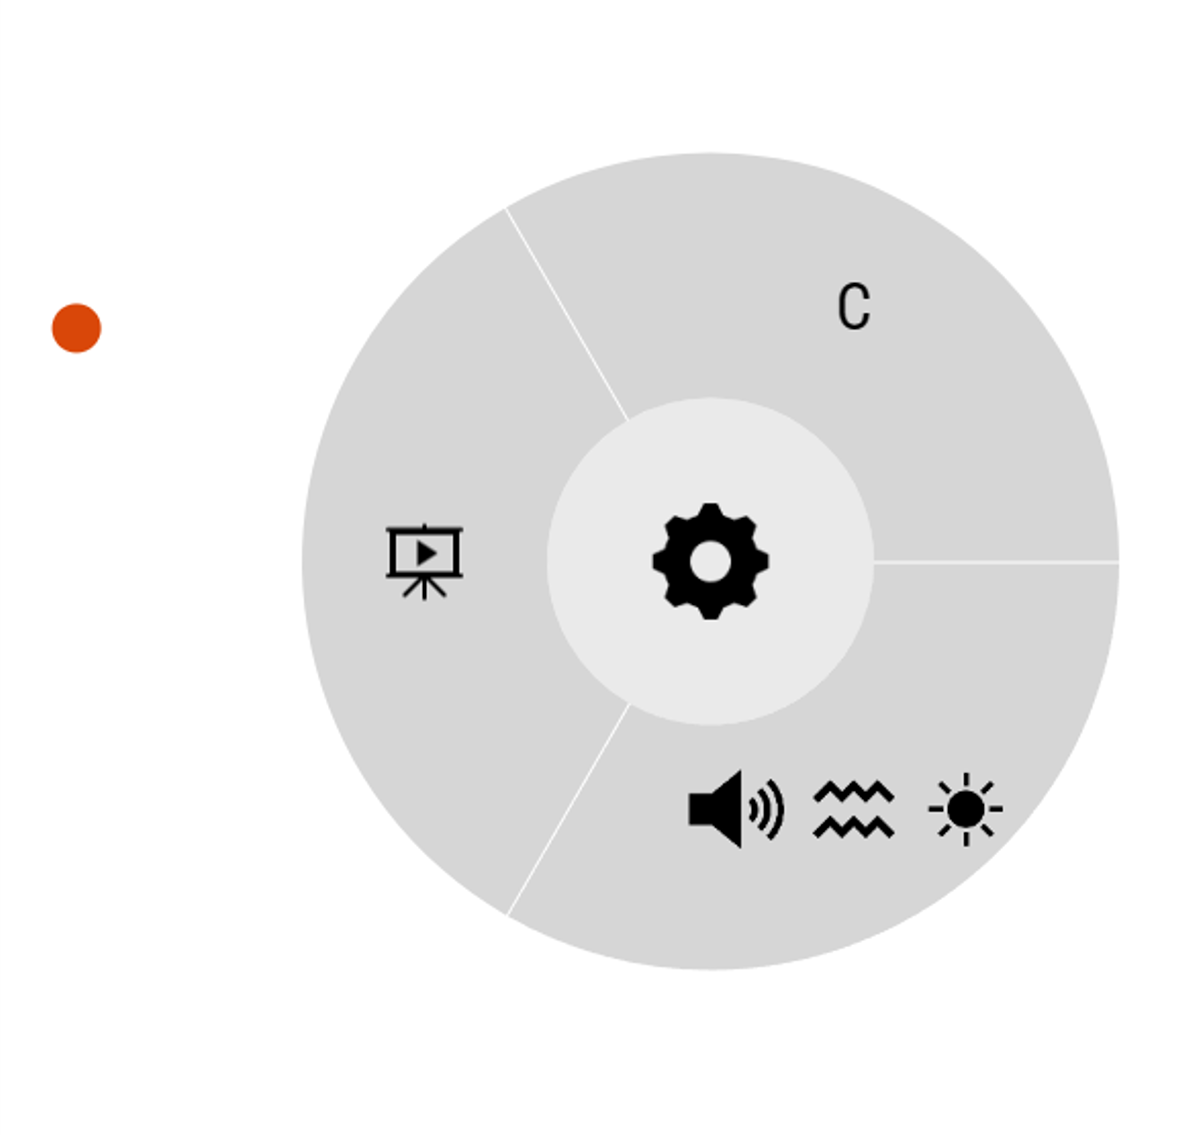
\includegraphics[width=\linewidth]{content/images/menu_cursor3.png}
        \caption{Cursor ist aus Submenü herausnavigiert, woraufhin sich Submenü geschlossen hat.}
        \label{fig:menu_cursor3}
    \end{subfigure}
    \caption{Zustandsdarstellungen der Submenü-Sichtbarkeitslogik {\color{red} Braucht man die Visualisierung oder checkt man das auch ohne?}}
    \label{fig:submenu}
\end{figure}

\subsubsection{Slider}
Während das radiale Menü insbesondere für diskrete Auswahlentscheidungen geeignet ist, erfordern kontinuierliche Parameter wie Lautstärke, Helligkeit oder Vibrationsintensität eine andere Form der Interaktion. Deshalb wurde das menübasierte Konzept um Slider als Mechanismus zur kontinuierlichen Steuerung erweitert.
Diese Erweiterung greift die in Abschnitt~\ref{sec:rw_menus} diskutierte Frage auf, wie Marking-Menu-artige Systeme über reine Befehlsauswahl hinaus auch zur feineren Parametersteuerung genutzt werden können. Das Ziel besteht darin, diskrete und kontinuierliche Interaktion innerhalb eines gemeinsamen Systems zu vereinen, anstatt für unterschiedliche Aufgaben vollständig getrennte Interaktionsparadigmen einzuführen.
Im Kontext des Marking-Menus erfolgt dies durch die Auswahl eines Menüeintrags, der bereits während des Hover-Zustands durch eine visuelle Vorschau auf die veränderte Interaktionsart hinweist (Abb.~\ref{fig:slider_preview}). Die reduzierte visuelle Hervorhebung signalisiert dabei, dass zunächst eine explizite Auswahl des Menüsegments erforderlich ist, um die Sliderinteraktion zu aktivieren. Nach Bestätigung der Auswahl wechselt das System in einen Anpassungsmodus, in dem der Parameter direkt verändert werden kann (Abb.~\ref{fig:slider_active}). In diesem Modus wird das Menü visuell zurückgenommen und der Cursor ausgeblendet, um den Fokus auf die Sliderinteraktion zu lenken.

\begin{figure}[H]
    \centering
    \begin{subfigure}{0.49\textwidth}
        \centering
        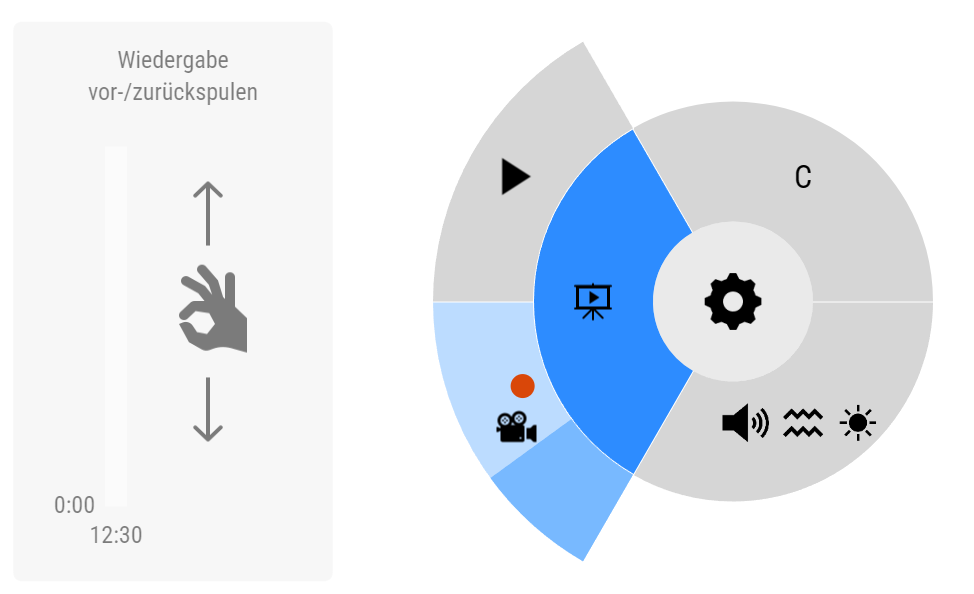
\includegraphics[width=\linewidth]{content/images/menu_with_slider_presentation.png}
        \caption{Vorschau}
        \label{fig:slider_preview}
    \end{subfigure}
    \hfill
    \begin{subfigure}{0.49\textwidth}
        \centering
        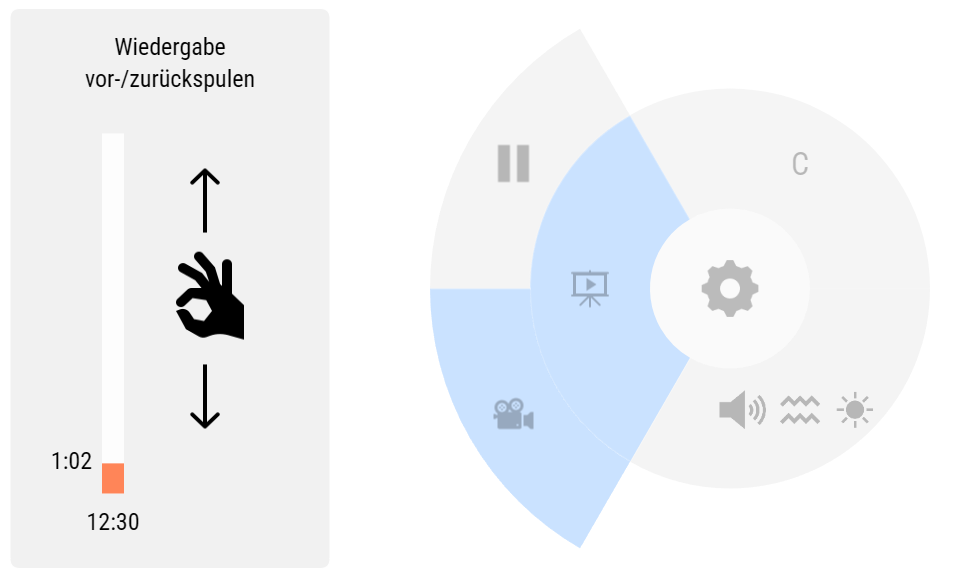
\includegraphics[width=\linewidth]{content/images/slider_active.png}
        \caption{Aktiver Zustand}
        \label{fig:slider_active}
    \end{subfigure}
    \caption{Darstellungen der verschiedenen Slider-Zustände}
    \label{fig:slider_states}
\end{figure}

Die Steuerung erfolgt über eine gezielte Handbewegung entlang einer definierten Interaktionsachse. Diese wird durch eine Pinch-Geste aktiviert, bei der Nutzer:innen den Parameter durch Verschieben der Hand entlang der jeweiligen Achse verändern. Die Kombination aus Aktivierungsgeste und anschließender gerichteter Bewegung greift Elemente von Micro-Gesten-basierten Interaktionen auf (vgl. Abschnitt~\ref{sec:rw_gestures} und Abschnitt~\ref{sec:rw_menus}). Um die Discoverability der Interaktion zu verbessern, wird im Sliderbereich eine visuelle Anleitung eingeblendet, die die Pinch-Geste sowie die mögliche Bewegungsrichtung verdeutlicht. Diese visuelle Unterstützung erleichtert insbesondere Erstnutzer:innen den Einstieg in die Interaktion.

Gleichzeitig greift die Interaktion eine vertraute physische Metapher auf: Das Verschieben des Sliders entspricht dem Greifen und Bewegen eines realen Reglers. Diese räumliche Analogie unterstützt eine intuitive Bedienung und ermöglicht es Nutzer:innen, die Interaktion durch Lösen der Pinch-Geste jederzeit zu beenden, wodurch eine kontrollierte und leicht verständliche Anpassung der Werte entsteht.

\begin{figure}[H]
    \centering
    \begin{subfigure}[t]{0.27\textwidth}
        \centering
        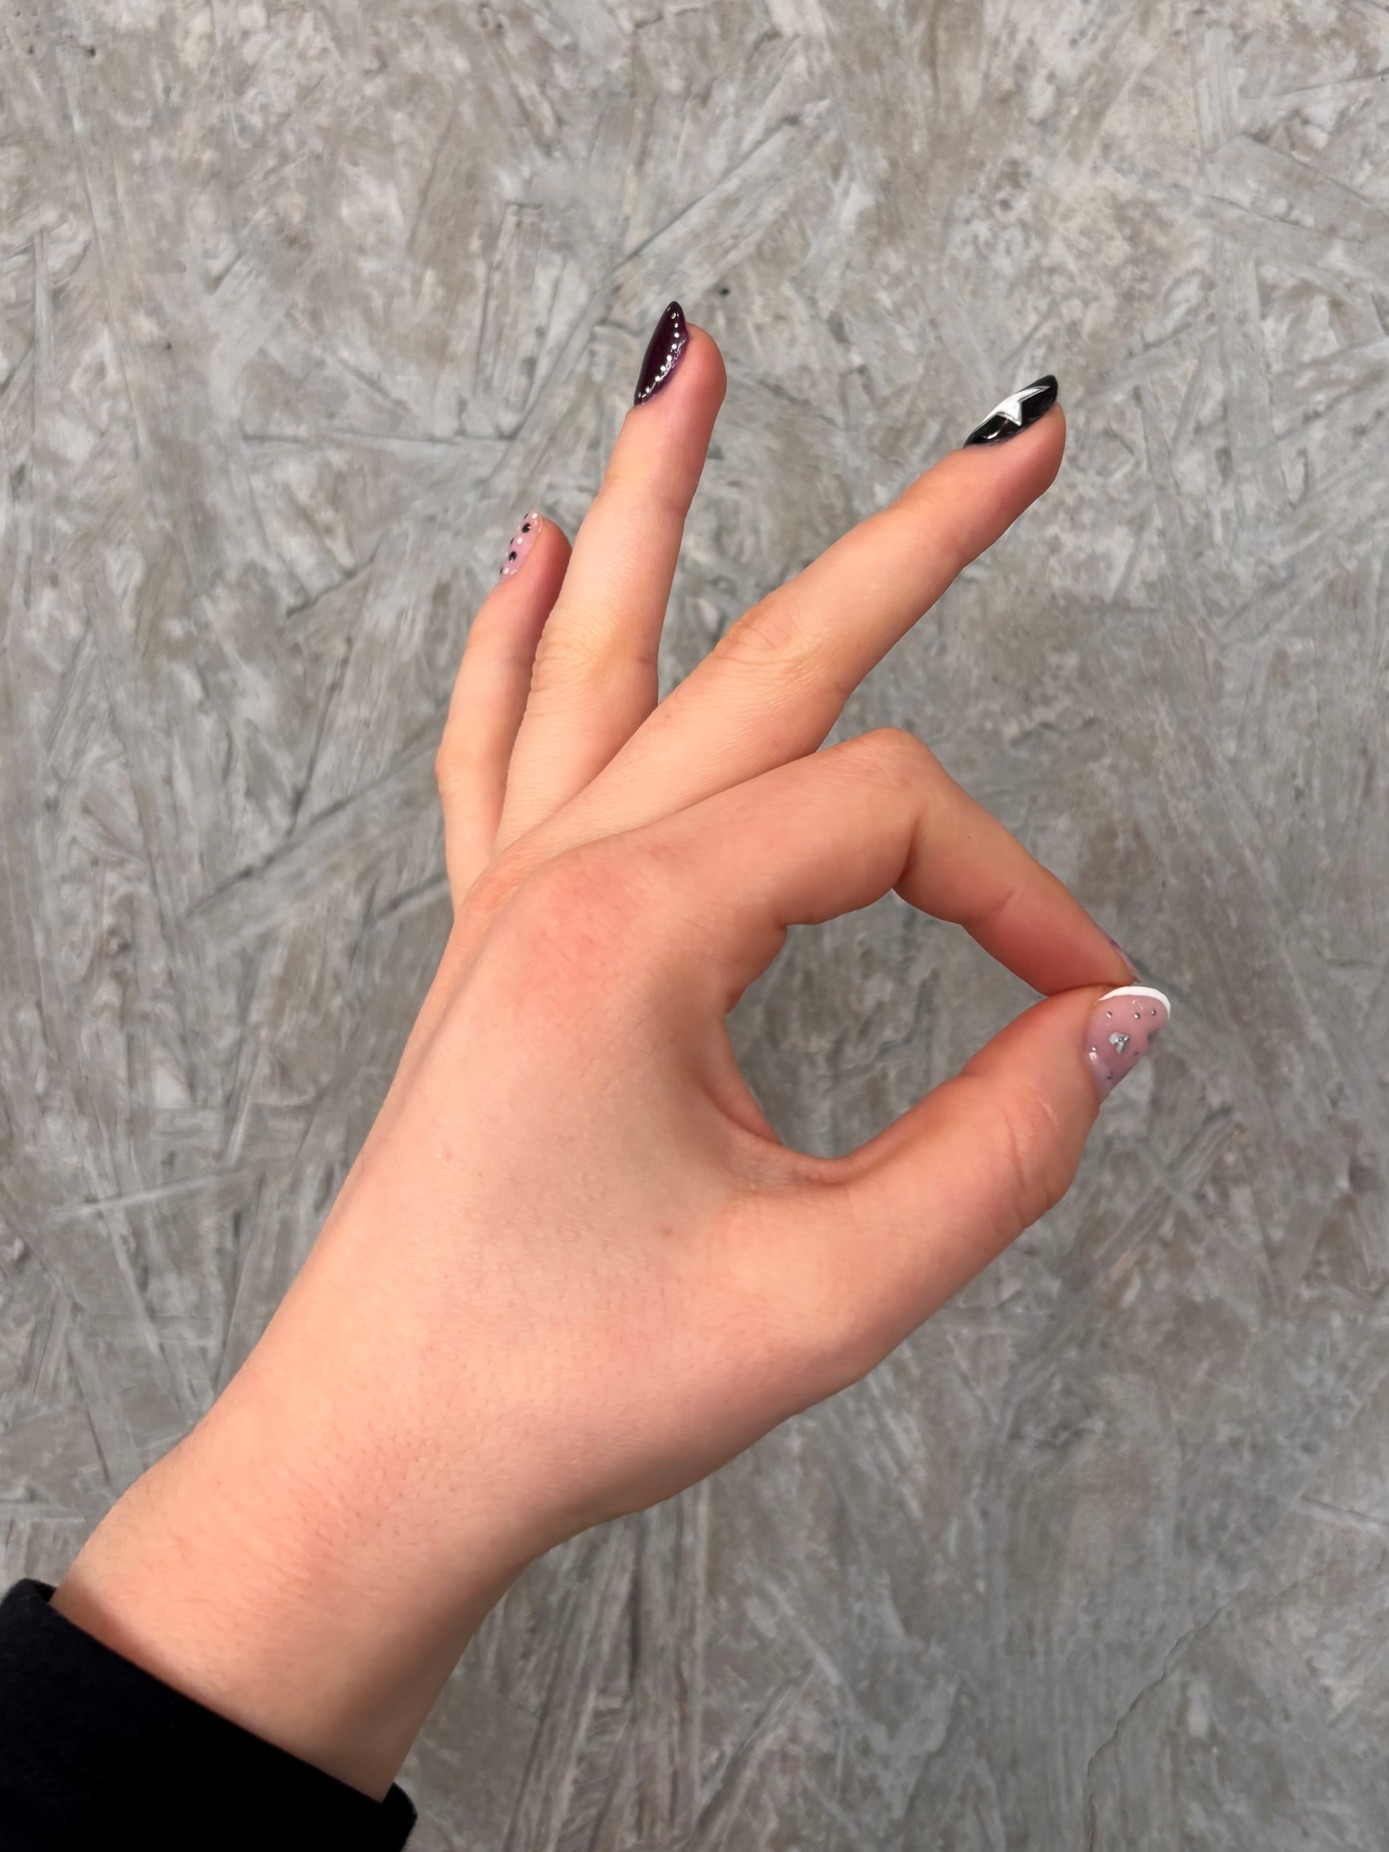
\includegraphics[width=\linewidth]{content/images/pinch_gesture.jpg}
        \caption{Pinch, bei dem aktiv ein Sliderwert verändert wird.}
        \label{fig:pinch_gesture}
    \end{subfigure}
    \hspace{0.5cm}
    \begin{subfigure}[t]{0.27\textwidth}
        \centering
        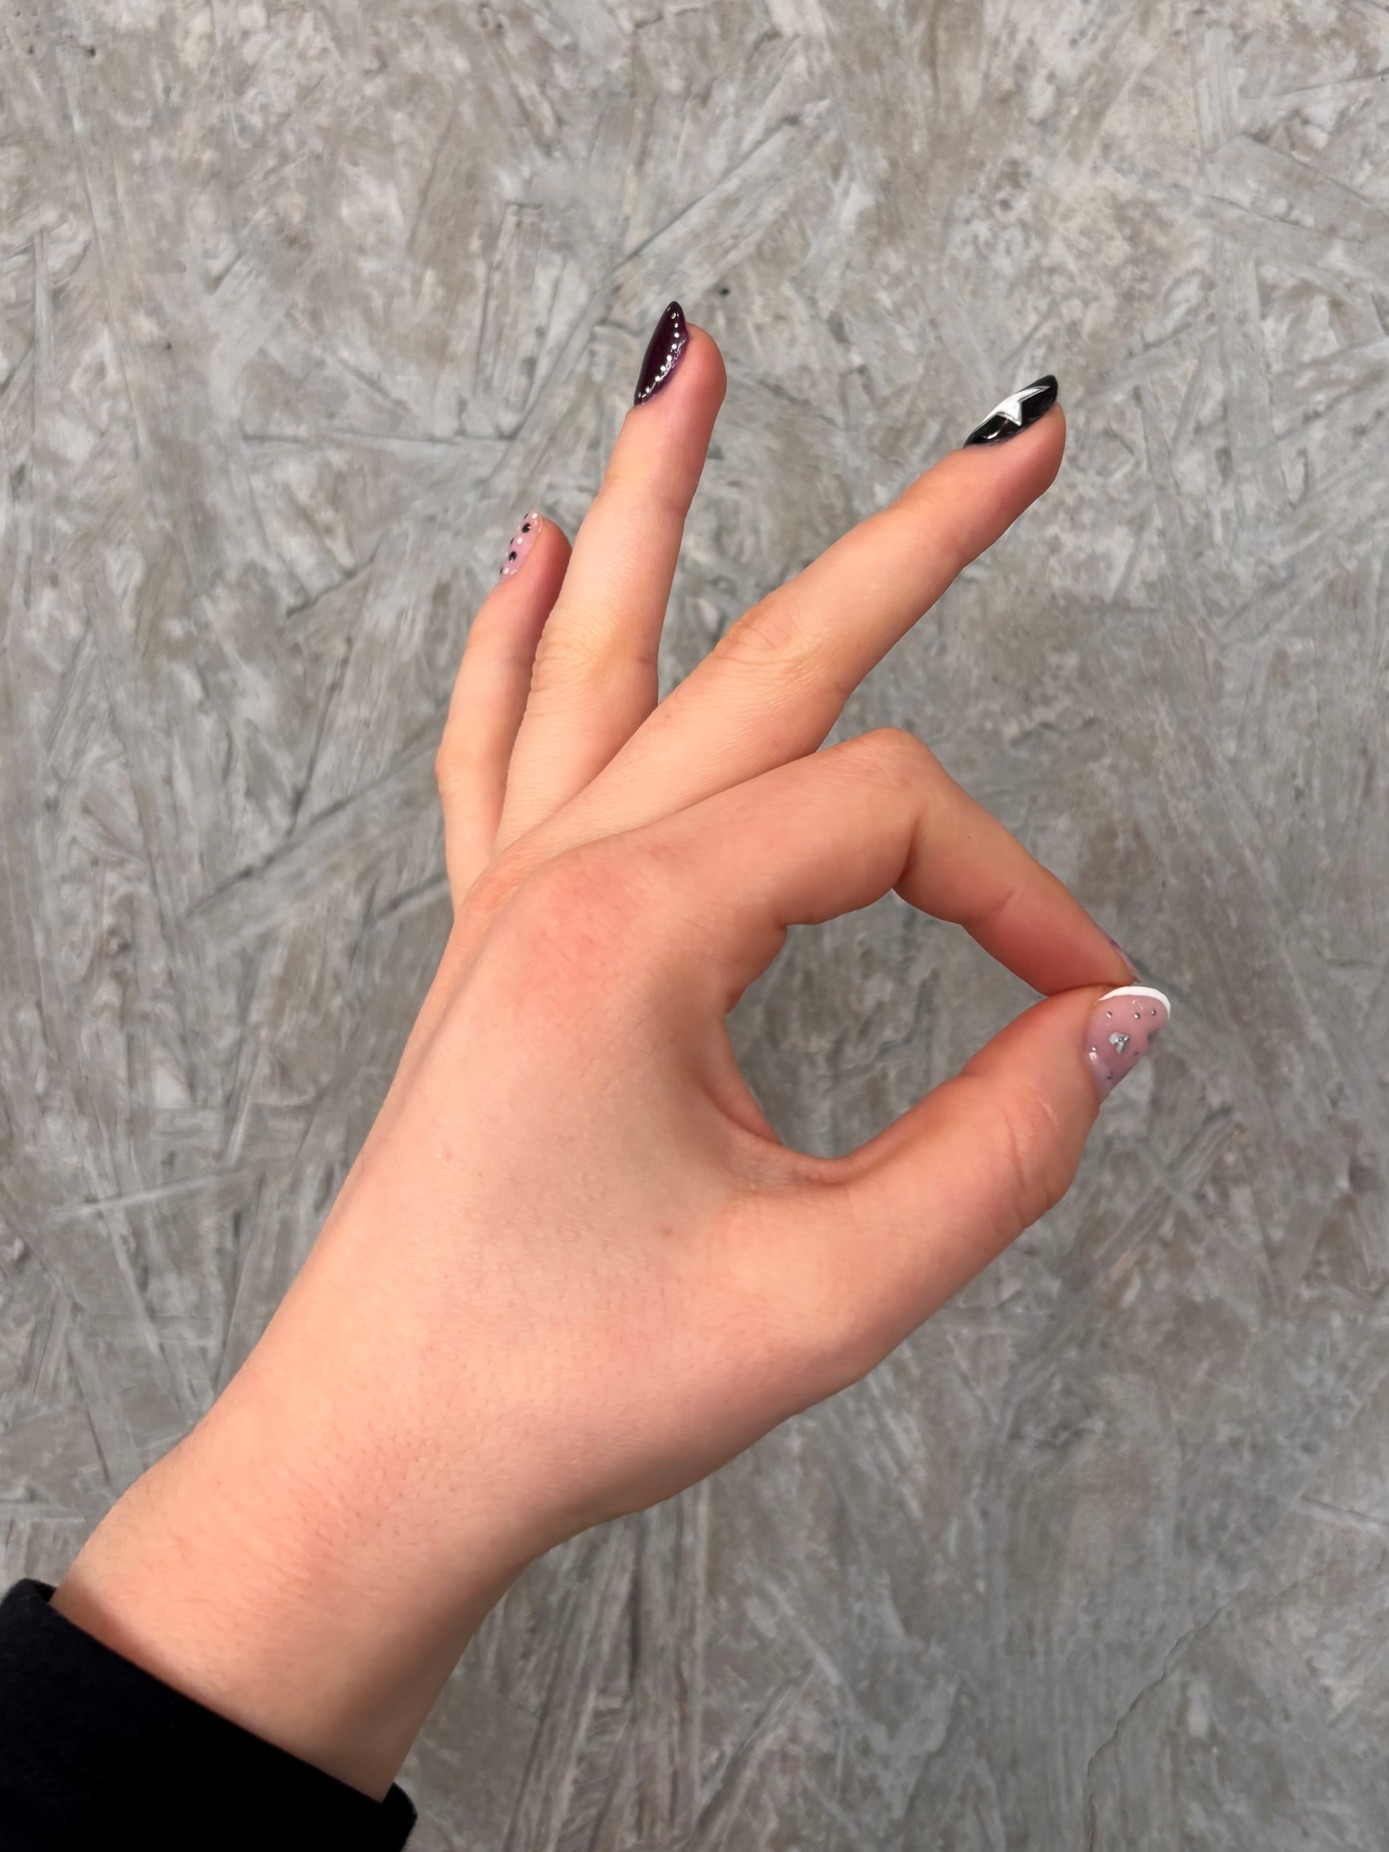
\includegraphics[width=\linewidth]{content/images/pinch_gesture.jpg}
        \caption{Geste, bei der der Sliderwert nicht aktiv verändert wird. {\color{red} TODO Foto von offenem Pinch machen!!}}
        \label{fig:pinch_gesture_open}
    \end{subfigure}
    \caption{Darstellungen der verschiedenen Pinch-Gestenzustände}
    \label{fig:pinch}
\end{figure}

Je nach Kontext und Menüeintrag wird die Position des Sliders relativ zum Menü angepasst. Der Slider kann dabei oberhalb, unterhalb oder seitlich des Menüs erscheinen, wodurch sich entweder eine horizontale oder vertikale Interaktionsachse ergibt. Entsprechend wird die Pinch-Geste entlang dieser Achse ausgeführt, sodass eine konsistente räumliche Zuordnung zwischen visueller Darstellung und Interaktionsbewegung entsteht.

Durch die Integration solcher Slider lassen sich kontinuierliche Parameter innerhalb des Interaktionssystems einheitlich steuern.


\subsubsection{Beispiele aktueller Interaktionen}
{\color{red} TODO: überlegen ob button doch in extra abschnitt muss, aber denke eigentlich nicht, weil es gibt ja nur den einen => dann eher generalisierbarkeit als todo in den ausblick }

Die Marking-Menu Interaktionen umfassen sowohl kontinuierliche Parametersteuerungen als auch diskrete Steuerungsfunktionen.
Ein zentraler Anwendungsfall für kontinuierliche Interaktion sind Slider zur Anpassung von Parametern wie Helligkeit, Vibration und Lautstärke. Diese werden in Form prozentualer Werte dargestellt und ermöglichen eine direkte, kontinuierliche Kontrolle der jeweiligen Systemparameter.

Darüber hinaus wird das Interaktionssystem zur Steuerung vorgerenderter Medieninhalte eingesetzt. In diesem Kontext dient ein Slider zur Navigation innerhalb eines Videos, indem er die aktuelle Abspielposition repräsentiert und gleichzeitig die Gesamtlänge des Materials visualisiert. Während der Wiedergabe bewegt sich der Slider automatisch entlang der Zeitleiste, wodurch der aktuelle Fortschritt kontinuierlich angezeigt wird.

Abbildung~\ref{fig:Slidertypen} zeigt beide Varianten im Vergleich. Während parameterbasierte Slider den aktuellen Wert als prozentuale Angabe darstellen, repräsentieren medienbezogene Slider eine zeitliche Position innerhalb eines Videos. Die zugrunde liegende Interaktionslogik bleibt dabei identisch.

\begin{figure}[H]
    \centering
    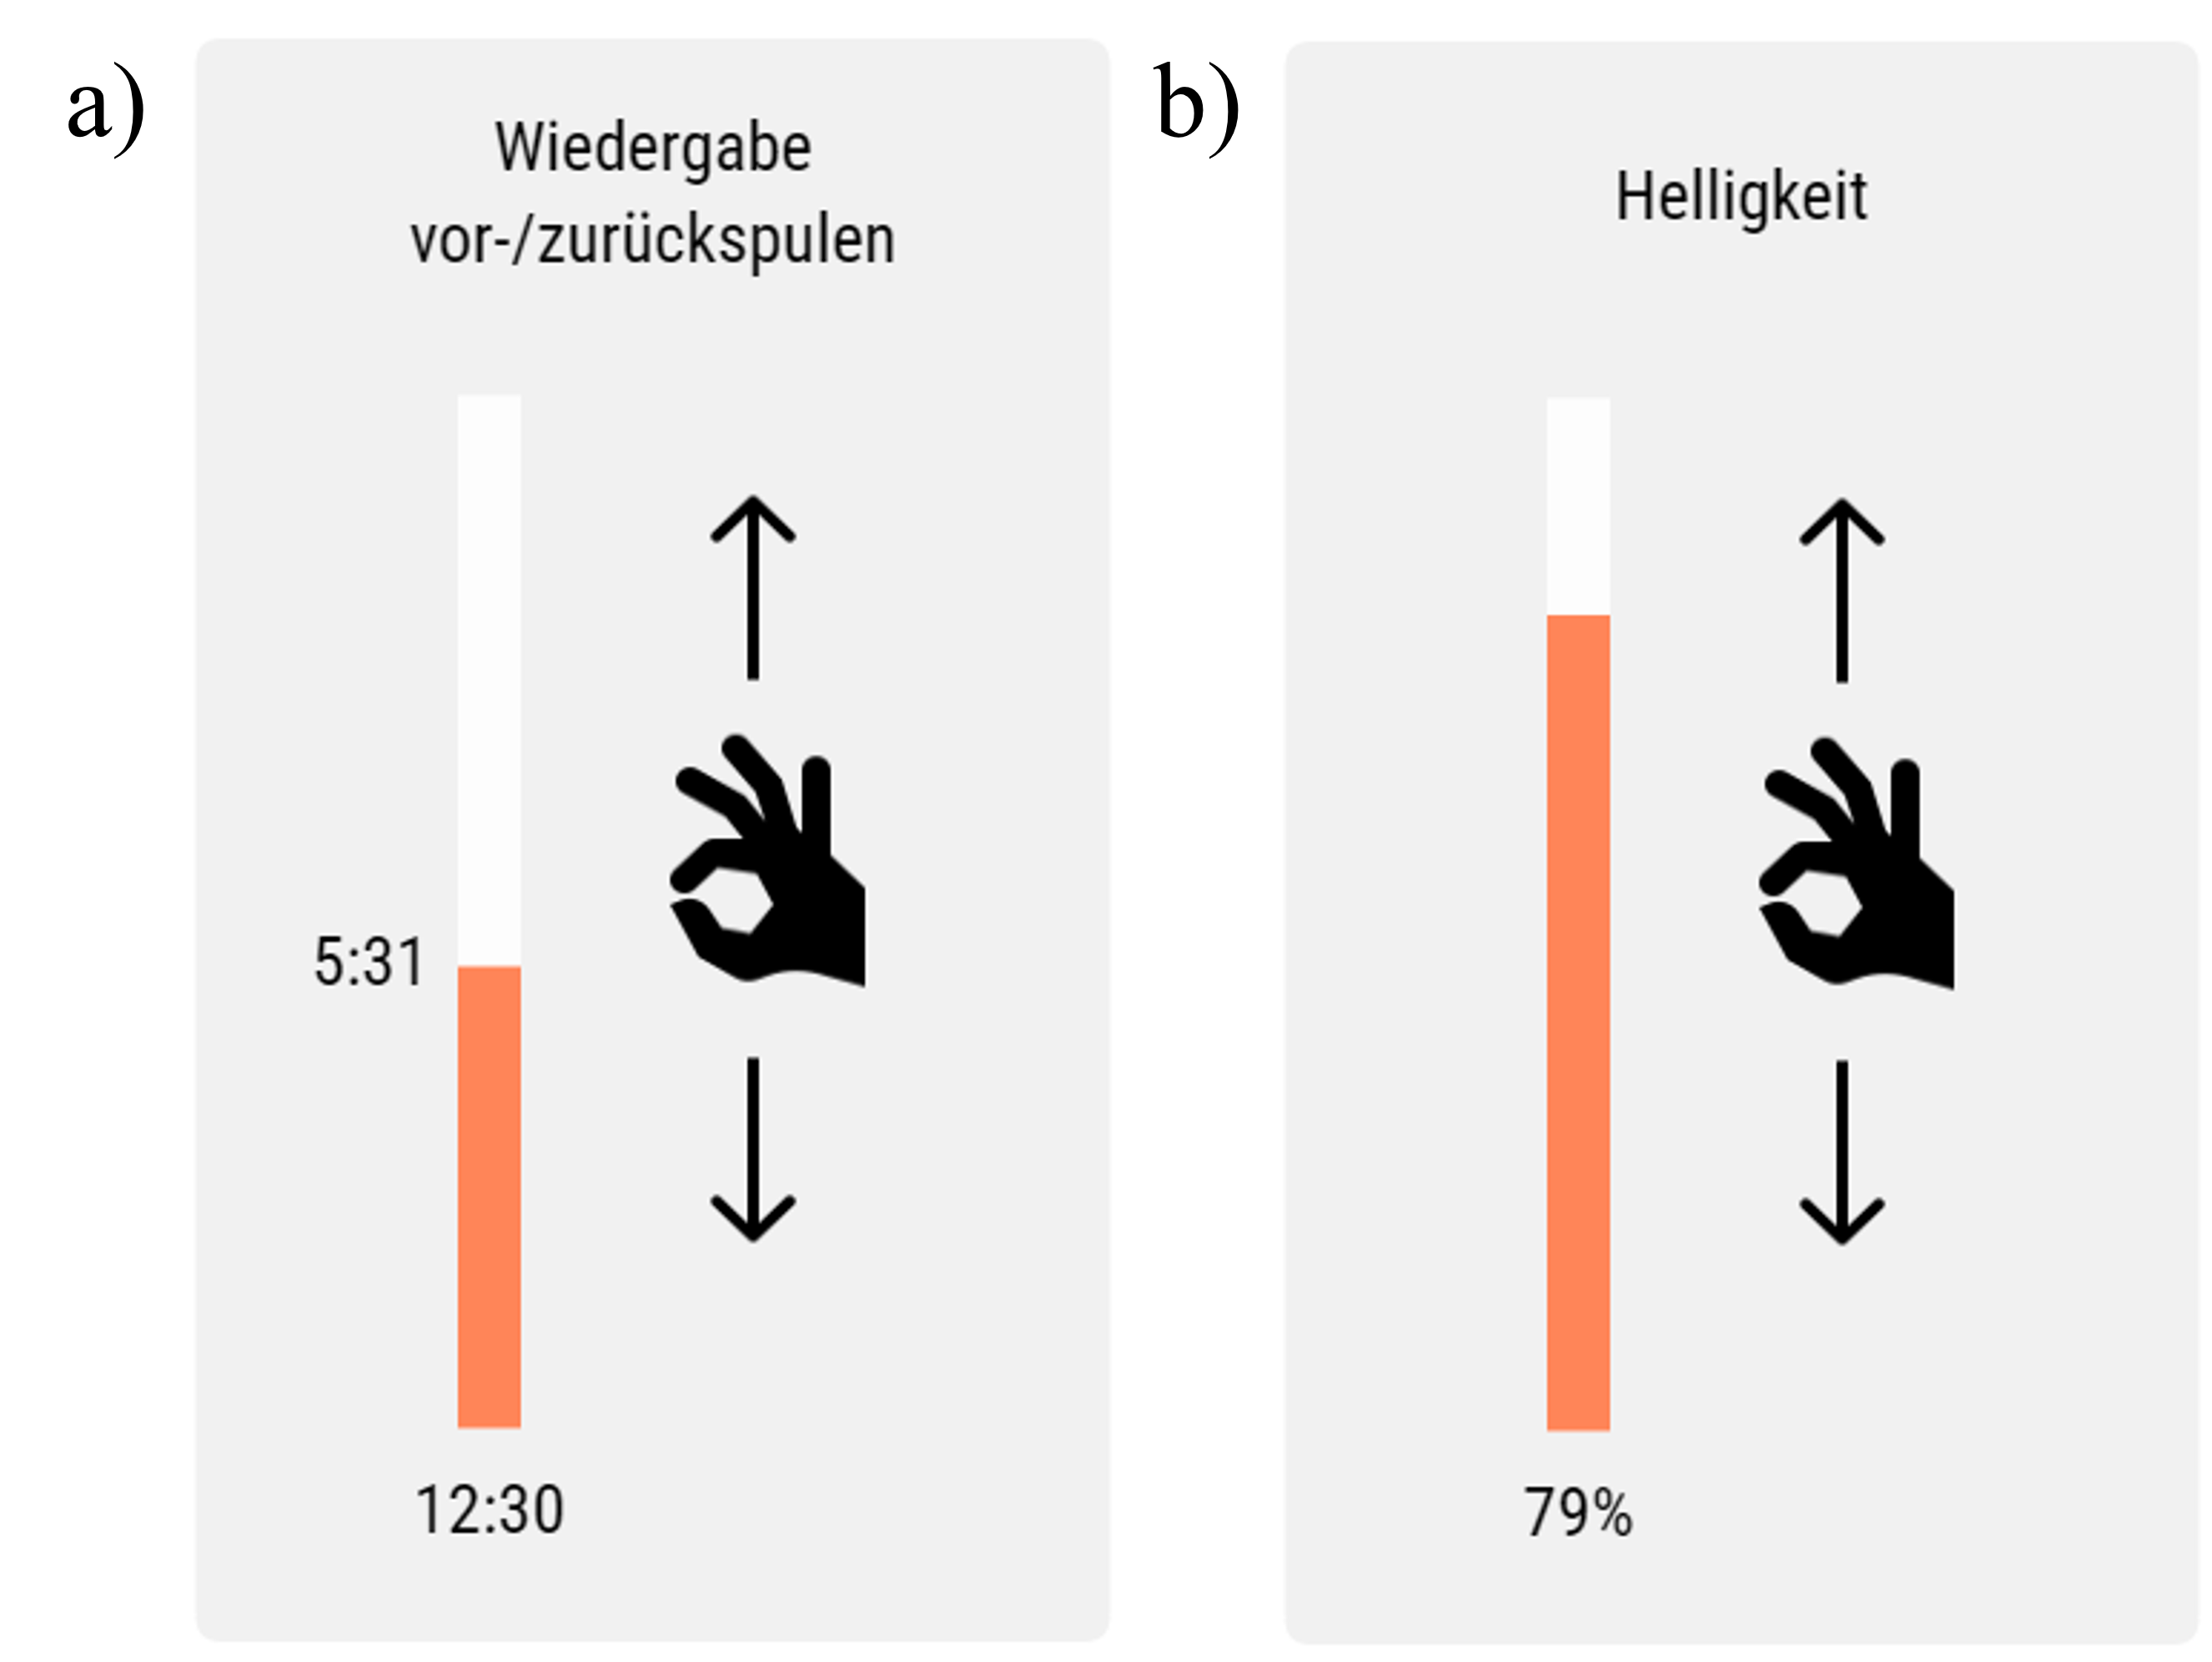
\includegraphics[width=0.5\linewidth]{content/diagrams/Slidertypen.png}
    \caption{Vergleich zweier Slider-Typen: a) zeigt einen zeitbasierten Slider zur Navigation innerhalb eines Videos, b) zeigt einen parameterbasierten Slider mit prozentualer Anzeige. Beide verwenden identische Interaktionsmechanismen bei unterschiedlicher semantischer Bedeutung.}    \label{fig:Slidertypen}
\end{figure}

Ergänzend dazu ist ein Button zur Steuerung der Wiedergabe implementiert, der als klickbares Menüelement realisiert ist. Dieser ermöglicht das Starten und Pausieren von Videomaterial. Der aktuelle Systemzustand wird dabei durch eine visuelle Änderung des Icons kommuniziert, wie in Abbildung \ref{fig:Buttons} dargestellt. Der Button kann wiederholt aktiviert werden und verhält sich funktional analog zu einem klassischen physischen Bedienelement, ist jedoch in die Menüstruktur integriert.

\begin{figure}[H]
    \centering
    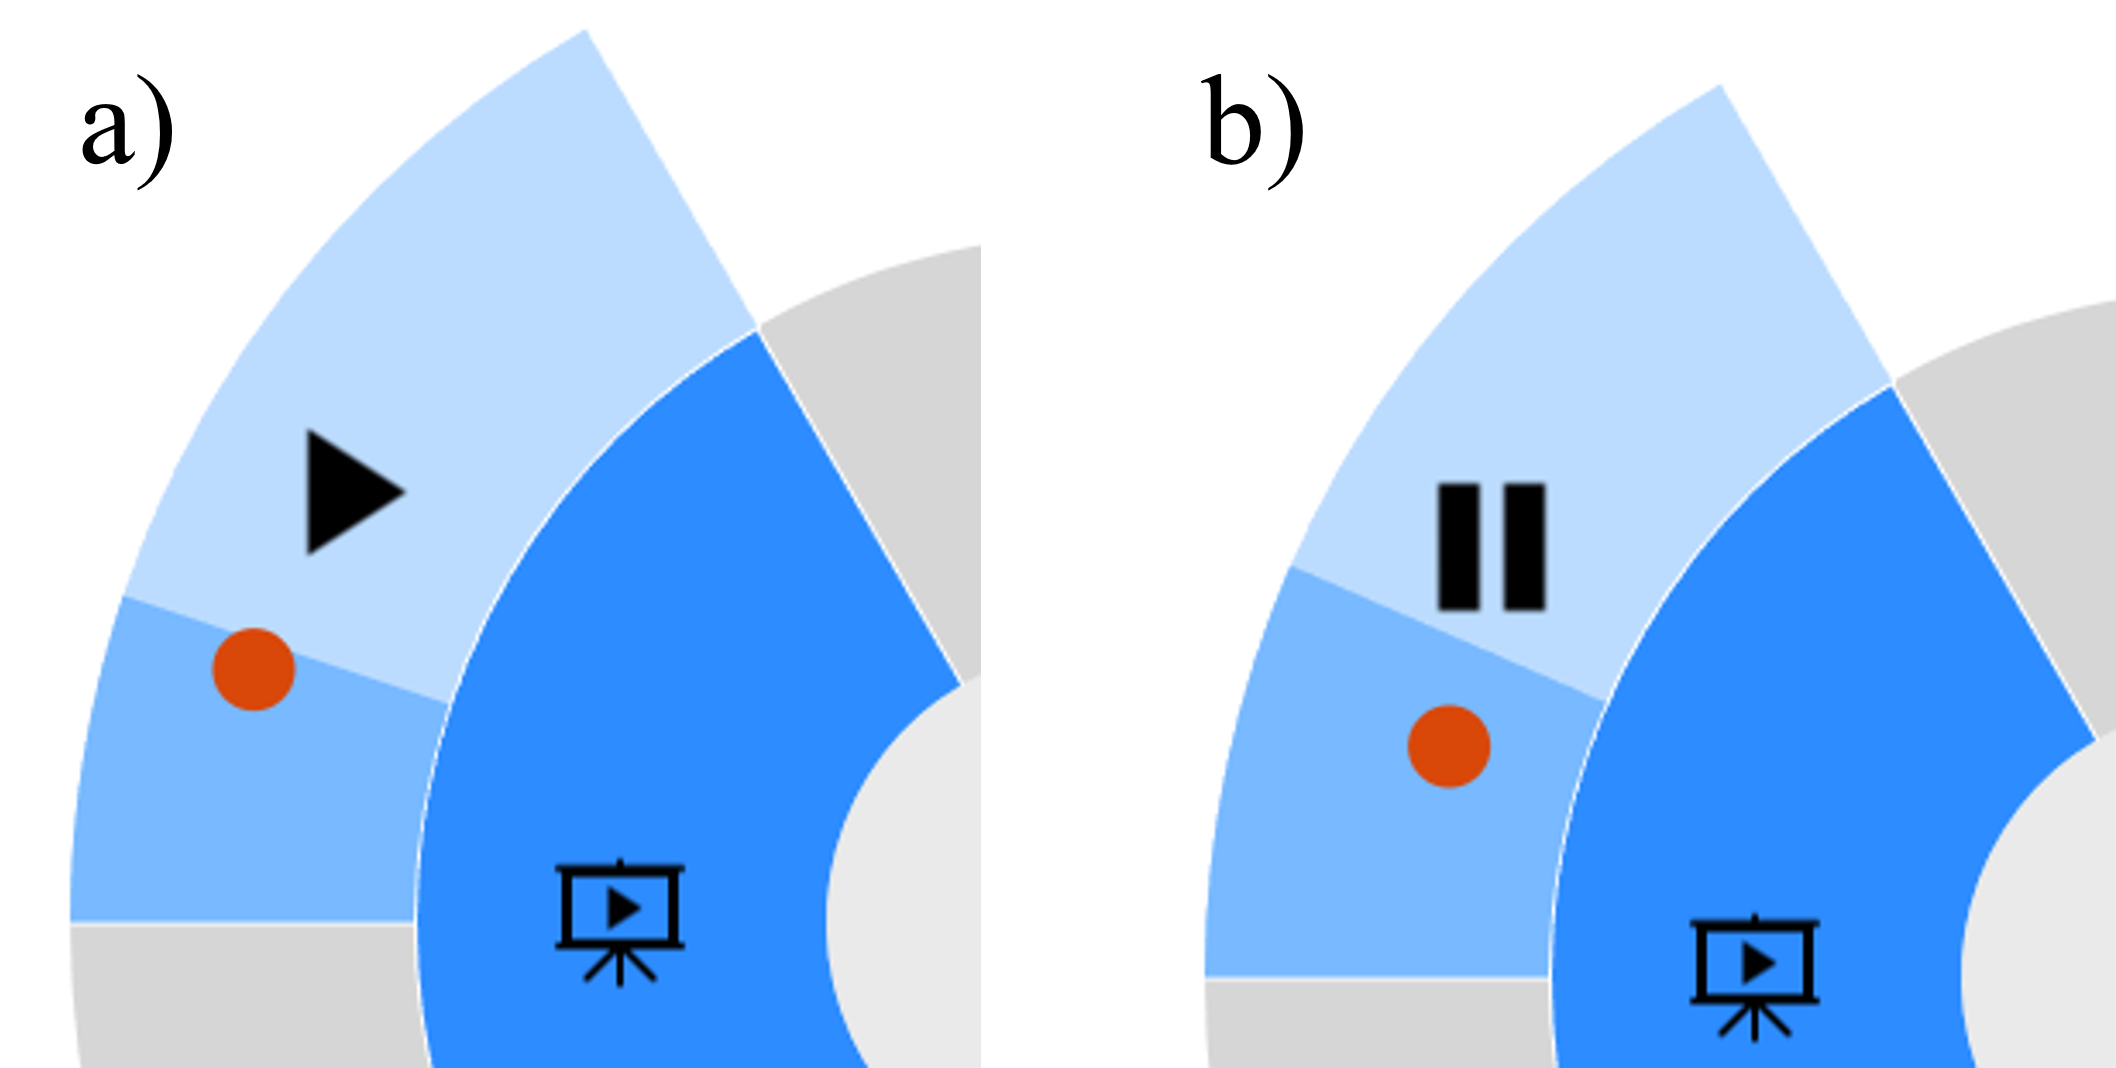
\includegraphics[width=0.5\linewidth]{content/diagrams/Buttons.png}
    \caption{Darstellung der beiden Buttonzustände. a) zeigt den Button, während das Video pausiert ist, b) zeigt den Button, während das Video läuft.}
    \label{fig:Buttons}
\end{figure}

        {\color{red} Muss man für so einen Abschlusssatz ein Zusammenfassungsunterkapitel machen oder ist das ok, wenn das einfach bei Slider mit drin steht? }
% Überagang
Das beschriebene Interaktionskonzept kombiniert somit gestenbasierte Eingaben mit einer strukturierten Menüoberfläche. Durch die Kombination aus radialem Menü, hierarchischen Untermenüs und kontinuierlichen Steuerungselementen können unterschiedliche Interaktionsaufgaben innerhalb eines einheitlichen Systems abgebildet werden. Gleichzeitig bleibt die Interaktion vollständig controllerlos und in den räumlichen Kontext des MIR integriert.


\clearpage
\section{Praktische Umsetzung}

% Einleitung ins Kapitel
Auf Grundlage der im Abschnitt \ref{sec:analyse} durchgeführten Analyse bestehender Szenarien sowie der Auseinandersetzung mit verwandten Arbeiten wurde ein gestenbasiertes Marking-Menu als zentrales Interaktionsparadigma ausgewählt und im Abschnitt \ref{sec:synthese} konzeptionell ausgearbeitet. Dieses Kapitel beschreibt nun die praktische Umsetzung dieses Konzepts. Im Vordergrund steht dabei nicht eine spezifische Zielanwendung, sondern ein generisches System, das als zusätzliche Interaktionsschicht über bestehende Anwendungen gelegt werden kann. Die Implementierung wurde daher so aufgebaut, dass Benutzungsoberfläche und Anwendungsanbindung voneinander getrennt sind. Dadurch kann das System unabhängig entwickelt, getestet und prinzipiell in verschiedene Anwendungskontexte integriert werden.
Zur Veranschaulichung der prototypischen Umsetzung im realen Nutzungskontext zeigt Abbildung~\ref{fig:photos_mir} exemplarische Interaktionssituationen im Multisensorischen Interaktionsraum.

\begin{figure}[H]
    \centering
    \begin{subfigure}[t]{0.32\textwidth}
        \centering
        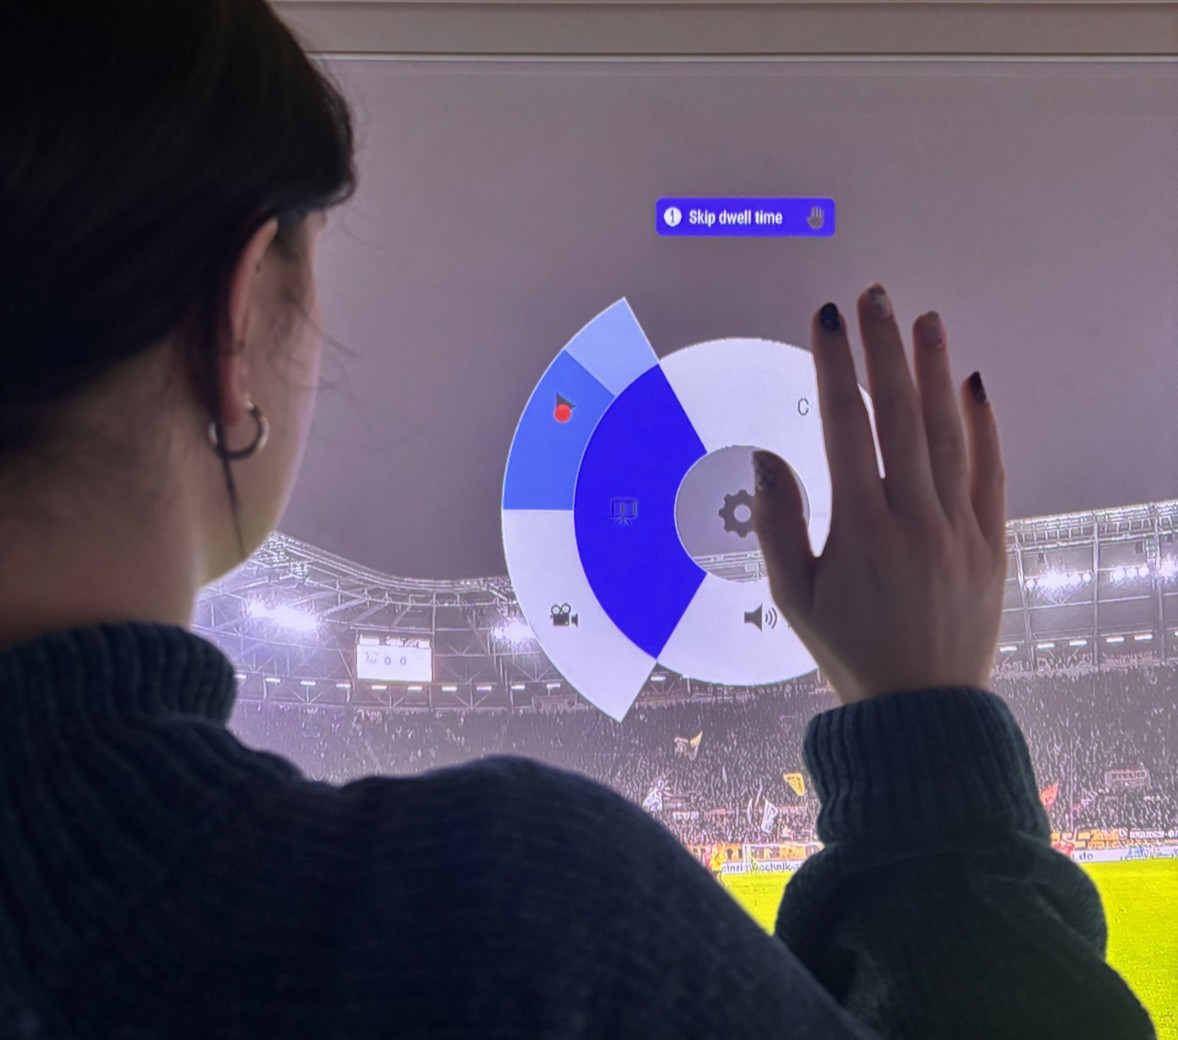
\includegraphics[width=\linewidth]
        {content/images/photo_mir1.jpg}
        \caption{Nutzerin hovert Play Button.}
        \label{fig:photo_mir1}
    \end{subfigure}
    \hfill
    \begin{subfigure}[t]{0.32\textwidth}
        \centering
        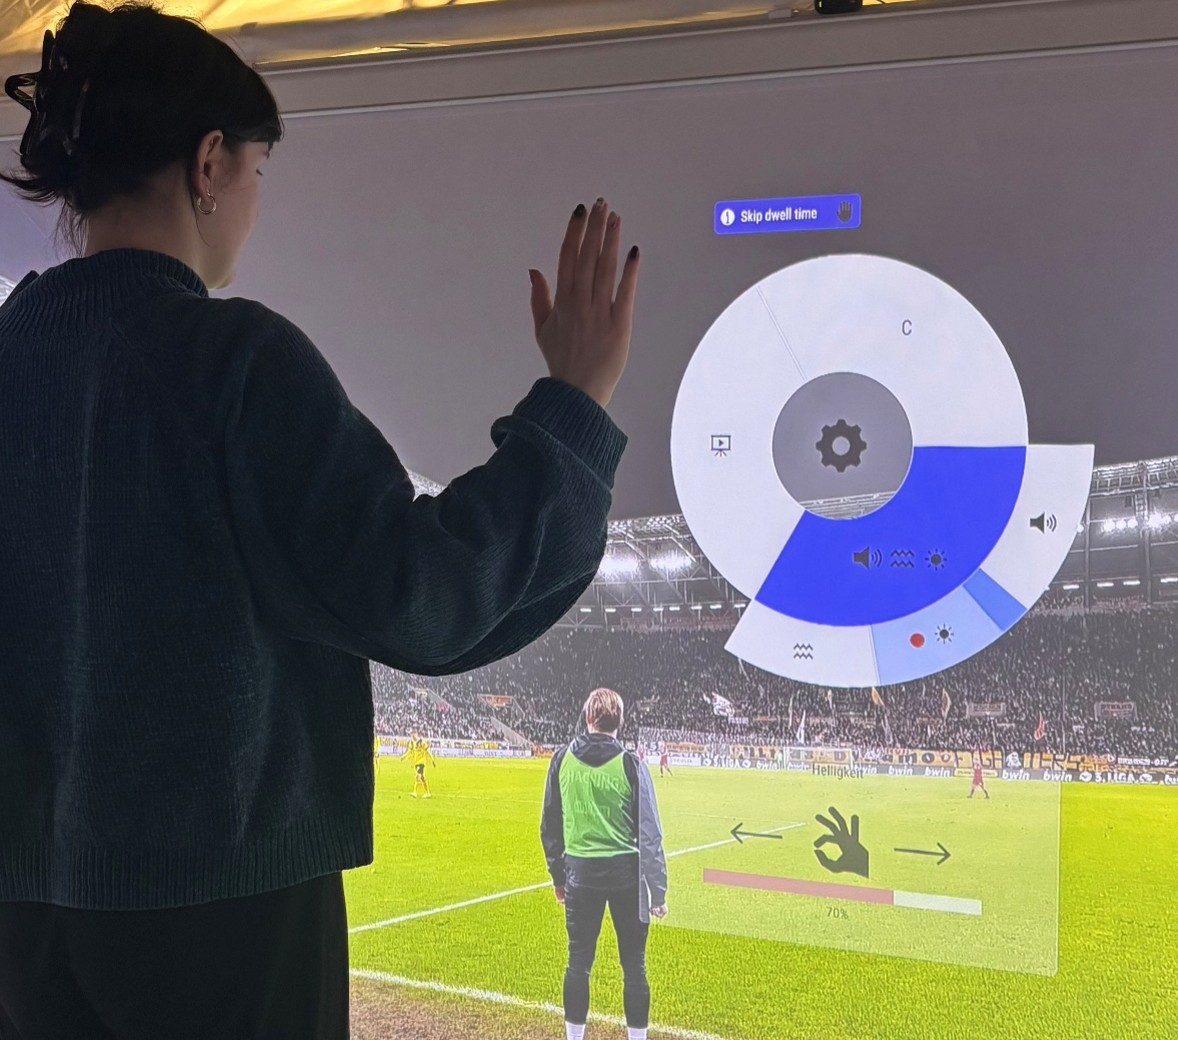
\includegraphics[width=\linewidth]
        {content/images/photo_mir2.jpg}
        \caption{Nutzerin öffnet Vorschau für Helligkeitsslider.}
        \label{fig:photo_mir2}
    \end{subfigure}
    \hfill
    \begin{subfigure}[t]{0.32\textwidth}
        \centering
        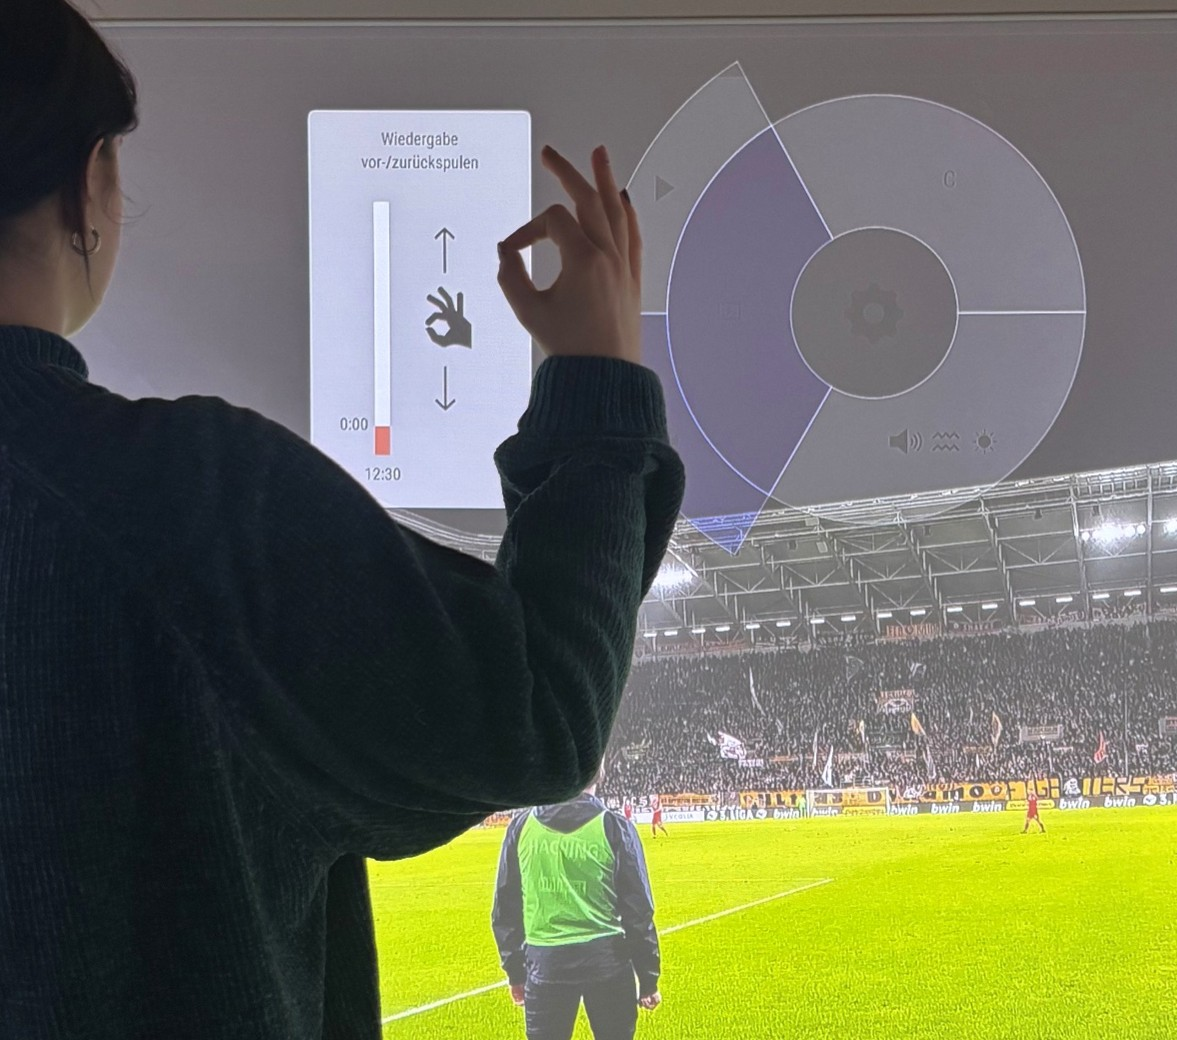
\includegraphics[width=\linewidth]
        {content/images/photo_mir3.jpg}
        \caption{Nutzerin manipuliert Wiedergabezeitpunkt.}
        \label{fig:photo_mir3}
    \end{subfigure}
    \caption{Nutzerin modifiziert Einstellung mit Hilfe von Marking-Menu im MIR. Das ausgewählte Szenario ist das Fußballstadion.}
    \label{fig:photos_mir}
\end{figure}


\subsection{Systemarchitektur}
Die Systemarchitektur basiert auf einer Verarbeitungspipeline, die in eine modulare Frontend-Struktur eingebettet ist. Aus den Kameradaten werden zunächst Handmerkmale extrahiert. Auf Basis dieser Tracking-Daten wird eine Cursorposition im zweidimensionalen Interaktionsraum berechnet. Diese steuert die Benutzungsoberfläche des Systems, die das Marking-Menu sowie weitere Interaktionselemente darstellt.
Aktionen, die aus der Menüinteraktion entstehen, werden anschließend über eine WebSocket-Schnittstelle an eine angebundene Zielanwendung übertragen.
Abbildung~\ref{fig:handtracking_pipeline_diagram} zeigen die grundlegenden Komponenten der Verarbeitungspipeline des Systems von der Kameradatenerfassung bis zur Übertragung der Interaktionsereignisse an die Zielanwendung.

\begin{figure}[htbp]
    \centering
    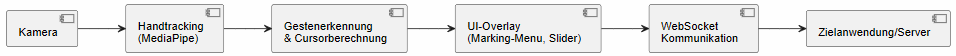
\includegraphics[width=0.99\linewidth]{content/diagrams/handtracking_pipeline_diagram.png}
    \caption{Komponenten der Verarbeitungspipeline des Interaktionssystems}
    \label{fig:handtracking_pipeline_diagram}
\end{figure}

Die Kommunikation zwischen Interaktionssystem und Zielanwendung erfolgt über WebSocket. 
WebSocket ist ein Netzwerkprotokoll, das eine persistente, bidirektionale Kommunikationsverbindung zwischen Client und Server über eine einzelne TCP-Verbindung ermöglicht \parencite{fetteMelnikov2011TheWebsocketProtocol}. Dadurch können Ereignisse in Echtzeit übertragen werden, ohne dass wiederholt neue HTTP-Verbindungen aufgebaut werden müssen.

Neben dieser linearen Verarbeitungskette ist das System in mehrere funktionale Komponenten unterteilt, die innerhalb des Frontends zusammenwirken:
\begin{itemize}
    \item eine Handtracking-Komponente zur Extraktion von Handlandmarken aus Kameradaten,
    \item eine Gestenerkennung und Cursorberechnung zur Ableitung von Interaktions\-zuständen,
    \item ein Datenmodell zur Verwaltung von Menüstruktur und Zustandsinformationen,
    \item eine UI-Steuerung mit Rendering-Komponente zur Darstellung des Marking-Menus und der Interaktionselemente,
    \item sowie eine WebSocket-Kommunikation zur Anbindung externer Zielanwendungen.
\end{itemize}

Abbildung~\ref{fig:component_diagram} zeigt diese Komponenten sowie deren Interaktionen innerhalb des Systems.

\begin{figure}[htbp]
    \centering
    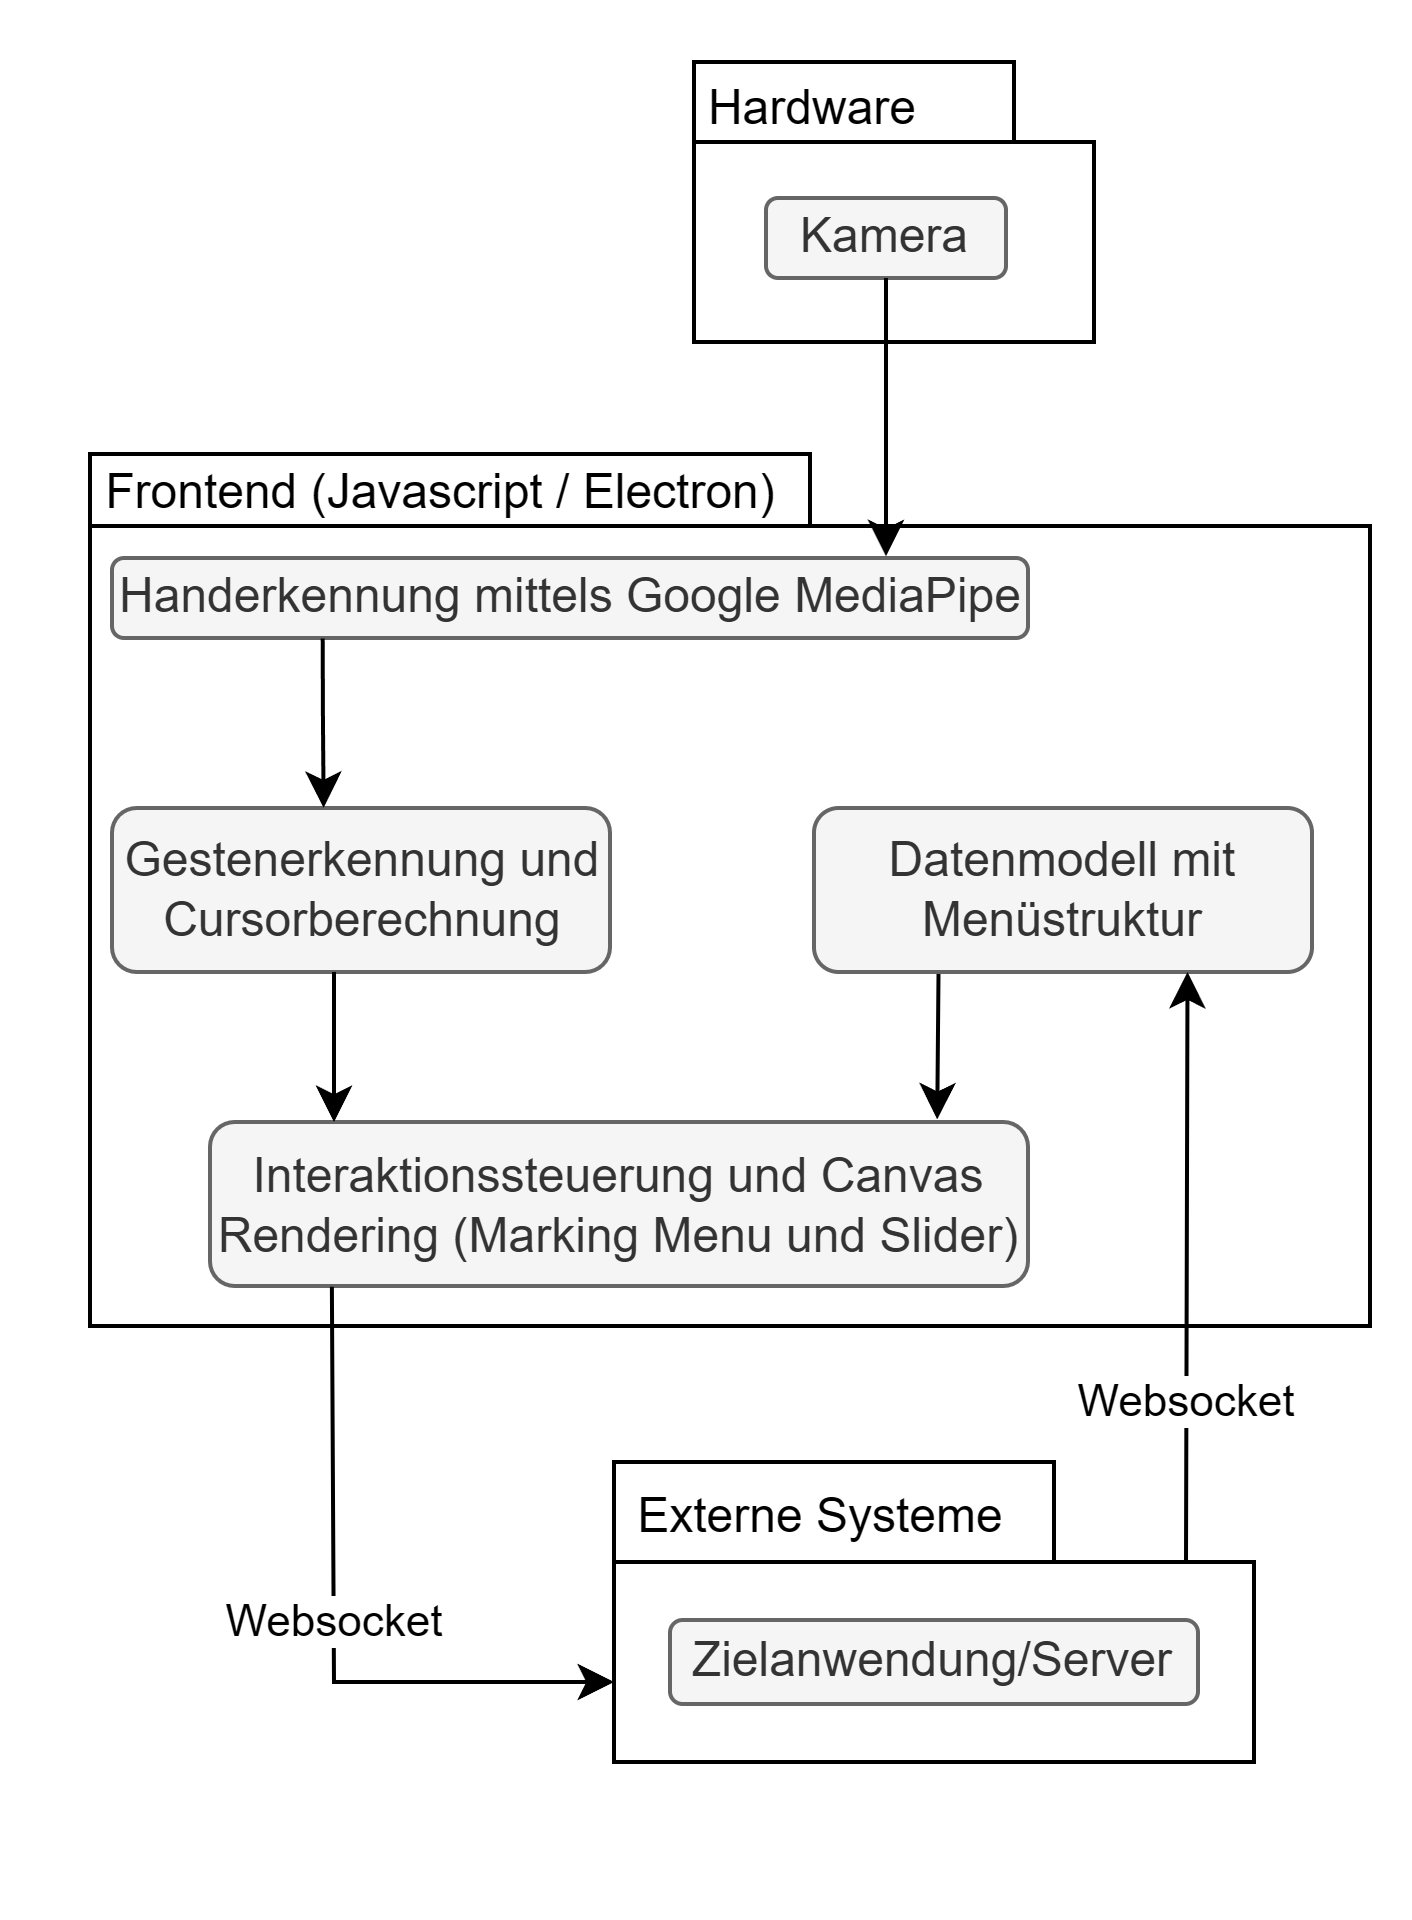
\includegraphics[width=0.8\linewidth]{content/diagrams/component_diagram.png}
    \caption{Vereinfachte Architektur des Interaktionssystems}
    \label{fig:component_diagram}
\end{figure}

Die über WebSocket übermittelten Interaktionsereignisse werden von einer angebundenen Zielanwendung empfangen und verarbeitet. 
Diese Anwendung ist nicht Bestandteil des eigentlichen Interaktionssystems, sondern stellt die Umgebung dar, in der die Interaktionen verarbeitet werden.

Im Kontext des multisensorischen Interaktionsraums wird hierfür typischerweise die \textit{Unreal Engine} verwendet, eine Echtzeit-3D-Engine zur Darstellung und Steuerung der projizierten Inhalte.
Da die Kommunikation jedoch über eine standardisierte Schnittstelle erfolgt, kann das Interaktionssystem prinzipiell mit unterschiedlichen Anwendungen kombiniert werden. 
Dieses Vorgehen unterstützt den Anspruch, das System universell einsetzbar und nicht auf ein einzelnes Anwendungsszenario beschränkt zu gestalten (siehe R2 in Tabelle \ref{tab:requirements}).


\subsection{Handtracking-Pipeline}
\label{sec:handtracking-pipeline}
Die Handtracking-Pipeline bildet die Grundlage des gesamten Interaktionssystems. Ziel ist es, aus dem Kamerabild robuste Informationen über die Position und Form der Hand zu gewinnen und daraus Interaktions\-zustände abzuleiten. Die Implementierung basiert auf einer browsernahen Verarbeitung, sodass die erkannten Handdaten direkt für die visuelle und funktionale Steuerung des Interaktionssystems genutzt werden können.

Zunächst erfasst das System fortlaufend Videoframes der Kamera und übergibt diese an die Handtracking-Komponente \textit{Google MediaPipe}. MediaPipe ist ein Open-Source-Framework zur Echtzeitverarbeitung visueller Sensordaten und stellt vortrainierte Modelle zur Erkennung von Körper-, Gesichts- und Handlandmarken bereit \parencite{lugaresi2019GoogleMediaPipe}. Für jede erkannte Hand liefert das verwendete \textit{MediaPipe Hands Model} 21 dreidimensionale Landmarken, welche die räumliche Lage relevanter Handpunkte beschreiben (siehe Abbildung \ref{fig:mediapipe}).
MediaPipe wurde gewählt, da das Framework eine robuste Echtzeiterkennung von Handlandmarken ermöglicht und direkt in browserbasierten Anwendungen eingesetzt werden kann, wodurch sich die Trackingdaten ohne zusätzliche Verarbeitungsschritte in das Interaktionssystem integrieren lassen.
Auf Basis dieser Landmarken bestimmt das System, ob eine Hand erkannt wurde und welche grundlegende Handhaltung vorliegt.

\begin{figure}[H]
    \centering
    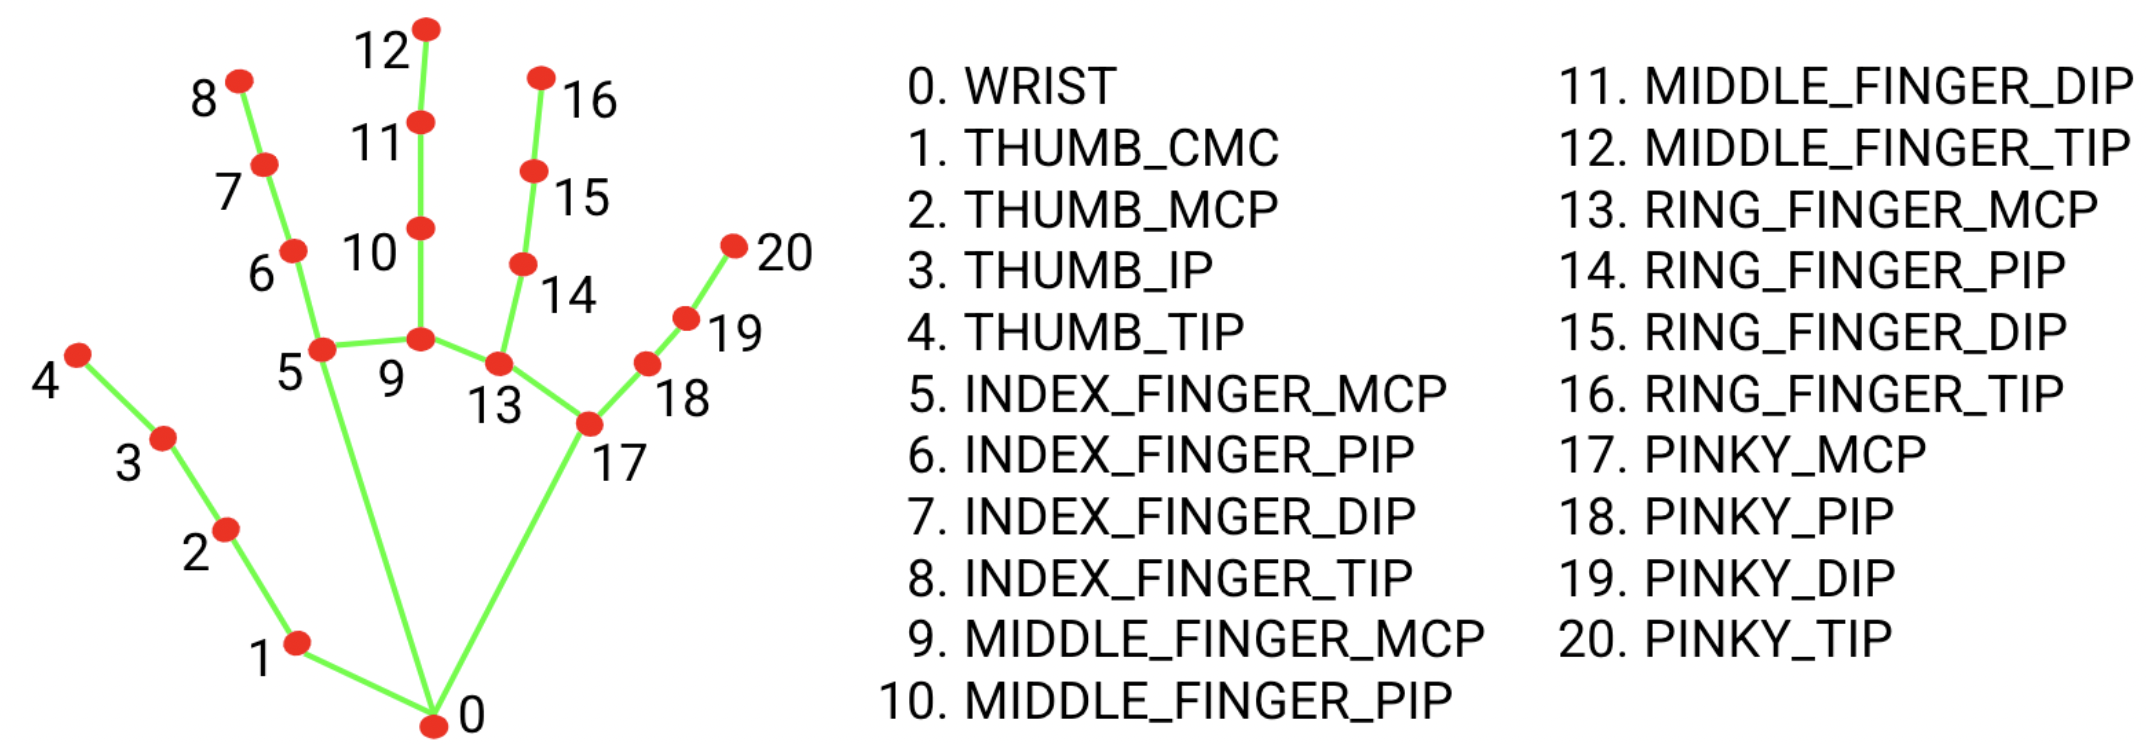
\includegraphics[width=0.9\linewidth]{content/images/mediapipe_landmarks.png}
    \caption{Hand-Landmarken-Modell nach Google MediaPipe \parencite{imageMediapipe_hand_landmarker}}
    \label{fig:mediapipe}
\end{figure}

Ein zentraler Schritt besteht anschließend in der Überführung der Trackingdaten in eine zweidimensionale Cursorposition. Hierfür wird die Handposition auf den Bildschirmraum abgebildet. Der resultierende Cursor dient als primäres Eingabeelement für die Menüinteraktion. Dadurch entsteht eine direkte Kopplung zwischen Handbewegung im Kamerabild und Navigation innerhalb des Intreaktionssystems.
Neben der Positionsbestimmung erfolgt auch die Erkennung diskreter Gesten, wie in Abschnitt~\ref{sec:synthese_konzeption_des_interaktionssystems} erwähnt. Verwendet werden eine offene Hand zur Aktivierung der Menüinteraktion, eine Grab-Geste zur schnellen Bestätigung, sowie eine Pinch-Geste zur kontinuierlichen Steuerung von Slidern. Die Gestenerkennung basiert auf Distanzmaßen zwischen ausgewählten Landmarken (visualisiert in Abbildung \ref{fig:gesture_images_photos}), beispielsweise zwischen Fingerspitzen und Handbasis oder zwischen Daumen und Zeigefinger. Diese Heuristiken ermög\-lichen eine einfache, nachvollziehbare und in Echtzeit ausführbare Klassifikation.  Die erkannten Gesten dienen anschließend als Eingaben für eine zustandsbasierte Interaktionslogik, welche das Verhalten des Menüs steuert.
%Bei der Geste zur Aktivierung wurde zusätzlich darauf geachtet, dass die Geste nur bei frontaler Erkennung ausgelöst wird, um sicherzustellen, dass nur die Kamera an der aktuell frontalen Projektionsfläche das Menü aktivieren kann.

\begin{figure}[H]
\centering
\begin{subfigure}[t]{0.32\textwidth}
    \centering
    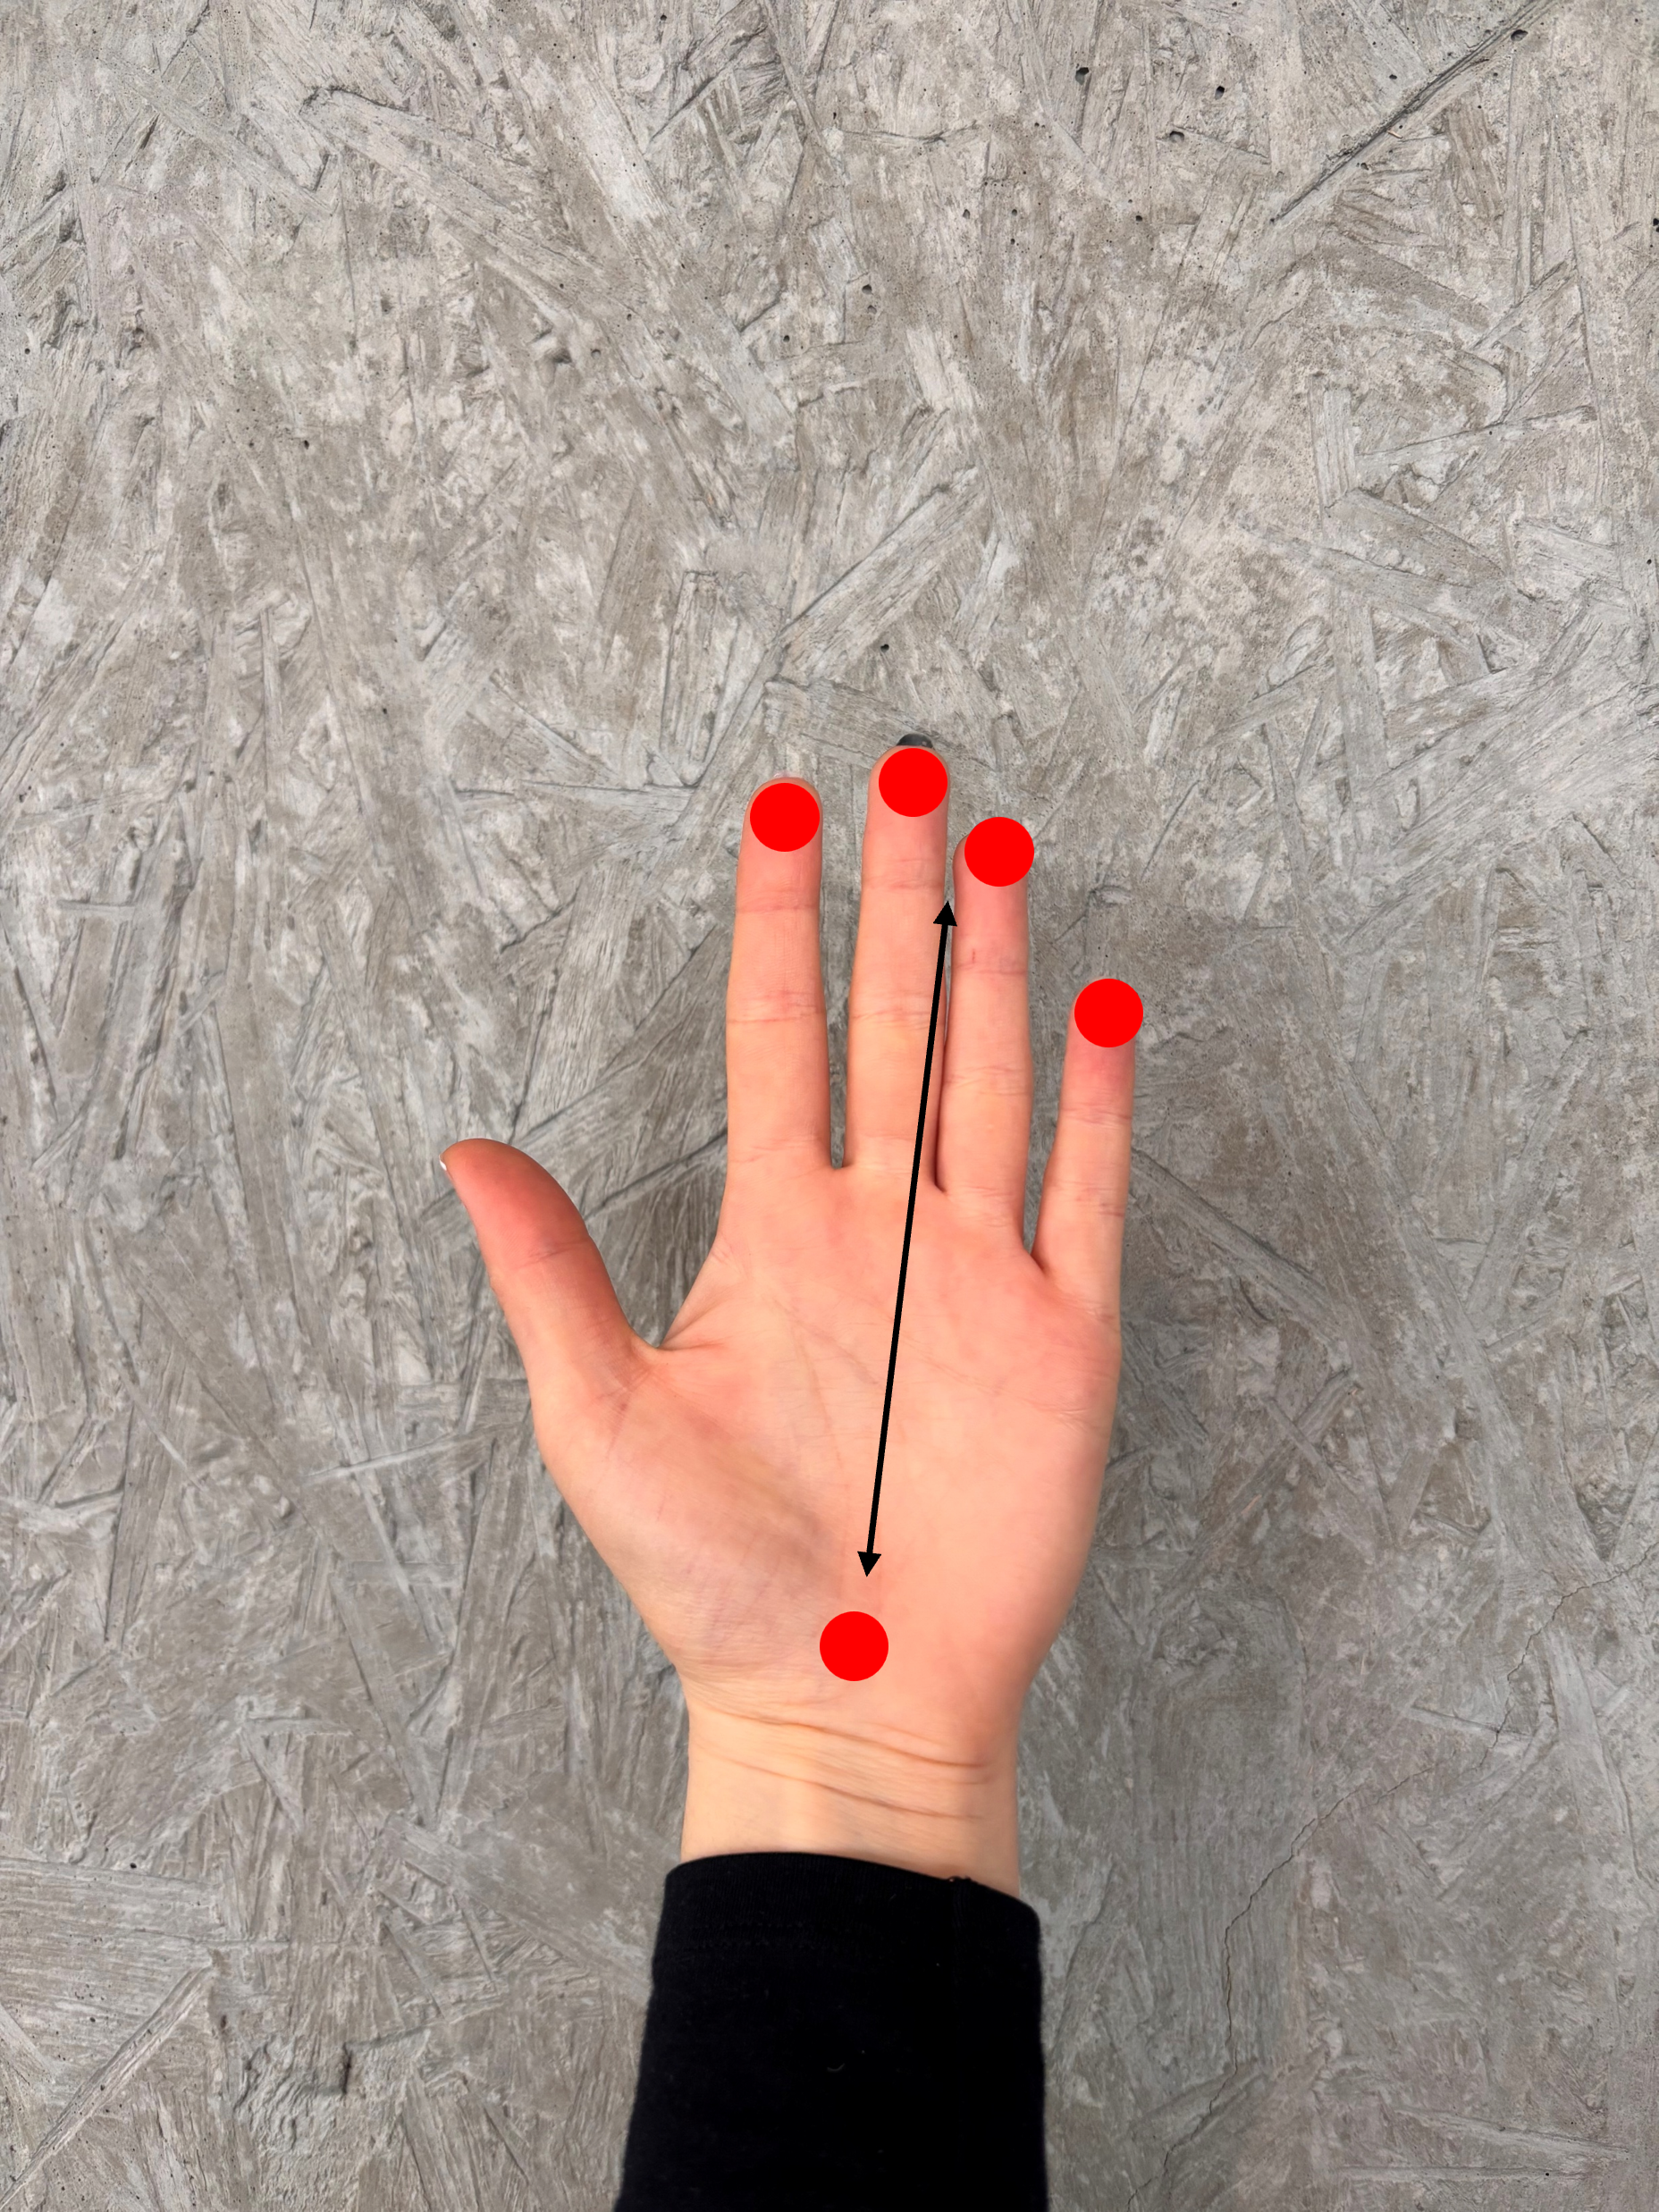
\includegraphics[width=\linewidth]
    {content/images/open_palm_gesture_image.png}
    \caption{Open-Palm-Geste nutzt den Abstand von allen Finger\-spitzen (außer Daumen) und der Handballenunterseite, sowie Spitze von Daumen und kleinem Finger}
    \label{fig:openpalm_gesture_image}
\end{subfigure}
\hfill
\begin{subfigure}[t]{0.32\textwidth}
    \centering
    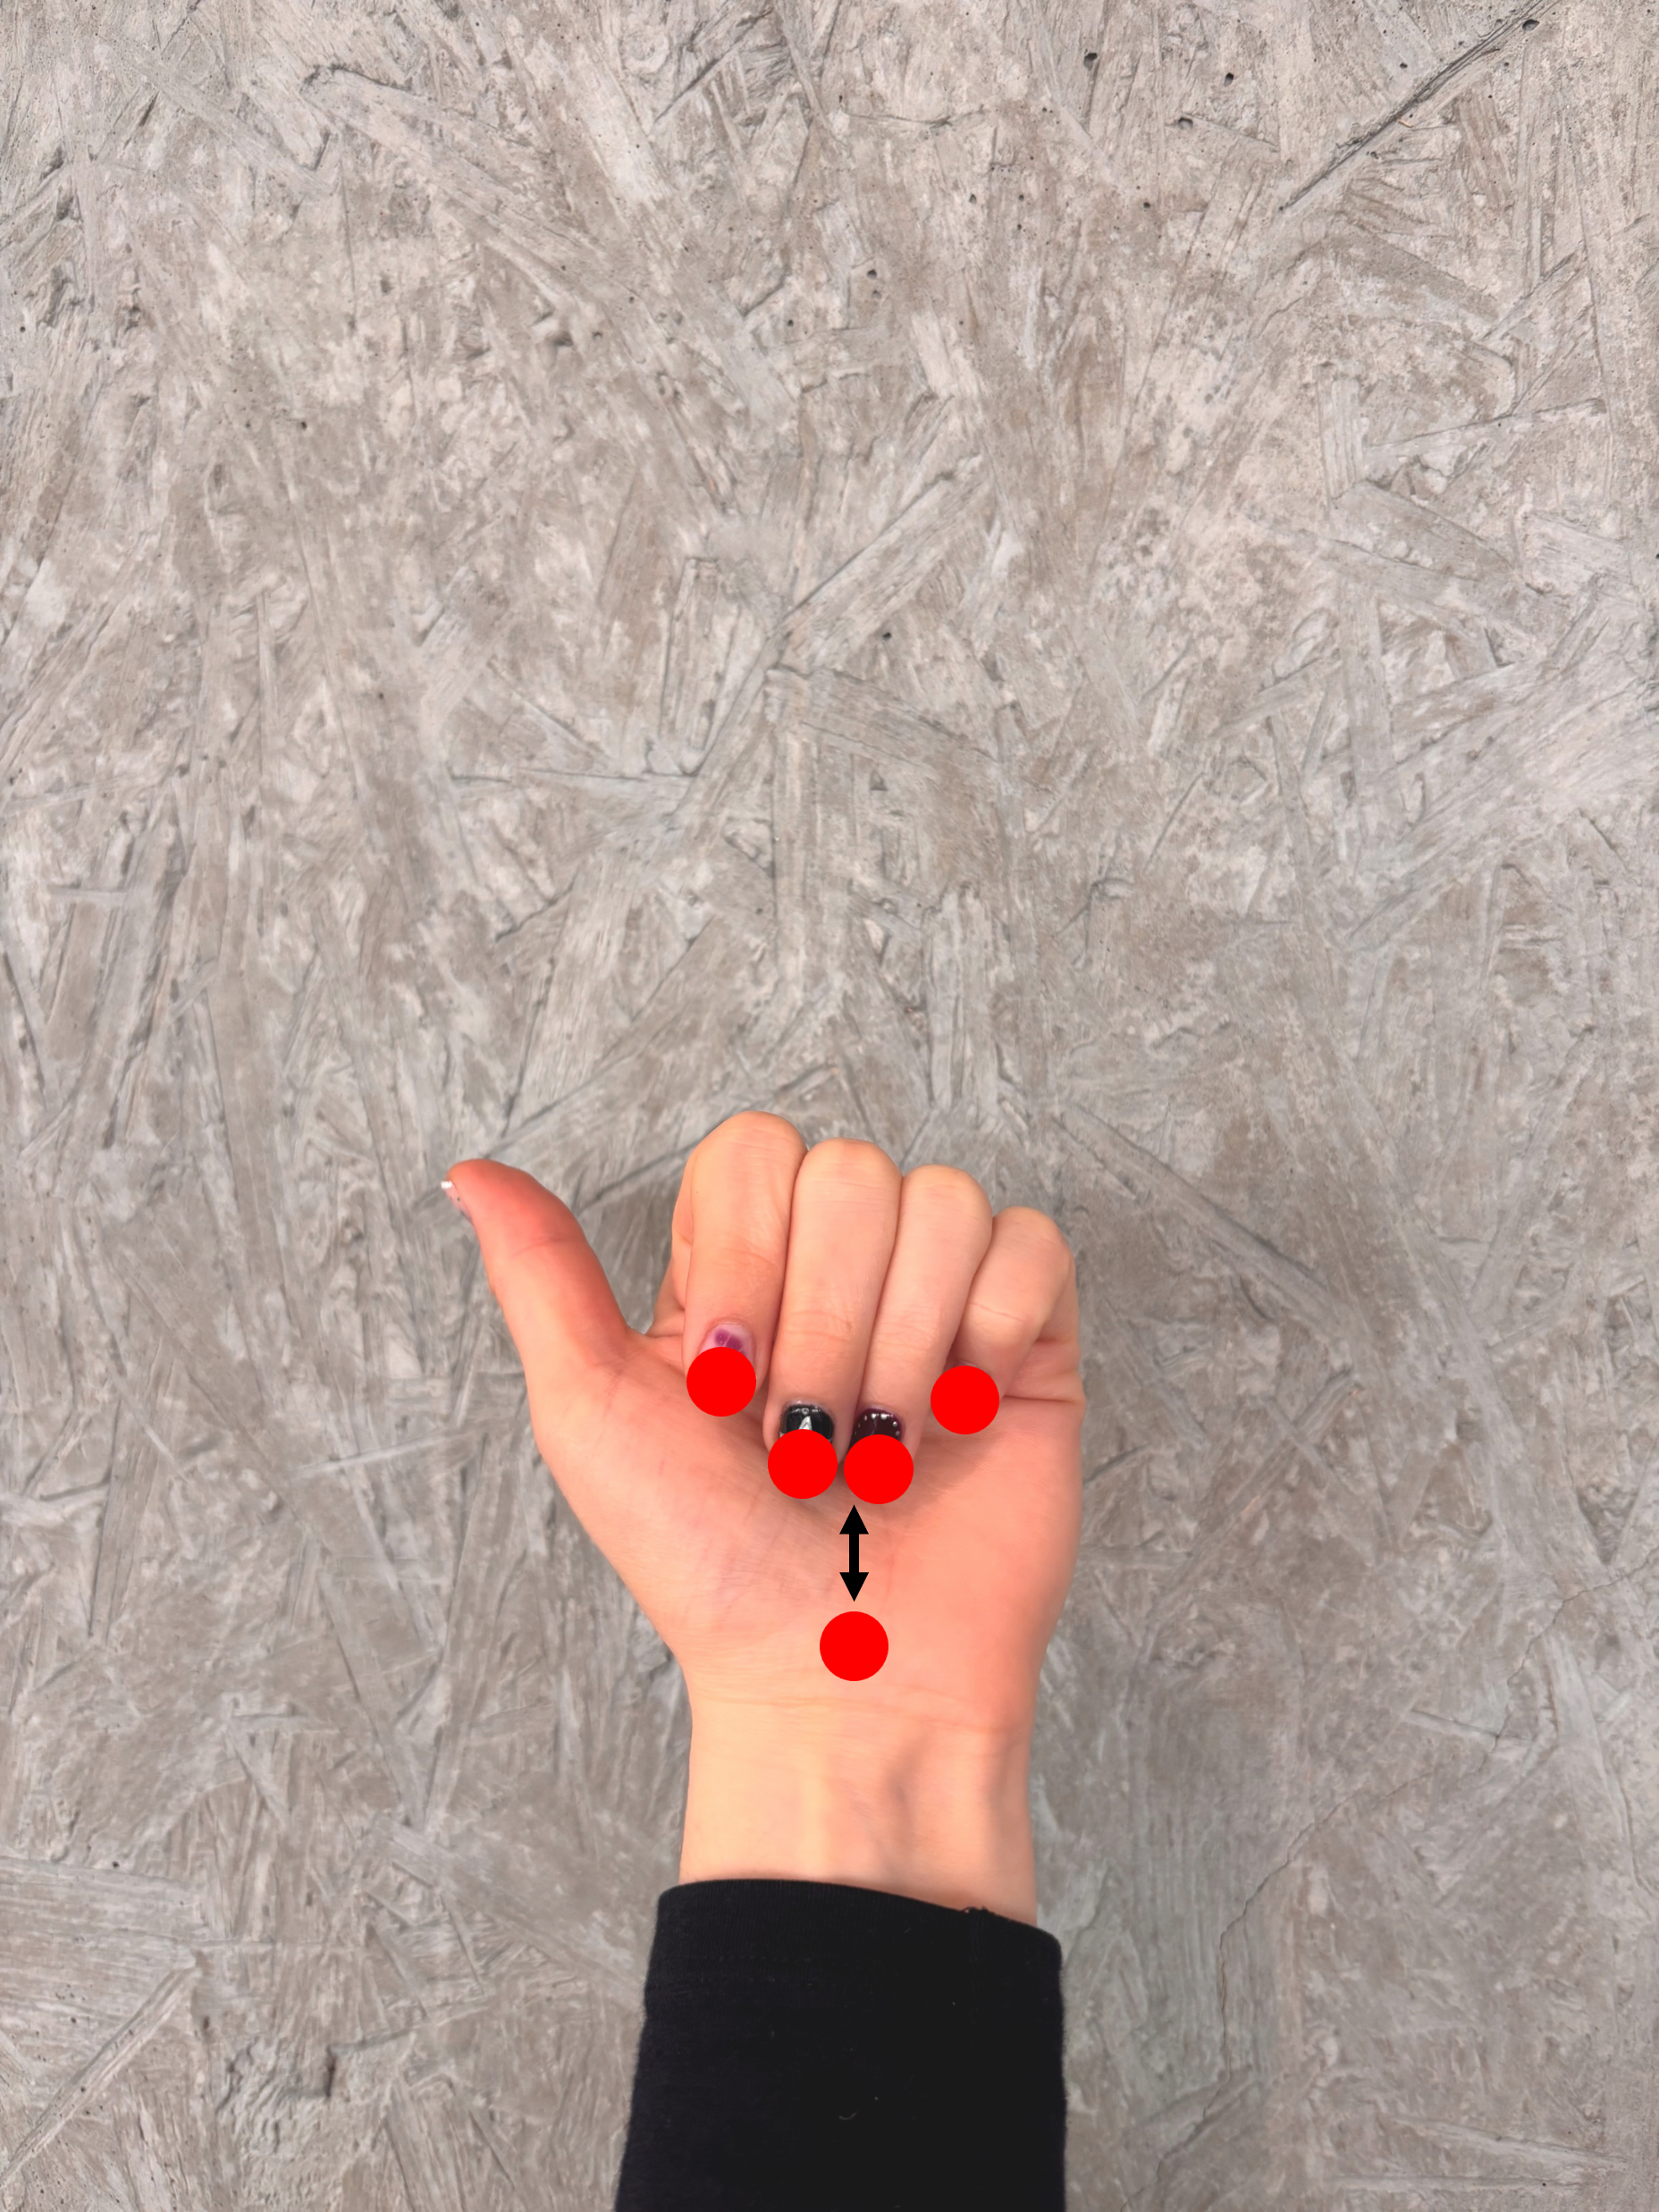
\includegraphics[width=\linewidth]
    {content/images/grab_gesture_image.png}
    \caption{Grab-Geste nutzt den Abstand zwischen allen Fingerspitzen (außer Daumen) und der Handballenunterseite}
    \label{fig:grab_gestute_image}
\end{subfigure}
\hfill
\begin{subfigure}[t]{0.32\textwidth}
    \centering
    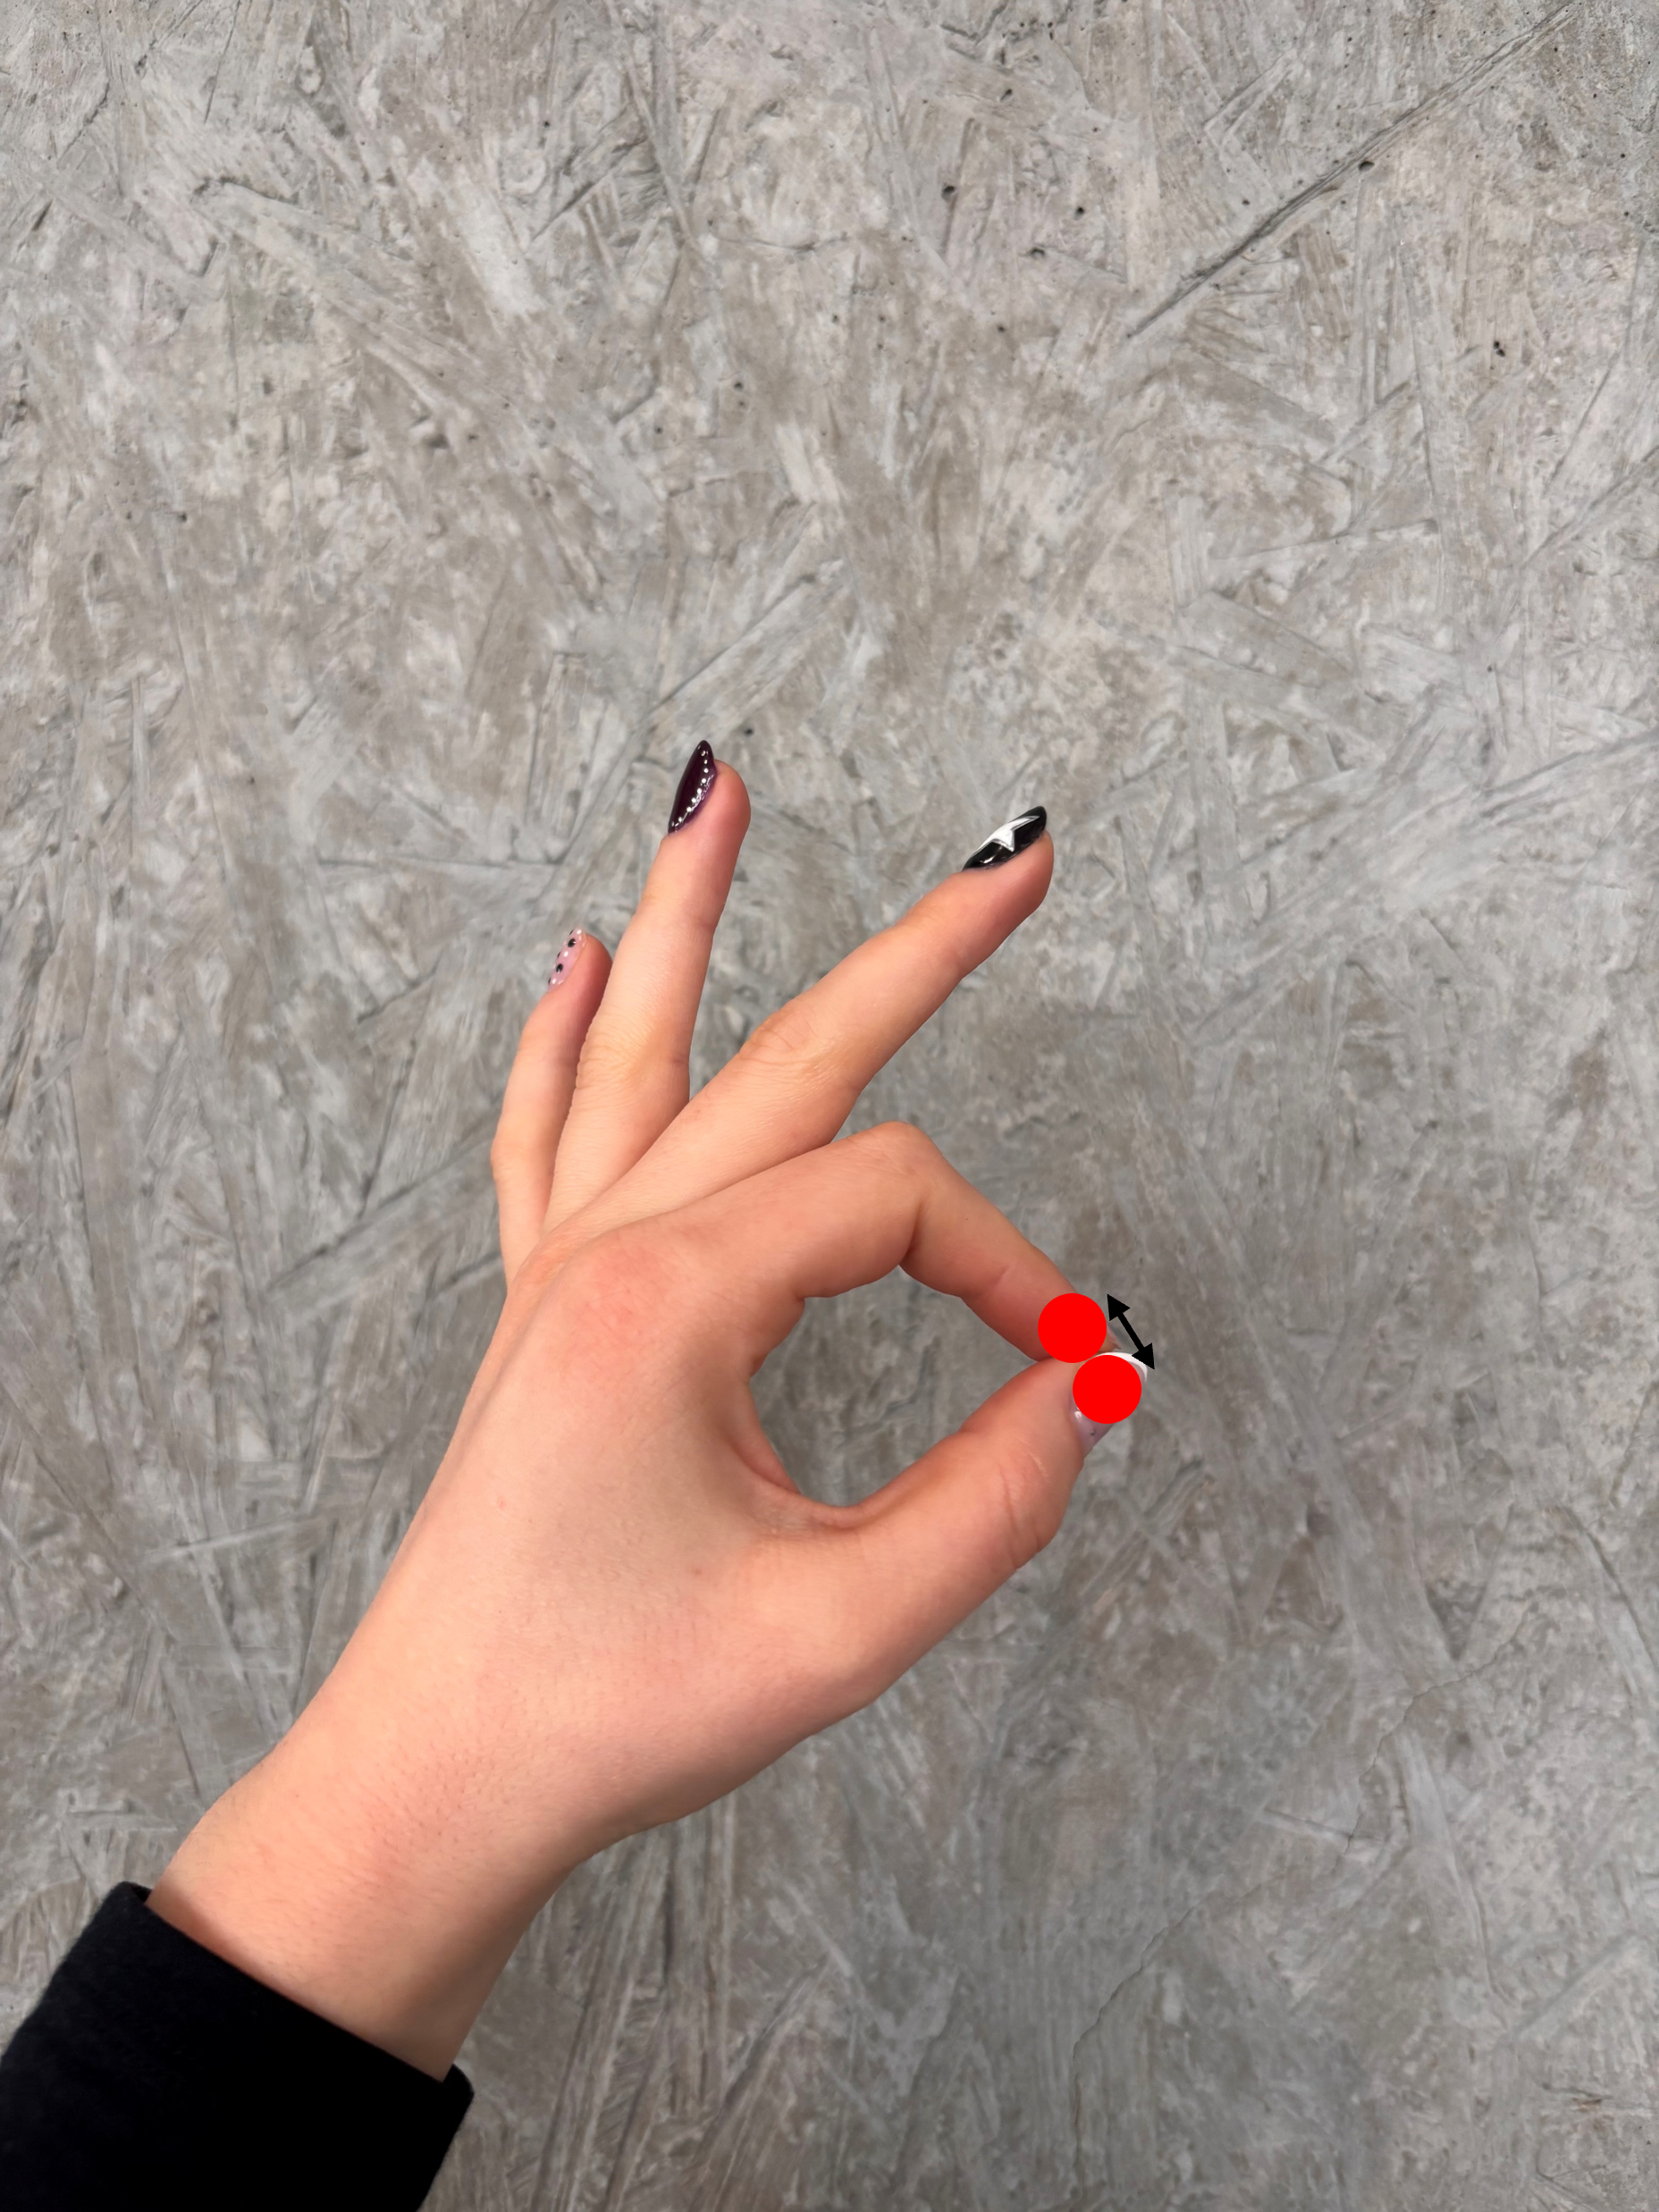
\includegraphics[width=\linewidth]
    {content/images/pinch_gesture_image.png}
    \caption{Pinch-Geste nutzt den Abstand zwischen der Zeigefingerspitze und Daumenspitze}
    \label{fig:pinch_gesture_image}
\end{subfigure}
\caption{Verwendete Gesten und die jeweils zur heuristischen Erkennung herangezogenen Landmarken bzw. Distanzbeziehungen (dargestellt in rot).}
\label{fig:gesture_images_photos}
\end{figure}

Die Handtracking-Pipeline ist eng mit einer Zustandslogik gekoppelt, die den Ablauf der Interaktion steuert (siehe Abbildung~\ref{fig:state_flow_diagram_alt}). Dabei lassen sich mehrere Zustände unterscheiden, die abhängig von der Handerkennung und dem Interaktionsverhalten der Nutzer:innen durchlaufen werden.
Im Ausgangszustand \textit{Activation} ist kein Menü sichtbar. Wird eine Hand erkannt, kann durch Ausführen der Aktivierungsgeste ein Übergang in den Aktivierungsprozess initiiert werden. Wird diese Geste über eine Dauer von drei Sekunden stabil erkannt, wird sie bestätigt und das Menü eingeblendet. Dadurch wird verhindert, dass zufällige oder kurzzeitige Erkennungen unmittelbar zu einer Interaktion führen.
Nach erfolgreicher Aktivierung wechselt das System in den Zustand \textit{Menu}, in dem das Menü sichtbar ist und aktiv genutzt werden kann. Solange eine Hand erkannt wird, bleibt dieser Zustand bestehen und ermöglicht die Interaktion mit den Menüelementen.
Wird keine Hand mehr erkannt, wechselt das System in den Zustand \textit{Idle}, in dem das Menü weiterhin sichtbar bleibt, jedoch keine aktive Interaktion erfolgt. Wird innerhalb dieses Zustands erneut eine Hand erkannt, kehrt das System in den Menüzustand zurück.
Bleibt die Handerkennung für einen längeren Zeitraum aus (mehr als drei Sekunden), wird ein Dwell-Mechanismus ausgelöst, der in den Zustand \textit{Dwell} führt. In diesem Zustand verblasst das Menü visuell, während ein Timer abläuft. Wird innerhalb dieser Phase keine neue Interaktion initiiert, kehrt das System schließlich in den Ausgangszustand \textit{Activation} zurück, in dem das Menü nicht mehr sichtbar ist.
Der Fortschritt der Aktivierung sowie der Übergang in den Dwell-Zustand werden jeweils durch visuelles Feedback im Overlay des Inter\-aktions\-systems vermittelt, sodass Nutzer:innen den aktuellen Interaktionsstatus jederzeit nachvollziehen können.

\begin{figure}[H]
    \centering
    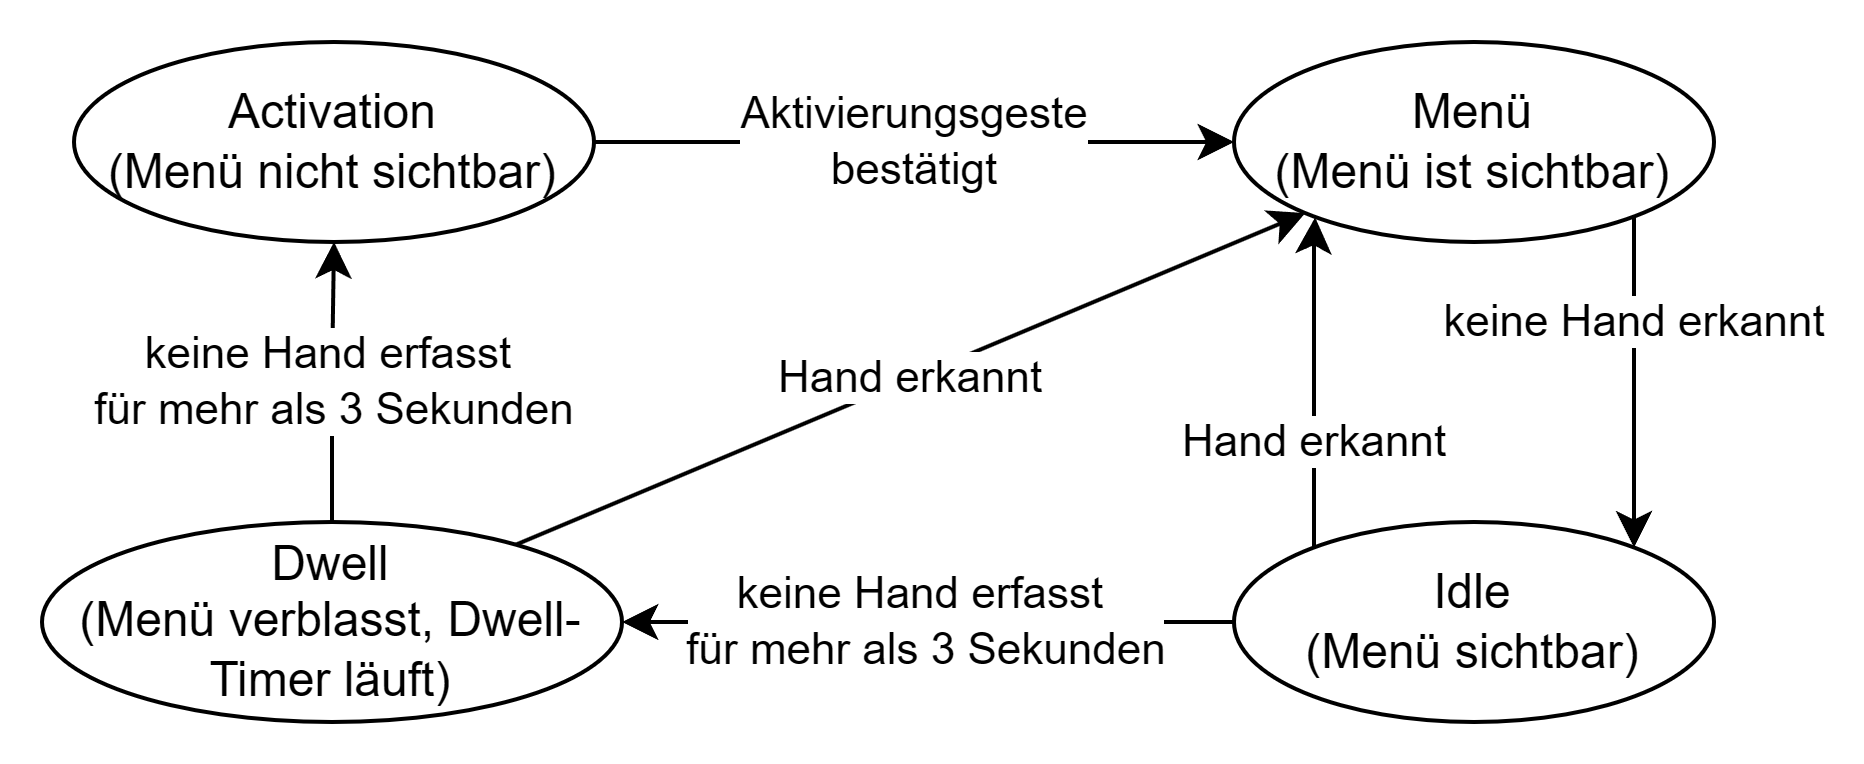
\includegraphics[width=0.8\linewidth]{content/diagrams/state_flow_diagram_alt}
    \caption{Visuali\-sierung der Interaktions\-zustände.}
    \label{fig:state_flow_diagram_alt}
\end{figure}


\subsection{Electron-Overlay}

Die Umsetzung des Interaktionssystems (im als Folgenden \textit{Overlay} bezeichnet, was das gesamte Interaktionssystem einschließlich Benutzungsoverfläche, Interaktionslogik und Kommunikationsschnittstelle umfasst) erfolgt in Form einer modular aufgebauten Electron-Anwendung.
Die Projektstruktur ist so gestaltet, dass Interaktionslogik, Benutzungsoberfläche und Systemintegration klar voneinander getrennt sind.
Listing~\ref{lst:project_structure} zeigt die grundlegende Ordner- und Dateistruktur der Anwendung.
\begin{lstlisting}[
    caption={Projektstruktur der Electron-Anwendung},
    label={lst:project_structure},
    basicstyle=\ttfamily\small
]
gesture-interface/
|-- electron-app/           # Electron-Anwendung
|-- images/                 # UI-Grafiken und Assets
|-- js/                     # Zentrale Interaktionslogik
|   |-- cameraSelector.js   # Kamerakalibrierung
|   |-- cursor.js           # Cursorberechnung
|   |-- data.js             # Datenmodell
|   |-- debugControls.js    # Debugfunktionen
|   |-- gestures.js         # Gestenerkennung
|   |-- main.js             # Einstiegspunkt
|   |-- menu.js             # Menuelogik
|   |-- slider.js           # Slidersteuerung
|   |-- timings.js          # Zustands-Timing
|   `-- websocket.js        # Kommunikation
|-- lib/                    # Externe Bibliotheken (MediaPipe)
|-- index.html              # UI-Struktur
|-- offlineMenu.json        # Menuedefinition
`-- style.css               # Styling
\end{lstlisting}

Die Struktur verdeutlicht die Trennung zwischen der Interaktionslogik im Verzeichnis \texttt{js/},
der visuellen Darstellung über HTML und CSS sowie der Systemintegration durch Electron.
Insbesondere sind Gestenerkennung, Menülogik und Zustandsverwaltung als eigenständige Module implementiert,
was eine klare Strukturierung der Anwendung sowie eine erleichterte Erweiterbarkeit ermöglicht.
Aufbauend auf dieser modularen Struktur wird im Folgenden die technische Umsetzung des Overlays näher erläutert.


\subsubsection{Technische Umsetzung}
\label{sec:technische_umsetzung}
Das visuelle Interaktionssystem wurde als Overlay mit \textit{Electron} umgesetzt.
Electron ist eine Open-Source-Plattform zur Entwicklung plattformübergreifender Desktopanwendungen auf Basis von Webtechnologien \parencite{electronDocumentation}. Anwendungen werden dabei in einer Chromium-Umgebung ausgeführt, also innerhalb einer auf dem Open-Source-Webbrowser Chromium basierenden Laufzeitumgebung, und können gleichzeitig auf systemnahe Funktionen zugreifen.
Die Wahl von Electron ermöglicht eine flexible und plattformunabhängige Implementierung der Benutzungsoberfläche, wodurch das Overlay unabhängig von der jeweiligen Zielanwendung ausgeführt werden kann.
Electron wird dabei als eigenständiger UI-Layer genutzt, der unabhängig von der jeweils gesteuerten Anwendung arbeitet. Diese Trennung ist wesentlich, da das Menü nicht als Bestandteil einer konkreten Zielanwendung implementiert werden soll.
Durch diese Architektur kann das Interaktionssystem als zusätzliche Steuerungsschicht über bestehende Anwendungen gelegt werden, ohne dass diese selbst angepasst werden müssen.


\subsubsection{Visuelle Darstellung und Rückmeldungen}
Das Interaktionssystem wird als transparentes Overlay über der eigentlichen Anwendung dargestellt. Innerhalb dieses Overlays werden sämtliche visuellen Elemente der Interaktion gerendert, ohne die Darstellung der zugrunde liegenden Anwendung zu verdecken. Dabei ist das Fenster standardmäßig nicht fokussierbar, sodass Tastatureingaben weiterhin an die darunterliegende Anwendung weitergeleitet werden können. Dies ist insbesondere relevant, da die Zielanwendung in vielen Szenarien parallel über klassische Eingabegeräte steuerbar bleiben soll.

Innerhalb des Overlays werden das Marking-Menu, der Cursor, visuelle Statusanzeigen sowie kontextabhängige Steuerelemente wie Slider dargestellt. Die Darstellung folgt den in Abschnitt~\ref{sec:synthese_visual_feedback} beschriebenen Gestaltungsentscheidungen und setzt diese technisch innerhalb eines Canvas-Elements um.
Da die Handtracking-Pipeline kontinuierlich pro Frame aktualisierte Positions- und Gestendaten liefert, basiert die Darstellung auf einem framebasierten Renderansatz. Das Menü sowie der Cursor werden bei jeder Aktualisierung vollständig neu gezeichnet, sodass zu jedem Zeitpunkt ausschließlich der aktuelle Interaktionszustand sichtbar ist. Dieses Vorgehen ermöglicht eine konsistente und latenzarme Darstellung dynamischer Zustandsänderungen und vereinfacht die Synchronisation zwischen Trackingdaten, Interaktionslogik und visueller Ausgabe.

Für die konkrete Interaktion ist entscheidend, wie die aktuelle Cursorposition einem Menüelement zugeordnet wird. Die Bestimmung des fokussierten Menüelements basiert auf der relativen Position des Cursors zum Zentrum des Menüs. Hierfür wird die Cursorposition in Polarkoordinaten überführt, wobei insbesondere der Winkel und der Abstand zum Menüzentrum berücksichtigt werden. Der Winkel bestimmt, in welches Segment des radialen Menüs der Cursor fällt, während der Abstand verwendet wird, um zwischen den Menüebenen zu unterscheiden. Auf diese Weise kann eindeutig bestimmt werden, welches Menüelement aktuell fokussiert ist. Dieses Verfahren ermöglicht eine kontinuierliche und stabile Zuordnung von Cursorbewegungen zu Menüsegmenten und bildet die Grundlage für die Steuerung des Marking-Menus.

Das Marking-Menu ist datengetrieben implementiert. Die Menüstruktur wird nicht fest in der Oberfläche hinterlegt, sondern zur Laufzeit aus einer externen JSON-Konfiguration geladen, die von der Zielanwendung bereitgestellt wird. Dadurch können Anzahl der Einträge, Hierarchie und zugehörige Aktionen dynamisch angepasst werden, ohne Änderungen an der Benutzeroberfläche vornehmen zu müssen. Der inhaltliche Aufbau sowie die Gestaltung der Interaktionszustände wurden bereits in Abschnitt~\ref{sec:synthese_konzeption_des_interaktionssystems} beschrieben.

Für Entwicklungs- und Konfigurationszwecke kann das Overlay temporär in einen Konfigurationsmodus versetzt werden. In diesem Modus werden Tastatur- und Mauseingaben abgefangen und für Kalibrierungsfunktionen genutzt. Der Konfigurationsmodus wird in Abschnitt~\ref{sec:development} näher erläutert.


\subsubsection{Zustandslogik der Menüinteraktion}
Die Interaktionslogik des Menüs fußt auf einer zustandsbasierten Struktur, die die aktuelle Interaktion der Nutzer:innen mit den Menüelementen abbildet.
Für jede aktive Menüebene (Level) wird ein separater Interaktionszustand verwaltet.
Ein solcher Zustand umfasst Informationen über das aktuell vom Cursor fokussierte Element, das bereits ausgewählte Element sowie den Fortschritt eines Dwell-Timers zur automatischen Auswahl.
Zusätzlich werden Zustandsinformationen wie das zuvor fokussierte Element oder der Status einer aktiven Greifgeste gespeichert.
Die Verwaltung von Interaktions\-zuständen je Level ermöglicht eine konsistente Verarbeitung mehrstufiger Menühierarchien. Eine Visuali\-sierung der Level ist in Abbildung \ref{fig:levels} dargestellt.

\begin{figure}[H]
    \centering
    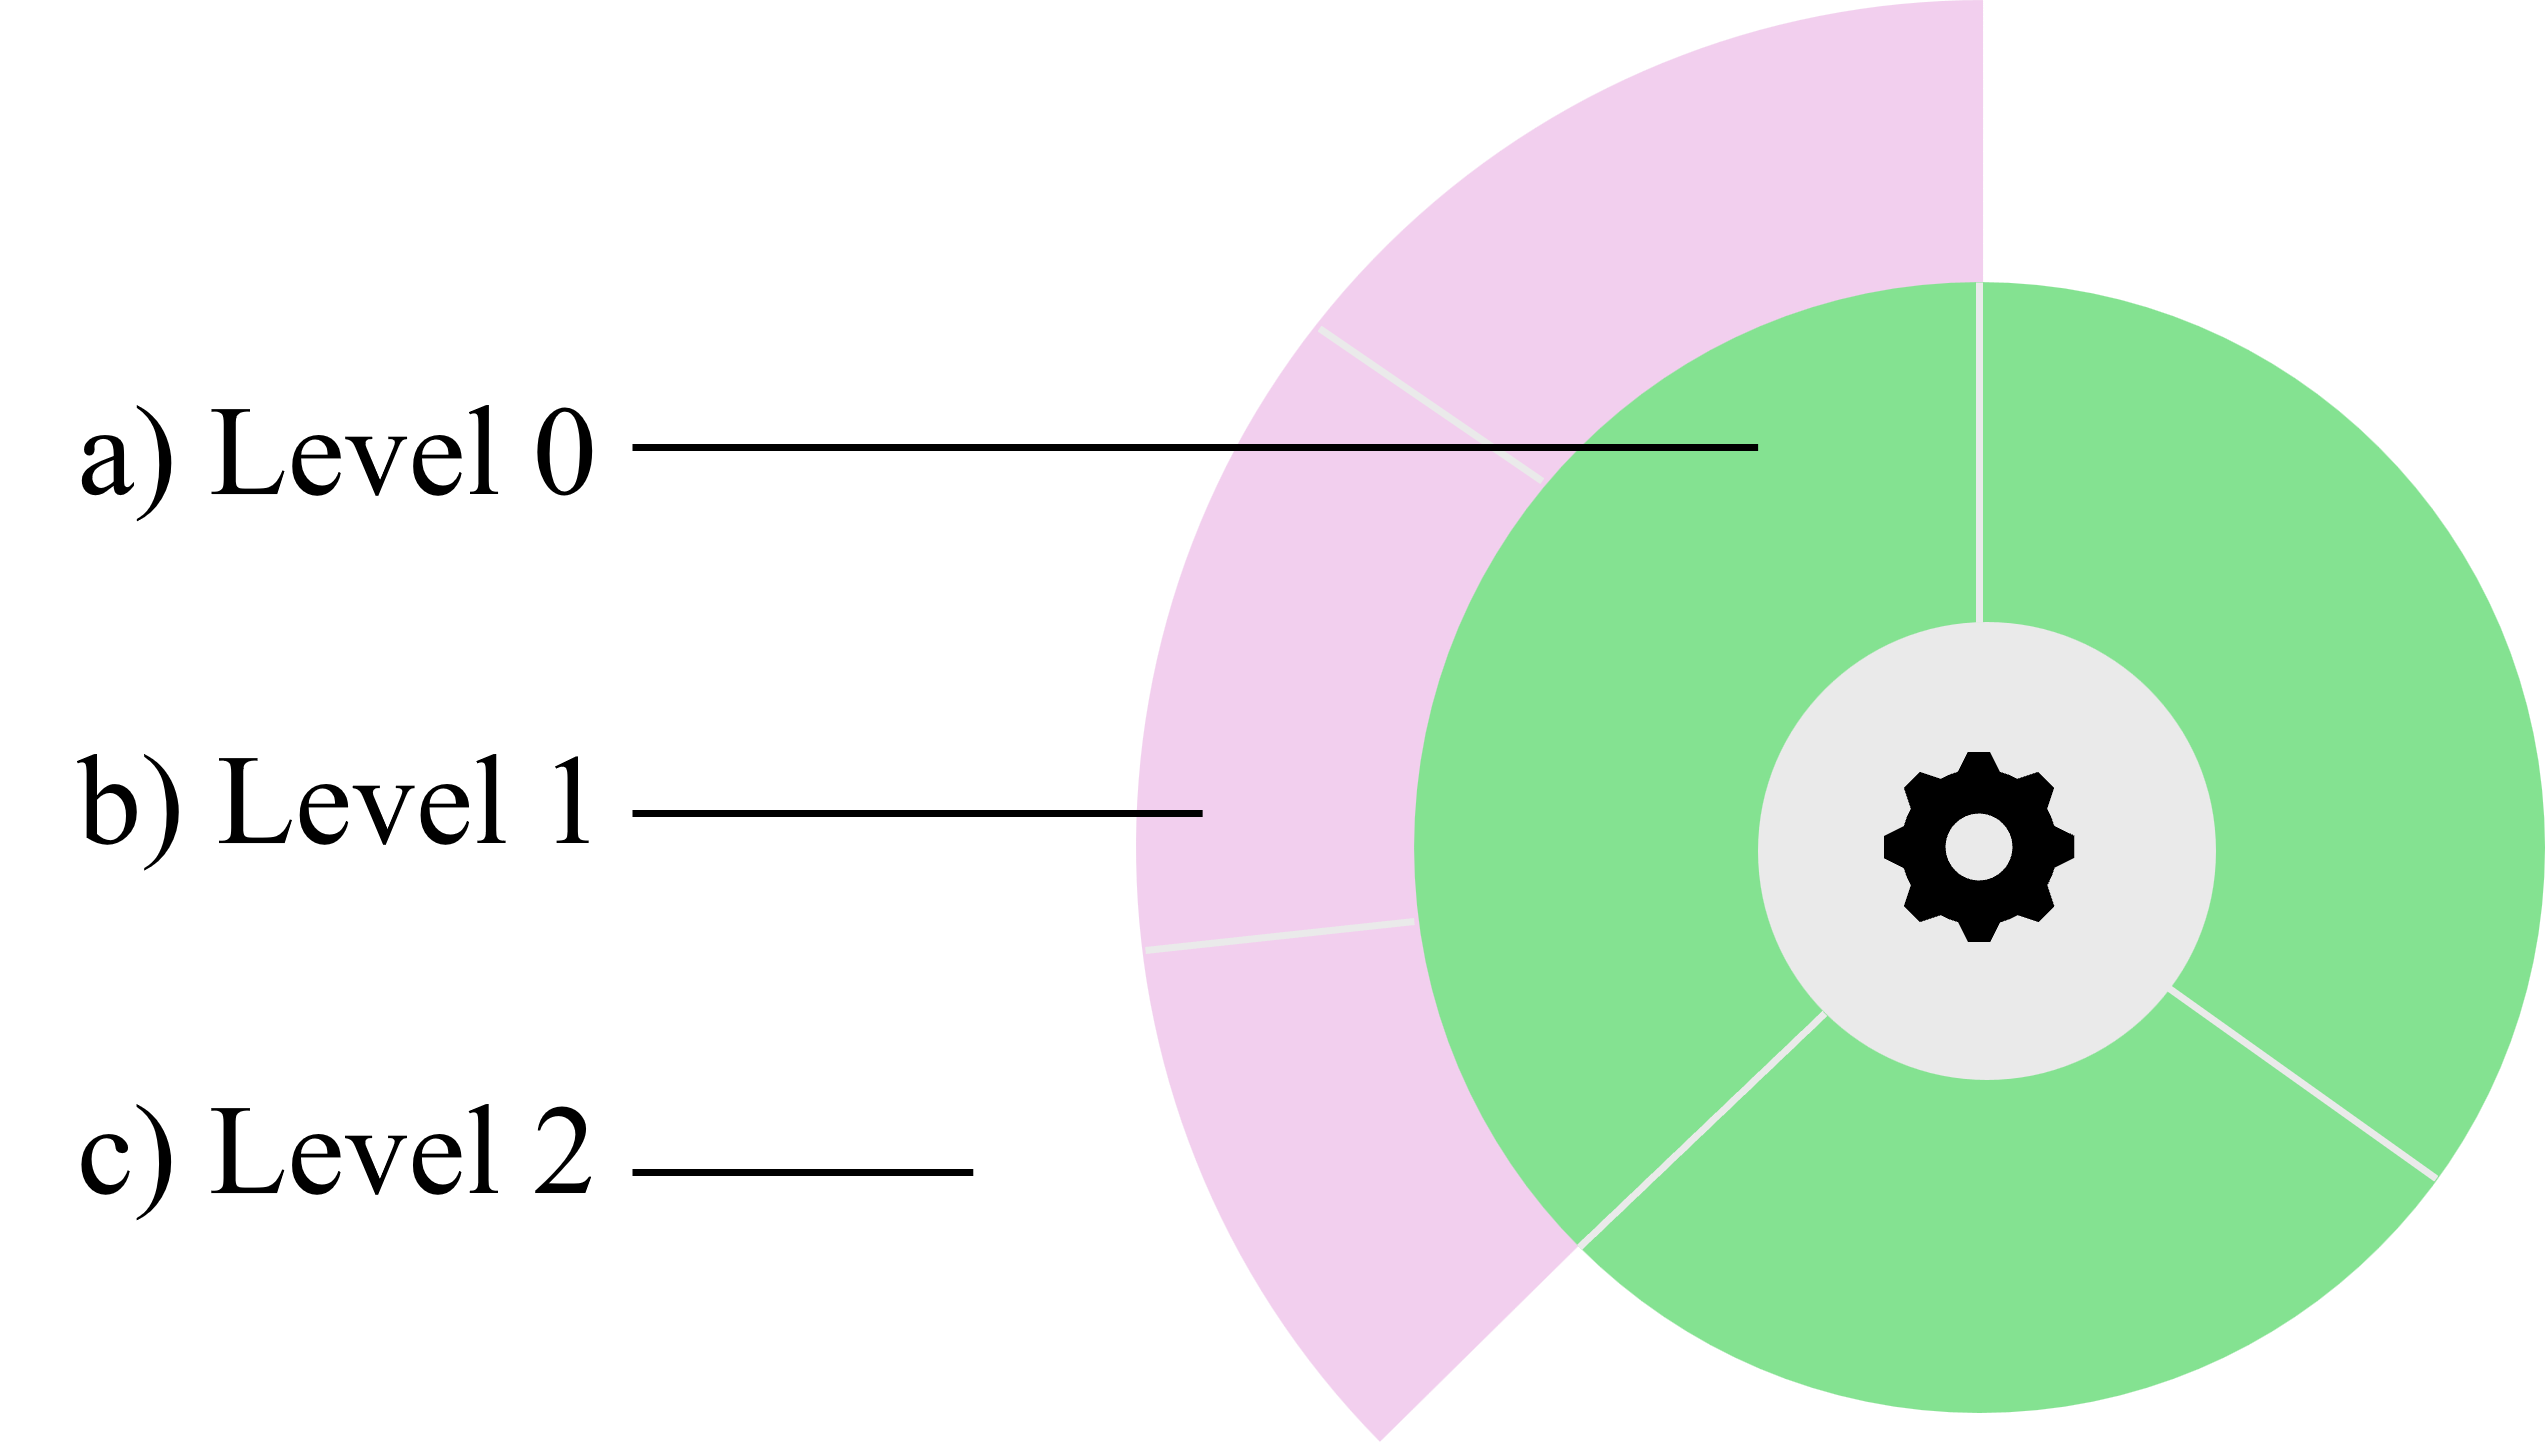
\includegraphics[width=0.45\linewidth]{content/images/levels.png}
    \caption{Visuali\-sierung der Menüebenen (Level) im Menü.}
    \label{fig:levels}
\end{figure}

Für jede Ebene können dadurch unabhängige Hover-, Auswahl- und Dwell-Zustände geführt werden. 
Gleichzeitig unterstützt diese Struktur eine iterative Verarbeitung während des Renderings, da alle aktiven Ebenen sequenziell ausgewertet werden können.


Zur Erkennung von Zustandsänderungen zwischen einzelnen Frames werden zusätzlich vorherige Interaktions\-zustände gespeichert.
Dadurch werden Änderungen wie ein Wechsel des fokussierten Menüelements oder das erstmalige Auftreten einer Greifgeste zuverlässig erkannt.
Diese framebasierte Zustandsverfolgung trägt zu einer möglichst stabilen und konsistenten Interaktionsauswertung bei.

Listing~\ref{lst:levelstates} zeigt beispielhaft eine Funktion zur Erzeugung eines Interaktionszustands für eine einzelne Menüebene. 
Die Funktion gibt ein Zustandsobjekt mit den relevanten Interaktionsparametern zurück und kann entsprechend der Anzahl aktiver Menüebenen mehrfach instanziiert werden.

Die Trennung zwischen globalem Systemzustand (siehe Abschnitt~\ref{sec:handtracking-pipeline}), UI-Zustand und Interaktionszustand verbessert die Erweiterbarkeit des Systems und reduziert Kopplungen zwischen Tracking, Darstellung und Interaktionslogik.
Diese Zustandsstruktur bildet die Grundlage für die Auswertung der Nutzerinteraktionen sowie für die Darstellung der visuellen Rückmeldungen im Menü.

\begin{lstlisting}[language=JavaScript,caption={Beispielhafte Struktur eines Interaktionszustands pro Menüebene},label={lst:levelstates},basicstyle=\ttfamily\footnotesize]
function createLevelState() {
    return {
        // Menuelement, das gerade gehovert wird
        hover: null,
        // Menuelement, das gerade ausgewaehlt ist
        selected: null,
        // Zeitpunkt, zu dem Dwell gestartet ist
        dwellStart: null,
        // Fortschritt des Dwells in Prozent
        dwellProgress: 0,
        // Gibt an, ob dwell bereits getriggert wurde
        dwellTriggered: false,
        // Menuelement, das im letzten Frame gehovert wurde
        previousHover: null,
        // Gibt an, ob Grab-Geste im letzten Frame ausgeloest war
        wasGrabbing: false
    };
}
\end{lstlisting}


\subsection{Datengetriebene Menüstruktur}
Da das im Overlay dargestellte radiale Menü nicht statisch implementiert ist, sondern von der Zielanwendung konfiguriert wird, muss es eine definierte Struktur geben, wie das Menü aufgebaut sein darf. Die Struktur des Menüs wird durch eine JSON-basierte Konfiguration beschrieben, die von der Zielanwendung an das Overlay übermittelt wird. Dadurch kann die Menüstruktur dynamisch angepasst werden, ohne Änderungen an der Benutzungsoberfläche selbst vornehmen zu müssen. Das Overlay ist damit ausschließlich für Darstellung und Interaktionslogik verantwortlich.

Die Konfiguration des Menüs definiert sowohl globale Eigenschaften des Menüs, wie beispielsweise den Radius der Hauptmenüebene oder die Größe von Untermenüs, als auch die einzelnen Menüeinträge.
Ein Menüeintrag kann dabei entweder als Navigationsknoten fungieren, der ein weiteres Untermenü öffnet, oder direkt eine Interaktion auslösen, etwa die Aktivierung eines Buttons oder die Steuerung eines kontinuierlichen Parameters über einen Slider. Dadurch entsteht eine klare Trennung zwischen Navigations- und Aktionsknoten.

Die hierarchische Organisation ermöglicht es, mehrere Interaktionsfunktionen innerhalb einer begrenzten Anzahl sichtbarer Menüsegmente bereitzustellen. 
Während die oberste Ebene zentrale Funktionskategorien enthält, werden detailliertere Steuerungsoptionen innerhalb der entsprechenden Untermenüs zugänglich gemacht.
Jeder Menüeintrag besitzt eine eindeutige Identifikationsnummer (``\texttt{id}'') sowie Metadaten wie eine Bezeichnung (``\texttt{label}''), ein Icon (``\texttt{icon}'') und den Typ des UI-Elements (``\texttt{type}''). Der Typ bestimmt, wie ein Eintrag im Interaktionssystem interpretiert wird, beispielsweise als Untermenü (``\texttt{menu}''), als kontinuierliches Steuerelement (``\texttt{slider}'') oder als diskrete Aktion (``\texttt{button}'').

Abhängig vom Typ des Eintrags können zusätzliche Parameter definiert werden. Eine zentrale Rolle spielt dabei der Schlüssel ``\texttt{target}'', der angibt, welcher Parameter in der Zielanwendung durch die Interaktion beeinflusst wird. Im Fall eines Sliders wird beispielsweise ein kontinuierlicher Wert für den angegebenen Zielparameter übertragen, während bei einem Button diskrete Zustandsänderungen ausgelöst werden. Diese Informationen werden bei der Interaktion als Teil der WebSocket-Nachrichten an die Zielanwendung übermittelt (siehe Abschnitt~\ref{sec:eventcommunication}).

Listing~\ref{lst:menu_config} zeigt beispielhaft eine solche Menükonfiguration. Die oberste Ebene enthält zwei Haupteinträge: ``\texttt{Umgebungseinstellungen}'' und ``\texttt{Presentation}''. Beide Einträge sind vom Typ ``\texttt{menu}'' und enthalten jeweils weitere Untereinträge im Feld ``\texttt{children}''.
Der Eintrag ``\texttt{Umgebungs- einstellungen}'' definiert ein Untermenü mit drei Slidern zur Steuerung von ``\texttt{volume}'', ``\texttt{bright- ness}'' und ``\texttt{vibration}''. Diese entsprechen den globalen Systemparametern.
Der Eintrag ``\texttt{Presen- tation}'' enthält sowohl einen Slider (``\texttt{Timeline}'') zur Steuerung der Wiedergabeposition als auch einen Button (``\texttt{Play/Pause}'') zur Steuerung des Abspielzustands. Beide greifen auf denselben Zielparameter ``\texttt{presentation}'' zu, unterscheiden sich jedoch im Interaktionstyp.
Durch diese strukturierte Beschreibung entsteht zur Laufzeit ein hierarchisches radiales Menü, bei dem die oberste Ebene die beiden Kategorien darstellt und weitere Funktionen über Submenüs zugänglich gemacht werden. Die konkrete visuelle Ausprägung dieses Menüs entspricht den zuvor beschriebenen Menüstrukturen (siehe Abschnitt~\ref{sec:synthese_radiales_menü}).

Diese generische Beschreibung der Menüstruktur ermöglicht es dem Interaktionssystem, unabhängig von konkreten Anwendungsszenarien zu bleiben. Neue Funktionen oder zusätzliche Menü\-ebenen können ergänzt werden, ohne die Implementierung des Overlays selbst zu verändern. Auf diese Weise kann für jedes Anwendungsszenario eine spezifische Menüstruktur definiert werden.

\begin{lstlisting}[language=json,caption={Beispiel einer Menükonfiguration},
label={lst:menu_config},basicstyle=\ttfamily\footnotesize]
{
  "radius": 200,
  "subRadius": 100,
  "items": [
    {
      "id": 1,
      "label": "Umgebungseinstellungen",
      "type": "menu",
      "icon": "settings",
      "children": [
        {
          "id": 11,
          "label": "Volume",
          "type": "slider",
          "icon": "volume",
          "target": "volume"
        },
        {
          "id": 12,
          "label": "Brightness",
          "type": "slider",
          "icon": "brightness",
          "target": "brightness"
        },
        {
          "id": 13,
          "label": "Vibration",
          "type": "slider",
          "icon": "vibration",
          "target": "vibration"
        }
      ]
    },
    {
      "id": 2,
      "label": "Presentation",
      "type": "menu",
      "icon": "presentation",
      "children": [
        {
          "id": 21,
          "label": "Timeline",
          "type": "slider",
          "icon": "timeline",
          "target": "presentation"
        },
        {
          "id": 22,
          "label": "Play/Pause",
          "type": "button",
          "icon": "play",
          "target": "presentation"
        }
      ]
    }
  ]
}
\end{lstlisting}


\subsection{Eventkommunikation}
\label{sec:eventcommunication}
Die Interaktion mit dem Menü erzeugt Interaktionsereignisse, die an die angebundene Zielanwendung weitergeleitet werden. 
Hierfür wird eine WebSocket-basierte Kommunikation eingesetzt. Die Verwendung einer persistenten WebSocket-Verbindung vermeidet wiederholte Verbindungsaufbauten und reduziert damit Latenzzeiten bei der Übertragung von Interaktionsereignissen.

Über diese Verbindung werden sowohl Aktionen vom Overlay an die Zielanwendung gesendet als auch Initialwerte oder Bestätigungsnachrichten von der Anwendung an das Overlay zurückgegeben.
Damit entsteht eine kontinuierliche Kommunikationsschnittstelle zwischen Interaktionssystem und Anwendung.

\subsubsection{Nachrichtenstruktur}
Die übertragenen Nachrichten folgen einer einheitlichen JSON-Struktur (Tabelle \ref{tab:websocket_message}).
Dieses Schema ermöglicht die Beschreibung unterschiedlicher Interaktionsereignisse (zum Beispiel diskrete Buttonaktionen
oder kontinuierliche Slideränderungen) innerhalb eines einheitlichen Kommunikationsprotokolls.
Das Feld \texttt{action} (im Folgenden \textit{Aktion}) beschreibt das Interaktionsereignis.
Nachrichten mit der Aktion ``\texttt{update}'' werden bei Änderungen kontinuierlicher Werte verwendet, während ``\texttt{pressed}'' diskrete Button-Aktionen beschreibt. Nachrichten mit der Aktion ``\texttt{initial}'' werden für die Initialisierung genutzt und können initiale Sliderwerte oder die Menüstruktur selbst senden. Der Typ (``\texttt{type}'') einer Nachricht gibt an, welches Element die Nachricht ausgelöst hat. ``\texttt{slider}''-Typ Nachrichten gehören immer zur Aktion ``\texttt{update}'', während die ``\texttt{pressed}''-Aktion immer zum Typ ``\texttt{button}'' gehört und ``\texttt{type}'' ``\texttt{menu}'' immer zur Aktion ``\texttt{initial}''. Das ``\texttt{target}'' gibt immer das Ziel oder den Kontext der aktuellen Interaktion an, wie ``\texttt{volume}'' oder ``\texttt{presentation}''. \texttt{value} gibt an, welchen Wert die Aktion aktualisiert hat. Im Falle von Slidern sind das meist Angaben zwischen 0 und 1, für Buttons können es spezifische Klick-Events sein. Die ``\texttt{id}'' gibt an, zu welchem Menüelement die Aktion gehört, was nützlich ist, falls es beispielsweise mehrere Slider mit dem Ziel ``\texttt{volume}'' gibt.
Eine beispielhafte Nachricht ist in Listing \ref{lst:slider_update} dargestellt.

\begin{table}[h]
\centering
\begin{tabular}{lll}
\toprule
Feld & Beschreibung & Mögliche Werte \\
\midrule
action & Art der Interaktion & update, pressed, initial \\
type & Typ des UI-Elements & slider, button, menu \\
target & Zielparameter & volume, brightness, vibration, presentation \\
value & übertragener Wert & 0.0–1.0, play, pause \\
id & ID des Menüeintrags & 1, ... \\
\bottomrule
\end{tabular}
\caption{Übersicht über die Felder, die in einer Nachricht gesendet werden.}
\label{tab:websocket_message}
\end{table}


% Motivation für Wahl
Durch die Verwendung eines generischen Nachrichtenformats bleibt die Kopplung zwischen Interaktionssystem und Zielanwendung gering. Das Overlay übermittelt keine anwendungsspezifischen Methodenaufrufe, sondern abstrahierte Interaktionsereignisse. Dadurch kann das System prinzipiell mit unterschiedlichen Anwendungen kombiniert werden. Zusätzlich können neue Interaktionstypen oder Zielparameter ergänzt werden, ohne die grundlegende Kommunikationslogik verändern zu müssen.

\begin{lstlisting}[
    language=json,
    caption={Beispiel einer Slider-Update-Nachricht. Falls sie vom Overlay gesendet wird, bedeutet das, dass der oder die Nutzer:in den Sliderwert des Lautstärkesliders auf 35\% gestellt hat. Der Slider wurde von einem Menüelement mit der ID 1 geöffnet.},
    label={lst:slider_update},
    basicstyle=\ttfamily\small]
{
  "action": "update",
  "type": "slider",
  "target": "volume",
  "value": 0.35,
  "id": "1"
}
\end{lstlisting}

\subsubsection{Kommunikationsfluss}
Nach dem Aufbau der WebSocket-Verbindung sendet die Zielanwendung zunächst Initialisierungsnachrichten mit Konfigurations- und Zustandsdaten, welche den aktuellen Zustand der Anwendung beschreiben. Diese enthalten sowohl die Menüstruktur des Zielsystems als auch weitere Zustandsinformationen, beispielsweise die Länge eines Videos oder aktuelle Parameterwerte. Das Overlay verwendet diese Informationen, um seine UI-Elemente zu initialisieren und mit dem Zustand der Zielanwendung zu synchronisieren. Während der Interaktion übermittelt das Overlay anschließend Ereignisse, etwa Slideränderungen oder Buttonaktionen, an die Zielanwendung. Diese verarbeitet die eingehenden Nachrichten und sendet aktualisierte Parameterwerte zur Bestätigung des neuen Zustands. Das Overlay empfängt diese erst nach Beendigung der aktiven Aktion (beispielsweise wenn der Slider losgelassen wurde), um konsistentes Überschreiben zu vermeiden.

Der grundlegende Kommunikationsfluss zwischen Overlay und Zielanwendung ist in Abbildung~\ref{fig:communication_flow} dargestellt. Die Abbildung verdeutlicht, dass die Kommunikation nicht nur zur Übertragung von Aktionen dient, sondern auch zur Initialisierung sowie zur Synchronisierung von Zustandsinformationen zwischen beiden Komponenten.

% WIP Diagramm:
%@startuml
%actor User as "Nutzer:in"
%participant UI as "Interaktionssystem/Overlay"
%participant Zielanwendung as "Zielanwendung/Server"
%
%== Verbindungsaufbau==
%UI -> Zielanwendung: WebSocket-Verbindung über Port des Servers
%== Initiale Synchronisation ==
%Zielanwendung-> UI: sende Nachrichten vom Typ "initial"
%note over UI,Zielanwendung
%Menüstruktur
%Beispielhafte initiale Informationen:
%- Aktuelle Werte für Sliderkonfigurationen
%(vibration, volume, brightness: 0..1)
%- Länge des Videos
%end note
%UI -> UI : Werte lokal speichern
%UI -> UI : Slider mit Serverzustand synchronisieren
%
%== Erfolgreiche Interaktion==
%User-> UI : Sliderwert mit Geste ändern
%UI -> UI: Update der visuellen Benutzungsoberfläche
%UI -> Zielanwendung: sendet Nachricht vom Typ "update"
%note right of Zielanwendung
%Empfängt Nachricht und aktualisiert
%interne Werte des target-Typs
%(zum Beispiel Lautstärke)
%end note
%Zielanwendung-> UI : sendet Nachricht mit aktuellen Werten\nals Bestätigung / Synchronisation
%UI -> UI : Werte speichern
%UI -> UI : Sliderwerte und UI aktualisieren
%
%== Interaktionslogik==
%note over UI
%Während des aktiven Verschiebens eines Sliders
%werden lokale Interaktionswerte verwendet.
%Erst nach dem Loslassen wird der Serverwert
%zur Synchronisation übernommen.
%end note
%note over UI,Zielanwendung
%Vorteil:
%- deutlich weniger Nachrichtenverkehr
%- durch Verwendung von lokaln Werten und
%On-Demand Synchronisation spüren
%Nutzer:innen keine Latenz
%end note
%note over UI,Zielanwendung
%end note
%
%@enduml


\begin{figure}
\centering
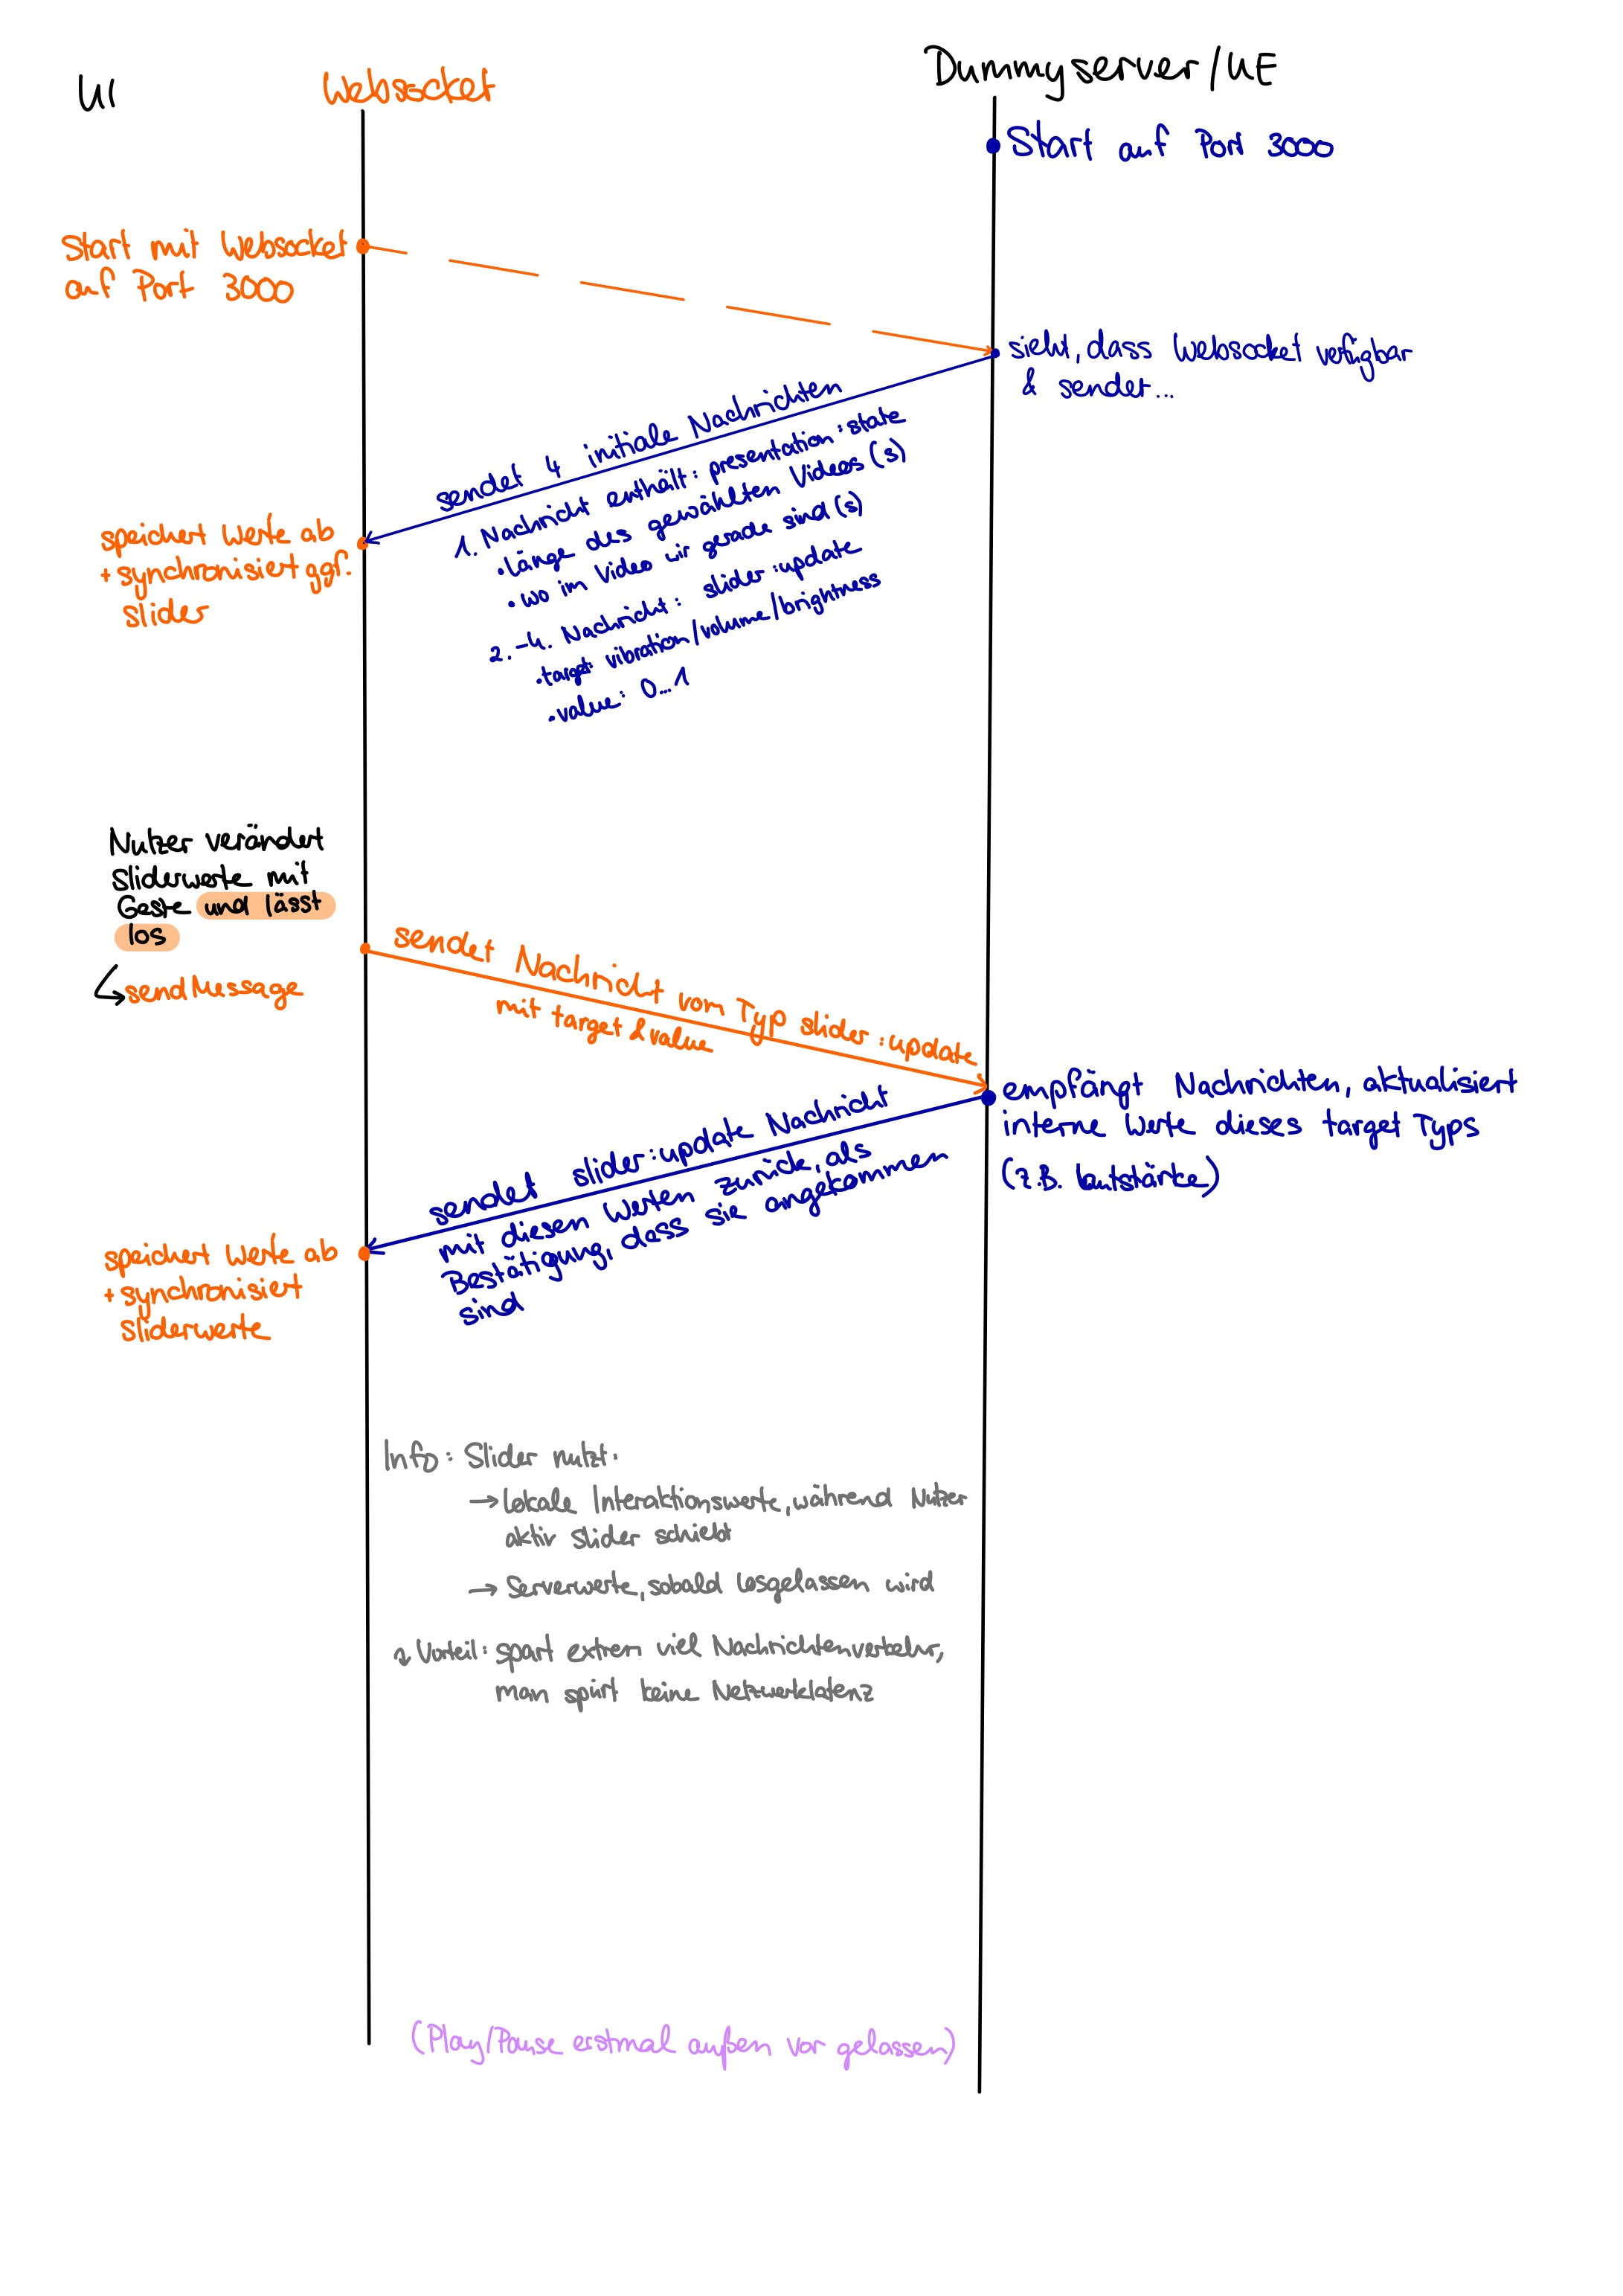
\includegraphics[width=0.9\linewidth]{content/diagrams/communication_flow.png}
\caption{Ablauf der WebSocket-basierten Eventkommunikation zwischen Overlay und Zielanwendung. Nach der Initialisierung werden Zustandsinformationen wie Menüstruktur oder Parameterwerte an das Overlay übertragen. Während der Interaktion sendet das Overlay abstrahierte Ereignisse an die Zielanwendung, welche diese verarbeitet und bei Bedarf synchronisierte Werte zur Bestätigung zurückgibt.}
\label{fig:communication_flow}
\end{figure}


\subsubsection{Anwendungsfall Präsentationssteuerung}
Für den Anwendungsfall der Präsentationssteuerung, und somit für alle Szenarien, die vorgerenderte Inhalte nutzen, ergeben sich besondere Anforderungen an die Interaktionslogik, da sowohl diskrete als auch kontinuierliche Eingaben unterstützt werden müssen.
Im Gegensatz zu reinen Menüinteraktionen kommen hierbei sowohl Button- als auch Slider-Elemente innerhalb eines Kontexts zum Einsatz.
Diese Interaktionsform wurde im Kontext der in Kapitel~\ref{sec:analyse} untersuchten atmosphärischen Szenarien mit vorgerendertem, narrativem Inhalt entwickelt, beispielsweise für die Steuerung eines Video-Mitschnitts im Fußballstadion. 
Ziel ist es, Nutzer:innen eine intuitive Kontrolle über die Wiedergabe zu ermög\-lichen, einschließlich Anhalten, Fortsetzen sowie Vor- und Zurückspulen des Materials.
Hierfür wurde ein spezieller Slider für den Zieltyp \texttt{presentation} implementiert, der, anders als die Defaultslider statt einer Prozentanzeige sowohl die Gesamtdauer des Videos als auch die aktuelle Wiedergabeposition abbildet. 
Während der Wiedergabe empfängt die Benutzungsoberfläche kontinuierlich Zeitstempel von der angebundenen Zielanwendung.
Diese werden genutzt, um den Fortschritt des Sliders dynamisch zu aktualisieren.

Ergänzend zum Slider enthält das entsprechende Menüelement eine Button-Interaktion zur Steuerung der Wiedergabe. 
Der Button schaltet zwischen den Zuständen \texttt{play} und \texttt{pause} um, und sendet entsprechend den aktuellen Status als Interaktionsereignis an die Zielanwendung.
Wird das Ende des Videos erreicht, sendet das System automatisch ein \texttt{pause}-Signal.
Bei einer erneuten Aktivierung durch die Nutzer:innen beginnt die Wiedergabe wieder am Anfang des Videos.


\subsection{Unterstützung mehrerer Projektionsflächen}
%(1) standardmäßig werden auf allen erkannten Screens electron fenster geöffnet und dann wird standard kamera auf alle gemappt
%(2) man kann im Konfigurationsmodus in electron die kamera pro bildschirm auswählen ODER im browser im Inkognito Tab pro fenster das auswählen
%(3) man kann mit modifikation von npm start command direkt bestimmte Bildschirme und bestimmte kamera mappings festlegen
%(4) es wird sichergestellt, dass bei der interaktion die aktivierungsgeste nur von der frontalen seite erkannt wird, indem abstand von kleinem finger und daumen gemessen wird (dafür wird schon vorher genutzter open Palm threshold mit offset verwendet, damit nicht noch ein parameter kalibriert werden muss - ist das überhaupt interessant?)
%(5) in browserversion werden kalibrierungskeys wahrscheinlich nicht auf alle übertragen - aber bei electron werden alle keys immer für alle bildschirme angewadnt - das ist tradeoff aber ist ja sowieso nur "gemütlichere Testvariante", also ist browser version nicht so wichtig
%(6) um electron fenster drei mal zu öffnen, aber einen webscoket zu nutzen, wird IPC angewandt. dadurch werden drei fenster als renderer von electron aufgerufen, die dann mit einer main kommunizieren und dann spricht der mein process den websocket an und macht die kommunikation mit dem Server -- alles mal vernünftig aufschreiben}

Das entwickelte Interaktionssystem wurde für den Einsatz im Multisensorischen Interaktionsraum konzipiert, in dem die Inhalte auf drei Projektionsflächen rund um die Nutzer:innen dargestellt werden.
Daraus ergibt sich die Anforderung, das Overlay nicht nur auf einem einzelnen Bildschirm, sondern parallel auf mehreren Ausgabeflächen bereitzustellen.
Das System wurde deshalb so erweitert, dass für jede relevante Projektionsfläche ein eigenes Overlay-Fenster erzeugt werden kann.
Auf diese Weise lässt sich das Marking-Menu jeweils direkt auf derjenigen Leinwand öffnen, auf der die Interaktion stattfinden soll.
In der Electron-basierten Umsetzung werden hierfür mehrere Fenster instanziiert, die jeweils als eigenständige Renderer-Prozesse ausgeführt werden.
Jedes dieser Fenster stellt ein eigenes Overlay auf einer Projektionsfläche dar, übernimmt die lokale Darstellung des Menüs und verarbeitet die zugehörigen Interaktions\-zustände.
Die übergeordnete Koordination erfolgt jedoch zentral über den Main-Prozess von Electron.
Dieser verwaltet die Kommunikation zwischen den Fenstern und bündelt zugleich die WebSocket-Kommunikation mit der angebundenen Zielanwendung.
Dadurch ist es möglich, mehrere Overlay-Fenster parallel zu betreiben, ohne für jede Projektionsfläche eine separate Netzwerkverbindung aufbauen zu müssen.
Die Kommunikation zwischen Renderer- und Main-Prozess erfolgt über \textit{Electron Inter-Process Communication (IPC)} \parencite{electronIPCdocumentation}, sodass Zustandsinformationen und Interaktionsereignisse innerhalb der Anwendung effizient verteilt werden können. Der Prozess ist in Abbildung \ref{fig:ipc_diagram} veranschaulicht.

\begin{figure}[htbp]
    \centering
    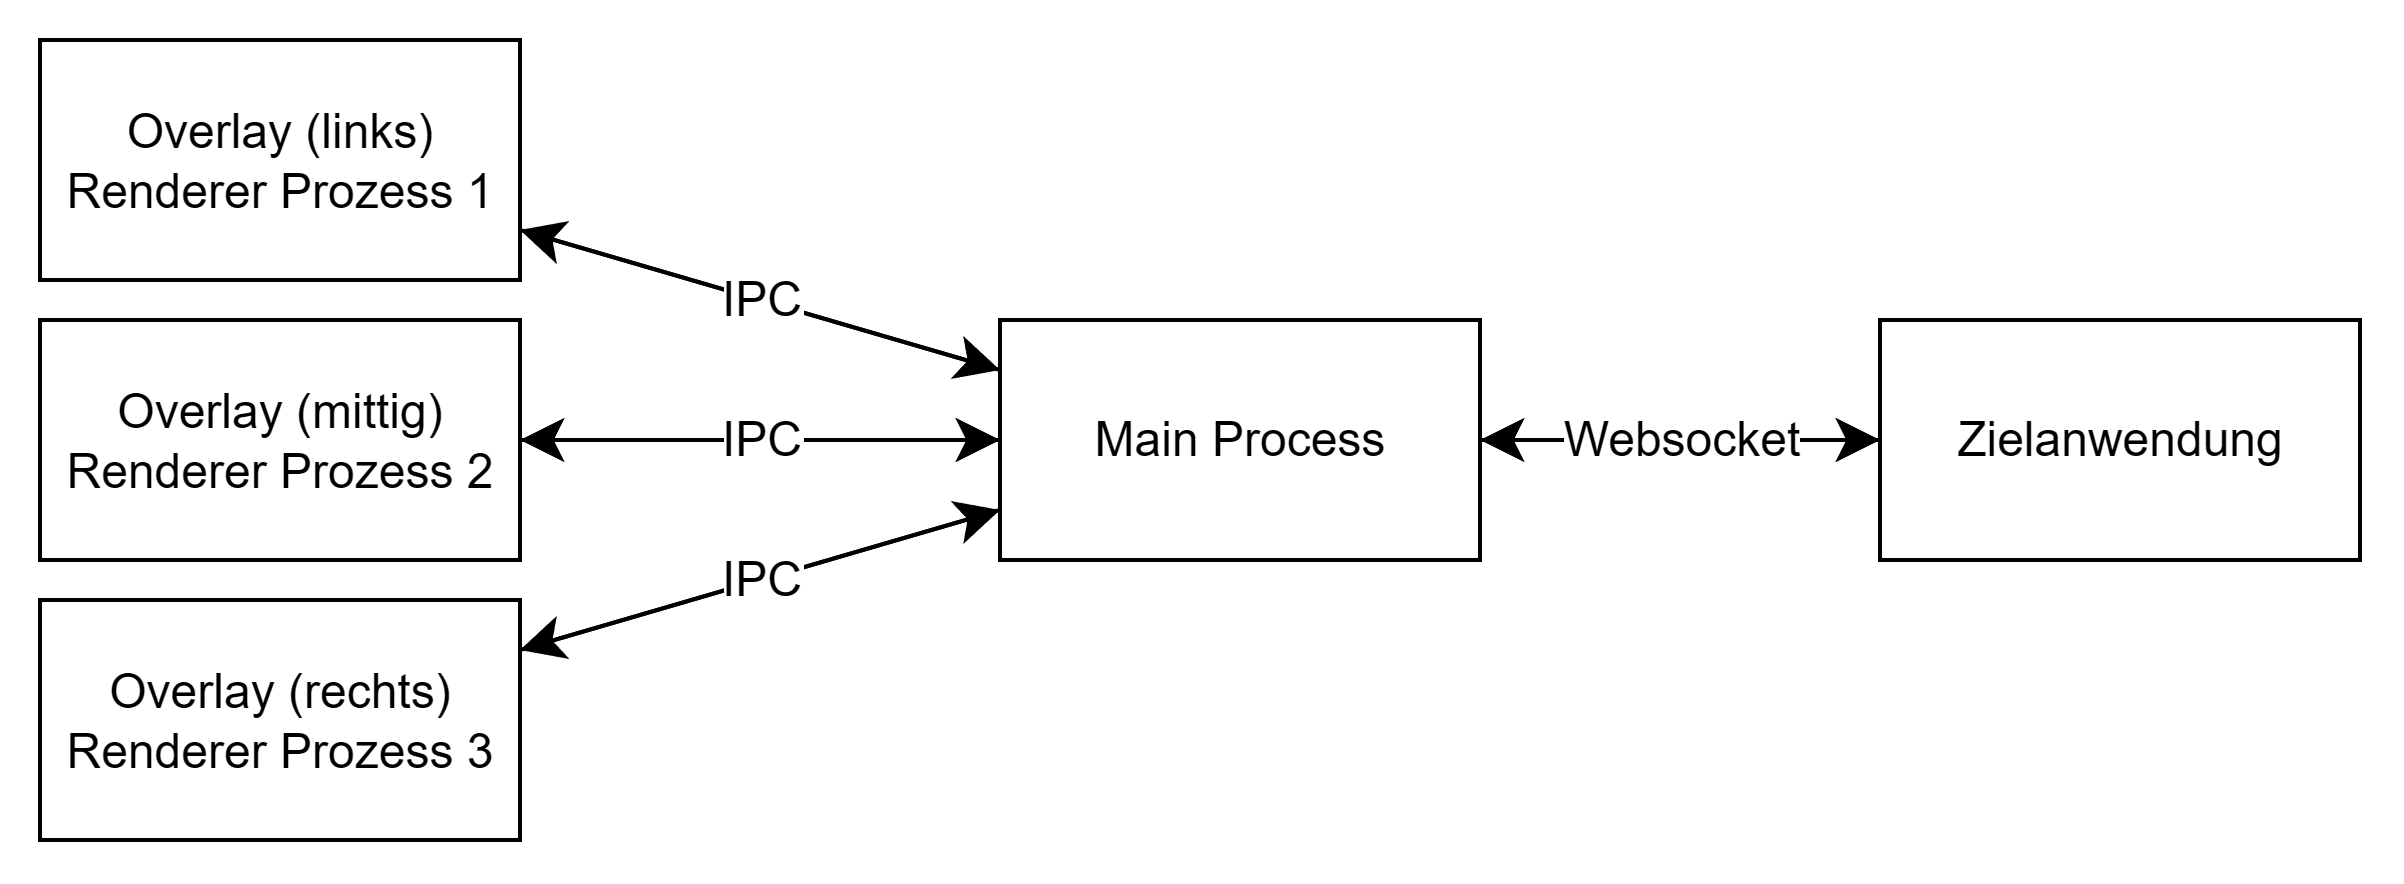
\includegraphics[width=0.9\linewidth]{content/diagrams/ipc_diagram}
    \caption{Architektur des Mehrbildschirmbetriebs. Für jede Projektionsfläche wird ein eigenes Overlay-Fenster als Renderer-Prozess erzeugt. Diese sind über Electron-IPC mit dem Main Process verbunden, der die zentrale WebSocket-Kommunikation mit der Zielanwendung übernimmt.}
    \label{fig:ipc_diagram}
\end{figure}

Eine besondere Herausforderung im Mehrbildschirmbetrieb besteht in der Zuordnung von Kameraquellen zu den jeweiligen Projektionsflächen.
Im einfachsten Fall kann dieselbe Standardkamera zunächst auf mehrere Fenster angewendet werden, um das System schnell zu starten und grundlegende Funktionen zu testen.
Für den tatsächlichen Einsatz im Interaktionsraum ist jedoch eine gezielte Zuordnung erforderlich, da für jede Leinwand eine Kamera zur Verfügung steht. Dafür wurden mehrere Konfigurationsmöglichkeiten vorgesehen. Zum einen kann im Konfigurationsmodus innerhalb des Overlays eine Kamera auf jedem Bildschirm ausgewählt werden (siehe Abbildung \ref{fig:select_kamera_interface}).
Zum anderen lässt sich in der browserbasierten Variante die gewünschte Kamera direkt im jeweiligen Fenster festlegen. Zusätzlich besteht die Möglichkeit, beim Start der Anwendung feste Zuordnungen von Bildschirmen und Kameras über Startparameter vorzugeben. Diese unterschiedlichen Konfigurationswege erleichtern sowohl das flexible Testen als auch den reproduzierbaren Einsatz in der Zielumgebung.

\begin{figure}[htbp]
    \centering
    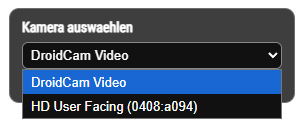
\includegraphics[width=0.6\linewidth]{content/images/select_kamera_interface}
    \caption{Benutzungsoberfläche, die im Konfigurationsmodus auf jedem aktiven Bildschirm angezeigt wird, um die zugehörige Kamera auszuwählen.}
    \label{fig:select_kamera_interface}
\end{figure}

Damit eine Interaktion nur auf der jeweils passenden Leinwand ausgelöst wird, muss das System sicherstellen, dass Aktivierungsgesten nicht gleichzeitig oder versehentlich auf mehreren Projektionsflächen interpretiert werden.
Dies ist insbesondere dann relevant, wenn eine Hand von mehreren Kameras teilweise erfasst wird. Zur Reduktion solcher Fehlaktivierungen wurde die Aktivierungsgeste so definiert, dass sie nur bei einer ausreichend frontalen Handausrichtung erkannt wird. Hierzu wird neben den allgemeinen Merkmalen der offenen Hand zusätzlich die relative Anordnung ausgewählter Landmarken berücksichtigt. Insbesondere der Abstand zwischen Daumen und kleinem Finger wird genutzt, um abzuschätzen, ob die Handfläche zur Kamera orientiert ist (siehe Abbildung \ref{fig:hand_frontal_site}). Dadurch wird erreicht, dass das Menü bevorzugt auf derjenigen Leinwand aktiviert wird, vor der die Nutzer:innen tatsächlich stehen, während seitlich erfasste Hände die Aktivierung nicht oder nur deutlich seltener auslösen.

\begin{figure}[htbp]
    \centering
    \begin{subfigure}[t]{0.32\textwidth}
        \centering
        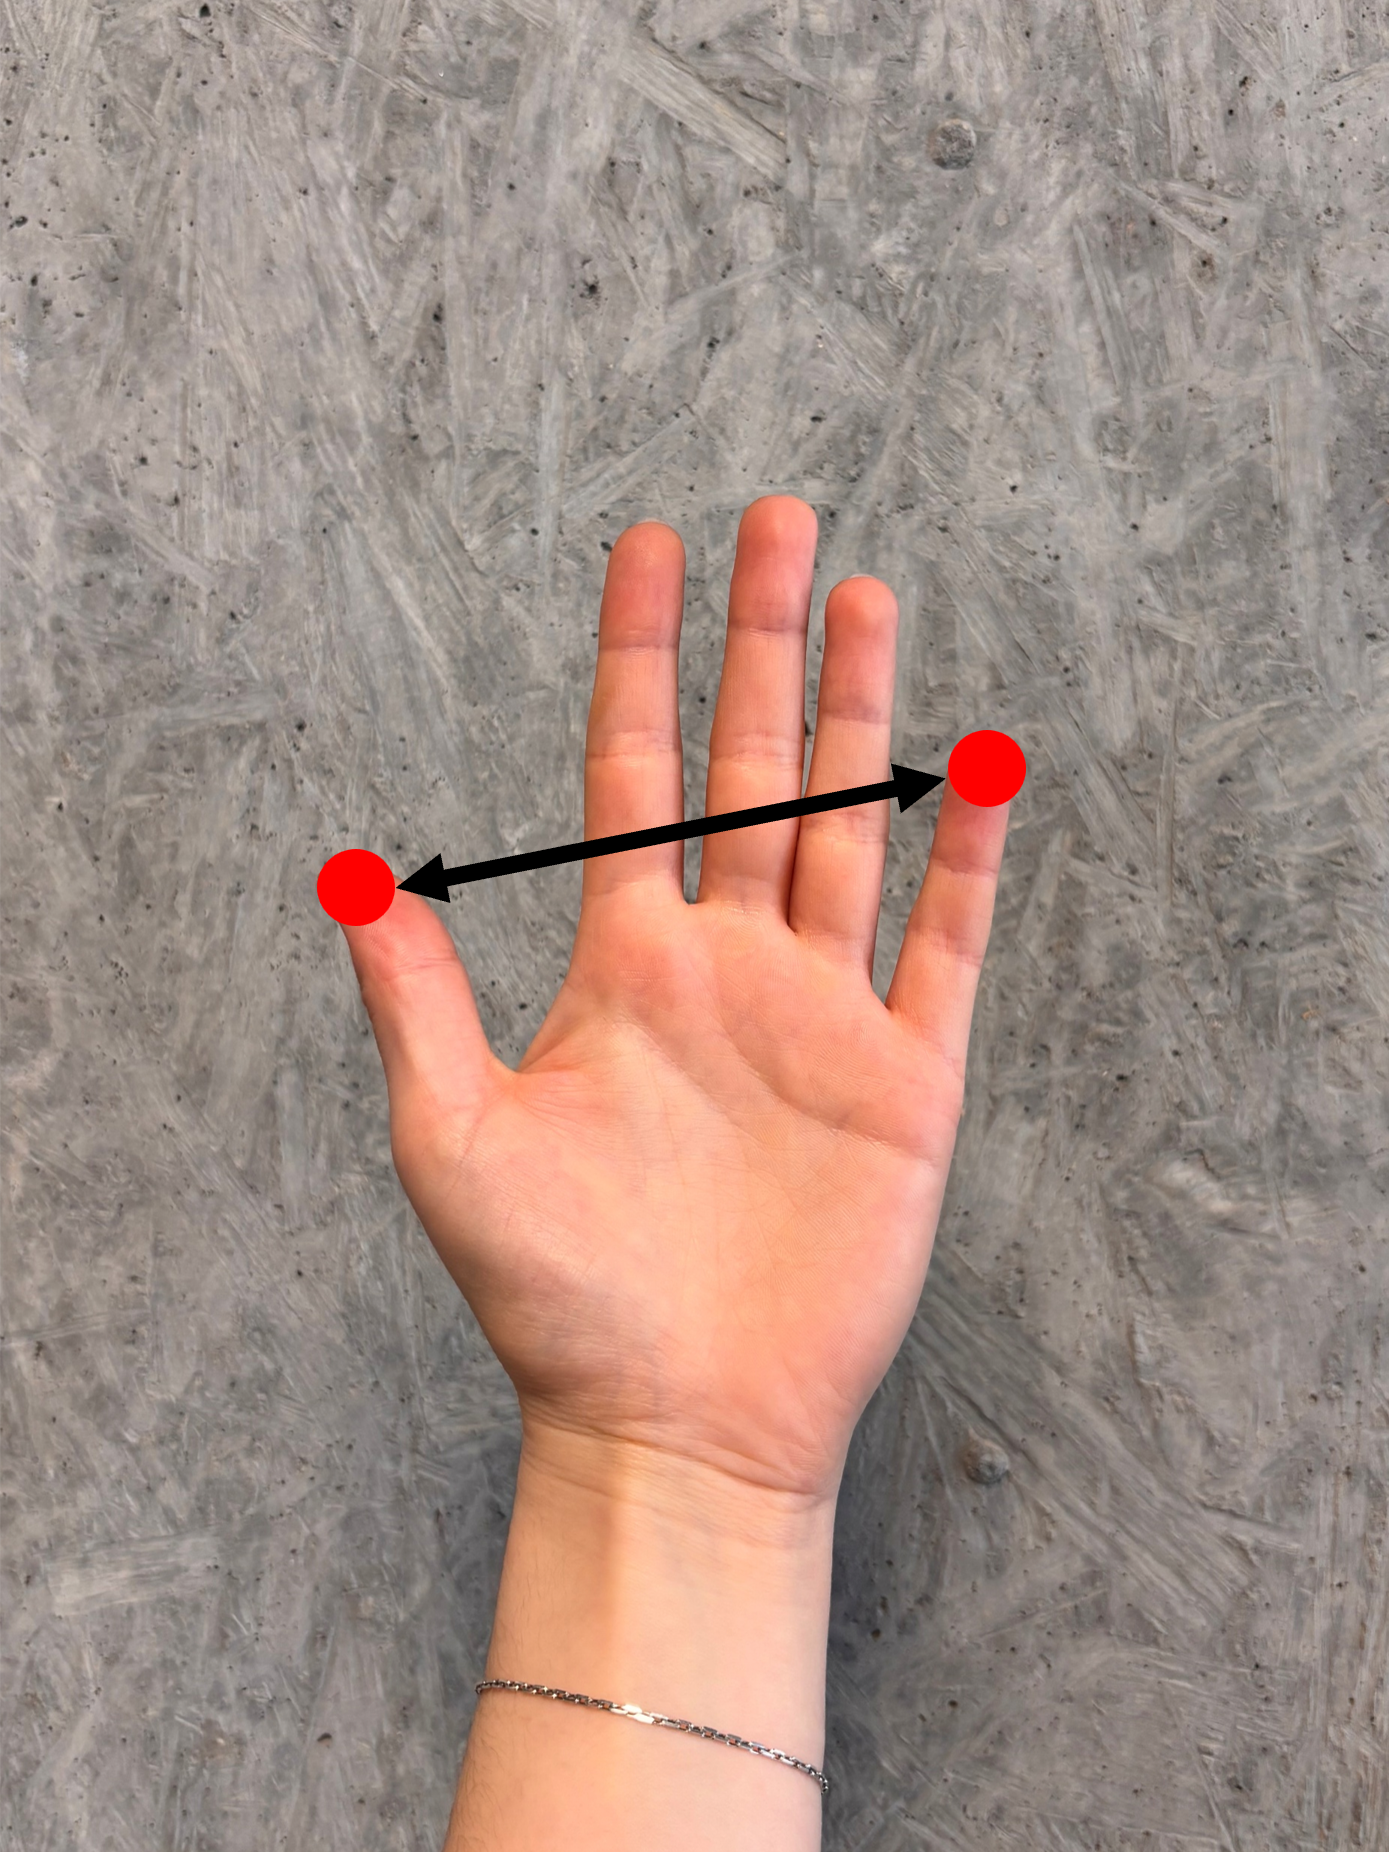
\includegraphics[width=\linewidth]{content/images/hand_frontal.png}
        \caption{Aktivierungsgeste wird erkannt.}
        \label{fig:hand_frontal}
    \end{subfigure}
    \hfill
    \begin{subfigure}[t]{0.32\textwidth}
        \centering
        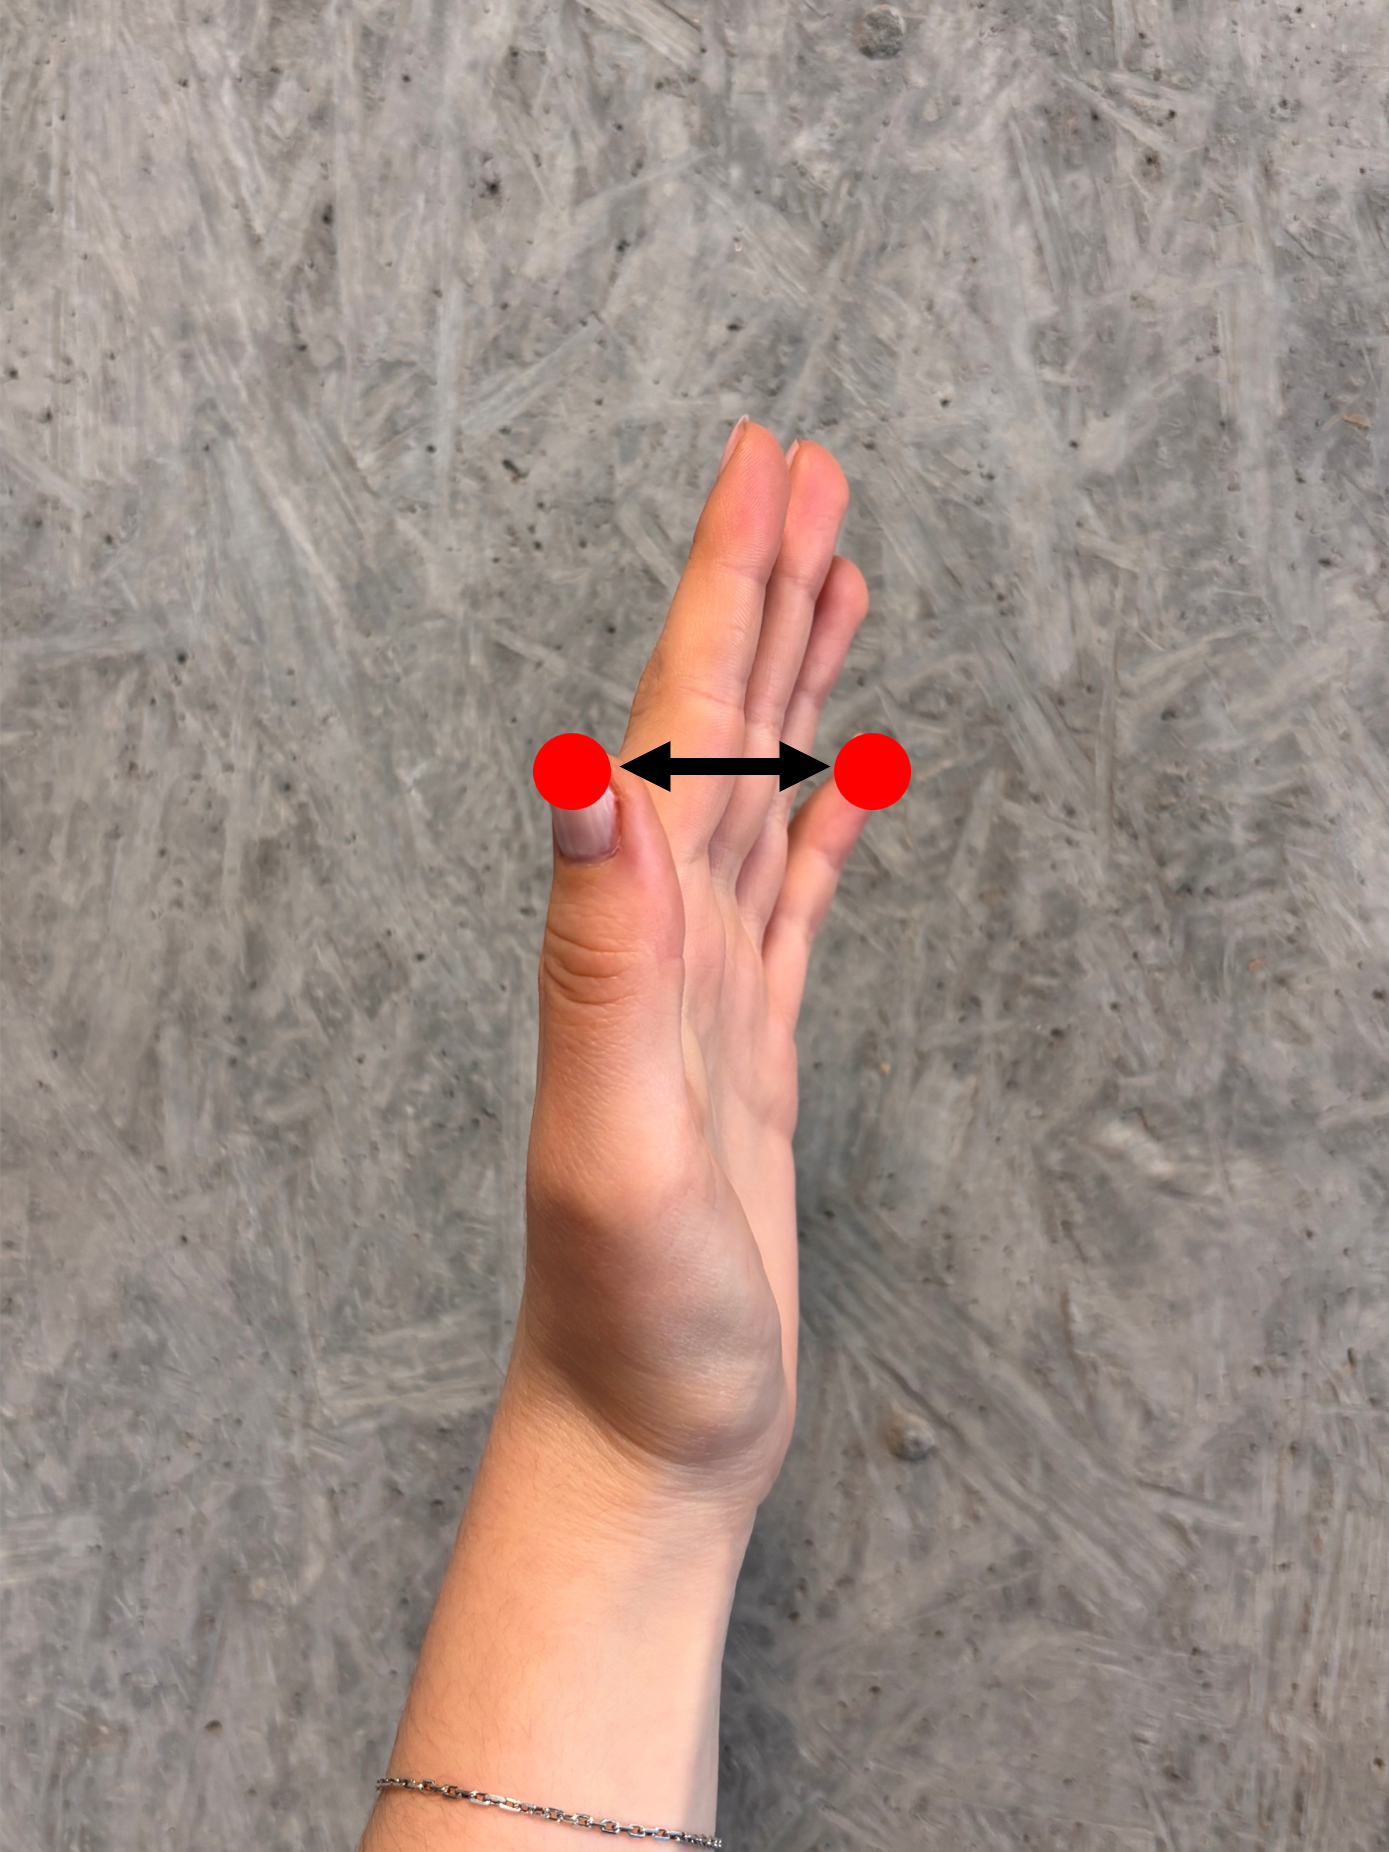
\includegraphics[width=\linewidth]{content/images/hand_half_frontal.png}
        \caption{Aktivierungsgeste wird aus dieser Perspektive nicht erkannt.}
        \label{fig:hand_half_frontal}
    \end{subfigure}
    \hfill
    \begin{subfigure}[t]{0.32\textwidth}
        \centering
        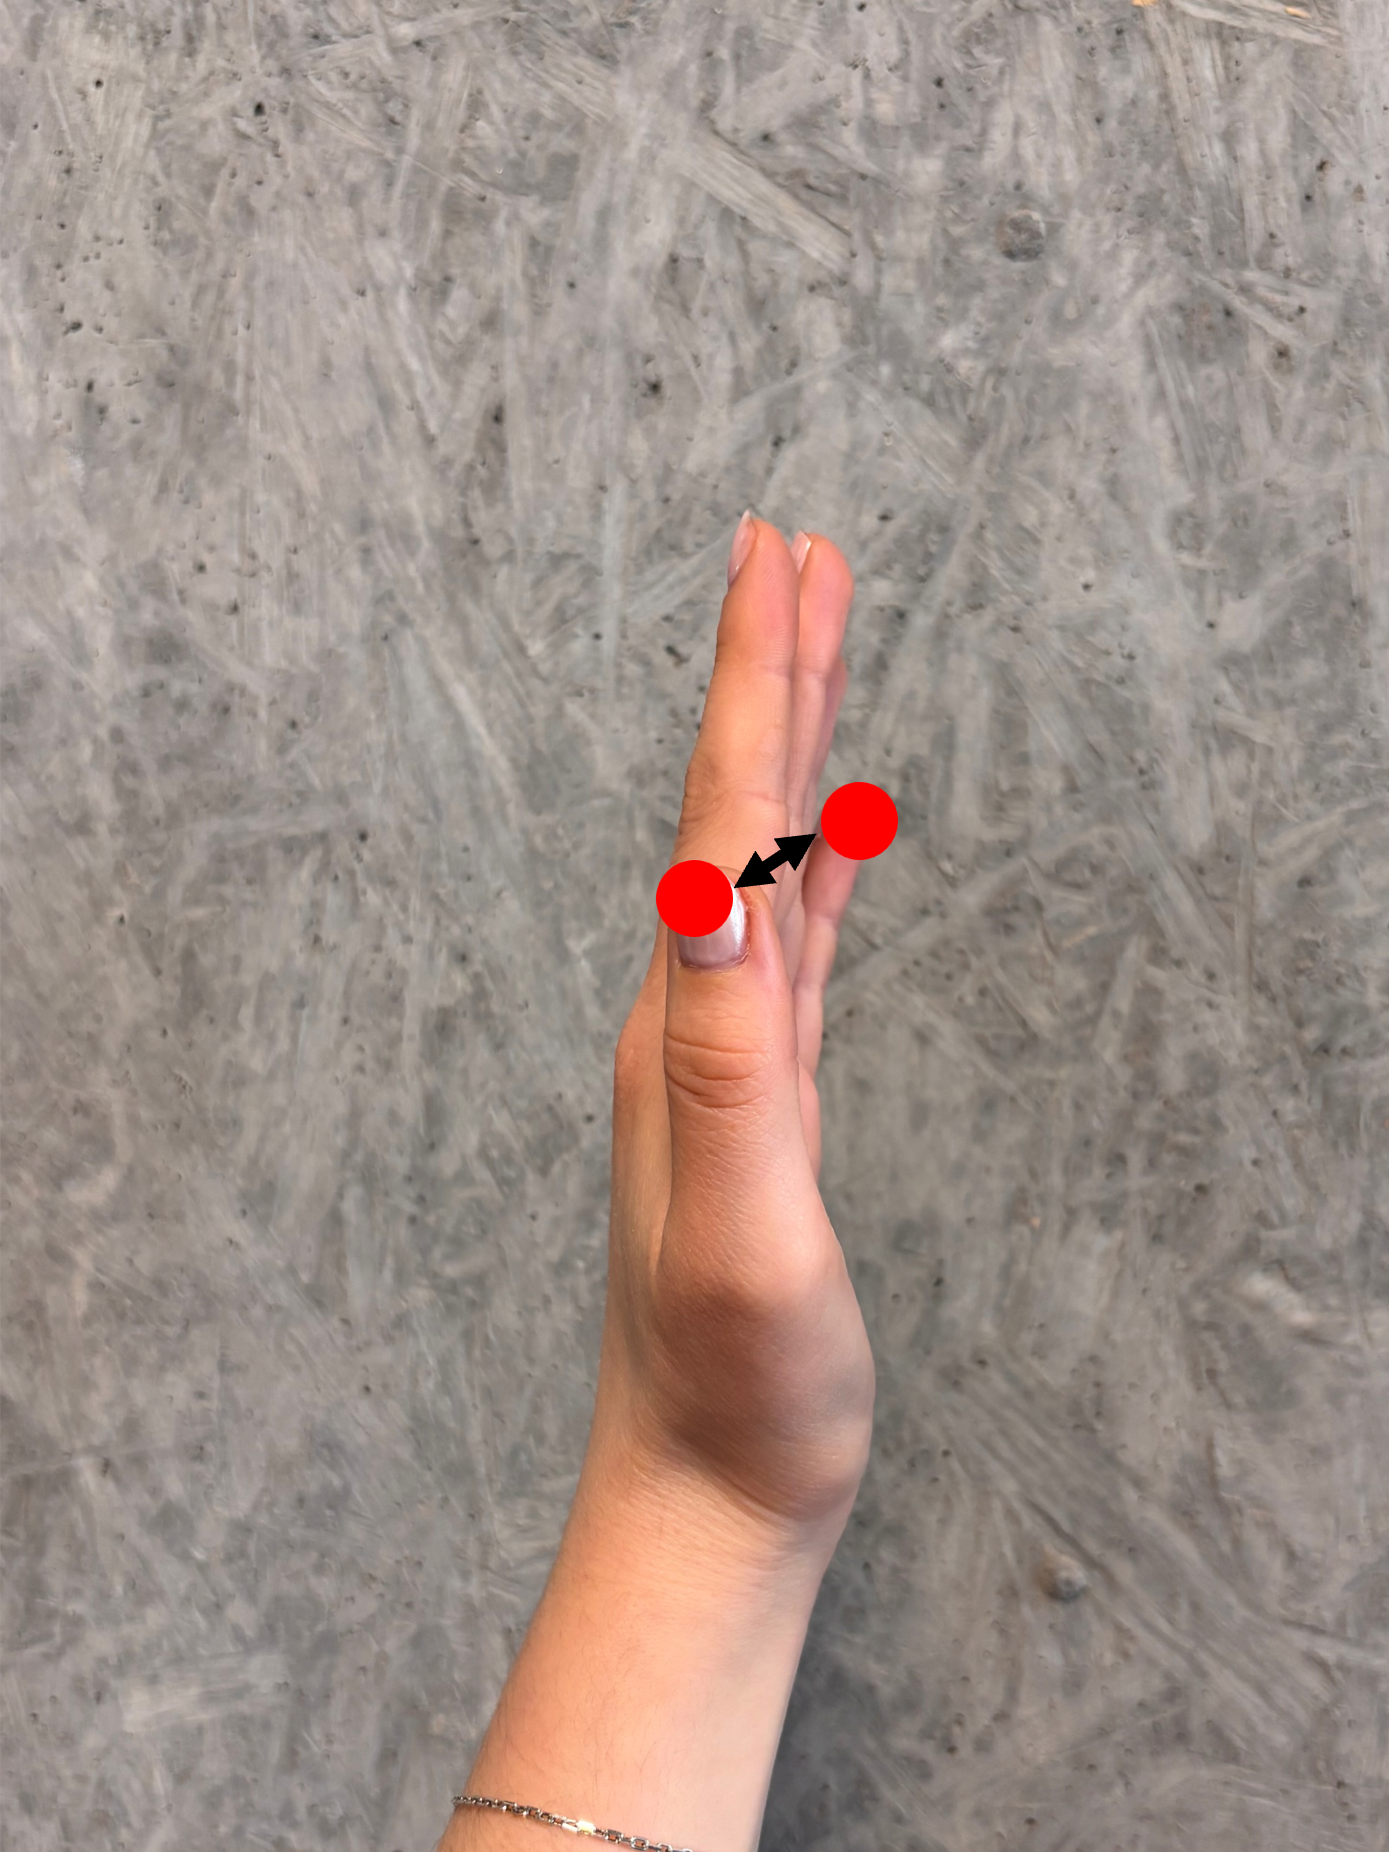
\includegraphics[width=\linewidth]{content/images/hand_site.png}
        \caption{Aktivierungsgeste wird aus dieser Perspektive nicht erkannt.}
        \label{fig:hand_site}
    \end{subfigure}
    \caption{Handorientierung: gültige und ungültige Aktivierungsgeste}
    \label{fig:hand_frontal_site}
\end{figure}

Die Mehrbildschirmarchitektur erweitert das Interaktionssystem somit um eine räumliche Dimension.
Das Overlay ist nicht mehr auf einen einzelnen Anzeigekontext beschränkt, sondern kann als verteilte Interaktionsschicht innerhalb des gesamten Multisensorischen Interaktionsraums eingesetzt werden. Gleichzeitig bleibt die grundlegende Systemarchitektur erhalten: Handtracking, Interaktionslogik, Darstellung und Zielanwendung bleiben voneinander getrennt. Dadurch kann das System auch im Mehrbildschirmbetrieb modular konfiguriert, getestet und an unterschiedliche räumliche Setups angepasst werden.


\subsection{Entwicklungs- und Testumgebung}
\label{sec:development}
Zur Unterstützung der Implementierung wurden mehrere Werkzeuge eingesetzt, die insbesondere die Entwicklung, das Testen und das Debugging des Interaktionssystems erleichtern sollen.
Eine zentrale Rolle spielte dabei ein Mock-Server, der das Verhalten einer Zielanwendung simuliert. Dieser Server stellt initiale Menü- und Statusdaten bereit, verarbeitet eingehende Interaktionsnachrichten des Overlays und sendet entsprechende Zustandswerte zurück. Dadurch konnte die Kommunikationsschnittstelle unabhängig von einer laufenden Zielanwendung entwickelt und getestet werden.

Zusätzlich wurde ein Offline-Modus vorgesehen, in dem das System mit lokalen Testdaten arbeitet. Dadurch kann die Benutzungsoberfläche auch ohne aktive WebSocket-Verbindung betrieben werden, was isolierte Tests einzelner Komponenten ermöglicht. Dafür wurde das System zusätzlich als browserbasierte Variante bereitgestellt, wodurch eine einfache Demonstration und ein schneller Zugriff auf das Interaktionssystem ohne lokale Installation möglich wurde.

Ergänzend zu Mock-Server und Offline-Modus wurde das Interaktionssystem bereits exemplarisch an eine konkrete Testanwendung durch einen Entwickler des MIR angebunden. Dabei wurden vorgerenderte Videoinhalte über die entwickelte WebSocket-Schnittstelle gesteuert. Als Testfall diente unter anderem ein kurzes Video einer Berglandschaft, das sich aufgrund seiner geringen Länge besonders für wiederholte Tests der Wiedergabe- und Timeline-Steuerung eignete. Über das Marking-Menu konnten dabei sowohl die Lautstärke als auch der Wiedergabezustand sowie das Vor- und Zurückspulen des Videos gesteuert werden. Da dieses Testszenario nicht Bestandteil der in Abschnitt~\ref{sec:analyse} untersuchten Szenarien war, diente es primär der technischen Überprüfung der Anbindung.
Abbildung~\ref{fig:berg_testanwendung} zeigt beispielhaft die angebundene Testanwendung im MIR.

\begin{figure}[H]
    \centering
    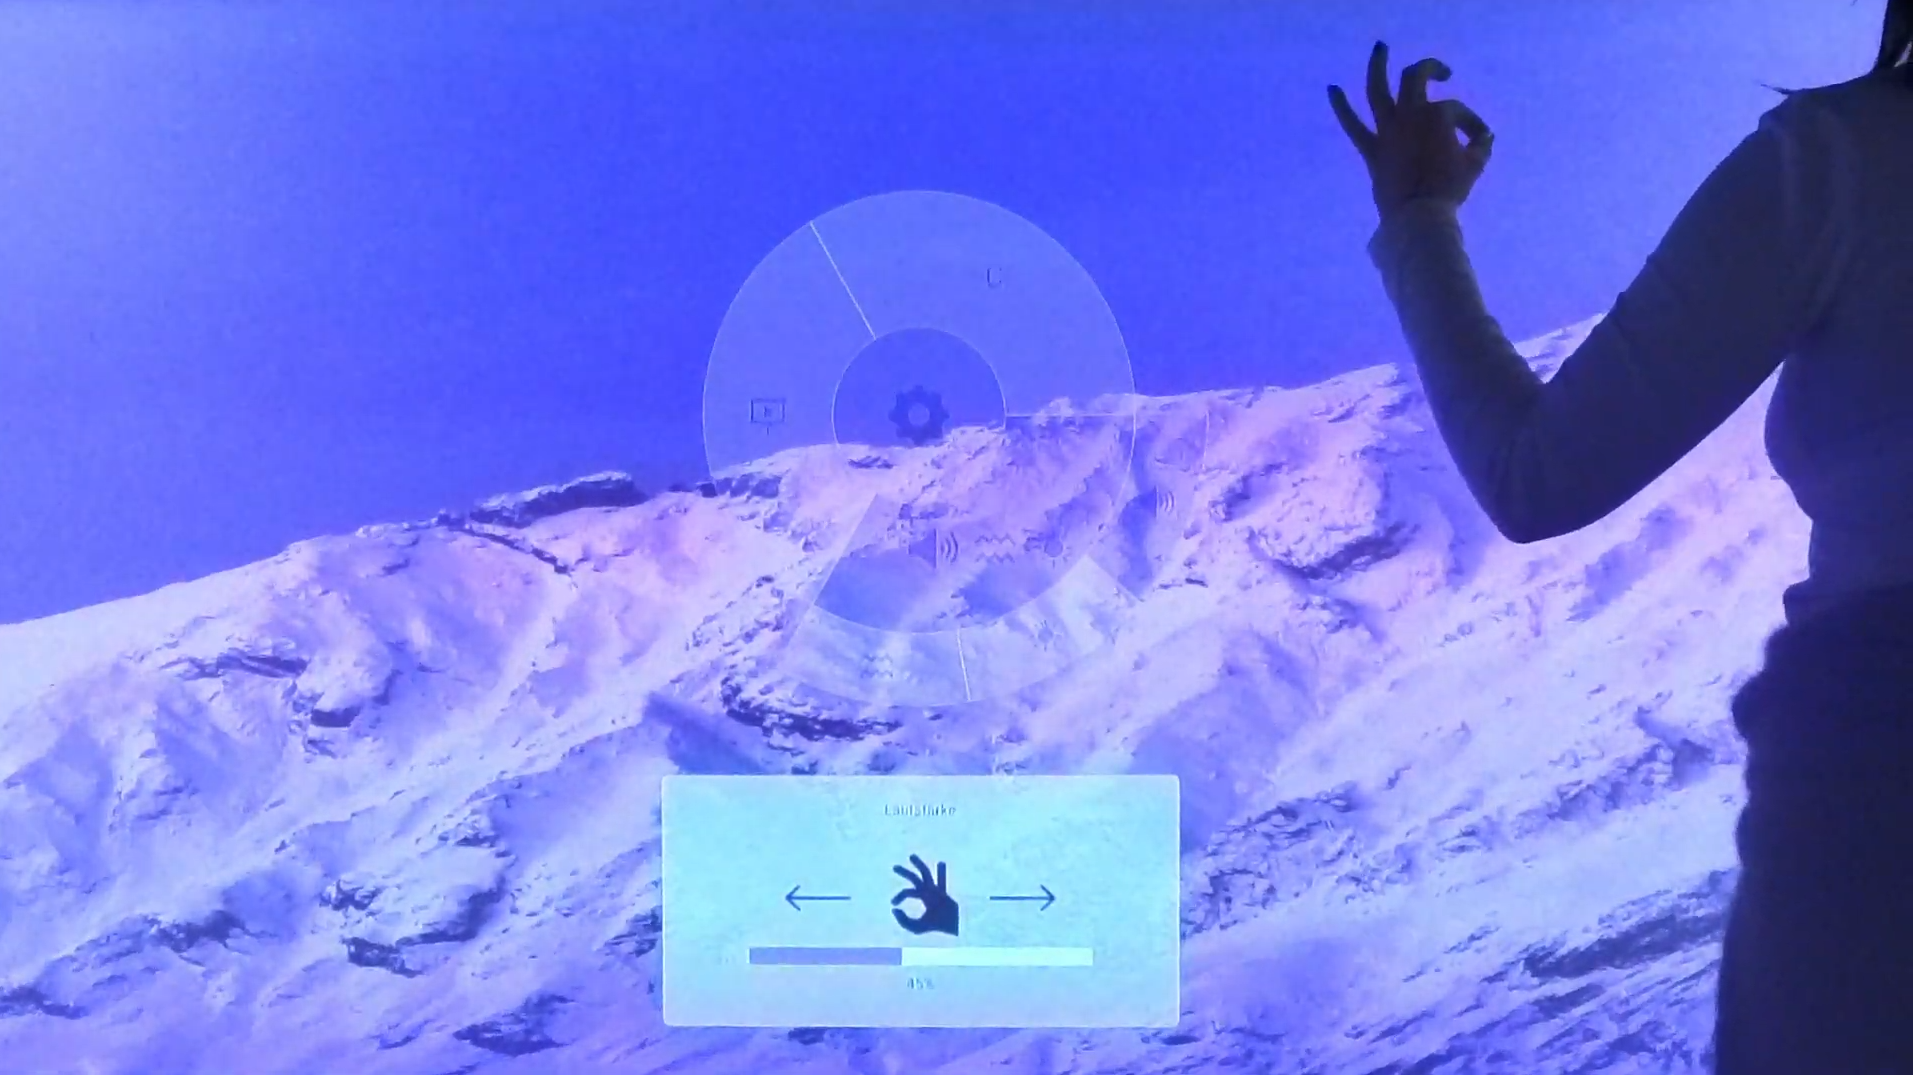
\includegraphics[width=0.8\linewidth]{content/images/vieo-still.png}
    \caption{Ausschnitt aus einem Interaktionsvideo des Berglandschaftsszenarios mit vorgerendertem Videoinhalt. Die Umgebung wird durch eine Nutzerin über das Marking-Menu gesteuert.}
    \label{fig:berg_testanwendung}
\end{figure}

Neben diesen angebundenen Tests erfolgte ein Großteil der Entwicklung auf einem Laptop-System, während Tests des vollständigen Interaktionssystems im Multisensorischen Interaktionsraum durchgeführt wurden. Da die Größe und Position des Marking-Menus auf den großflächigen Projektionen deutlich anders wahrgenommen werden als auf einem Laptopdisplay, wurden zusätz\-liche Kalibrierungsfunktionen implementiert.
Über Tastaturkürzel konnten während der Ent\-wick\-lungs\-phase Parameter wie die Position, Skalierung und Darstellung des Menüs angepasst werden. Ebenso konnten Schwellwerte der Gestenerkennung sowie Dwell-Zeiten zur Interaktionsauslösung dynamisch verändert werden. Diese Funktionen erleichterten die Feinabstimmung des Interaktionssystems in unterschiedlichen Testumgebungen.

Diese Werkzeuge unterstützten insbesondere die iterative Entwicklung und ermöglichten eine schrittweise Überprüfung der einzelnen Systemkomponenten. Die Tests wurden dabei nicht ausschließlich isoliert durchgeführt, sondern erfolgten auch im Multisensorischen Interaktionsraum in Zusammenarbeit mit einem Entwickler des Systems sowie dem Betreuer der Arbeit. Dadurch konnten praktische Aspekte der Integration und Nutzung frühzeitig berücksichtigt werden.


\subsection{Integration der Systemkomponenten}
Die beschriebenen Komponenten bilden gemeinsam das entwickelte Interaktionssystem für den Multisensorischen Interaktionsraum. 
Das Handtracking liefert kontinuierlich Handlandmarkeninformationen der Nutzer:innen, aus denen Cursorbewegungen und Interaktions\-zustände abgeleitet werden.
Diese Informationen steuern das im Electron-Overlay dargestellte Marking-Menu sowie dessen Interaktionslogik.
Über die WebSocket-Schnittstelle werden Interaktionsereignisse an die angebundene Zielanwendung übertragen und mit deren Zustand synchronisiert. 
Die datengetriebene Menüstruktur ermöglicht es dabei, die Interaktionsoberfläche flexibel an unterschiedliche Anwendungsszenarien anzupassen.
Durch die modulare Architektur bleiben Tracking, Benutzungsoberfläche und Zielanwendung voneinander getrennt, wodurch das System flexibel an unterschiedliche Anwendungsszenarien angepasst werden kann.

Das entwickelte System stellt damit eine prototypische Umsetzung körper\-basierter Interaktion im MIR dar, die als Grundlage für zukünftige Erweiterungen und Anwendungsszenarien dienen kann.


\clearpage
\appendix
\section*{Anhang}

\begin{landscape}
\begin{figure}[p]
    \centering
    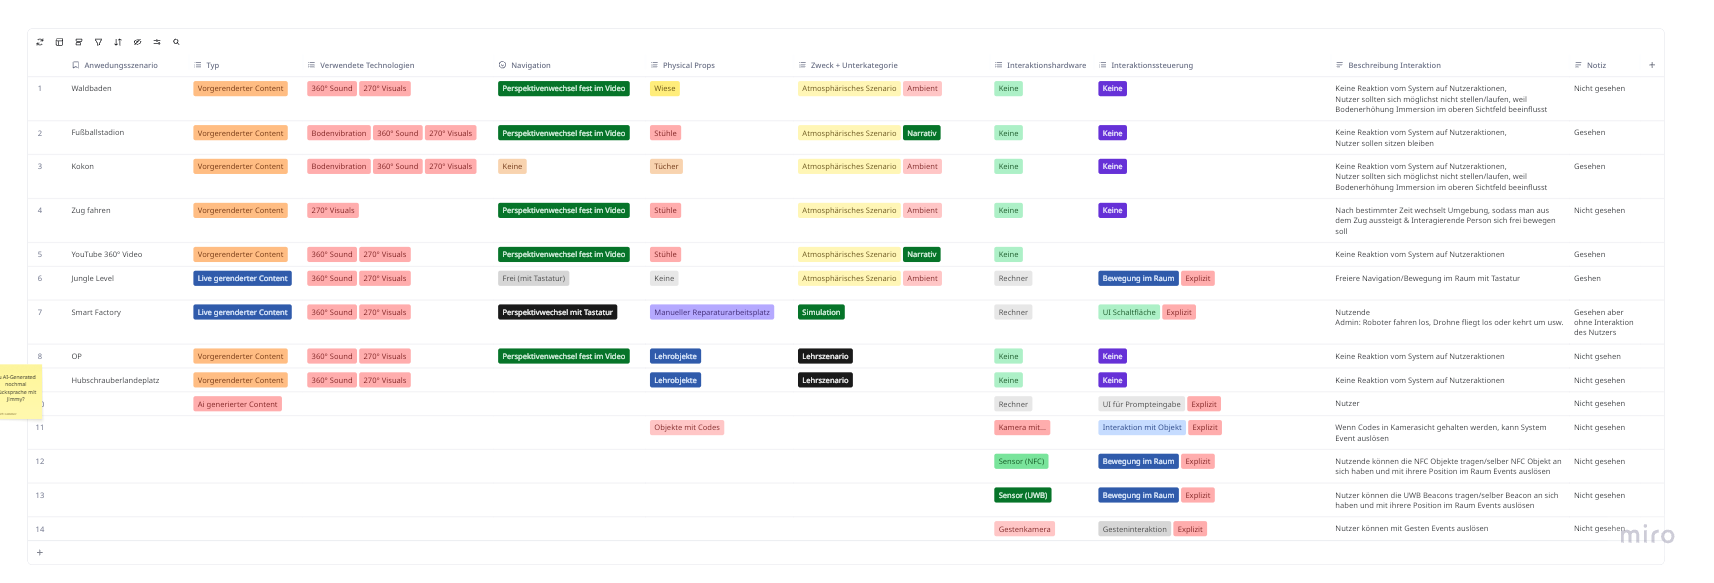
\includegraphics[width=\linewidth]{content/images/anwendungsfallanalyse.png}
    \caption{Übersicht über analysierte Anwendungsszenarien}
    \label{fig:anwendungsszenarien}
\end{figure}
\end{landscape}

\begin{landscape}
\begin{figure}[p]
    \centering
    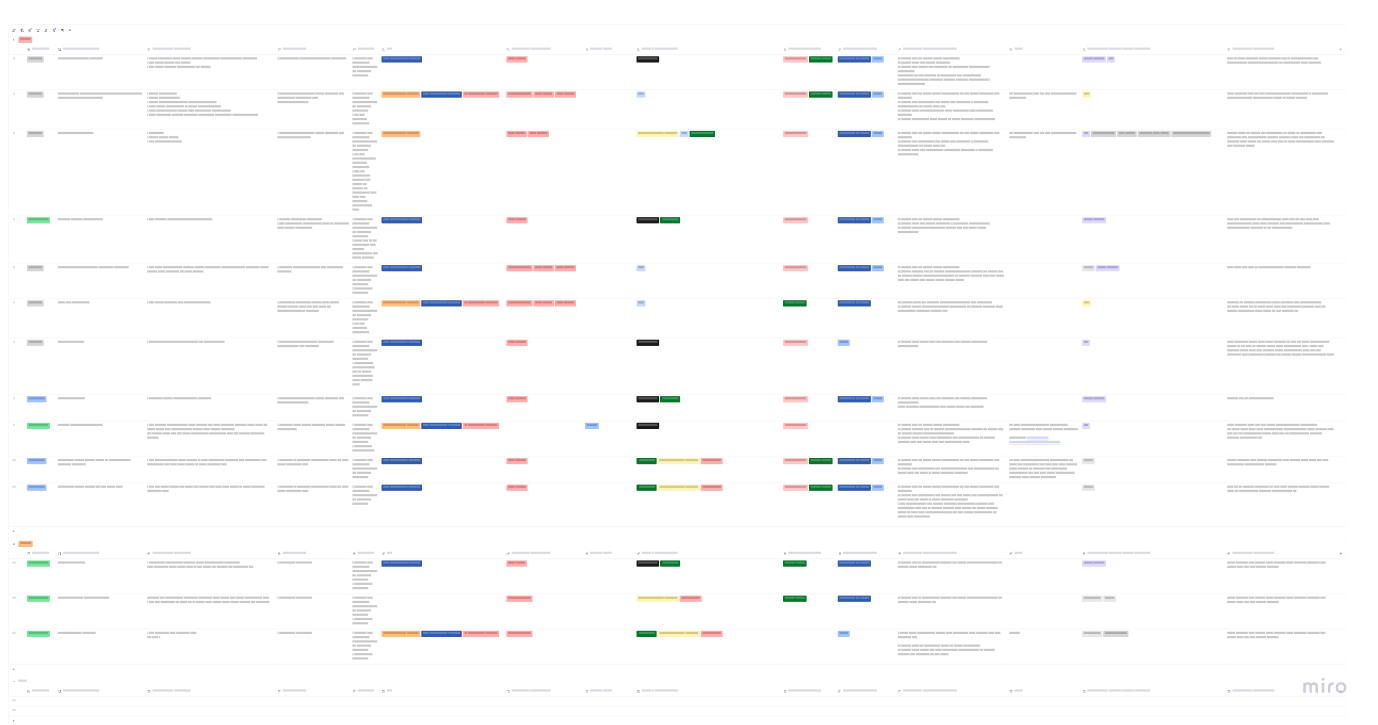
\includegraphics[width=\linewidth]{content/images/interaktionsmoeglichkeiten.png}
    \caption{Übersicht potenzieller körperbasierter Interaktionsformen}
    \label{fig:interaktionsmoeglichkeiten}
\end{figure}
\end{landscape}

\begin{longtable}{p{0.25\linewidth} p{0.7\linewidth}}
    \caption{Übersicht untersuchter Interaktionsansätze im MIR} \label{tab:interaktionsansatz} \\

    \toprule
    \textbf{Kategorie} & \textbf{Beschreibung} \\
    \midrule
    \endfirsthead

    \toprule
    \textbf{Kategorie} & \textbf{Beschreibung} \\
    \midrule
    \endhead

    \midrule
    \multicolumn{2}{r}{\textit{Fortsetzung auf nächster Seite}} \\
    \endfoot

    \bottomrule
    \endlastfoot

% --- EINTRAG ---
    \textbf{Name} & Zusatzinformationen anzeigen \\

    \textbf{Beschreibung} & Durch Auslösen eines Events (beispielsweise Zeigen auf Objekt oder näheres Herantreten) werden zusätzliche Informationen zu Objekten oder Umgebungen angezeigt. \\

    \textbf{Interaktionsmodus} & Explizit \\

    \textbf{Interaktionstechnik} & Selektion \\

    \textbf{Inhaltstyp} & hauptsächlich Live gerenderter Inhalt \\

    \textbf{Technologien} & 270° Visuals \\

    \textbf{Zweck/Unterkategorie} & Lehrszenario \\

    \textbf{Interaktionshardware} & Kamera zur Gestenerkennung, Sensor (UWB) \\

    \textbf{Interaktionssteuerung} & Bewegung im Raum \\

    \textbf{Eignung MIR} & Nutzbar für Smart Factory, OP; Je nach Szenario sinnvoll, beispielsweise in Lehrszenarien, um selbstständig Zusatzinformationen zu erhalten  \\

    \midrule

% --- NÄCHSTER EINTRAG ---
    \textbf{Name} & Administrative Steuerung der Lautstärke, Helligkeit, Virbationsintensität \\

    \textbf{Beschreibung} & Einstellungsmöglichkeit von globaler Lautstärke, Helligkeit und Vibrationsintensität (denkbar mit Integration von lokaler Aktivierung/Deaktivierung von Licht- oder Soundquellen)  \\

    \textbf{Interaktionsmodus} & Explizit \\

    \textbf{Interaktionstechnik} & Selektion \\

    \textbf{Inhaltstyp} & Alle \\

    \textbf{Technologien} & 270° Visuals, 360° Sound, Bodenvibration \\

    \textbf{Zweck/Unterkategorie} & Alle \\

    \textbf{Interaktionshardware} & Kamera zur Gestenerkennung \\

    \textbf{Interaktionssteuerung} & Geste, Bewegung im Raum \\

    \textbf{Eignung MIR} & Sehr geeignet, da es für alle Szenarien anwendbar ist. Administratoren sind losgelöst von Tastatur und Maus und können im MIR Einfluss der Änderungen wahrnehmen. \\

    \midrule



\end{longtable}]

\appendix
\section{Glossar}

\clearpage
\section{Literaturverzeichnis}
\printbibliography[heading=none]

% TODO: hier nochmal gucken, wie Seite nummeriert sein muss
\clearpage
\section{Abbildungsverzeichnis}
\listoffigures

\pagenumbering{roman} % bis hier römische Nummerierung

\end{document}

